% UCI Ph.D. Dissertation - Arnold K. Seong
% Bayesian Variable Selection in Semi-Parametric Settings

\documentclass[12pt, fleqn]{ucithesis}

% Standard packages
\usepackage{amsmath}
\usepackage{amsthm}
\usepackage{amssymb}
\usepackage{array}
\usepackage{graphicx}
\usepackage{natbib}
\usepackage{relsize}
\usepackage[titletoc]{appendix}
\usepackage{bm}
\usepackage{bbm}

% Layout / formatting packages
\usepackage{caption}
\usepackage{subcaption}
\usepackage{multirow}
\usepackage{tabularx}
\usepackage{booktabs}
\usepackage{parskip}
\usepackage{xcolor}
\usepackage{epigraph}
\setlength\epigraphwidth{.55\textwidth}
% \usepackage[margin=1in]{geometry}
\usepackage{makecell}

% Make \makecell use left-alignment and tighter row spacing
\renewcommand\cellalign{tl}
\renewcommand\theadalign{tl}
\setcellgapes{3pt}


% Font encoding (required by ProQuest)
\usepackage[T1]{fontenc}

% Hyperlinks (no colored borders)
\usepackage[plainpages=false,pdfborder={0 0 0}]{hyperref}
\usepackage[plain,noend]{algorithm2e}

% Widow/orphan control
\widowpenalty=10000
\clubpenalty=10000

% Theorem environments
\newtheorem{theorem}{\textsc{Theorem}}[chapter]
\newtheorem{definition}{\textsc{Definition}}[chapter]
\newtheorem{example}{\textsc{Example}}[chapter]
\newtheorem{proposition}{\textsc{Proposition}}[chapter]
\newtheorem{corollary}{\textsc{Corollary}}[chapter]
\newtheorem{remark}{\textsc{Remark}}[chapter]
\newtheorem{assumption}{\textsc{Assumption}}[chapter]

% Convenient math macros
\newcommand{\R}{\mathbb{R}}
\newcommand{\E}{\mathbb{E}}
\newcommand{\Prob}{\mathbb{P}}
\newcommand{\N}{\mathcal{N}}
\newcommand{\ind}{\mathbbm{1}}
\newcommand{\bx}{\bm{x}}
\newcommand{\by}{\bm{y}}
\newcommand{\bX}{\bm{X}}
\newcommand{\bW}{\bm{W}}
\newcommand{\bbeta}{\bm{\beta}}
\newcommand{\bgamma}{\bm{\gamma}}
\newcommand{\btheta}{\bm{\theta}}
\newcommand{\Norm}{\mathcal{N}}
\newcommand{\Cauchyp}{\mathcal{C}^{+}}


% Frontmatter macros
\thesistitle{Principled Sparsity in Flexible Models: Bayesian Variable Selection in Generalized Additive Models and Deep Neural Networks}

%"Dissertation" for PhD, "Thesis" for master's
\documenttitle{Dissertation}

\degreename{Doctor of Philosophy}

% Use the wording given in the official list of degrees awarded by UCI:
% http://www.rgs.uci.edu/grad/academic/degrees_offered.htm
\degreefield{Statistics}

% Your name as it appears on official UCI records.
\authorname{Arnold K. Seong}

% Use the full name of each committee member and full title 
% (e.g. Professor/Associate Professor).
\committeechair{Professor Veronica Berrocal}
\othercommitteemembers
{
  Professor Michele Guindani\\
  Professor Weining Shen\\
  Professor Tianchen Qian
}

\degreeyear{2026}

\copyrightdeclaration
% {
%   {\copyright} {\Degreeyear} \Authorname
% }

% If you have previously published parts of your manuscript, you must list the
% copyright holders; see Section 3.2 of the UCI Thesis and Dissertation Manual.
% Otherwise, this section may be omitted.
\prepublishedcopyrightdeclaration
{
	Chapter~2 {\copyright} 2025 Oxford University Press\\
	All other materials {\copyright} {\Degreeyear} \Authorname
}

% The dedication page is optional
% (comment out to exclude).
\dedications
{
  \emph{To my family and teachers,} \\
  \emph{from English to Statistics and everywhere in between,}\\[0.5em]
  \emph{and, most of all, to my boys,} 
  \emph{who always help me see what matters.} \\[0.5em]
}

\acknowledgments
{
  I am deeply grateful to Professor Michele Guindani for his
  guidance, patience, and intellectual generosity throughout my doctoral
  studies.  I would also like to thank Professor Veronica Berrocal for overseeing 
  the completion of my PhD at UCI.

  I thank the members of my dissertation committee,
  Professor Weining Shen and Professor Tianchen Qian,
  for their time, insight, and constructive feedback.

  % -------------------------------------------------------------------------
  % UCI REQUIRES that you acknowledge all grants and funding sources.
  % Fill in your funding information below.
  % -------------------------------------------------------------------------
  This work was supported in part by [funding agency and grant number].

  Portions of Chapter~1 appeared in: D.\ Rossell, A.\ K.\ Seong, I.\ Saez,
  and M.\ Guindani, ``Semiparametric local variable selection under
  misspecification,'' \emph{Biometrika}, vol.\ 112, no.\ 2, 2025 (asae068).
  Permission to reprint has been obtained from Oxford University Press.
}


% Some custom commands for your list of publications and software.
\newcommand{\mypubentry}[3]{
  \begin{tabular*}{1\textwidth}{@{\extracolsep{\fill}}p{4.5in}r}
    \textbf{#1} & \textbf{#2} \\ 
    \multicolumn{2}{@{\extracolsep{\fill}}p{.95\textwidth}}{#3}\vspace{6pt} \\
  \end{tabular*}
}
\newcommand{\mysoftentry}[3]{
  \begin{tabular*}{1\textwidth}{@{\extracolsep{\fill}}lr}
    \textbf{#1} & \url{#2} \\
    \multicolumn{2}{@{\extracolsep{\fill}}p{.95\textwidth}}
    {\emph{#3}}\vspace{-6pt} \\
  \end{tabular*}
}



% Include, at minimum, a listing of your degrees and educational
% achievements with dates and the school where the degrees were
% earned. This should include the degree currently being
% attained. Other than that it's mostly up to you what to include here
% and how to format it, below is just an example.
%
% CV is required for PhD theses, but not Master's
% comment out to exclude


% ---------------------------------------------------------------------------
% CURRICULUM VITAE  (required for PhD)
% ---------------------------------------------------------------------------
\curriculumvitae
{

\textbf{EDUCATION}

  \begin{tabular*}{1\textwidth}{@{\extracolsep{\fill}}lr}
    \textbf{Doctor of Philosophy in Statistics} & \textbf{2026} \\
    \vspace{4pt}
    University of California, Irvine & \emph{Irvine, California} \\
    \textbf{Master of Science in Statistics} & \textbf{2019} \\
    \vspace{4pt}
    University of California, Irvine & \emph{Irvine, California} \\
    \textbf{Master of Fine Arts in Poetry} & \textbf{2007} \\
    \vspace{4pt}
    University of Washington & \emph{Seattle, Washington} \\
    \textbf{Bachelor of Arts in English Literature} & \textbf{2004} \\
    \vspace{4pt}
    Cornell University & \emph{Ithaca, New York} \\
  \end{tabular*}

\vspace{12pt}
\textbf{RESEARCH EXPERIENCE}

  \begin{tabular*}{1\textwidth}{@{\extracolsep{\fill}}lr}
    \textbf{Graduate Research Assistant} & \textbf{2019--2026} \\
    \vspace{4pt}
    University of California, Irvine & \emph{Irvine, California} \\
  \end{tabular*}

\vspace{12pt}
\textbf{TEACHING EXPERIENCE}

  \begin{tabular*}{1\textwidth}{@{\extracolsep{\fill}}lr}
    \textbf{Teaching Assistant} & \textbf{[Years]} \\
    \vspace{4pt}
    University of California, Irvine & \emph{Irvine, California} \\
  \end{tabular*}

\pagebreak

\textbf{REFEREED JOURNAL PUBLICATIONS}

  \mypubentry{Semiparametric local variable selection under misspecification}
  {2025}
  {D.\ Rossell, A.\ K.\ Seong, I.\ Saez, M.\ Guindani.
   \emph{Biometrika}, Volume 112, Issue 2, asae068.
   \url{https://doi.org/10.1093/biomet/asae068}}

\vspace{12pt}
\textbf{SOFTWARE}

  \mysoftentry{R}{https://www.r-project.org/}
  {Statistical computing environment used for simulation studies and
   data analyses throughout this dissertation.}

  \mysoftentry{torch (R interface to PyTorch)}{https://torch.mlverse.org/}
  {Deep learning framework used for Bayesian neural network
   implementation in Chapter~3.}

}

% The abstract was previously limited to a maximum of 350 words, 
% but the UCI manual at https://etd.lib.uci.edu/electronic/td2e#2.2.1.
% currently does not indicate that there is any word limit for the abstract
\thesisabstract
{
  Variable selection is the task of identifying the subset of predictors that are truly
  relevant to an outcome and represents a central challenge in modern statistics.
  Classical penalized-likelihood approaches such as the LASSO provide
  computationally efficient solutions in parametric settings, but they
  offer limited uncertainty quantification in general and face fundamental 
  obstacles when the model space under scrutiny is large or the form of the relationships between predictors and response are not fully specified.  This dissertation develops Bayesian approaches to variable selection in two complementary semi-parametric settings.

  The first contribution addresses local variable selection in generalized
  additive models under possible model misspecification.  We show that
  standard basis-expansion methods fail to achieve asymptotically
  consistent selection of localized functional effects, as the overlapping
  basis functions widely used in such analyses contaminate one another's estimates.  We resolve this by constructing an orthogonalized basis that eliminates basis overlap, and we pair it with a model-complexity prior that penalizes overly
  flexible representations, thus allowing us to frame the problem of local null testing and effect detection as a Bayesian variable selection problem.  The resulting procedure attains selection consistency for localized effects and is shown to be robust under misspecification.  The method is validated on 
  wage data and electrocorticography (ECoG) recordings.

  The second contribution introduces a Bayesian neural network framework
  for variable selection based on the horseshoe prior.  By embedding
  a continuous global-local shrinkage prior at the input layer of a
  deep network, the method inherits the expressive capacity of neural
  networks while retaining the interpretability and uncertainty
  quantification of principled Bayesian inference.  Simulation studies
  and real-data analyses demonstrate that the approach achieves sparse,
  stable input-variable selection even in the presence of complex,
  nonlinear response surfaces.
}


%%% Local Variables: ***
%%% mode: latex ***
%%% TeX-master: "thesis.tex" ***
%%% End: ***


% Convenience macro for missing citations
\newcommand{\missingcite}[1]{\textcolor{red}{#1}}
\newcommand{\note}[1]{\textcolor{red}{#1}}
\newcommand{\mg}[1]{\textcolor{blue}{#1}}



% PDF metadata
\hypersetup{
    pdftitle={\Thesistitle},
    pdfauthor={\Authorname},
    pdfsubject={\Degreefield},
}

% Number subsubsections
\setcounter{secnumdepth}{3}

% Uncomment to compile only one chapter at a time:
%\includeonly{chapter1}

\begin{document}

\preliminarypages

% ---- Main chapters --------------------------------------------------------
% =============================================================================
% chapter1.tex  --  Chapter 1: Introduction
% Arnold K. Seong, UCI Ph.D. Dissertation, 2026
% =============================================================================
\epigraph{\begin{verse}
\hspace*{1em} the news to my left over the dunes and\\
reeds and bayberry clumps was\\
\hspace*{1em} fall: thousands of tree swallows\\
\hspace*{1em}  gathering for flight:\\
\hspace*{1em}  an order held\\
\hspace*{1em}  in constant change: a congregation\\
rich with entropy: nevertheless, separable, noticeable\\
\hspace*{1em}  as one event,\\
\hspace*{2em} not chaos: preparations for\\
flight from winter,\\
cheet, cheet, cheet, cheet, wings rifling the green clumps,\\
beaks\\
at the bayberries\\
\hspace*{.5em} a perception full of wind, flight, curve,\\
\hspace*{.5em} sound:\\
\hspace*{.5em} the possibility of rule as the sum of rulelessness:\\
the “field” of action\\
with moving, incalculable center:\end{verse}}{Corson's Inlet\\ \textit{A.R. Ammons}}

\chapter{Introduction}
\label{chap:intro}


Variable selection is the task of identifying which predictors in a
candidate set are genuinely relevant to an outcome of interest and,
just as importantly, screening out those which, conditional on the
selected predictors, are either not associated with the outcome or
whose magnitude of impact is below a determined threshold for
scientific relevance. This task is increasingly important in the age
of high-dimensional data regimes: our ability to collect data about
many different factors makes it ever more difficult to identify which
of these factors are truly important to the outcome that we care
about. Whether our goal is understanding which genetic variants are
associated with a disease \citep{tibshirani_regression_1996}, which
economic or demographic indicators predict future wages, or which
neural signals encode a cognitive process, the ability to separate
signal from noise is imperative to scientific understanding.

At the same time, we also require more flexible modeling tools to
describe complex relationships beyond linear associations. Modeling
neuronal cluster activation in response to timed stimuli, for
example, or identifying not only if there are differences in wages
between demographic groups \textit{but also when} those wage gaps
are present, requires models that have the capacity to learn and
express such relationships. This is, however, a double-edged sword:
more flexible models increase the risk of overfitting and finding
specious relationships between predictor and outcome, again
necessitating principled variable selection methods.

This dissertation develops Bayesian methods for variable selection in
\emph{semi-parametric} settings, where the relationship between
predictors and the outcome is only partially specified and may
include nonlinear functional components. We offer two main
contributions united by a common concern:
achieving principled, interpretable, and uncertainty-aware variable
selection when the model's functional form is flexible or unknown. 
(Chapter~\ref{chap:semipar}) develops a procedure that tests for \textit{local} effects in
functional data via variable selection and modified basis projections.   
(Chapter~\ref{chap:horseshoe}) introduces a horseshoe-prior-augmented
Bayesian neural network for input variable selection with control over 
the Bayesian false discovery rate.

The remainder of this chapter provides the background necessary to
situate these contributions. 
Section~\ref{sec:intro-vs} surveys the main
approaches to variable selection, from classical
penalized-likelihood methods to the Bayesian framework.
Section~\ref{sec:intro-fdr} introduces the false discovery rate and
its Bayesian counterpart, the Bayesian FDR, as the inferential standard for evaluating
variable selection procedures. 
Section~\ref{sec:intro-models}
situates our work within the taxonomy of parametric,
semi-parametric, and non-parametric models.
Section~\ref{sec:intro-gam} describes generalized additive models
as the semi-parametric framework for Chapter~\ref{chap:semipar}.
Section~\ref{sec:intro-nn} introduces deep neural networks and
their Bayesian extensions as the foundation for
Chapter~\ref{chap:horseshoe}. 
% Section~\ref{sec:intro-outline} provides a detailed outline of the dissertation.

% -----------------------------------------------------------------------------
\section{Variable Selection: Classical and Bayesian Approaches}
\label{sec:intro-vs}
% -----------------------------------------------------------------------------


\subsection{A Note on Model Selection versus Variable Selection}
\label{subsec:modelvsvar}

The terms \emph{model selection} and \emph{variable selection} are
sometimes used interchangeably and sometimes inconsistently, but variable selection is more usefully understood as a
component of, or a step within, the broader problem of model
selection. Model selection encompasses all structural decisions
that define the probability model: constraints placed on functional forms, the choice of basis representation, the link function, and
for neural networks, the architecture (number of layers, units, and
connectivity). Variable selection, in contrast, refers specifically
to determining which predictors are active within a given model structure.

For example, in Chapter~\ref{chap:semipar}, choosing a set of knots in an additive model determines the number of basis functions
and the sub-intervals they cover; this is a model-selection
decision, as this choice specifies a model. Within that chosen model, determining which basis
coefficients are non-zero---and thus which spatial regions of a
predictor's support are active---is variable selection. In
Chapter~\ref{chap:horseshoe}, the neural network architecture
(depth, width, activation function) is a model-selection choice,
while identifying which input features are necessary is variable
selection.

Critically, treating these as separate sequential procedures
introduces \emph{post-selection bias}: having used the data to
select a model, subsequent inference about active coefficients no
longer carries the claimed nominal coverage. 
The principled solution is to unify both decisions within a single probability model over the joint space of model structures and parameters. 
We adopt this approach in both of the following chapters' methods.  The complexity prior in Chapter~\ref{chap:semipar} spans both the basis structure and coefficient activity, 
and additionally allows for multi-resolution comparison via Bayes Factors;
the horseshoe prior in Chapter~\ref{chap:horseshoe} simultaneously governs the effective
network architecture and the active input set.


\subsection{Penalized Likelihood: LASSO and Variants}
\label{subsec:lasso}

For the purpose of primary exegesis we consider the standard linear model,
\begin{equation}
  y_i = \beta_0 + \mathbf{x}_i^\top \boldsymbol{\beta}^* + \varepsilon_i,
  \qquad
  \varepsilon_i \overset{\mathrm{iid}}{\sim} \mathcal{N}(0, \sigma^2),
  \quad i = 1, \ldots, n,
  \label{eq:linear-model}
\end{equation}
where $y \in \mathbb{R}$ denotes a scalar response and
$\mathbf{x} = (x_1, \ldots, x_p)^\top \in \mathbb{R}^p$ a vector
of $p$ candidate predictors observed on $n$ units. 
Variable selection in this context amounts to recovering the true active set
$\mathcal{S}^* = \{j : \beta_j^* \neq 0, j \in \{1, 2, ..., p\}\}$.

The dominant frequentist approach to variable selection casts the
problem as penalized optimization of a likelihood. 
The \emph{least absolute shrinkage and selection operator} (LASSO)
of \citet{tibshirani_regression_1996} solves
\begin{equation}
  \hat{\boldsymbol{\beta}}^{\mathrm{LASSO}}
  = \arg\min_{\boldsymbol{\beta} \in \mathbb{R}^p}
  \left\{
    \frac{1}{2n}\|\mathbf{y} - \mathbf{X}\boldsymbol{\beta}\|_2^2
    + \lambda\|\boldsymbol{\beta}\|_1
  \right\},
  \label{eq:lasso}
\end{equation}
for a tuning parameter $\lambda > 0$. The $\ell_1$ penalty
simultaneously shrinks coefficients toward zero and sets some
exactly to zero, achieving variable selection as a by-product of
estimation. The resulting convex optimization problem can be solved
efficiently for large $p$ via coordinate descent
\citep[see][]{friedman2010glmnet}.

Despite its computational appeal, the LASSO is unstable in the
presence of correlated predictors: among a group of collinear
variables, it tends to arbitrarily retain only one while discarding
the others, thereby inflating the false discovery rate. The
procedure is also sensitive to the choice of the regularization
parameter $\lambda$; cross-validation selects $\lambda$ for
predictive accuracy rather than for selection accuracy, and small
perturbations in the data can yield qualitatively different selected
sets. Several derivatives of the LASSO have been formulated
to address these problems.  The \emph{smoothly clipped absolute deviation} (SCAD) penalty
of \citet{fan_variable_2001} replaces the linear $\ell_1$ penalty
with a locally linear, globally concave alternative that satisfies
oracle properties but introduces additional tuning parameters. The
\emph{elastic net} of \citet{zou_regularization_2005} adds an
$\ell_2$ term to encourage the joint selection of correlated
predictors. The \emph{adaptive LASSO} \citep{zou2006adaptive}
uses data-dependent weights on each coefficient to achieve
selection consistency under milder conditions than the standard
irrepresentable condition required by the LASSO. Despite these
refinements, all penalized-likelihood procedures share a fundamental
limitation: they produce \emph{point estimates} with no
accompanying probabilistic measure of which variables are truly
active, making rigorous false discovery rate control difficult,
particularly in high-dimensional and semi-parametric settings.

% \subsection{The Knockoff Filter}
% \label{subsec:knockoffs}

% The more recently-developed knockoff filter of \citet{barber_controlling_2015} represents a
% qualitatively different approach to controlled variable selection.
% Rather than penalizing the likelihood, it augments the design matrix
% with synthetic \emph{knockoffs}: copies of the original predictors
% that (i)~exactly reproduce the correlation structure among
% covariates, and (ii)~are conditionally independent of the response
% given the true predictors. This exchangeability property under the
% null hypothesis---where a predictor has no effect---provides the
% symmetry needed to set a rejection threshold with exact, finite-sample
% false discovery rate control, without any knowledge of the noise
% level, the number of active predictors, or the magnitude of their
% effects.

% \citet{candes_panning_2018} extend the original construction to
% the \emph{model-X} knockoff framework, which relaxes the restriction
% $n \geq p$ and removes all assumptions about the conditional
% distribution of the response. In model-X knockoffs, the only
% requirement is that the marginal distribution of the covariates be
% known (or accurately estimated); given this, valid FDR control is
% achieved in finite samples regardless of the true response model,
% making the framework broadly applicable to generalized linear models,
% survival analysis, and nonlinear predictors.

% The primary limitation of knockoff-based methods is their dependence
% on an accurately estimated joint covariate distribution. In
% high-dimensional regimes, and especially when covariates are
% time-varying or structurally dependent, estimating this distribution
% with sufficient accuracy to maintain power is computationally
% intractable. Bayesian frameworks for knockoffs are only now emerging
% \citep{noauthor_bayesian_nodate}, and remain an active area of
% research.

\subsection{Bayesian Variable Selection}
\label{subsec:bvs}

The Bayesian approach to variable selection augments the standard
probability model for the response with a prior distribution over
both the model parameters and the \emph{model structure} itself,
conventionally represented by a binary indicator vector
$\boldsymbol{\gamma} = (\gamma_1, \ldots, \gamma_p)^\top \in \{0,1\}^p$,
where $\gamma_j = 1$ if predictor $j$ is included in the model.
Conditioning on the data then yields a posterior distribution over
all $2^p$ possible sub-models and their parameters.  The posterior probability of a variable's inclusion marginalized over the model space, or 
\emph{posterior inclusion probability} (PIP),
\begin{equation}
  \mathrm{PIP}_j = \Pr(\gamma_j = 1 \mid \mathbf{y}),
  \label{eq:pip}
\end{equation}
provides a direct, calibrated probability that predictor $j$ is
active---an inferential quantity with no direct frequentist analogue.

\subsubsection*{Spike-and-slab priors.}
The canonical prior for Bayesian variable selection is the
\emph{spike-and-slab} distribution of \citet{mitchell_bayesian_1988},
developed further by \citet{george_approaches_1997}. The prior
places each regression coefficient under a mixture,
\begin{equation}
  \beta_j \mid \gamma_j
  \;\sim\;
  (1 - \gamma_j)\,\delta_0(\beta_j)
  \;+\;
  \gamma_j\,\mathcal{N}(0, \tau^2),
  \label{eq:spike-slab}
\end{equation}
where $\delta_0$ is a point mass at zero (the ``spike'') and
$\mathcal{N}(0, \tau^2)$ is a diffuse Gaussian (the ``slab'').
The binary indicators $\gamma_j$ typically receive independent
Bernoulli priors, and a Beta-Binomial prior on the model size
$|\boldsymbol{\gamma}| = \sum_j \gamma_j$ can be used to
penalize large models and provide automatic multiplicity control
\citep{bernardo_fdr_2007} via the prior over the model space.  

A posterior $\Pi_n(\cdot | \by)$ is said to contract or concentrate around $\bm\theta_0$ at a rate $\epsilon_n$ for a sequence of positive numbers $\epsilon_n$ if
\begin{equation}
    \Pi_n\left(\mathcal{B}\left(\bm\theta_0 ; M_n \epsilon_n \right) | \by \right) \rightarrow 1
\end{equation}
in probability for any sequence $M_n \rightarrow \infty$ as $n \rightarrow \infty$, where $\mathcal{B}\left(\bm\theta_0 ; \epsilon_n \right) = \left\{ \bm{\theta}: d_q(\bm\theta, \bm\theta_0) < \epsilon_n \right\}$ and $d_q (\bm\theta, \bm\theta') = \sum_{i=1}^n |\theta_i - \theta_i'|^q$, or, in other words, if the mass of the posterior within a neighborhood of size $M_n\epsilon_n$ around $\theta_0$ goes to 1 in probability as observations $n \rightarrow \infty$. The Spike-and-Slab posterior over
$\boldsymbol{\gamma}$ has been shown to have a minimax (i.e. fastest even in the worst case) rate of concentration in sparse settings of approximately $s \log(n/s)$, where $s$ is the number of relevant signals \citep{abramovich_optimality_2007, castillo_needles_2012}.

While providing PIPs directly via the Bernoulli posterior on $\bm \gamma$, 
the Spike-and-Slab poses a difficult computational
challenge.  Exact posterior evaluation requires a sum over
all $2^p$ sub-models, which is intractable for even moderately-sized $p$;
in practice, rather than full enumeration of the $2^p$ possible models, 
Markov Chain Monte Carlo methods are used to stochastically explore the model space.


\subsubsection*{Continuous shrinkage priors.}
Continuous shrinkage priors sidestep the combinatorially-large model space
by placing a prior directly on $\boldsymbol{\beta}$ that
concentrates mass near zero while maintaining heavy tails for large
signals, thus reducing the model search space from $2^p$ to simply $p$. Table \ref{tab:shrinkage-priors} presents several examples of continuous shrinkage priors.


Perhaps the most commonly used are the Bayesian Lasso and the Horseshoe. 
The \emph{Bayesian Lasso} \citep{park_bayesian_2008} (so named because its \textit{maximum a posteriori} (MAP) estimate is equivalent to the frequentist LASSO estimator)
uses independent Laplace priors, implemented as exponential
scale mixtures of Gaussians.  Though adaptive versions such as the Spike-and-Slab LASSO can achieve near minimax-optimal posterior concentration \citep{polson_posterior_2018, bai_efficient_2020}, the classical single-prior Bayesian Lasso's Laplace tails are not heavy
enough to reliably protect strong signals from over-shrinkage.


\begin{table}[t]
\centering
\makegapedcells
\begin{tabular}{@{}l l l l@{}}
\toprule
\textbf{Prior} & \textbf{Hierarchical formulation} & \textbf{Marginal on $\beta_j$} & \textbf{Reference} \\
\midrule

\makecell{Normal-- \\ Jeffreys} &
\makecell{$\beta_j \mid \tau_j^2 \sim \Norm(0,\tau_j^2)$; \\ $p(\tau_j^2) \propto 1/\tau_j^2$} &
\makecell{Improper: \\ $p(\beta_j)\propto 1/|\beta_j|$} &
\makecell{Figueiredo (2003)} \\

\makecell{Bayesian \\ Lasso} &
\makecell{$\beta_j \mid \tau_j^2 \sim \Norm(0,\tau_j^2)$; \\ $\tau_j^2 \sim \mathrm{Exp}(\lambda^2/2)$} &
\makecell{$\mathrm{Laplace}(0, 1/\lambda)$} &
\makecell{Park \& Casella (2008); \\ Hans (2009)} \\
\addlinespace

\makecell{Horseshoe \\ (HS)} &
\makecell{$\beta_j \mid \lambda_j,\tau \sim \Norm(0,\lambda_j^2\tau^2)$; \\ $\lambda_j \sim \Cauchyp(0,1)$; \\ $\tau \sim \Cauchyp(0,1)$} &
\makecell{No closed form; \\ $\sim \log(1+1/\beta^2)$ near $0$, \\ Cauchy-like tails} &
\makecell{Carvalho, Polson \\ \& Scott (2010)} \\
\addlinespace

\makecell{Regularized \\ Horseshoe} &
\makecell{$\beta_j \mid \lambda_j,\tau,c \sim \Norm(0,\tau^2\tilde{\lambda}_j^2)$, \\ $\tilde{\lambda}_j^2 = \dfrac{c^2\lambda_j^2}{c^2 + \tau^2\lambda_j^2}$; \\ $\lambda_j \sim \Cauchyp(0,1)$; \\ $\tau \sim \Cauchyp(0,\tau_0)$; \\ $c^2 \sim \mathrm{IG}(\nu/2,\nu s^2/2)$} &
\makecell{No closed form; \\ bounded tails \\ (Student-$t$-like \\ for large $|\beta|$)} &
\makecell{Piironen \& \\ Vehtari (2017)} \\
\addlinespace

\makecell{R2--D2} &
\makecell{$\beta_j \mid \psi_j,\phi_j,\omega \sim \Norm(0,\psi_j\phi_j\omega/2)$; \\ $\psi_j \sim \mathrm{Exp}(1/2)$; \\ $\boldsymbol{\phi} \sim \mathrm{Dir}(a_\pi,\ldots,a_\pi)$; \\ $\omega \sim \mathrm{BetaPrime}(a,b)$} &
\makecell{No closed form; \\ heavy tails; \\ induced via prior on $R^2$} &
\makecell{Zhang, Naughton, \\ Bondell \& Reich (2022)} \\

\bottomrule
\end{tabular}
\caption{Selected continuous shrinkage priors for regression coefficients $\beta_j$.}
\label{tab:shrinkage-priors}
\end{table}

The \emph{Horseshoe prior} of \citet{carvalho_handling_2009,
carvalho_horseshoe_2010} enjoys minimax rate-optimal and adaptive posterior contraction rates, particularly under "nearly black" conditions (extreme sparsity of coefficient vector) \citep{pas_horseshoe_2014, pas_adaptive_2017, ghosh_asymptotic_2017}.  These properties arise from employing a
global-local scale mixture
\begin{equation}
  \beta_j \mid \lambda_j, \tau
  \;\sim\;
  \mathcal{N}(0,\, \lambda_j^2 \tau^2),
  \quad
  \lambda_j \sim \mathrm{Half\text{-}Cauchy}(0, 1),
  \quad
  \tau \sim \mathrm{Half\text{-}Cauchy}(0, 1),
  \label{eq:horseshoe}
\end{equation}
where $\tau$ is a \emph{global} shrinkage parameter adapting to
the overall sparsity level (and thus filling the function of a prior on the model space) and $\lambda_j$ are \emph{local} scales
that allow individual coefficients to escape shrinkage. The
resulting marginal prior on $\beta_j$ has a sharp peak at zero and
Cauchy-like heavy tails, concentrating mass near zero for inactive
predictors while allowing genuine signals to pass through with
minimal attenuation.  

A useful summary of the per-coefficient
shrinkage is the \emph{shrinkage weight}
\begin{equation}
  \kappa_j = \frac{1}{1 + \lambda_j^2 \tau^2},
  \label{eq:kappa}
\end{equation}
which takes values in $(0, 1)$: when $\kappa_j \approx 1$ the
coefficient is strongly shrunk toward zero, while $\kappa_j \approx 0$
indicates that the signal passes through nearly unattenuated. The
posterior mean of $\beta_j$ under the horseshoe takes the form
$(1 - \mathbb{E}[\kappa_j \mid \mathbf{y}])\hat{\beta}_j^{\mathrm{OLS}}$,
paralleling the Bayesian model-averaging estimator under a
spike-and-slab prior \citep{carvalho_handling_2009, piironen_hyperprior_2017}. In this sense,
the posterior expectation of $\kappa_j$ acts as a
``pseudo''-posterior exclusion probability, analogous to
$1 - \mathrm{PIP}_j$ under a discrete prior. 
Because the horseshoe
avoids discrete indicators altogether, the posterior can be
approximated via variational inference
\citep{blei_variational_2017}, thus turning the often difficult problem of searching the parameter space via MCMC into an optimization problem, a major computational advantage that is
particularly consequential when the horseshoe is embedded in a deep
neural network (Chapter~\ref{chap:horseshoe}).

The global shrinkage parameter $\tau$ plays a key role in
calibrating the overall sparsity level; \citet{polson_half-cauchy_2012}
and \citet{piironen_hyperprior_2017} provide theoretical
justification and practical guidance for setting the Half-Cauchy
hyperprior on $\tau$ based on prior beliefs about the number of
active predictors.


% -----------------------------------------------------------------------------
\section{False Discovery Rate and Bayesian FDR}
\label{sec:intro-fdr}
% -----------------------------------------------------------------------------

\subsection{Frequentist FDR Control}
\label{subsec:fdr-freq}

When performing variable selection, two types of errors are
possible: 
including an inactive predictor (a false positive or \emph{false discovery}) 
and omitting an active one (a false negative or \emph{missed discovery}).
The \emph{false discovery rate} (FDR) formalizes the cost of the
first type of error: if $V$ denotes the number of false discoveries
and $R$ the total number of discoveries, then
\begin{equation}
  \mathrm{FDR} = \mathbb{E}\!\left[\frac{V}{\max(R, 1)}\right],
  \label{eq:fdr}
\end{equation}
where the expectation is taken over many experiments.
Controlling FDR at level $q$ means that the expected proportion of
false discoveries among all reported discoveries does not exceed
$q$. While still ensuring replicability and reliability, 
controlling the FDR is a less stringent requirement than controlling the
family-wise error rate (which bounds the probability of \emph{any}
false discovery), and in practice allows substantially greater
statistical power.

The Benjamini--Hochberg (BH) procedure \citep{benjamini1995fdr}
is the most widely used method for FDR control due to its high power, wide applicability, and clear procedure. Given ordered
$p$-values $p_{(1)} \leq \cdots \leq p_{(p)}$, the procedure
rejects the hypotheses $H_{(1)}, \ldots, H_{(k^*)}$ where
\begin{equation}
  k^* = \max\!\left\{j : p_{(j)} \leq \frac{j \cdot q}{p}\right\}.
  \label{eq:bh}
\end{equation}
The BH procedure controls FDR exactly under independence of the
test statistics as well as under positive dependancy (informally, positive correlation between test statistics) \citep{benjamini_control_2001}. 

A fundamental limitation of $p$-value-based FDR procedures is that
they require valid marginal tests for each variable, a requirement
that can be difficult or impossible to satisfy in semi-parametric
settings. Testing whether a smooth function $f_j \equiv 0$ in a
generalized additive model, or whether the $j$-th input of a neural
network has any effect on the output, does not reduce straightforwardly
to a single test statistic with a known null distribution. The more recently developed
knockoff filter of \citet{barber_controlling_2015} sidesteps this
requirement by providing finite-sample FDR control without $p$-values,
but instead requires accurate covariate-distribution estimation as FDR control is 
predicated on synthesizing covariates which resemble the actual data but are unrelated to $y$, 
a non-trivial task particularly in settings that motivate the use of semi-parametric methods.

\subsection{Bayesian FDR}
\label{subsec:bfdr}

The \emph{Bayesian false discovery rate} (BFDR) replaces the
frequentist expectation in~\eqref{eq:fdr} with an expectation
taken with respect to the posterior distribution over the set of
active variables given the observed data $\mathbf{y}$:
\begin{equation}
  \mathrm{BFDR}(\delta)
  = \mathbb{E}\!\left[\frac{V(\delta)}{\max(R(\delta), 1)}
    \,\middle|\, \mathbf{y}\right],
  \label{eq:bfdr}
\end{equation}
where $\delta$ is a decision rule that maps data to a selected set.
Because this expectation is conditioned on the observed data, \emph{the BFDR
is an inherently posterior quantity}: it measures our uncertainty,
\emph{after seeing} $\mathbf{y}$, about how many of our discoveries
are false.  In plainer language, then, to evaluate a decision rule's BFDR, we 1) apply the decision rule to the covariates $x_j$, then 2) for only the included $x_j$'s, we average the posterior probability that those inclusions were wrong.

A major advantage of Bayesian methods for variable selection is
that multiplicity control is incorporated naturally via the prior
over the model space \citep{bernardo_fdr_2007}.  \citet{bernardo_fdr_2007} and \citet{guindani_bayesian_2009} formalize
variable selection as a decision problem under a loss function
that penalizes both false discoveries and missed discoveries.
The key result is that the optimal decision rule is a simple threshold on the marginal posterior
inclusion probabilities: select predictor $j$ if and only if
$\mathrm{PIP}_j > t^*$, where the optimal threshold $t^*$ is
determined by sorting predictors in decreasing order of PIP and
incrementally adding them to the selected set while the resulting
empirical BFDR first exceeds the target level $q$.  This procedure
is a Bayesian analogue of the Benjamini--Hochberg step-up rule,
with posterior exclusion probabilities $1 - \mathrm{PIP}_j$ replacing $p$-values.  We describe an equivalent procedure in Section~\ref{subsec:ch3-bfdr}, where sorting and incremental addition of predictors is replaced by a search over thresholds $t^*$.

% \note{guindani 2009} offers a decision-theoretically optimal rule for thresholding PIPs that minimizes a loss function of the form 
% \begin{equation}
%     \mathcal{L}(d, \theta) = c_1 \times FP + c_2 \times FN,
% \end{equation}
% where $d$ is the decision vector (a collection of variable inclusion indicators), $\theta$ represents the correct decisions, and $c_1, c_2$ are the relative costs of making FP and FN errors.  The optimal threshold $t$ for this linear combination loss is the ratio of the costs, 
% \begin{equation}
%     t = \dfrac{c_1}{c_1 + c_2},
% \end{equation}
% and variable $j$ is identified as being relevant if their corresponding $PIP_j > t$.


In both chapters of this dissertation, we use BFDR control as
our primary inferential standard, exploiting the posterior
distributions induced by our respective priors to characterize
the uncertainty in our variable-selection decisions.

% -----------------------------------------------------------------------------
\section{Parametric, Semi-Parametric, and Non-Parametric Models}
\label{sec:intro-models}
% -----------------------------------------------------------------------------

Statistical models differ in how much structure they impose on the
relationship between predictors and the response. \emph{Parametric}
models assume that the data-generating process belongs to a
finite-dimensional family of distributions, typically characterized
by a parameter vector $\boldsymbol{\theta} \in \mathbb{R}^d$. The
linear regression model~\eqref{eq:linear-model} is a canonical
example. Parametric models are statistically efficient when the
assumed form is correctly specified, but can be severely biased when the true
relationship departs from the specified family.

At the other extreme, \emph{non-parametric} models impose no fixed functional form on the relationship between predictors and response; kernel regression, spline smoothing, and Gaussian processes
are prominent examples. They are highly flexible but typically
require large samples, and variable selection in purely
non-parametric settings raises fundamental identifiability
challenges.

\emph{Semi-parametric} models blend both paradigms by combining a parametric component, 
such as a sparsity-inducing prior governing which predictors are active, 
with a non-parametric component that captures the functional form of the active effects.
This combination is our focus throughout the dissertation, as it
permits the modeling of complex, nonlinear relationships through the non-parametric component 
while retaining the structured inferential framework needed for
principled variable selection.  
The two particular types of semi-parametric models we investigate 
are additive models and Bayesian neural networks.

% -----------------------------------------------------------------------------
\section{Generalized Additive Models}
\label{sec:intro-gam}
% -----------------------------------------------------------------------------

\emph{Generalized additive models} (GAMs), introduced by \citet{hastie_generalized_1986}, 
are semi-parametric models that extend the standard generalized
linear model by replacing the linear predictor
$\boldsymbol{x}_i^\top \boldsymbol{\beta}$ with a sum of smooth,
potentially nonlinear univariate functions:
\begin{equation}
  g\!\left(\mathbb{E}[y_i \mid \mathbf{x}_i]\right)
  = \alpha + \sum_{j=1}^{p} f_j(x_{ij}),
  \label{eq:gam}
\end{equation}
where $g$ is a known link function and each $f_j$ is an unknown
smooth function of predictor $j$ to be estimated. As each $f_j$ captures the marginal effect of
predictor $j$ on the outcome, the additive structure preserves
interpretability while still accommodating nonlinearity
that would be misrepresented by a linear model.

\begin{figure}[t]
    \centering
    \includegraphics[width=1\textwidth, height = 9cm]{figs/P-spl_fit.png}
    \caption{A sine curve fit with B-splines and P-splines, illustrating the fit created via summing the basis functions (grey) after multiplication by coefficients $\alpha_{j,k}$}.
    \label{fig:splines}
\end{figure}

Though each $f_j$ is theoretically infinite-dimensional, in practice these functions are typically approximated by a finite basis
expansion $f_j(x) \approx \sum_{k=1}^{K} \phi_{jk}(x)\alpha_{jk}$,
where $\{\phi_{jk}\}_{k=1}^K$ is a chosen set of basis functions and $\alpha_{jk}$ are
coefficients to be estimated, thus turning the task of estimating $f_j$ into the problem of estimating coefficients in a linear sum. Penalized splines (P-splines; \citet{eilers_flexible_1996}) are a common choice of basis function, as they enforce smoothness through a penalty on the basis coefficients (see Figure \ref{fig:splines} for a comparison of fits between P-splines and their non-penalized version, Bezier or B-splines).  Although many different basis projections exist (various types of splines, wavelets, Gaussian process basis functions), a hallmark feature of all of them is that \textit{the individual basis functions overlap} with each other in order to adequately model $f(\cdot)$ through linear combination.

Variable selection in the GAM
framework for whether covariate $x_j$ has any (i.e. \emph{global}) effect amounts to testing whether the full coefficient vector
$\boldsymbol{\alpha}_j = (\alpha_{j1}, \ldots, \alpha_{jK})^\top$
is fully zero.  Many different approaches to this type of global testing problem exist, but by far the most commonly used is based on obtaining approximate $p$-values from a Wald-type test for $f_j = 0$, as implemented in the R package `mgcv` (Mixed GAM computation Vehicle; \citet{wood_p-values_2013}).  

However, as we describe in Chapter~\ref{chap:semipar}, identifying \emph{local} effects, or effects that are non-zero only over a compact
sub-interval of the predictor's support, poses different problems.  In particular, unless we are only interested in testing for effects in specific, pre-defined regions, the number of hypotheses that need to be tested can become either untenable or lead to a large loss in power under Frequentist methods.  Furthermore, standard basis expansions distribute local signals across overlapping basis
functions (see Figure \ref{fig:splines}) whether or not those basis functions' support contains the region being tested. Because each coefficient's estimate contains information from neighboring regions, coefficient-based tests for selection of localized effects are not asymptotically
consistent. 
The method developed in Chapter~\ref{chap:semipar}
resolves the latter problem by constructing an orthogonalized basis that
eliminates this overlap, and largely mitigates multiple testing issues by posing the problem of identifying active and inactive regions as a Bayesian variable selection problem.
% equipped with a model-complexity prior that jointly governs both the basis structure and the selection of active coefficients.

% -----------------------------------------------------------------------------
\section{Deep Neural Networks and Bayesian Extensions}
\label{sec:intro-nn}
% -----------------------------------------------------------------------------

\subsection{Deep Neural Networks}
\label{subsec:dnn}

A \emph{deep feedforward neural network} (DNN) with $L$ hidden layers
maps an input $\mathbf{x} \in \mathbb{R}^p$ to a scalar output
through a composition of affine transformations and element-wise
nonlinearities:
\begin{equation}
  f(\mathbf{x})
  = \sigma_{L-1}\left(\,\sigma_{L-2}\!\left(\cdots
    \sigma_1(\mathbf{x}W_1  + \mathbf{b}_1') \cdots
    \right)W_{L-1} + \mathbf{b}_{L-1}'\right)W_L + b_L',
  \label{eq:dnn}
\end{equation}
where $W_\ell \in \mathbb{R}^{d_{\ell-1} \times d_{\ell}}$ and
$\mathbf{b}_\ell \in \mathbb{R}^{d_\ell}$ are the weight matrix
and bias vector at layer $\ell$, and $\sigma_\ell(\cdot)$ is the
nonlinear activation function applied in layer $\ell$, such as the rectified linear unit
(ReLU).  (\textit{Note}: we adopt a representation more typical of linear models, in which $W$ has dimension $d_{\ell-1} \times d_\ell$, rather the transpose used in most literature on neural networks.)
The universal approximation property of deep networks
makes them highly expressive function estimators, capable of
representing complex response surfaces. Standard training proceeds by minimizing an empirical
loss (e.g., mean squared error) over the network parameters
$\{W_\ell, \mathbf{b}_\ell\}$ via stochastic gradient descent.  

While DNNs have achieved remarkable predictive accuracy across
a wide range of scientific and applied domains, the shortcomings of DNNs in application to scientific research are significant.  Often with more parameters than observations to learn from, DNNs can easily overfit the training data and 
thus generalize poorly; various regularization methods, such as dropout or LASSO regularization, are sometimes used to address this.

The absence of uncertainty quantification in standard deterministic DNNs is also problematic.  The weight and bias parameters in each layer $\{W_l, b_l\}$ of a deterministic DNN are \textit{point estimates}, thus providing no measure of the confidence with which any prediction is made.  For scientific inference, this is a serious
deficiency: one needs to know not only \emph{what} the network predicts,
but \emph{how certain} that prediction is, and which predictors are
driving it in a statistically meaningful sense.

Finally, the highly tangled nature of the composition of network parameters defies interpretability, especially as the number of layers $L$ and nodes within each layer increase.  These numerous network parameters held in composition are not readily interpretable 
in the way that, for example, regression model coefficients are, making 
the object of inference difficult to specify.



\subsection{Bayesian Neural Networks}
\label{subsec:bnn}

Bayesian Neural Networks offer remedies to some of the difficulties discussed above, though at the cost of additional computation.  In contrast to the standard deterministic neural network described above, where each weight is a point
estimate and the trained network provides no measure of
uncertainty about its predictions, a \emph{Bayesian neural network} (BNN) replaces the point-estimate
network parameters with probability distributions. Rather than
directly estimating the weights, one places a prior
$p(\mathbf{W})$ over the network weights
$\mathbf{W} = \{W_\ell, \mathbf{b}_\ell\}$ and updates it to a
posterior $p(\mathbf{W} \mid \mathcal{D})$ given the observed data.
Predictions can then made by averaging over the posterior, yielding
calibrated uncertainty estimates that are unavailable from
deterministic networks. An introduction to Bayesian neural
networks from a statistical perspective is given by \citet{jospin_hands-bayesian_2022} and \citet{arbel_primer_2023}.

% In addition to providing uncertainty quantification, 

% \missingcite{MORE HERE ON Bayesian formulations providing regularization, and regularization techniques used in deterministic settings as special cases of Bayesian techniques.  Even dropout has been shown to be equivalent to Bayesian VI, discussed in the next section}



BNNs when first developed relied on costly MCMC methods for weight estimation and posterior inference, but these methods are rarely used in practice to train large networks, as exact Bayesian methods are typically computationally intractable due to the often large number of parameters and thus the high-dimensional, multimodal nature of the weight posterior.  
Instead, modern BNNs are typically trained using some version of \emph{Variational inference} \citep{blei_variational_2017}, in which the posterior distributions for network parameters $p(\mathbf{W} | \mathcal{D})$  are approximated with simpler distributions.



\subsection{Variational Inference}
\label{subsec:vi}

In Variational Inference, the often intractable posterior distribution $p(\mathbf{W}|\mathcal{D}) = p(\mathcal{D} | \mathbf{W}) p(\mathbf{W})  /  p(\mathcal{D})$ is approximated by variational distributions $q_\phi(\mathbf{W})$, in principle by minimizing 
what is sometimes termed the "reverse" Kullback-Leibler divergence 
between the posterior and the approximating or variational distributions, 
$KL \left( q_\phi(\mathbf{W})) || p(\mathbf{W}|\mathcal{D}) \right)$. 

In practice, this is done by optimizing the variational parameters $\phi$ with respect to the Evidence Lower Bound or ELBO, 
\begin{equation}
    \mathcal{L}(\phi) = 
      \mathbb{E}_{q_\phi} \left[ \log p(\mathcal{D}|\mathbf{W}) \right] 
      - KL \left( q_\phi(\mathbf{W})||p(\mathbf{W}) \right).
    \label{eq:ELBO}
\end{equation}

or the expected log-likelihood under the variational distribution minus the KL divergence between the variational posterior $q_\phi(\mathbf{W})$ and \textit{the prior} $p(\mathbf{W})$.  This leads to a nicely Bayesian interpretation of the ELBO as the fit to the data given the parameters $\mathbf{W}$, minus the "distance" the variational posterior has traveled away from the prior.

Maximizing the ELBO $\mathcal{L}(\phi)$ is equivalent to minimizing $KL \left( q_\phi(\mathbf{W}) || p(\mathbf{W}|\mathcal{D}) \right)$, since the log-marginal likelihood $\log p(\mathcal{D})$ is constant and
\begin{equation}
  \begin{aligned}
    KL \left( q_\phi(\mathbf{W}) || p(\mathbf{W}|\mathcal{D}) \right) 
    & =  \mathbb{E}_{q_\phi} 
      \left[ \log \frac{q_\phi(\mathbf{W})}{p(\mathbf{W}|\mathcal{D})} \right] 
    \\
    & =  \mathbb{E}_{q_\phi} 
      \left[ \log \left(
        q_\phi(\mathbf{W}) 
        \frac{p(\mathcal{D})}{p(\mathcal{D}|\mathbf{W})p(\mathbf{W})} 
      \right) \right]
    \\
    & = \log p(\mathcal{D})
    - \mathbb{E}_{q_\phi} \left[\log p(\mathcal{D} | \mathbf{W}) \right]
    + \mathbb{E}_{q_\phi} \left[ \log \frac{q_\phi(\mathbf{W})}{p(\mathbf{W})} \right]
    \\
    & = \log p(\mathcal{D}) - \mathcal{L}(\phi)
  \end{aligned}
\end{equation}



\subsubsection*{The Mean Field assumption Variational Distributions}

Mean Field Variational Inference (MFVI) refers to variational optimization that adopts the Mean Field assumption that the joint posterior of the parameters is factorizable along a specified partition (that is, that parameters can be partitioned such that the partition subsets are independent of each other), thus leading to simpler posteriors that, particularly for fully-factorized specifications, are much easier to sample from and making computation tractable and highly scalable.  Even though the true joint posterior may be highly dependent, the individual variational posterior distributions remain independent; variational Bayes procedures for this reason are known to underestimate variance, essentially approximating a highly correlated posterior with a product of independent "bubbles."  

However, the variational approximation to the posterior remains useful.  Though the individual variational posteriors do not capture dependence in the joint posterior, the variational distributions' parameters are optimized \textit{jointly} to minimize the KL divergence to the true posterior.  Thus, even though the posteriors for individual network parameters remain \textit{statistically} independent and can be sampled independently, they are \textit{functionally} coupled: if two network parameters must be high together to satisfy the data, optimization will push their means up together.  

While the variational distribution will typically under-fit the true posterior, often becoming overly certain, model specification can to some degree mitigate this behavior.
% and picking the largest axis-aligned blob it can fit inside the true posterior \note{addref Bishop Pattern Recognition and Machine Learning}
Some methods employ variational specifications which specify parameter correlation structures within partition subsets, such as employing multivariate Normals with low-rank estimates of the covariance matrix for a layer's weights \citep{ghosh_structured_2018}, but this comes at computational cost.  Time complexity for training a network with $D$ weight parameters under the mean field assumption is linear ($\mathcal{O}(D)$); for parameters modeled with a covariance matrix with rank $K$, that time complexity is $\mathcal{O}(DK^2)$.  
Furthermore, in the context of predictive uncertainty, even when the total dimension over layers is the same, deeper neural networks with fully factorized variational distributions have been shown to induce richer marginal distributions with complex covariance structures even than shallow networks with correlated weight posteriors \citep{farquhar_liberty_2021}.

The other major factor affecting the quality of variational inference is the ability of the variational distributions to adequately model the true posterior: a Normal variational distribution is likely to have difficulty approximating a multi-modal distribution.  A class of highly flexible variational posteriors called Normalizing Flows \citep{rezende_variational_2015}, essentially based on learning an iterative inverse CDF transform, has resulted in a significant body of work (a useful review is given by \citet{papamakarios_normalizing_2021}).  While highly expressive, normalizing flows typically require their own subnetworks within a neural network.  

The work presented in this dissertation adheres to classical variational specifications which appear adequate for our model specifications, but we mention flow-based models as a potential avenue for future work.



\section{Motivating Datasets: Salary Gaps and Cortical Activity}
\label{sec:intro-datasets}

Two real datasets motivate the methodological developments in Chapter~\ref{chap:semipar} and `\ref{chap:horseshoe}, chosen because they exemplify, in very different scientific settings, the central statistical problem of this thesis: recovering the truly active set of predictors, even when their effect is non-linear or varying.  In Chapter ~\ref{chap:semipar}, we consider the question of not only \emph{if} but also \emph{where}, along some continuous coordinate $z$, a covariate of interest exerts an effect on an outcome, whereas in Chapter ~\ref{chap:horseshoe}, we focus on recovering the active predictor set and more precise modeling of the functional relationship between the predictors and outcome.  Both datasets share the feature that the true relationship between predictor and outcome is likely to be both varying and \emph{localized}, non-zero only over a sub-region of the support of $z$.  

% and that na\"ive semi-parametric approaches can produce misleading inference in precisely these settings.

\subsection*{Salary gaps across the career lifespan}

The first dataset, drawn from the 2019 Current Population Survey \citep{flood:2020}, comprises $n=36{,}308$ single-race, full-time (35--40 hours/week), non-military workers aged 18--65. The response is log-10 annual work income. The scientific question in Chapter~\ref{chap:semipar} is whether salary gaps associated with race (binary indicators for Black race and Hispanic origin) and sex are present \emph{at every stage of a worker's career}, or whether they emerge, attenuate, or intensify with age.  Age thus plays the role of the local coordinate $z$, and we additionally test the effects of holding a college degree, being government-employed, and being self-employed.  In Chapter~\ref{chap:horseshoe}, we use the salary data to illustrate our Bayesian deep neural network model's capacity for variable selection and flexible modeling of the time-varying nature of the relationships between covariates.
% Occupational sector (24 categories) is included as an adjustment covariate that is forced into the model without undergoing selection.

Substantively, application of these methods illustrates the importance of identifying localized and varying effects: policies targeting workplace discrimination typically take years to manifest in aggregate earnings, so detecting whether gaps are absent for workers newly entering the labor force but present later in a career has concrete policy relevance. As shown in Chapter~\ref{chap:semipar}, we find near-certain evidence of salary gaps associated with Black race, female sex, and college education across all ages; interestingly, we find strong evidence of salary gap for those self-identifying as Hispanic \emph{after} the age of 30, but no strong evidence of a salary gap before then. A full description of the covariates, the multi-resolution knot specification (2.5-, 5-, 7.5-, and 10-year bins), and sensitivity analyses appear in Section~\ref{ssec:salary} and Appendix~\ref{chap:appendix}.

In Chapter ~\ref{chap:horseshoe} we validate some of these findings via the neural network model, which finds strong evidence of changes in salary trajectory based on each of these characteristics, along with sub-category-specific predictions which arise from the neural network's ability to capture interactions between covariates without requiring the user to formulate them explicitly.

\subsection*{Cortical dynamics of economic decision-making}

The dataset that originally motivated the local null testing method of Chapter ~\ref{chap:semipar} comes from a multi-electrode electrocorticography (ECoG) study of patients with medically refractory epilepsy who had intracranial electrodes implanted for pre-surgical evaluation \citep{saez:2018}. While instrumented, patients played a sequence of economic decision-making trials in which they chose between a guaranteed payoff and a risky gamble. High-frequency neural activity was recorded continuously from $z=-450$\,ms to $z=1500$\,ms relative to the moment at which the trial outcome was revealed ($z=0$). The scientific aim is to determine \emph{when} each of several trial-level covariates is reflected in cortical activity.

The covariates fall into two classes. Three are \emph{outcome-related}: whether the gamble was won or lost, the reward prediction error (RPE, the difference between realized reward and the gamble's expected value), and regret (the foregone winnings of the un-chosen option). The remaining covariates are \emph{choice- and history-related}: whether the subject chose to gamble, and indicators for properties of the immediately preceding trial (e.g., a prior loss). Because neural signals evolve on the scale of tens to hundreds of milliseconds, the highest resolution in our multi-resolution analysis uses 50-ms bins, matching the temporal precision used in the original analysis of \citet{saez:2018}.

This application is functional in nature: for each trial one observes a densely sampled time series, and residual autocorrelation is substantial. It therefore also serves as the primary testbed in Chapter~\ref{chap:semipar} for the dependent-data extension of our framework, in which a block-diagonal working covariance is combined with the orthogonal cut basis to preserve consistent local selection. As we show in Section~\ref{ssec:saez_data}, joint modeling of the eight covariates identifies regret (rather than win/loss or RPE, with which it is strongly correlated) as the variable most cleanly associated with local increases in high-frequency activity, with posterior probability near 0.9 over roughly $z \in (720, 870)$\,ms.
   % Chapter 1: Introduction
\include{chapter2}   % Chapter 2: Semiparametric Local Variable Selection
                     %            under Misspecification (Rossell et al. 2025)
% =============================================================================
% chapter3.tex  --  Chapter 3: Bayesian Variable Selection in Neural Networks
%                              via the Horseshoe Prior
% Arnold K. Seong, UCI Ph.D. Dissertation, 2026
%
% =============================================================================
\epigraph{BUT TO HONOR TRUTH WHICH IS SMOOTH DIVINE AND LIVES AMONG THE GODS WE MUST TRUST (WITH PLATO) DANCE LYING WHICH LIVES DOWN BELOW AMID THE MASS OF MEN BOTH TRAGIC AND ROUGH}{Tango VII \\ The Beauty of the Husband \\ \textit{Anne Carson}}

\chapter{Bayesian Variable Selection and BFDR control in Neural Networks via the Horseshoe Prior}
\label{chap:horseshoe}

% -----------------------------------------------------------------------------
% 1. INTRODUCTION
% -----------------------------------------------------------------------------

\section{Introduction}
\label{sec:ch3-intro}
 
Deep neural networks (DNNs) have been remarkably successful as prediction engines in 
a wide variety of applications from genomics and
neuroimaging to econometrics and clinical decision-making \citep{goodfellow_deep_2016}, but
the difficulty in using DNNs to identify which variables are genuinely relevant to the response,
a standard primary aim of research in most disciplines, limits their utility
in scientific research.  As their use and size has burgeoned, 
economic incentives have driven research into reducing the size of neural networks, whether 
through using lower bit representations for network parameters (quantization) or reducing the number of layers and/or hidden units.  However,
research on the related question of variable selection remains limited.  Even when variable selection is addressed, it tends to be treated largely heuristically, typically based on ex post facto thresholding-as-tuning
rather than considering decision theory or statistical properties such as the false discovery rate (FDR),
again hampering the application of DNNs to scientific research \citep{miotto_deep_2017, vasudevan_off--shelf_2021}.

% \note{a few quick refs on DNNs being underutilized in science:
% \\
% https://www.nature.com/articles/s41524-020-00487-0
% \\
% - Off-the-shelf deep learning is not enough, and requires parsimony, Bayesianity, and causality
% \\
% https://pmc.ncbi.nlm.nih.gov/articles/PMC8372231/
% \\
% https://www.cambridge.org/core/journals/behavioral-and-brain-sciences/article/abs/deep-problems-with-neural-network-models-of-human-vision/ABCE483EE95E80315058BB262DCA26A9
% \\
% https://pmc.ncbi.nlm.nih.gov/articles/PMC6455466/
% Deep learning for healthcare}



On a broader level, uncertainty quantification in general tends to be an afterthought in neural network implementations, particularly those which act simply as a deterministic mapping of inputs to outputs, at times leading to surprisingly incoherent yet overconfident predictions.  While frequentist methods primarily measure \textit{aleatoric uncertainty}, or uncertainty arising from variability in the data, the Bayesian notion of uncertainty also includes \textit{epistemic} uncertainty, where uncertainty of the unknown state of nature is additionally expressed through priors, making Bayesian methods particularly suited to uncertainty quantification regarding the models themselves. 

% \note{more here on BNNs as alleviating issues of UQ, as well as motivation for use in modsel/varsel}

The aim of the method described in this paper is to combine 
the expressive capacity of neural networks with the known operating characteristics
of the Horseshoe prior \citep{carvalho_handling_2009, carvalho2010horseshoe}, a canonical Bayesian variable selection prior.  We follow previous work 
by \cite{louizos2017bayesian} and equip a neural network with a 
Bayesian sparsity prior, structured to select network weights 
corresponding to inputs rather than nodes.  However, rather than pruning and quantizing to reduce the network's 
computational and memory requirements, our focus is on adapting the Horseshoe prior \citep{carvalho_handling_2009,
carvalho_horseshoe_2010}
from its well-studied application in linear models to the neural network setting.  As such, we propose 
corrections to inferential parameters to mitigate some of the issues 
that arise from adapting a method originally developed for linear models 
to a neural network setting, and show in experiments that our method allows for well-calibrated control over the Bayesian False Discovery Rate.




% -----------------------------------------------------------------------------
% 2. RELATED WORK
% -----------------------------------------------------------------------------

\section{Related Work}
\label{sec:ch3-related}

\subsection{Sparsity and Architecture Selection in Neural Networks}
\label{subsec:ch3-arch}

The most extensively studied form of sparsity in neural networks
targets the network \emph{architecture} rather than the input
variables: the goal is to produce smaller, faster networks by
pruning redundant weights or hidden units.  First introduced by \citet{lecun_optimal_1989}, early work in this area relies on pruning individual weights according to a saliency measure.  \citet{lecun_optimal_1989, hassibi_second_1992} use the 2nd order derivative of the loss or Hessian, but more heuristic pruning approaches based on weight magnitude or layer activation are also common \citep{han_learning_2015}, as are LASSO-based procedures \citep{lemhadri_lassonet_2021, thompson_contextual_2024}.

Directly related are dropout procedures, stochastic cousins in which weights are randomly masked or set to zero; in addition to regularizing networks, dropout has been used to garnish measures of uncertainty in neural networks, and work by \citep{kingma_variational_2015} and \citep{gal_dropout_2016} have shown that dropout can be formulated as special cases of Bayesian regularization.  In addition to the "local reparameterization trick" used widely in variational inference, \citep{kingma_variational_2015} develops an empirical Bayes approach in which a layer-wise dropout rate $\alpha$ is learned rather than set heuristically; \citet{molchanov_variational_2017} extend their approach to allow each weight's dropout rate to vary individually and unboundedly, leading to greater sparsity.

\subsubsection*{Compression and Architecture selection:}
Importantly for network compression, pruning single weights yields
\emph{unstructured} sparsity, which does not reduce the dimensions of the matrices required to represent network layer weights.  Pruning whole neurons or channels, in contrast: pruning the $k$'th node is equivalent to removing the $k$'th column of the weight matrix.  Furthermore, in a sequence of dense network layers, removing the $k$'th node in layer $\ell$ then removes the $k$'th input to layer $l+1$, thus rendering the $k$'th row of weights in the next layer unnecessary as well.  

Most work tends to be on pruning outputs, which has a similar capability to reduce the dimensions of weight matrices as pruning inputs, but notably not in the first layer, where only columns of the first layer's weight matrix can be reduced.
Bayesian formulations of structured pruning place group-sparse priors
over the weights feeding into or out of each hidden unit. \citet{ghosh_structured_2018} and
\citet{ghosh_model_nodate} place horseshoe priors on hidden-unit
\emph{pre-activations}: a unit whose pre-activation scale is shrunk
toward zero contributes little to the network and is pruned.
\citet{neklyudov_structured_2017} achieve a similar effect through
log-normal multiplicative noise applied at the neuron level, and
\citet{louizos_learning_2018} approach the same problem from a
penalized-likelihood perspective via a differentiable relaxation of
the $L_0$ norm.


% \note{Pruning activations - ghosh et al, the Rockova papers
% pruning individual weights / edges - most dropout techniques, skaaret-lund adopt a hybrid approach of pruning individual weights as well as inputs, Liang paper}

% \note{need to edit related work section from here on}

% \citet{louizos2017bayesian} provide the most direct antecedent
% to our approach.  Their Bayesian compression framework places a
% grouped scale-mixture prior over the weights associated with each hidden unit, inducing
% unit-level sparsity and enabling both weight pruning and fixed-point
% quantization of the surviving weights.  Because their objective is
% compression, they focus on eliminating hidden units and shortening
% weight representations rather than on identifying active input
% features, and they do not address false discovery rate control.  

% \citet{ghosh_structured_2018} and \citet{ghosh_model_nodate} use
% the horseshoe prior \citep{carvalho_horseshoe_2010} placed over
% the pre-activations of each hidden unit in a BNN, rather than
% over the weights associated with each input.  Their primary
% motivation is model selection in the sense of determining the
% appropriate number of neurons per layer: a unit whose
% pre-activation is strongly shrunk toward zero contributes little
% to the network's output and can be pruned.  Selection in this
% framework is based on thresholding the posterior shrinkage factors
% after variational inference, but no formal FDR control procedure
% is provided, and input variable selection is not addressed.

% \citet{neklyudov_structured_2017} propose a structured Bayesian
% pruning method based on log-normal multiplicative noise, targeting
% neurons and convolutional channels.  \citet{nalisnick_dropout_2019}
% show that multiplicative dropout corresponds to imposing structured
% shrinkage priors on the weights, establishing a connection between
% classical regularization and Bayesian inference.
% \citet{ullrich_soft_2017} achieve compression through soft
% weight-sharing, interpreting the resulting discretization in terms
% of minimum description length.

% \citet{skaaret-lund_sparsifying_2023} and the related work of
% \citet{hubin_variational_2023} propose a latent binary BNN
% (LBBNN) in which the inclusion of each weight is governed by a
% latent Bernoulli variable, implementing the spike-and-slab prior
% in a neural-network context.  They enhance their variational
% inference procedure with an inverse autoregressive flow
% \citep{kobyzev_normalizing_2021} to obtain a richer
% variational family; however, their focus remains on network
% sparsification rather than input-variable selection.

% \citet{jantre_comprehensive_2023} provide a comprehensive comparison
% of spike-and-slab shrinkage priors for structured sparsity in BNNs,
% examining both group-LASSO and group-horseshoe formulations; their
% work is most closely related to ours in its treatment of structured
% priors, though it does not consider the input-selection or FDR-control
% aspects that motivate our development.

\subsection{Input Variable Selection in Neural Networks}
\label{subsec:ch3-input}

\subsubsection*{Automatic Relevance Determination:}
\label{subsec:ch3-ard}

Despite the extensive literature on architecture compression and model selection, methods
that specifically address input-variable selection in neural
networks are relatively sparse.  The one exception is literature on \textit{automatic relevance determination} (ARD) in neural networks, introduced by \citet{domany_bayesian_1996, neal_bayesian_2012}.  Essentially an empirical Bayes procedure with a similar formulation to continuous shrinkage priors, ARD assigns each input
feature $j$ its own Gaussian prior precision $\alpha_j$ on the weights
connecting that input to the first hidden layer.  Writing
$\mathbf{w}_j^{(1)} = (w_{j1}^{(1)}, \ldots, w_{j,d_1}^{(1)})^\top$ for
the $j$-th row of $\bW^{(1)}$, ARD posits
\begin{equation}
  \mathbf{w}_j^{(1)} \mid \alpha_j
  \;\sim\; \mathcal{N}\!\left(\mathbf{0},\, \alpha_j^{-1} I_{d_1}\right),
  \qquad j = 1, \ldots, p,
  \label{eq:ard-prior}
\end{equation}
so that a single hyperparameter $\alpha_j$ governs the scale of all
$d_1$ weights fanning out from input $j$.  The hyperparameters
$\{\alpha_j\}_{j=1}^p$ are estimated via maximizing the marginal
likelihood, typically
by an EM-style fixed-point iteration.  When input $j$ carries no
signal, the evidence is maximized by $\alpha_j \to \infty$, which
drives $\mathbf{w}_j^{(1)}$ to zero and effectively deletes that input
from the network.  The variational dropout procedures described in the previous section, Section~\ref{subsec:ch3-arch}, can be viewed as a scalable, deep-network generalization of \textit{ARD}.
% ARD therefore accomplishes \emph{group} variable
% selection at the level of inputs by pushing a continuous
% hyperparameter to infinity, a mechanism closely analogous to the
% global--local shrinkage of the horseshoe
% \citep{carvalho_horseshoe_2010}, but with a single precision in place
% of the hierarchical half-Cauchy scale.

\subsubsection*{Other input-selection approaches}
\label{subsubsec:ch3-input}

The Bayesian compression framework of \citet{louizos2017bayesian} descends from the ARD lineage via variational dropout, and also provides the most direct antecedent to our approach, though their focus is still on network compression.  By placing a grouped scale-mixture prior over the weights associated with the inputs to each layer, their method uses the variational dropout parameters as tuning parameters to achieve desired levels of compression.

Outside the ARD lineage, a handful of works address input-variable
selection in neural networks directly. \citet{liang_bayesian_2018}
train a single-hidden-layer BNN with an independent spike-and-slab prior on every weight and
perform selection by thresholding the marginal posterior inclusion
probabilities of the input-to-hidden connections; network width (3,
5, or 7 units) is chosen by a pilot-run extended BIC.  Examining every
connection individually is feasible only for narrow single-layer
networks; grouping the $d_1$ weights per input, as we do, both scales
to deeper architectures and provides a single interpretable relevance
summary per feature.  
% \citet{overweg_interpretable_2019} apply a tied sparsity-inducing prior to the input weights of an ICU-outcome BNN and threshold the posteriors by hand, without formal error-rate control.
\citet{song_variable_2019} propose SurvNet, a non-Bayesian
backward-elimination procedure that controls FDR through synthetic
knockoff-like importance statistics, at the cost of requiring
assumptions on the input distribution and providing no posterior
uncertainty quantification.  \citet{liu_variable_2021} avoid
sparsity-inducing priors altogether, instead quantifying relevance via
the posterior distribution of the $\ell_2$-norm of the output gradient
with respect to each input under isotropic Gaussian weight priors;
their Bernstein--von Mises result yields credible intervals with
asymptotically valid frequentist coverage, but their procedure is
post-hoc with respect to variable selection and does not model input
sparsity explicitly.

More recently, \citet{skaaret-lund_sparsifying_2023} and
\citet{hubin_variational_2023} adopt a hybrid approach of pruning individual weights as well as inputs, combining variational dropout for individual weights and a discrete spike-and-slab prior over layer inputs.  Again, however, apart from using a single unit (i.e. a basic linear regression) to perform variable selection as proof of concept, there is no examination of their method's variable selection properties in the deep neural network setting.

% These methods share a common objective---reducing the network's
% computational and memory footprint---and, with the exception of
% \citet{skaaret-lund_sparsifying_2023}, do not address which
% \emph{inputs} the network relies upon.  In particular, none of
% them report false discovery rate control over the selected set.

In summary, existing methods either (i) target architecture rather
than inputs, (ii) retain the ARD / variational-dropout style of
scaling individual weights without grouping by input, or (iii)
provide only post-hoc relevance measures without a direct
probability-of-inclusion quantity.  Our method is, to our knowledge,
the first to attempt to adapt canonical Bayesian variable selection techniques to the deep neural network setting and provide principled BFDR
control.  We retain the scalable variational framework of
variational dropout, but replace the improper log-uniform prior with
the proper, well-characterized horseshoe prior
\citep{carvalho_horseshoe_2010}, restore the group structure of
ARD by tying a single local scale $\lambda_j^{(1)}$ to all $d_1$
weights emanating from input $j$, and formulate corrections to the global scale parameter $\tau$ to adapt to the deep neural network structure.  The resulting shrinkage weight
$\kappa_j^{(1)}$ then plays the role of a pseudo-posterior exclusion
probability with the same interpretation as under a spike-and-slab
prior, permitting direct BFDR control in the sense of
\citet{bernardo_fdr_2007}.




% \citet{louizos2017bayesian} develop a Bayesian compression framework
% in which a grouped scale-mixture prior on the weights of each hidden
% unit induces neuron-level sparsity and simultaneously provides the
% posterior variance required for fixed-point quantization of the
% surviving weights. 

% \citet{liang_bayesian_2018} train a single-hidden-layer BNN with
% a spike-and-slab prior over every individual network connection and
% perform variable selection by examining the posterior inclusion
% probability of all connections linking the input nodes to the
% hidden layer.  Selection is based on thresholding these marginal
% probabilities.  Network size (three, five, or seven hidden units)
% is determined empirically by minimizing an extended BIC over a
% short Monte Carlo pilot run.  In small hidden-layer architectures,
% examining all connections is feasible and provides interpretable
% individual-weight posteriors; in deeper or wider networks, however,
% this approach does not scale.  Our method, by contrast, pools the
% connection weights for each input into a group and places a
% single local shrinkage parameter on the group, which is both
% computationally more efficient and provides a single, interpretable
% quantity ($\kappa_j$ or its complement) summarizing each input's
% relevance.

% \citet{overweg_interpretable_2019} propose a sparse BNN for
% interpretable outcome prediction in the ICU setting, using a
% sparsity-inducing prior applied in a tied manner to the input
% weights.  Variable selection is performed by inspecting the
% posterior distributions after fitting and defining thresholds by
% hand; no formal FDR procedure is described.

% \citet{song_variable_2019} develop SurvNet, a non-Bayesian method
% that achieves FDR control in deep networks via a backward-elimination
% procedure driven by a synthetic-variable importance measure.
% Constructing the synthetic variables requires assumptions about the
% marginal input distribution, paralleling the knockoff framework of
% \citet{barber_controlling_2015}; the method does not provide
% posterior uncertainty quantification.

% \citet{liu_variable_2021} take a different approach, using standard
% isotropic Gaussian priors on network weights rather than
% sparsity-inducing priors.  Variable importance is measured by the
% $\ell_2$ norm of the gradient of the network output with respect
% to each input, and variable selection is carried out by examining
% credible intervals for this importance measure.  The theoretical
% contribution is a Bernstein--von Mises theorem showing that
% the credible intervals have asymptotically correct frequentist
% coverage; however, the method does not explicitly model input
% sparsity and relies on a post-hoc gradient-based importance
% measure rather than direct inference on whether an input is active.

\subsection{Theoretical Results for Sparse Bayesian Neural Networks}
\label{subsec:ch3-theory}

A growing theoretical literature establishes favorable frequentist
properties of sparse Bayesian deep networks.
\citet{polson_posterior_2018} prove that a spike-and-slab deep ReLU
network with an appropriate complexity prior achieves near-minimax
posterior concentration at the optimal rate for $\alpha$-H\"{o}lder
smooth target functions, and that the posterior automatically
concentrates on sparser architectures as sample size grows. \citet{cherief-abdellatif_consistency_2018, cherief-abdellatif_generalization_2019} show that the variational
posterior obtained by maximizing the evidence lower bound (ELBO)
inherits the same minimax concentration rates, so that the
computational convenience of variational inference does not entail
a sacrifice in asymptotic statistical performance.
\citet{wang_uncertainty_2020} establish semi-parametric
Bernstein--von Mises theorems for linear and quadratic functionals
in sparse deep ReLU networks, showing that Bayesian credible
intervals for these functionals achieve valid frequentist coverage
asymptotically.  \citet{liu_variable_2021} extend these results to
the variable-importance functionals used in their selection procedure.
Collectively, these results provide partial theoretical underpinning
for the use of BNNs in principled variable selection, though
analogous results specifically for horseshoe-prior networks and
for the BFDR procedure we propose remain open problems.


% \section{Alternate related work}
% \note{NEED TO REVIEW this alternate related work}
% \subsection{Sparsity in Neural Networks: Architecture versus Inputs}
% \label{subsec:ch3-arch}

% Sparsity in neural networks has been studied under two largely
% distinct headings.  The first, \emph{architecture selection}, seeks to
% reduce the size of an over-parameterized network by pruning redundant
% weights, neurons, or channels.  The second, \emph{input variable
% selection}, asks the inferential question of which of the $p$ input
% features are genuinely relevant to the response.  Our proposal
% belongs to the latter category, but shares its Bayesian machinery with
% several proposals of the former; we review both, organized by the
% lineage Automatic Relevance Determination
% $\rightarrow$ variational dropout $\rightarrow$ our method, which runs
% through the literature and directly motivates the model developed in
% Section~\ref{sec:ch3-method}.

% \subsubsection*{Architecture selection and compression}
% \label{subsubsec:ch3-arch-comp}

% The earliest work in this area prunes individual weights on the basis
% of a saliency measure derived from the loss Hessian
% \citep{lecun1990obd}, or from simple weight magnitudes
% \citep{han2015pruning}.  Pruning single weights yields
% \emph{unstructured} sparsity, which rarely produces wall-clock
% speed-ups because it does not reduce the dimensions of the underlying
% weight matrices.  Pruning whole neurons or channels, by contrast,
% removes an entire row or column of $\bW^{(\ell)}$ and the corresponding
% row of $\bW^{(\ell+1)}$, yielding \emph{structured} sparsity that
% directly compresses the network.

% Bayesian formulations of structured pruning place group-sparse priors
% over the weights feeding into or out of each hidden unit.
% \citet{louizos2017bayesian} develop a Bayesian compression framework
% in which a grouped scale-mixture prior on the weights of each hidden
% unit induces neuron-level sparsity and simultaneously provides the
% posterior variance required for fixed-point quantization of the
% surviving weights.  \citet{ghosh_structured_2018} and
% \citet{ghosh_model_nodate} place horseshoe priors on hidden-unit
% \emph{pre-activations}: a unit whose pre-activation scale is shrunk
% toward zero contributes little to the network and is pruned.
% \citet{neklyudov_structured_2017} achieve a similar effect through
% log-normal multiplicative noise applied at the neuron level, and
% \citet{louizos_learning_2018} approach the same problem from a
% penalized-likelihood perspective via a differentiable relaxation of
% the $L_0$ norm.  \citet{skaaret-lund_sparsifying_2023} and
% \citet{hubin_variational_2023} implement a discrete spike-and-slab
% prior over individual weights through latent Bernoulli variables,
% combined with normalizing-flow variational posteriors.

% These methods share a common objective---reducing the network's
% computational and memory footprint---and, with the exception of
% \citet{skaaret-lund_sparsifying_2023}, do not address which
% \emph{inputs} the network relies upon.  In particular, none of
% them report false discovery rate control over the selected set.

% \subsubsection*{From Automatic Relevance Determination to variational dropout}
% \label{subsubsec:ch3-ard}

% The oldest Bayesian approach explicitly targeting input-variable
% selection in neural networks 

% The conceptual descendants of ARD most relevant to deep networks are
% the family of \emph{variational dropout} methods
% \citep{kingma_variational_2015, molchanov_variational_2017}.
% \citet{kingma_variational_2015} observed that Gaussian multiplicative
% dropout with per-weight rates $p_{jk}$ can be reinterpreted as
% stochastic variational inference under an improper log-uniform prior
% $p(\log |w_{jk}|) \propto 1$, with a factorized Gaussian variational
% posterior
% $q_\phi(w_{jk}) = \mathcal{N}(\mu_{jk}, \alpha_{jk}\mu_{jk}^2)$; the
% dropout rate becomes the learned variance-to-mean-squared ratio
% $\alpha_{jk}$, and is trained jointly with the network weights by
% maximizing the ELBO via the local reparameterization trick.
% \citet{molchanov_variational_2017} exploit this
% reinterpretation to obtain sparse networks: by allowing the
% per-weight $\alpha_{jk}$ to grow unboundedly, individual weights whose
% signal-to-noise ratio is low are effectively deleted, recovering at
% the level of individual weights the same mechanism---driving a
% precision-like hyperparameter to infinity to eliminate uninformative
% weights---that underlies ARD.

% Variational dropout can therefore be viewed as a scalable, deep-
% network generalization of ARD in which: (i) the fixed Gaussian prior
% precisions of ARD are replaced by an improper log-uniform prior over
% weight magnitudes, (ii) point estimates of relevance hyperparameters
% via evidence maximization are replaced by a fully factorized Gaussian
% variational posterior over weights, trained jointly with the
% likelihood, and (iii) the local reparameterization trick
% \citep{kingma_variational_2015} enables mini-batch stochastic
% optimization at the scale of modern architectures.  The improper
% log-uniform prior, however, has been shown by
% \citet{hron_variational_2018} to render the KL divergence in the ELBO
% undefined; the procedure remains useful in practice only because
% several of the resulting pathologies are cancelled by the variational
% formulation, and the interpretation of the learned
% $\alpha_{jk}$ as a posterior quantity is therefore fragile.

% Our proposal (Section~\ref{sec:ch3-method}) can be read as the next
% step in this lineage.  






% -----------------------------------------------------------------------------
% 3. BACKGROUND
% -----------------------------------------------------------------------------

\section{Background}
\label{sec:ch3-background}

\subsection{Scale Mixture Priors and the Spike-and-Slab}
\label{subsec:ch3-scale-mix}

The canonical Bayesian approach to variable selection in linear regression
formulates the regression coefficients $\beta$ as having a Normal prior with mean $\mu = 0$ and scale $\lambda$, with $\lambda$ governed by some distribution $p(\lambda)$, i.e. 
\begin{equation}
      \beta|\lambda \sim N(\beta | 0, \lambda^2);     \qquad     \lambda \sim p(\lambda).
\end{equation}
This appears rather innocuous, but placing structure on $p(\lambda)$ can yield marginal prior distributions on $\beta$ which place more mass at 0 and in the tails, thus biasing the posterior over the coefficients to favor values close to or far from 0.  In the extreme case, placing a Bernoulli$(\pi)$ prior on $\lambda$ recovers the discrete spike-and-slab prior of
\citep{mitchell_bayesian_1988, george_approaches_1997}, in which the marginal prior for $\beta$ is a mixture of a point mass or Dirac delta function at 0 (the "spike") and a continuous, Normal "slab" covering the real line, with the Bernoulli parameter $\pi$ defining the mixture proportions.  As discussed in
Section~\ref{subsec:bvs}, this prior yields exact posterior
inclusion probabilities and is considered the gold standard for
Bayesian variable selection; however, posterior computation requires
a sum over $2^p$ model configurations due to the discrete prior, which quickly grows infeasible 
even for moderately large $p$.

Relaxation of the point mass at 0 with continuous distributions leads to the family of continuous shrinkage priors, which offer a computationally tractable
alternative by replacing the discrete prior with a hierarchical scale mixture.  Assigning $\lambda$ a prior that concentrates near zero while
maintaining heavy tails produces a marginal prior on $\beta$
that still mimics the spike-and-slab qualitatively: small coefficients
are strongly regularized while large coefficients are left nearly
unattenuated.  A few notable continuous shrinkage priors include the Normal-Jeffrey's prior, which employs an improper prior $p(\lambda) \propto 1/ \lambda$; the Bayesian LASSO \citet{park_bayesian_2008}, which employs a double-exponential prior for $\lambda$ to induce a marginal Laplace distribution on $\beta$; and the Horseshoe prior \citep{carvalho2010horseshoe} discussed below.

In MCMC-based methods, using continuous shrinkage priors rather than a discrete prior bypasses the combinatorial search over model
configurations, reducing the dimensionality of the model search space from $2^p$ to simply $p$.  For our purposes, the key advantage of the continuous shrinkage formulation is that the continuous posterior over $(\beta, \lambda)$ is differentiable and thus amenable to gradient-based variational inference.

The Normal-Jeffrey's prior, $p(\log \lambda) \propto 1$, while widely used in variational dropout procedures (\citep{kingma_variational_2015, molchanov_variational_2017, louizos_learning_2018}, was shown later by \citet{hron_variational_2018} to induce a
pathological variational objective.  The KL divergence between the variational
posterior and the improper prior is undefined, and the resulting
ELBO is not a valid lower bound on the marginal likelihood in
the standard sense.  This motivates the use of the horseshoe
prior, which is a proper continuous shrinkage prior with
well-characterized properties and a well-defined variational
objective.


\subsection{The Horseshoe Prior}
\label{subsec:ch3-horseshoe}


The horseshoe prior of \citet{carvalho_handling_2009} and
\citet{carvalho_horseshoe_2010} is defined through the
global-local scale mixture
\begin{equation}
  \beta_j \mid \lambda_j, \tau \;\sim\; \mathcal{N}(0,\, \lambda_j^2 \tau^2),
  \qquad
  \lambda_j \sim \mathrm{Half\text{-}Cauchy}(0, 1),
  \qquad
  \tau \sim \mathrm{Half\text{-}Cauchy}(0, \tau_0),
  \label{eq:horseshoe}
\end{equation}
where $\lambda_j > 0$ is a \emph{local} scale that controls
shrinkage of the $j$-th coefficient individually, and $\tau > 0$
is a \emph{global} scale that governs the overall level of
sparsity.  The Half-Cauchy$(0,1)$ prior on $\lambda_j$ is proper
and assigns substantial probability both near zero and in the
heavy tails, so that the marginal prior on $\beta_j$ has a pole
at zero (thus favoring near-zero coefficients) while
remaining heavy-tailed enough to prevent over-shrinkage of
genuinely large signals.  The half-Cauchy prior on $\tau$ is
recommended by \citet{polson_half-cauchy_2012} as a robust
default for global scale parameters; \citet{piironen_hyperprior_2017}
provide guidance on setting $\tau_0$ based on prior beliefs about
the expected number of active predictors.

A key summary statistic in the Horseshoe model is the \emph{shrinkage weight}
\begin{equation}
  \kappa_j = \frac{1}{1 + \lambda_j^2 \tau^2} \;\in\; (0, 1),
  \label{eq:kappaj}
\end{equation}
which characterizes the degree to which the posterior mean of
$\beta_j$ is shrunk toward zero.  When $\kappa_j \approx 1$ the
posterior mean is strongly attenuated; when $\kappa_j \approx 0$
the coefficient is left nearly at its maximum-likelihood estimate.
\citet{carvalho_handling_2009} show that the posterior mean under
the horseshoe satisfies
\begin{equation}
  \mathbb{E}[\beta_j \mid \mathbf{y}]
  \;\approx\;
  \bigl(1 - \mathbb{E}[\kappa_j \mid \mathbf{y}]\bigr)\,
  \hat{\beta}_j^{\mathrm{OLS}},
  \label{eq:hs-post-mean}
\end{equation}
which has the form of a Bayesian model-averaging estimator with
weight $1 - \mathbb{E}[\kappa_j \mid \mathbf{y}]$ assigned to
the OLS estimate.  This quantity therefore serves as a
``pseudo-posterior inclusion probability'' analogous to
$\mathrm{PIP}_j$ under a discrete spike-and-slab prior,
enabling FDR-controlled variable selection via the thresholding
rule of \citet{bernardo_fdr_2007} (see
Section~\ref{subsec:ch3-bfdr}) as well as inclusion rules 
based on decision theory (\citet{guindani_bayesian_2009}; see Section~\ref{subsec:ch3-decision}).



% -----------------------------------------------------------------------------
% 4. VARIATIONAL INFERENCE
% -----------------------------------------------------------------------------

\section{Variational Inference for Bayesian Neural Networks}
\label{sec:ch3-vi}

\subsection{Mean-Field Variational Inference and the ELBO}
\label{subsec:ch3-elbo}

Exact posterior inference in a BNN is typically intractable: the posterior
$p(\mathbf{W} \mid \mathbf{y}, \mathbf{X})$ over the full weight
tensor $\mathbf{W}$ is a high-dimensional, non-conjugate
distribution with multiple modes.  Variational inference
\citep{blei_variational_2017} replaces exact posterior evaluation
with optimization: one posits a tractable family of variational distributions 
$\mathcal{Q} = \{q_\phi(\mathbf{W}) : \phi \in \Phi\}$ and finds
the member of $\mathcal{Q}$ minimizing the 
KL divergence from the true posterior, which is equivalent to maximizing $\mathcal{L}(\phi)$, the
\emph{evidence lower bound} or ELBO, where
\begin{equation}
  \mathcal{L}(\phi)
  = \mathbb{E}_{q_\phi}\!\bigl[\log p(\mathbf{y} \mid \mathbf{X},
    \mathbf{W})\bigr]
  - \mathrm{KL}\bigl(q_\phi(\mathbf{W}) \;\|\; p(\mathbf{W})\bigr).
  \label{eq:elbo}
\end{equation}
The first term is the expected log-likelihood under the variational distribution, rewarding fidelity to the observed data; the second
penalizes departure of the variational posterior $q_\phi(\bW)$ from \textit{the prior} $p(\bW)$.  Since the marginal likelihood 
\begin{equation}
    \log p(\mathbf{y}) = \mathcal{L}(\phi) +
\mathrm{KL}(q_\phi(\bW \| p(\bW \mid \mathbf{y},\mathbf{X})) \geq
\mathcal{L}(\phi), 
    \label{eq:marglike}
\end{equation}
and $\log p(\mathbf{y})$ by definition is integrated over the parameter space (thus constant with respect to parameters),
the ELBO is a lower bound on the log marginal
likelihood, and maximizing the ELBO simultaneously minimizes the
KL divergence to the posterior.

To aid computational tractability, variational inference procedures typically adopt the \emph{mean-field} assumption, in which the variational posterior is assumed to 
factorize over some partition of the variational parameters $\phi$; in other words, the variational posterior assumes independence between the partitions of $\phi$. In a deep neural network with weights $\{ \bW^{(\ell)} \}_{l=1}^L$ (denoting $\ell$ layers of weights organized into matrices $\bW^{l)}$) and latent variables $\bm{\lambda}, \bm{\tau}$, the variational posterior might factorize fully as
\begin{equation}
  q_\phi( \{ \bW^{l} \}_{l=1}^L, \bm{\lambda}, \bm{\tau})
  = \prod_\ell q_\phi(\tau^{(\ell)}) 
  \cdot \prod_{\ell,j} q_\phi(\lambda^{(\ell)}_j)
  \cdot \prod_{\ell,j,k} q_\phi(w^{(\ell)}_{j,k}),
  \label{eq:mean-field}
\end{equation}
where $w^{(\ell)}_{j,k}$ denotes the weight connecting unit $j$ of layer $\ell-1$ to unit $k$ of the current layer $\ell$, and the products
over $l, j, k$ run over all network connections.  As each marginal factor can be
updated independently, Mean-Field
Variational Inference (MFVI) is computationally efficient but ignores posterior correlations
among weights, thus underestimating posterior uncertainty.  
% However, adopting a noncentered parameterization of the Horseshoe model as in equation \ref{eq:cauchydecomp} motivates fully factorizing the variational distributions.  Furthermore, 

Work by
\citet{farquhar_liberty_2021} provides theoretical and empirical
evidence that depth in a network can partially compensate for
the independence assumption in the mean-field approximation, since
deeper mean-field networks can induce richer marginal distributions
over the function space than shallow networks with correlated
weight posteriors.  Their work, however, applies only to the \textit{predictions} of the network, not the parameters.  As a partial remedy, \citet{ghosh_structured_2018} use a multivariate Normal variational distribution with a low-rank covariance to model network weights; again, this is likely to have more of an effect on the quality of predictive uncertainty rather than parameter uncertainty.  Future work targeting inference for variable selection, however, might consider similar variational specifications for the scale parameters.
% We exploit this finding by using networks with at least two hidden layers, accepting the mean-field approximation in exchange for computational tractability.  

\subsection{Stochastic Gradient Estimation and the
  Reparameterization Trick}
\label{subsec:ch3-reparam}

Maximizing the ELBO in~\eqref{eq:elbo} requires traveling along gradients with
respect to the variational parameters $\phi$.  However, naive Monte Carlo gradient estimation by first sampling all parameters individually and then composing them according to the model leads to high variance gradients during training.  The
\emph{local reparameterization trick}
\citep{kingma_variational_2015}
resolves this by sampling the preactivations directly from their marginal distributions under $q_\phi$, essentially composing the parameters (and input $\bx_i$) first, then sampling once, leading to unbiased, much lower-variance gradient estimates.  \note{For a full treatment of the local reparameterization trick specific to our model, please see the Appendix (NEED TO DO)}



% instead expressing samples $w \sim q_\phi$ as
% deterministic functions of $\phi$ and a noise variable
% $\epsilon$ with a fixed distribution: $w = g_\phi(\epsilon)$,
% $\epsilon \sim p(\epsilon)$, essentially composing the parameters first according to distributional properties, and sampling once.  This allows unbiased,
% low-variance gradient estimates via automatic differentiation
% through the deterministic function $g_\phi$.

% For a Gaussian variational factor
% $q(w_{kj}) = \mathcal{N}(\mu_{kj}, s_{kj}^2)$, the
% reparameterization is $w_{kj} = \mu_{kj} + s_{kj}\epsilon_{kj}$
% with $\epsilon_{kj} \sim \mathcal{N}(0,1)$.  For the log-normal
% variational factors used to approximate the half-Cauchy scale
% variables (see Section~\ref{subsec:ch3-vardist}), the
% reparameterization is $\lambda_j = \exp(\mu_{\lambda_j} +
% s_{\lambda_j}\eta_j)$ with $\eta_j \sim \mathcal{N}(0,1)$.

% \citet{kingma_variational_2015} also introduce the \emph{local
% reparameterization trick}, which samples the pre-activations
% $z_k^{(\ell)} = \sum_j w_{kj}^{(\ell)} z_j^{(\ell-1)}$ directly
% from their marginal distribution under $q_\phi$, rather than
% sampling individual weights.  For Gaussian $q(w_{kj})$, the
% pre-activation is Gaussian with mean
% $\bar{z}_k^{(\ell)} = \sum_j \mu_{kj}^{(\ell)} z_j^{(\ell-1)}$
% and variance $\sum_j (s_{kj}^{(\ell)})^2 (z_j^{(\ell-1)})^2$.
% This reduces gradient variance further and is adopted in our
% implementation.

% -----------------------------------------------------------------------------
% 5. PROPOSED METHOD
% -----------------------------------------------------------------------------

\section{Methods}
\label{sec:ch3-method}


Let $\mathbf{y} = (y_1, \ldots, y_n)^\top \in \mathbb{R}^n$
denote the observed responses and
$\mathbf{X} \in \mathbb{R}^{n \times p}$ the predictor matrix,
with rows $\mathbf{x}_i \in \mathbb{R}^p$.  
We assume a setting in which the data $\mathbf{X}$ is collected on many characteristics, of which only an unknown subset of predictors $\bX^\star \subseteq \bX$ have any relation (linear or otherwise) to the response $\by = (y_1, \ldots, y_n)^\top \in \mathbb{R}^n$.  That is, we assume the response $y_i$ is generated by an unknown function $f^\star$ of a subset $\bx^\star_i$ of the covariate vector $\bx_i$ such that $f^\star(\bx^\star_i) = f^\star(\bx_i)$.  Invoking the usual assumptions of i.i.d. samples and homoskedastic, Gaussian noise, we can then express the assumed data-generating mechanism for the $i$th observation as
\begin{equation}
    y_i \sim N \left( f^\star (\bx_i), \sigma_\varepsilon^2 \right).
\end{equation}
We propose to model $f^\star(\bx_i)$ using a feedforward neural network, denoted $f(\bx_i, \{\bW^{(\ell)}\}^L_{\ell=1})$, with $\ell$ layers each containing 
$d_1, \ldots, d_\ell$ nodes, and scalar output such that
\begin{equation}
    \begin{aligned}
        \hat{y}_i 
            & = f(\bx_i, \{\bW^{(\ell)}\}^L_{\ell=1}) \\
            & = \bm{h}_i^{(\ell-1)} \bW^{(\ell)} + \bm{b}^{(\ell)},
            \qquad
            & {\bm{h}}_i^{(\ell)}
            = \sigma^{(\ell-1)}\!\left({\bm{h}}_i^{(\ell-1)} \bW^{(\ell)} + \bm{b}^{(\ell)} \right),  
    \end{aligned}
    \label{eq:network}
\end{equation}
where $\bm{h}_i^{(\ell)} \in \mathbb{R}^{d_\ell}$ is the output vector of activations for layer $\ell$ 
(and $\bm{h}_i^{(\ell=0)} = x_i$), 
$W^{(\ell)} \in \mathbb{R}^{d_{\ell-1} \times d_{\ell}}$ and $\bm{b}^{(\ell)} \in \mathbb{R}^{d_\ell}$
are the weight matrix and bias vector at layer $\ell$, and 
$\sigma^{(\ell)}(\cdot)$ denotes the layer activation.  Note that we are using a notation more commonly found in statistical literature, in which layer "width" is actually the number of rows in the weight matrix $\bW^{(\ell)}$. Under a Gaussian likelihood
model, $y_i \mid \hat{y}_i, \sigma_\varepsilon^2 \sim
\mathcal{N}(\hat{y}_i, \sigma_\varepsilon^2)$.

We equip the neural network weight parameters with a grouped Horseshoe prior, 
structured in such a way to allow for variable selection. 
Rather than giving each weight $\{w^{(\ell)}_{j,k}\} = \bW^{(\ell)}$ its own local scale parameter and thus applying differing levels of shrinkage to individual weights, 
the local scale parameter $\lambda^{(\ell)}_j$ is shared by the weights in the $j$'th \textit{row} of $\bW^{(\ell)}$, effectively coupling all weights that correspond to the $j$'th column of the input for layer $\ell$. 
The Bayesian model formulation is then
\begin{equation}
    \begin{aligned}
          y_i | \bx_i, \{\bW^{(\ell)}\}^L_{l=1}
            & \sim N\left( f(\bx_i, \{\bW^{(\ell)}\}^L_{l=1} ), \sigma_\varepsilon^2 \right)
          \\
          \{\bW^{(\ell)}\}^L_{l=1}  | \lambda, \tau
            & \sim 
            \prod_{\ell \in \{1, 2, ..., L\}}
            \prod_{
            \substack{
              j \in \{1, 2, .., d_{\ell-1}\}, \\ 
              k \in \{1, 2, ... d_\ell\}}
            } 
            N(w^{(\ell)}_{j,k} | 0, \lambda^{(\ell)2}_{j} \tau^{(\ell)2})
          \\
          \lambda^{(\ell)}_j 
            & \sim C^+ (0, 1), \qquad
          \\
          \tau^{(\ell)} 
            & \sim C^+ (0, \tau_0)
    \end{aligned}
\end{equation}

In particular, in the first layer,
the $j$-th row of $\bW^{(1)}$,
$\mathbf{w}_j^{(1)} = (w_{j1}^{(1)}, \ldots,
w_{j, d_1}^{(1)})^\top \in \mathbb{R}^{d_1}$ contains all
connections from input feature $j$ to the first hidden layer.
Because all $d_1$ weights connected to input $j$ share the single local
scale $\lambda^{(1)}_j$, shrinking $\lambda^{(1)}_j$ toward zero effectively
severs all connections from input $j$ to the network, setting
that feature's contribution to zero regardless of the hidden-unit
structure.  The global scale parameters in each layer $\tau^{(\ell)}$ control the overall
input sparsity; in the first layer, the prior for $\tau^{(1)}$ effectively acts as a prior over model size. 


Furthermore, placing the grouped horseshoe in layers $\ell \geq 2$ induces additional sparsity at
the level of individual neurons in the preceding layer.  Specifically, if the
$j$-th row of $W^{(2)}$ (the weights $w_j^{(2)}$ connecting the output of neuron $j$ from the first
hidden layer to layer 2) is shrunk toward zero, then the $j$'th node of
the first hidden layer is effectively inactivated.  
This serves two purposes: it provides a form of
``representation sparsity'' that improves interpretability of the
first hidden layer, and mitigates identifiability issues
by constraining the effective width of the network.  In this respect, our use of
the horseshoe in deeper layers is related to architecture
selection approaches, though applied here as a secondary
objective subordinate to input selection rather than as the
primary goal.  


\subsection{Decomposing the Cauchy prior for Variational Inference}
\label{subsec:ch3-decompose}

In order to easily compute the KL-divergence for the log-Normal variational distributions, we follow \citet{louizos2017bayesian} and decompose the half-Cauchy priors into products of independent Gamma and inverse-Gamma distributed variables.  This decomposition is also salutary in that the thick Cauchy tails pose difficulties to variational approximation using standard exponential families.  Dropping the layer superscript $\ell$ to ease notation, we decompose the half-Cauchy as follows:
\begin{equation}
    \begin{aligned}
        &\lambda_j^2 = \alpha\beta;  
            &\quad \alpha_j \sim \text{Gamma} (1/2, 1); 
            &\quad \beta_j \sim \text{inv-Gamma} (1/2, 1)
        \\
        &\tau^2 = a b;
            &\quad a \sim \text{Gamma} (1/2, \tau_0^2); 
            &\quad b \sim \text{inv-Gamma} (1/2, 1)
    \end{aligned}
\end{equation}
This is slightly different from the more typical re-expression of the Half-Cauchy developed by \citet{wand_variational_nodate},
\begin{equation}
    x \sim C^+(0, A) 
        \iff 
        x|a \sim \text{inv-Gamma} \left( 1/2, 1/a \right);
        \quad 
        a \sim \text{inv-Gamma} \left( 1/2, 1/A^2 \right)
\end{equation}
but removes the dependence structure and is equivalent; a short proof is provided in the Appendix. \note{NEED TO INCLUDE}

Noting that the individual weights $w_{j,k} \sim N(w_{j,k} | 0, \lambda^2_{j} \tau^2)$ can be rewritten as the product of independent standard Normal random variables $\tilde{w} \sim N(0,1)$ with the corresponding elements of $\lambda$ and $\tau$ (that is, $w_{j,k} = \tilde{w}_{j,k} \lambda_j \tau$), we can re-express the hierarchy in each layer as
\begin{equation}
    \begin{aligned}
        \bW 
            & = 
            \left\{ 
              w_{j,k}: j \in \{1, 2, .., d_{\ell-1} \}, 
                       k \in \{1, 2, ... d_\ell \}
            \right\}
        \\
    w_{j, k}
        & = \tilde{w}_{j, k} \lambda_{j} \tau
        = \tilde{w}_{j, k} \sqrt{\alpha_{j} \beta_{j} a b}
        \\
    \tilde{w}_{j, k}
        & \sim N(0, 1)
        \\
    \alpha_{j} 
        & \sim \text{Gamma} (1/2, 1);
        \quad 
        \beta_j \sim \text{inv-Gamma} (1/2, 1)
        \\
    a 
        & \sim \text{Gamma} (1/2, \tau_0^2)
        \quad 
        b
        \sim \text{inv-Gamma} (1/2, 1)
    \end{aligned}
    \label{eq:cauchydecomp}
\end{equation}



\subsection{Variational Posterior Distributions}
\label{subsec:ch3-vardist}

Sparsity arises from the Horseshoe prior precisely by inducing strong correlation between the weights $w_{j,k}$ and the scale parameters $\lambda_j, \tau$; however, the strongly coupled posterior is known to exhibit pathological geometries, difficult to sample from and approximate.  Decoupling the weights from the scale parameters as in \ref{eq:cauchydecomp} is referred to as an \emph{uncentered parameterization} and has been shown to lead to simpler posterior geometries \citep{Betancourt_hamiltonian_2015}.  In variational procedures, the uncentered parameterization improves numerical stability and speeds computation since the parameters $\tilde{w}_{j,k}, \lambda_j, \tau$ can be sampled independently and are \textit{marginally uncorrelated}: coupling between the parameters occurs only in the likelihood, conditional on the observed data. 

Rather than directly parameterizing the marginal distribution of $w_{kj}$, then, 
our variational distributions follow the same hierarchy as in \ref{eq:cauchydecomp}, where 
\begin{equation}
  w_{j, k}
        = \tilde{w}_{j, k} \lambda_{j} \tau
        = \tilde{w}_{j, k} \sqrt{\alpha_{j} \beta_{j} a b}
  \label{eq:uncentered}
\end{equation}
with $\tilde{w}_{j, k}$ the `uncentered' weight.  For the variational distributions $q_\phi(\cdot)$, we assign $\tilde{w}_{j, k}$ a Normal distribution, and independent log-Normal distributions to the other parameters $\alpha_j, \beta_j, a, b$ in each layer:
\begin{align}
  q_\phi\left(a, b, \tilde{\bW}_{j,k}\right)
    &= 
        \mathcal{LN}\!\left(a | \mu_{a},\, \sigma_{a}^2\right)
        \mathcal{LN}\!\left(b | \mu_{b},\, \sigma_{b}^2\right)
        \prod_{j,k}^{d_{\ell-1}, d_\ell}\mathcal{N}\!\left(\tilde{w}_{j, k} | \mu_{j,k},\, \sigma_{j,k}^2\right)
    \label{eq: abw-dists}
    \\
  q_\phi(\bm{\alpha}, \bm{\beta})
    &= 
        \prod_{j}^{d_{\ell-1}}
            \mathcal{LN}\!\left(\beta_j | \mu_{\alpha_j},\, \sigma_{\alpha_j}^2\right)
            \mathcal{LN}\!\left(\alpha_j | \mu_{\beta_j},\, \sigma_{\beta_j}^2\right)
    \label{eq:alphabeta-dists}
\end{align}

The log-normal approximations are computationally convenient approximations
to the Gamma and inverse-Gamma priors, with closed-form KL divergences.
Full derivations are provided in \note{Appendix~\ref{sec:}. NEED TO ADD}



\subsection{Weak identifiability of horseshoe prior parameters in deep neural networks and proposed solution.}
\label{subsec:ch3-taucorrection}

As discussed in \ref{subsec:ch3-horseshoe}, in the linear model setting, the primary inferential quantity for variable selection using the Horseshoe prior is $\kappa_j = \dfrac{1}{1 + \lambda^2\tau^2}$, in which the local scale parameter $\lambda_j$ allows individual coefficients to escape shrinkage and the prior over $\tau$ acts as a prior over model size.  Our formulation largely preserves the interpretation of the parameters $\lambda_j^{(1)}$ in the deep neural network setting as allowing the weights related to input $j$ to escape shrinkage.  However, the parameter $\tau^{(1)}$, the global scale in layer 1, poses thornier problems: 1) layer 2's shrinkage of nodes in layer 1 puts causes $\tau^{(1)}$ to be underestimated, 2) $\tau^{(1)}$is only weakly identifiable as it varies nearly inversely with the other layers' scale parameters, and 3) even if $\tau^{(1)}$ were strictly identifiable, the compositional nature of feedforward networks is such that each subsequent layer exerts an overall effect on the magnitude of other layers.  


\subsubsection*{Shrinkage across layers and effective dimension $m_\text{eff}$:}
In their discussion of calibrating the Horseshoe hyperparameter $\tau_0$, \citet{piironen_hyperprior_2017} propose 
\begin{equation}
    m_\text{eff} = \sum_{j=1}^p (1-\kappa_j)
    \label{eq:meff}
\end{equation}
as the effective number of non-zero coefficients in a linear model.  In our multi-layer BNN, the horseshoe prior in layer $\ell$ identifies inactive \textit{rows} of weights in $W^{(l)}$, but this also means that the \textit{inputs} corresponding to those rows are inactive: as the uncentered parameterization in equation \ref{eq:uncentered} makes explicit, the scale parameters in layer $\ell$, $\tau^{(\ell)}\bm{\lambda}^{(\ell)}$, can just as easily be seen to apply to the input vector $\bm{h}^{(\ell-1)}$ as to the uncentered weight matrix $\tilde{\bW}^{(\ell)}$.  If those inputs are inactive, then so are the nodes (the columns of $\bW^{\ell-1)}$) producing those inputs: in other words, $\kappa^{(\ell)}_j$ is as much a shrinkage factor for node $j$ in $\bW^{(\ell-1)}$ as it is for the $j$'th row of weights in $\bW^{(\ell)}$. Thus we propose using 
\begin{equation}
    m^{(\ell)}_\text{eff} = \sum_{j=1}^{d_{\ell-1}} (1-\kappa^{(\ell)}_j)
    \label{eq:meff}
\end{equation}
as a measure of the effective number of \textit{nodes} in layer $\ell-1$ as well as the number of effective \textit{inputs} to layer $\ell$.  

Because the global sparsity induced by $\tau^{(1)}$ is predicated on the presence of $d_1 \times p$ weights in $W^{(1)}$, Layer 2's shrinkage of the layer 1 nodes places downward pressure on the estimate of $\tau^{(1)}$ we obtain via training.  Another way of thinking about this is that the global sparsity in $\bW^{(1)}$ is composed of \textit{input} sparsity, which is what we would like $\tau^{(1)}$ to govern, and \textit{representation} sparsity arriving from layer 2's shrinkage of nodes in layer 1.  When conducting inference on variable selection, in place of the naive $\tau^{(1)}$ estimated via the first layer, we propose using 
\begin{equation}
    \tau_{m_\text{eff}}^{(1)} = \tau^{(1)} \times \sqrt{\frac{d_1}{m^{(2)}_\text{eff}}}
    \qquad \text{where} \quad m^{(2)}_\text{eff} = \sum_{j=1}^{d_1} (1-\kappa^{(2)}_j)
    \label{eq:fc2-correction}
\end{equation}
as a better measure of the global scale parameter's contribution to \textit{input} sparsity, separate from the column sparsity induced by layer 2, 

We motivate this correction factor as follows: a reasonable way to estimate the effect of global shrinkage induced by $\tau^{(1)}$ is to ignore the effects of the local scale factor and fix all $\lambda_j^{(1)}= 1$.  Then we might call 
\begin{equation}
    g_\text{eff} = \sum_{i=1}^{d_1} \sum_{j=1}^p \left(1 - \frac{1}{1 + \tau^2}\right) = d_1 \times \left(1 - \frac{1}{1 + \tau^2}\right)
\end{equation}
the \textit{portion} of the effective number of weights in $\bW^{(1)}$ that is attributable to the global scale factor $\tau^{(1)}$.  Rearrangement yields $\tau^{(1)} = \sqrt{\dfrac{g_\text{eff}}{d_1 \times p - g_\text{eff}}}$.  However, the sparsifying effect of layer 2 leaves $\bW^{(1)}$ with $m^{(2)}_\text{eff}$ effective columns rather than $d_1$ columns, and so to estimate the global \textit{input} sparsity, we require some correction $c$ such that $\tau^{(1)} \times c = \sqrt{\dfrac{g_\text{eff}}{d_1 \times m_\text{eff}^{(2)} - g_\text{eff}}}$; thus we obtain $c = \sqrt{ \dfrac{d_1\times p - g_\text{eff}}{m^{(2)}_\text{eff} \times p - g_\text{eff}}}$.  Assuming a high global sparsity level (a reasonable assumption under the Horseshoe prior) leads to very small $g_\text{eff}$, yielding $c \approx \sqrt{d_1 / m^{(2)}_\text{eff}}$ as a reasonable approximation.



\subsubsection*{Weak identifiability \& the composite spectral norm correction:} 
\label{par:ch3-spectral}

Expanding the expression for the 3rd activation $\bm h_i^{(3)}$ using the uncentered parameterization in equation \ref{eq:uncentered} makes the weak identifiability of $\tau^{(1)}$'s explicit.  Letting $\bm\Lambda^{(\ell)} = \mathrm{diag}(\lambda_1, \lambda_2, \cdots, \lambda_{d_{\ell-1}})$, a diagonal matrix of the local scale parameters for layer $\ell$, we can re-express the $\ell$'th activation $\bm h_i^{(\ell)}$ as
\begin{equation}
        % \hat{y}_i 
        % & = \bm{h}_i^{(\ell-1)} \bW^{(\ell)} + \bm{b}^{(\ell)}
        %     \qquad \text{with} \qquad
        %     {\bm{h}}_i^{(\ell)}
        %     = \sigma^{(\ell-1)}\!\left({\bm{h}}_i^{(\ell-1)} \tau^{(\ell)} \Xi^{(\ell)} \tilde\bW^{(\ell)} + \bm{b}^{(\ell)} \right)
        % \\    
        %     & = \Bigg\{ \cdots \bigg\{
        %         \sigma^{(2)} \Big[
        %           \sigma^{(1)} \big[
        %             \bx_i \tau^{(1)} \bm\Lambda^{(1)} \tilde \bW^{(1)} + b^{(1)}
        %           \big]
        %           \tau^{(2)} \bm\Lambda^{(2)} \tilde \bW^{(2)} + b^{(2)}
        %         \Big]
        %         \tau^{(3)} \bm\Lambda^{(3)} \tilde \bW^{(3)} + b^{(3)}
        %         \bigg\} \cdots \Bigg\} \bW^{(\ell)} + \bm{b}^{(\ell)}
        % \\
        %     & = \Bigg\{ \cdots \bigg\{
        %         \sigma^{(2)} \Big[
        %           \sigma^{(1)} \big[
        %             \bx_i \tau^{(1)}  \bm\Lambda^{(1)} \tilde \bW^{(1)}\tau^{(2)} + b^{(1)}\tau^{(2)}
        %           \big]
        %            \bm\Lambda^{(2)} \tilde \bW^{(2)} \tau^{(3)}  + b^{(2)}\tau^{(3)} 
        %         \Big]
        %         \bm\Lambda^{(3)} \tilde \bW^{(3)} + b^{(3)}
        %         \bigg\} \cdots \Bigg\} \bW^{(\ell)} + \bm{b}^{(\ell)}.
        {\bm{h}}_i^{(\ell)}
             = \sigma^{(\ell-1)}\!\left({\bm{h}}_i^{(\ell-1)} \bW^{(\ell)} + \bm{b}^{(\ell)} \right)
              = \sigma^{(\ell-1)}\!\left({\bm{h}}_i^{(\ell-1)} \tau^{(\ell)} \bm\Lambda^{(\ell)} \tilde\bW^{(\ell)} + \bm{b}^{(\ell)} \right).
    \label{eq:hl-uncentered}
\end{equation}

Because $\tau^{(\ell)}$ is a scalar quantity, it can move freely "down" the RELU activation $\sigma^{(\ell-1)}$ to previous layers.  In the expanded expression for the first three layers:
\begin{equation}
    \begin{aligned}
        \bm h_i^{(3)} 
        & =  \sigma^{(2)} \Big[
                  \sigma^{(1)} \big[
                    \bx_i \tau^{(1)} \bm\Lambda^{(1)} \tilde \bW^{(1)} + b^{(1)}
                  \big]
                  \textcolor{blue}{\tau^{(2)}} \bm\Lambda^{(2)} \tilde \bW^{(2)} + b^{(2)}
                \Big]
                \textcolor{purple}{\tau^{(3)}} \bm\Lambda^{(3)} \tilde \bW^{(3)} + b^{(3)}
        \\
        & =  \sigma^{(2)} \Big[
                  \sigma^{(1)} \big[
                    \bx_i \tau^{(1)} \bm\Lambda^{(1)} \tilde \bW^{(1)} \textcolor{blue}{\tau^{(2)}}  + b^{(1)} \textcolor{blue}{\tau^{(2)}} 
                  \big]
                  \bm\Lambda^{(2)} \tilde \bW^{(2)} \textcolor{purple}{\tau^{(3)}}+ b^{(2)}  \textcolor{purple}{\tau^{(3)}}
                \Big]
                 \bm\Lambda^{(3)} \tilde \bW^{(3)} + b^{(3)}
        \\
        & =  \sigma^{(2)} \Big[
                  \sigma^{(1)} \big[
                    \bx_i \tau^{(1)} \bm\Lambda^{(1)} \tilde \bW^{(1)} \textcolor{blue}{\tau^{(2)}} \textcolor{purple}{\tau^{(3)}} + b^{(1)} \textcolor{blue}{\tau^{(2)}} \textcolor{purple}{\tau^{(3)}}
                  \big]
                  \bm\Lambda^{(2)} \tilde \bW^{(2)} + b^{(2)}  \textcolor{purple}{\tau^{(3)}}
                \Big]
                 \bm\Lambda^{(3)} \tilde \bW^{(3)} + b^{(3)}
    \end{aligned}
    \label{eq:h3-expand}
\end{equation}
Indeed, the only obstacle to completely free movement of any $\tau^{(\ell)}$ across all layers is that the intervening bias terms would also have to vary in tandem; this is not a major constraint, as bias terms are typically specified to have very weak priors.  A common practice is simply to fix $\tau = 1$; importantly, this leads to an invalid interpretation of $1 - \kappa_j^{(1)}$ as a posterior inclusion probability since the model is then unable to adapt to the overall sparsity of the data.  Instead, we attempt to mitigate this swapping behavior by placing a fairly informative N(0, 0.01) prior on the bias terms.

However, the composition of functions across layers in \ref{eq:h3-expand} points to a larger obstacle to inference inherent to neural networks.  The depth of a neural network greatly increases its sensitivity to signals and modeling capacity precisely because subsequent layers can amplify or diminish signals from previous layers.  This, along with the weak identifiability of $\tau$, motivates a second correction to $\tau^{(1)}$ when formulating $\kappa^{(1)}_j$, in order to approximate the amplification effect of secondary layers on the magnitude of $\tau^{(1)}$ via the composite spectral norm of layers 2 through $\ell$.  

The spectral norm $\|W\|_2$ of a weight matrix is its largest singular value, measuring
the maximum amplification of an input by that layer.  As a partial remedy, then, to both the problem of weak identifiability as well as the change in magnitude effected by subsequent layers $l \geq 2$, we propose further correcting $\tau_{m_{eff}}^{(1)}$ when conducting inference by multiplying the composited spectral norm, expressed as 
\begin{equation}
    \tau_{\text{snm}}^{(1)} 
    = \tau_{m_\text{eff}}^{(1)} \times
        \left\| 
            \prod_{\ell=2}^L  \bW^{(\ell)}
        \right\|_2 
    = \tau_{m_\text{eff}}^{(1)} \times       
        \left\|
            \prod_{\ell=2}^L
            \tau^{(\ell)} \bm\Lambda^{(\ell)} \tilde \bW^{(\ell)}
        \right\|_2,
    \label{eq:compsn}
\end{equation}
where $\left\| \prod_{\ell=2}^L \bW^{(\ell)} \right\|_2$ characterizes the worst-case amplification of a signal through the entire network.

We emphasize that this correction is approximate for two reasons.
First, the ReLU nonlinearity breaks the linear composition on
which the spectral norm argument relies: the true gain through
a ReLU network depends on some fraction of active units, which
varies with the data.  Second, bias parameters introduce
offsets that affect the network's output but are ignored in this composition.  
Rigorous identifiability for deep BNNs with continuous shrinkage priors remains an open
theoretical problem; however, we demonstrate empirically in
Section~\ref{sec:ch3-experiments} that these corrections improve
the stability of the inferred $\tau$ and the calibration of the
BFDR procedure. 

Last, it is important to note that \textit{both} corrections are required, 
as they address different issues: 
the $m^{(2)}_\text{eff}$ correction during inference distinguishes 
$\tau^{(1)}$'s contribution to input sparsity from representation sparsity
in the first layer, whereas the composite spectral norm correction 
provides a more precise accounting of input sparsity as it 
propagates through the network.


% We propose normalizing the \emph{composite spectral norm} of the
% network as a partial remedy.  .
% We approximately enforce
% \begin{equation}
%   \prod_{\ell=1}^{L} \bigl\|W_\ell\bigr\|_2 \;\approx\; 1
%   \label{eq:spectral-norm}
% \end{equation}
% by rescaling each $W_\ell \leftarrow W_\ell / \|W_\ell\|_2^{1/L}$
% at regular intervals during training.  Under this normalization,
% variation in $\tau$ cannot be absorbed by a compensating change
% in the spectral norms of the deeper weight matrices, giving $\tau$
% a more consistent interpretation as measuring the overall scale
% of input-to-output sensitivity attributable to the input layer.


\subsection{Calibrating $\tau_0$ for more robust inference}
\label{subsec:ch3-taunotes}

The requirement of correcting $\tau^{(1)}$ during inference to adapt the horseshoe model's variable selection properties to the neural network setting does not obviate the need for sensible prior specification for $\tau$; if anything, it is more important as these corrections magnify errors in estimation.  Furthermore, inappropriate choices for $\tau_0$, the parameter for the half-Cauchy prior on the global scale, lead to a miscalibrated training objective in the KL divergence, slowing training and potentially degrading performance in prediction as well as inference.

\citet{piironen_hyperprior_2017} show that proper calibration of the prior global scale parameter $\tau_0$ is imperative for practical usage in linear models, leading to improved parameter estimates and faster computation, and that the commonly used default of $\tau_0 = 1$ is in most cases several orders of magnitude too large.  They also indicate that, even in settings other than linear models, calibrating $\tau_0$ per their recommendation to yield a mildly informative prior leads to improved performance.  We found this to be true as well during testing, and thus while our setting is quite different, we follow their advice and set $\tau^{(l)}_0 = \dfrac{p_0}{d_{\ell-1} - p_0} \dfrac{\hat{\sigma}_\varepsilon}{\sqrt{n}}$, where $p_0$ is a prior guess at the number of covariates (or, more generally in a deep neural network, input matrix columns) that should be included in the model, and $\hat{\sigma}_\varepsilon$ is an estimate for the data standard deviation (which we set to 1 after data normalization).  Calibration of $\tau_0$ is most important for the input layer, as inference regarding variable selection depends primarily on the scale factors in that layer, but still matters in hidden layers, not only for prediction performance, but also because we rely on these secondary layers to furnish estimates used in the corrections above.  For hidden layers, we set $p_0$ to be an agnostic $d_{\ell-1} / 2$.



\subsection{BFDR-Controlled Variable Selection}
\label{subsec:ch3-bfdr}

Given the fitted variational posterior, we compute the 
posterior shrinkage weight $\hat{\kappa}^{(1)}_j$ for each input variable $j$ using $S$ samples from the variational posterior (dropping the layer superscript and replacing with the sample index $s$):
\begin{equation}
  \hat{\kappa}_j
  = 
    \frac{1}{S} \sum_{s=1}^{S} \frac{1}{1 + \lambda_j^{(s)2} \tau_{\text{snm}}^{(s)2 }}
  =
    \hat{\mathbb{E}}_{q_\phi}\!\left[\frac{1}{1 + \lambda_j^{2} \tau_{\text{snm}}^{2 }}\right].
  \label{eq:kappa-hat}
\end{equation}
The
quantity $1 - \hat{\kappa}_j$ serves as a pseudo-posterior
inclusion probability (pseudo-PIP) in the sense of
\citet{carvalho_handling_2009}, approximating the probability
that input $j$ is genuinely active, as would be returned by a
spike-and-slab model, and can be applied in the optimal BFDR thresholding rule of
\citet{bernardo_fdr_2007, guindani_bayesian_2009}:
\begin{equation}
    \widehat{BFDR}(\eta)
    =
        \frac
            {\sum_{j=1}^p  \left(1-\widehat{PIP}_j  \right)
            \times
            \mathbb{I}\left(
                \widehat{PIP}_j > \eta
                \right)}
            {\sum_{i=1}^p 
            \mathbb{I}\left(
                \widehat{PIP}_i > \eta
                \right)}
    =
        \frac
            {\sum_{j=1}^p  \hat{\kappa_j}  \mathbb{I}\left(
                \hat{\kappa}_j < \eta
                \right)}
            {\sum_{i=1}^p 
            \mathbb{I}\left(
                \hat{\kappa}_j < \eta
            \right)},
    \label{eq:bfdr}
\end{equation}
where $\eta$ is determined via a simple search over $(0,1)$ such that $BFDR(\eta)$ does not exceed a specified maximum BFDR.

\subsection{Decision-theoretic Bayesian Discovery Process}
\label{subsec:ch3-decision}
Alternatively, for research settings in which false positives (FP) and false negatives (FN) bear different costs,  
\citet{guindani_bayesian_2009} also offers a decision-theoretic thresholding rule based on PIPs that minimizes a loss function of the form 
\begin{equation}
    \mathcal{L}(d, \theta) = c_1 \times FP + c_2 \times FN,
\end{equation}
where $d$ is the decision vector (a collection of variable inclusion indicators), $\theta$ represents the correct decisions, and $c_1, c_2$ are the relative costs of making FP and FN errors.  The optimal threshold $t$ for this linear combination loss is the ratio of the costs, 
\begin{equation}
    t = \dfrac{c_1}{c_1 + c_2},
\end{equation}
and covariate $j$ is identified as being relevant if their corresponding $\hat{\kappa}_j < t$.


% Order the inputs in decreasing order
% of pseudo-PIP: $1 - \hat{\kappa}_{(1)} \geq \cdots \geq
% 1 - \hat{\kappa}_{(p)}$.  Define the running empirical BFDR
% after selecting the top $k$ inputs as
% \begin{equation}
%   \widehat{\mathrm{BFDR}}(k)
%   = \frac{1}{k}\sum_{m=1}^{k} \hat{\kappa}_{(m)},
%   \label{eq:bfdr-running}
% \end{equation}
% and set the threshold
% \begin{equation}
%   k^* = \max\!\left\{k \in \{1, \ldots, p\} :
%     \widehat{\mathrm{BFDR}}(k) \leq q\right\},
%   \label{eq:threshold}
% \end{equation}
% selecting inputs $(1), \ldots, (k^*)$ at nominal BFDR level $q$.
% This is the Bayesian analogue of the Benjamini--Hochberg step-up
% procedure, with pseudo-PIPs replacing $p$-values.  Theoretical
% guarantees on the BFDR of this procedure in the horseshoe BNN
% setting are a subject of ongoing investigation; empirical
% calibration is assessed in Section~\ref{subsec:ch3-varsel}.

% -----------------------------------------------------------------------------
% 6. EXPERIMENTS
% -----------------------------------------------------------------------------

% -----------------------------------------------------------------------------
% 6. EXPERIMENTS
% -----------------------------------------------------------------------------

\section{Experiments}
\label{sec:ch3-experiments}

We evaluate the proposed horseshoe BNN along three axes: 
(i)~its ability to recover the functional form of nonlinear predictor--response relationships; 
(ii)~the calibration of the BFDR-controlled selection rule of Section~\ref{subsec:ch3-bfdr};
and (iii)~its variable-selection and predictive performance relative
to both state-of-the-art nonlinear competitors and linear ``straw
man'' baselines.  All experiments are conducted on simulated data
under two data-generating regimes of increasing complexity, with
a handful ($4$ and $8$) of truly active predictors alongside $100$
nuisance covariates and sample sizes $n \in \{1000, 2000, 5000\}$.  
The experiments are
designed to probe robustness across additive and interaction effects,
varying sample sizes, and nuisance-covariate
correlation, and to illustrate the method's practical utility on a
substantive dataset with unknown ground truth.

% -----------------------------------------------------------------------------
\subsection{Simulation Design}
\label{subsec:ch3-simdesign}
% -----------------------------------------------------------------------------

\subsubsection*{Covariate generation:}

In all simulations, all covariates $x_j$ are generated with pairwise
correlation approximately $0.5$ through a shared latent factor $z_0$:
\begin{equation}
  z_0, z_1, \ldots, z_p \overset{\mathrm{iid}}{\sim} \Norm(0, 1),
  \qquad
  x_j = \frac{z_0 + z_j}{2}, \quad j = 1, \ldots, p.
  \label{eq:ch3-covgen}
\end{equation}
This correlation induces non-trivial identifiability challenges
between truly active and nuisance predictors while remaining
representative of correlation levels encountered in practice.

\subsubsection*{Data-generating functions:}

We consider two regression functions of increasing complexity.

\paragraph{Setting 1 (additive):}
A purely additive model with four active predictors,
\begin{equation}
  y_i = f_1(x_{i1}) + f_2(x_{i2}) + f_3(x_{i3}) + f_4(x_{i4})
        + \varepsilon_i,
  \qquad \varepsilon_i \overset{\mathrm{iid}}{\sim} \Norm(0, 1),
  \label{eq:ch3-setting1}
\end{equation}
with component functions
\begin{equation}
  \begin{aligned}
    f_1(x) &= -\cos\!\bigl(\pi x / 1.5\bigr),
    & f_2(x) &= \cos(\pi x) + \sin(\pi x / 1.2), \\
    f_3(x) &= |x|^{0.75},
    & f_4(x) &= x^2 / 4.
  \end{aligned}
  \label{eq:ch3-setting1-f}
\end{equation}

\paragraph{Setting 2 (interactions and localized effects):}
A more challenging regression surface with eight active predictors
and pairwise interactions mediated by indicator functions:
\begin{equation}
  \begin{aligned}
    y_i
    ={}& -\cos\!\bigl(\pi x_{i1} / 1.5\bigr) \times
         \bigl[\ind(x_{i6} > 0) + \ind(x_{i7} < 0)\bigr] \\
    &+ \cos\!\bigl(\pi x_{i2} \times \ind(x_{i8} > 0)\bigr)
     + \sin\!\bigl(\pi x_{i2} / 1.2\bigr) \times \ind(x_{i8} > 0)  \\
    &- \frac{2 x_{i3}}{1 + x_{i4}^2}
     + \frac{1}{1 + 2\, x_{i5}\ind(x_{i5} > 0)}
     + \varepsilon_i,
    \qquad \varepsilon_i \overset{\mathrm{iid}}{\sim} \Norm(0, 1).
  \end{aligned}
  \label{eq:ch3-setting2}
\end{equation}
Setting~2 features (a)~localized effects that activate only over
sub-regions of a predictor's support, (b)~multiplicative interactions
between pairs of active predictors, and (c)~nonlinearities that are
neither purely additive nor globally smooth.  In both settings, $100$
nuisance covariates $x_{i5}, \ldots, x_{i,p+100}$
(Setting~1) or $x_{i9}, \ldots, x_{i,108}$ (Setting~2) are generated
according to~\eqref{eq:ch3-covgen} but do not enter the true regression
function.

For each combination of data-generating function and sample size, we
generate $50$ independent datasets; each dataset is split into training and test sets at a 4:1 ratio, with the test sets used only to compute predictive metrics.

% -----------------------------------------------------------------------------
\subsection{Models, Training, and Competitors}
\label{subsec:ch3-methods-comp}
% -----------------------------------------------------------------------------

\subsubsection*{Proposed method:}

We evaluate two variants of the proposed horseshoe BNN, differing in the depth of the sparsity-inducing portion of the network:
\begin{itemize}
  \item \textbf{HS-2:} a 6-layer network with horseshoe priors on the
    first two layers and deterministic weights on the subsequent layers;
  \item \textbf{HS-4:} a 5-layer network with horseshoe priors on the
    first four layers and a single deterministic output layer.
\end{itemize}
All hidden layers contain $d_\ell = 16$ units and use ReLU
activations; the output layer is a scalar linear readout.  Both
variants are trained by stochastic variational inference on the
ELBO~\eqref{eq:elbo} for $50{,}000$ epochs, using the Adam optimizer
{\citep{kingma_adam_2014} with default learning rate
$10^{-3}$, the local reparameterization trick, and cosine KL
annealing such that the KL weight rises from $0$ to $1$ over the
first $20{,}000$ epochs.  The global
scale hyperparameters $\tau_0^{(\ell)}$ is set following
\citet{piironen_hyperprior_2017}:
\begin{equation}
  \tau_0^{(\ell)}
  = \frac{p_0}{d_{\ell-1} - p_0}\,\frac{\hat{\sigma}_\varepsilon}{\sqrt{n}},
  \label{eq:ch3-tau0}
\end{equation}
with $p_0 = p/10$ in the input layer (reflecting a prior belief in
sparsity without precise calibration) and an agnostic $p_0 = d_{\ell-1}/2$ in
hidden layers.  Training on a consumer-grade GPU (NVIDIA RTX 3060) required approximately $1$h~$40$min per run for HS-2 and
approximately $2$h~$30$min per run for HS-4, independent
of $n$ over the ranges considered.  At test time, posterior
summaries are computed from Monte Carlo samples drawn from
the variational posterior.

\subsubsection*{Competitors:}

We compare against two state-of-the-art nonlinear Bayesian
competitors and two linear baselines:

\begin{itemize}
  \item \textbf{SS-GAM} {\citep{scheipl_ssgam}}: a
    spike-and-slab generalized additive model that places a
    spike-and-slab prior on grouped spline coefficients, yielding
    posterior inclusion probabilities for each covariate.  SS-GAM is a
    natural competitor under Setting~1, as it matches the additive
    data-generating mechanism, but is mis-specified under Setting~2.
  \item \textbf{SoftBART} \citep{linero_softbart_2022}:
    a soft Bayesian additive regression trees model that induces
    smoothness in BART via probabilistic tree traversal and performs
    variable selection through a Dirichlet prior on splitting
    probabilities.  Posterior inclusion probabilities are obtained
    from posterior splitting frequencies, using the recommended default variable selection prior.
  \item \textbf{LM-BH:} ordinary least squares regression with
    Benjamini--Hochberg FDR control applied
    to the marginal $p$-values, at target level $q = 0.05$.
  \item \textbf{SS-LM:} a Bayesian linear model with an independent
    spike-and-slab prior on each
    regression coefficient, with BFDR-thresholded selection at target
    level $0.05$.
\end{itemize}
The two linear models serve as straw-man baselines: when the true
relationship is nonlinear, they should fail to recover the active
set or produce inflated false discovery
rates.  The two nonlinear competitors represent current best practice
for PIP-based variable selection in the additive and tree-based
function families, respectively.

% -----------------------------------------------------------------------------
\subsection{Function Recovery}
\label{subsec:ch3-funcrecov}
% -----------------------------------------------------------------------------

We first assess whether the proposed method recovers the functional
form of the nonlinear relationships between the active predictors and
the response.  Under Setting~1, each of the four active predictors enters the
response through an identifiable univariate component $f_j(x_j)$,
which serves as the ground truth against which we compare the
network's implied partial response.


For a trained HS-2 and HS-4 model, we generate a credible band for $f_j$ 
by holding all other inputs fixed at 0 and
varying $x_j$ over a grid covering its empirical support, then 
evaluate the network's output for that grid under $100$ Monte Carlo
forward passes drawn from the variational posterior.  
Because the intercept of each component function $\hat{f}_j$ is not identifiable in an
additive decomposition, for the visualization in Figure ~\ref{fig:ch3-funcrecov} we shift the true functions $f_j$ and the mean of the posterior sample $\hat{E}[f_j]$ along the y-axis so that they must pass through the origin.  The pointwise $2.5\%$ and $97.5\%$ quantiles across the $100$ samples then form the credible band.

\begin{figure}[h]
    \centering
    \begin{subfigure}{0.45\textwidth}
        \centering
        \includegraphics[width=\linewidth]{figs/fcns/fplot800_notitle.png}
        \caption{HS-2 BNN}
        \label{fig:sub1}
    \end{subfigure}
    \hfill
    \begin{subfigure}{0.45\textwidth}
        \centering
        \includegraphics[width=\linewidth]{figs/fcns/fplot800_hshoe22_notitle.png}
        \caption{HS-4 BNN}
        \label{fig:sub2}
    \end{subfigure}
    \caption{Recovered component functions 
    $\hat{f}_j$, $j = 1, \ldots, 4$, under Setting~1 from the HS-2 and HS-4
    horseshoe BNNs, with $n_{train} = 800$.  
    Colored lines are the mean of $100$ Monte Carlo forward passes, pinned to (0,0); shaded bands are pointwise $95\%$ posterior credible regions. Solid black lines are
    the true components, also pinned to (0,0).}
  \label{fig:ch3-funcrecov}
\end{figure}


Figure~\ref{fig:ch3-funcrecov} plots the resulting credible bands from HS-2 and HS-4
against the true functions $f_j$ in Setting~1, after training on $n = 800$.  
As expected, the most variable regions coincide with the boundaries of the empirical support, where data
are sparse, but the posterior mean and credible intervals track the true
function closely across the middle of the support, with the exception of $f_4$, which tended to be excluded from the models.


To quantify recovery beyond the visual comparison, 
in the simulation results (Tables~\ref{tab:ch3-setting1} and \ref{tab:ch3-setting2}),
we also report the \emph{function MSE} (fMSE) computed on the held-out test sets.  For each simulation
replicate, we compute the posterior mean prediction $\hat{\mathbb{E}}[y \mid \bx]$ on the test set using the fitted
variational posterior, and compare it to the noise-free truth $\mathbb{E}[y \mid \bx]$ available by construction:
\begin{equation}
  \mathrm{fMSE}
  = \frac{1}{n_{\mathrm{test}}} \sum_{i=1}^{n_{\mathrm{test}}}
    \bigl(\hat{\mathbb{E}}[y_i \mid \bx_i]
          - \mathbb{E}[y_i \mid \bx_i]\bigr)^2.
  \label{eq:ch3-fmse}
\end{equation}
Unlike test-set MSE against observed $y$, fMSE isolates systematic estimation error from irreducible noise.  
We report the mean and standard deviation of fMSE across the $50$ simulation replicates within each cell in Table~\ref{tab:ch3-comparison}.  To be clear, although the problem of non-identifiability of the intercepts for each function still exists, we calculate $fMSE$ directly on the held-out test set without pinning $f_j$ or the model output to (0,0).  The only alteration to model output made is reversing the data pre-processing normalization.  

% -----------------------------------------------------------------------------
\subsection{BFDR Calibration}
\label{subsec:ch3-bfdrcalib}
% -----------------------------------------------------------------------------

The BFDR-controlled thresholding rule of Section~\ref{subsec:ch3-bfdr}
produces a selected set at any target level $q \in (0, 1)$ by
thresholding the pseudo-PIPs such that $1 - \hat{\kappa}_j > \eta$ so that the
empirical BFDR does not exceed $q$.  The validity of this procedure
rests on the claim that $1 - \hat{\kappa}_j$ accurately approximates
a posterior inclusion probability; if the approximation is
miscalibrated, nominal BFDR control is likely to fail.



\begin{figure}[h]
    \centering
    \begin{subfigure}{0.45\textwidth}
        \centering
        \includegraphics[width=\linewidth]{figs/bfdr_calib.png}
        \caption{Realized mean BFDR and FDR against nominal BFDR threshold; shaded ribbon shows max and min values.}
        \label{fig:sub1}
    \end{subfigure}
    \hfill
    \begin{subfigure}{0.45\textwidth}
        \centering
        \includegraphics[width=\linewidth]{figs/roc_hs21k.png}
        \caption{ROC curve for HS-2; TPR and FPR averaged across 50 replicates, Setting 1, n = 1000}
        \label{fig:sub2}
    \end{subfigure}
    \caption{BFDR calibration (a) and ROC curve (b) for HS-2, both computed by averaging across 50 replicates, Setting 1, $n = 1000$.  (a) indicates that the BFDR is slightly conservative overall; the maximum value of the realized FDR over 50 replicates never exceeds the BFDR at lower nominal threshold values.  (b) indicates strong performance of HS-2 under the sparse truth in Setting 1, $n_{train}=800$, on average recovering 69\% of the 4 active predictors before admitting \emph{any} of the 100 inactive predictors.}
  \label{fig:ch3-bfdrcalib}
\end{figure}

To assess calibration, we vary the target level $q$ on a grid
$\{0.01, 0.02, \ldots, 1.00\}$ and, for each $q$, compute on each of
the $50$ simulated datasets (i)~the \emph{nominal} BFDR predicted by
our thresholding rule and (ii)~the \emph{realized} FDR computed
against the known ground truth.  Averaging across the $50$
replicates within each cell, we plot nominal-versus-realized FDR in
Figure~\ref{fig:ch3-bfdrcalib}.  We additionally report the true
positive rate (TPR) and false positive rate (FPR) as functions of
$q$, to characterize the power-vs-error trade-off.  A
well-calibrated procedure traces the $45^\circ$ line; a conservative
procedure lies below it.


% -----------------------------------------------------------------------------
\subsection{Comparison with Competing Methods}
\label{subsec:ch3-comparison}
% -----------------------------------------------------------------------------

Tables~\ref{tab:ch3-setting1} and \ref{tab:ch3-setting2} report the full set of
selection and predictive metrics when holding BFDR $< 0.05$ (Benjamini--Hochberg FDR for LM-BH).  
Metrics include: 
test-set MSE against observed $y$; 
function MSE against the noise-free truth as defined in~\eqref{eq:ch3-fmse}; 
realized FDR; 
sensitivity $(\frac{TP}{TP + FN})$; 
specificity $(\frac{TN}{TN + FP})$; and 
$F_1$ score $(\frac{2TP}{2TP + FP + FN})$.  
All quantities are reported as mean and standard deviation across the $50$ simulation replicates.

% \begin{remark}
% The corrections to $\tau^{(1)}$ developed in
% Section~\ref{subsec:ch3-taucorrection} consist of two components: the
% effective-dimension correction via $m_\mathrm{eff}^{(2)}$ and the
% composite spectral-norm correction.  In
% Table~\ref{tab:ch3-comparison}, we report results using \emph{both}
% corrections jointly.  Results obtained when only one of the two
% corrections is applied are deferred to
% \textcolor{purple}{Appendix~\ref{app:ch3-ablation}}; they are
% substantially worse on BFDR calibration and $F_1$, providing
% empirical support for the claim that the two corrections address
% distinct issues and are complementary rather than redundant.
% \end{remark}

\begin{table}[h]
\centering
\footnotesize
\makegapedcells
\begin{tabular}{@{}l l c c c c c c c@{}}
\toprule
  & \textbf{Method} 
  & \makecell{Test\\ MSE}
  & \makecell{fMSE}
  & \makecell{FDR}
  & \makecell{Sens.}
  & \makecell{Spec.}
  & \makecell{$F_1$} \\
\midrule
\multirow{6}{*}{\makecell{Setting 1\\ $n = 1000$}}
 %               testMSE     fMSE        FDR         Sens            Spec        F1
 & HS-2          &0.77 (0.08)& 0.22 (0.05)& 0 (0)     & 0.67 (0.15) & 1 (0)     & 0.79 (0.14)\\
 & HS-4          &0.67 (0.08) &0.23 (0.08)& 0 (0)     & 0.56 (0.18) & 1 (0)     & 0.70 (0.18)\\
 & SS-GAM        & --        & --        & --        & --            & --        & --    \\
 & SoftBART      & 3.76 (0.29) & 2.76 (0.22) & 0 (0) & 0.78 (0.08) & 1 (0) & 0.87 (0.05) \\
 & LM-BH         & 2.62 (0.29) & 1.6 (0.17)  & 0.07 (0.18)  & 0.17 (0.12)    & 1.00 (0.00)    & 0.26 (0.18)    \\
 & SS-LM         & 4.65 (0.27) & 3.63 (0.17)  & 0 (0)  & 0.17 (0.12)  & 1 (0)  &0.26 (0.19) \\
\midrule
\multirow{6}{*}{\makecell{Setting 1\\ $n = 2000$}}
 %                   testMSE     fMSE        FDR         Sens            Spec        F1
 & HS-2         & 0.76 (0.06) & 0.16 (0.05) & 0 (0) & 0.75 (0.04) & 1 (0) & 0.85 (0.03) \\
 & HS-4         & 0.67 (0.06) & 0.15 (0.05) & 0.01 (0.07) & 0.56 (0.29) & 1.00 (0.00) & 0.66 (0.32) \\
 & SS-GAM       & -- & -- & -- & -- & -- & -- \\
 & SoftBART     & 3.85 (0.24) & 2.87 (0.17) & 0.01 (0.04)  & 0.90 (0.14) & 1.00 (0.00)   & 0.94 (0.09)\\
 & LM-BH        & 2.50 (0.21) & 1.50 (0.11) & 0.10 (0.22) & 0.25 (0) & 1.00 (0.01) & 0.39 (0.03) \\
 & SS-LM        & 4.66 (0.21) & 3.67 (0.10) & 0 (0) & 0.25 (0) & 1 (0) & 0.4 (0) \\
\midrule
\multirow{6}{*}{\makecell{Setting 1\\ $n = 5000$}}
 & HS-2         & 0.72 (0.04) & 0.08 (0.02) & 0 (0) & 0.91 (0.12) & 1 (0) & 0.95 (0.07) \\
 & HS-4         & 0.66 (0.04) & 0.09 (0.04) & 0.00 (0.03) & 0.67 (0.27) & 1.00 (0.00) & 0.76 (0.26) \\
 & SS-GAM       & -- & -- & -- & -- & -- & -- \\
 & SoftBART     & 3.87 (0.14) & 2.86 (0.12) & 0 (0) &1.00 (0.04)  & 1.00 (0.00) & 1.00 (0.02) \\
 & LM-BH        & 2.40 (0.09) & 1.38 (0.07) & 0.03 (0.01) & 0.25 (0) & 1.00 (0.00) & 0.40 (0.02) \\
 & SS-LM        & 4.67 (0.09) & 3.66 (0.07) & 0 (0) & 0.25 (0) & 1 (0) & .4 (0) \\
\bottomrule
\end{tabular}
\caption{Selection and predictive metrics under Setting~1: 4 true active predictors, no interactions.  All values reported as mean (sd) across $50$ simulation replicates.  Bayesian methods use BFDR-thresholded selection at nominal level $0.05$; LM-BH uses Benjamini--Hochberg at target FDR $0.05$.}
\label{tab:ch3-setting1}
\end{table}

\note{Note: I am waiting on SS-GAM simulations to finish running, so those results are omitted for now, along with some results for HS-4 in setting 2.} 

\subsubsection*{FDR control and specificity:}
All methods achieve perfect or near-perfect specificity, and all but
LM-BH maintain the realized FDR at or below the nominal $0.05$ level.  For our method,
HS-2 and HS-4, false positives are exceedingly rare across sample size and setting, 
with realized FDR essentially zero and well below the target BFDR.



\subsubsection*{Sensitivity:}
At the cost of a small increase in predictive error, HS-2 detects more true positives than HS-4.  This is most visible in Setting~1 at $n=5,000$, where sensitivity rises from $0.67$ for HS-4 to $0.91$ for HS-2.  HS-2 does include one more layer (5 hidden layers as opposed to 4) and thus extra modeling capacity, but we found in other testing that the number of overall layers was not as important as the number of horseshoe layers: more horseshoe layers tended to degrade sensitivity overall.  It is likely, instead, that the difference is attributable to the fact that the horseshoe layers include more than twice as many parameters than a deterministic layer with the same dimension, and thus are likely to require more observations to achieve similar results.

SoftBART's ability to detect true positives is consistently the highest, 
reflected in higher sensitivity and $F_1$ scores.  However, SoftBART's advantage over HS-2
narrows steadily as sample size grows: in Setting~1 the
gap in sensitivity shrinks from $0.78$ vs.\ $0.67$ at $n=1{,}000$ to $1.00$ vs.\
$0.91$ at $n=5{,}000$, a pattern that foreshadows the predictive
comparisons below. 

The linear methods are at a severe handicap in Setting~1, in which three of the four true functions are symmetric.  
LM-BH and SS-LM both stall at sensitivity $0.25$ regardless of $n$; closer examination revealed that the only covariate 
they included in Setting~1 is $x_2$, which is the only predictor related to the response through an asymmetric function.  Both linear methods perform noticeably better in Setting~2, where the interaction terms break this symmetry.

\begin{table}[h]
\centering
\footnotesize
\makegapedcells
\begin{tabular}{@{}l l c c c c c c c@{}}
\toprule
  & \textbf{Method} 
  & \makecell{Test\\ MSE}
  & \makecell{fMSE}
  & \makecell{FDR}
  & \makecell{Sens.}
  & \makecell{Spec.}
  & \makecell{$F_1$} \\
\midrule
\multirow{6}{*}{\makecell{Setting 2\\ $n = 1000$}}
 & HS-2         & 2.00 (0.23) & 1.14 (0.13) & 0.01 (0.06) & 0.49 (0.15) & 1.00 (0.00) & 0.64 (0.16) \\
 & HS-4         & 1.89 (0.19) & 1.20 (0.16) & 0 (0) & 0.32 (0.10) & 1 (0) & 0.48 (0.12) \\
 & SS-GAM       & -- & -- & -- & -- & -- & -- \\
 & SoftBART     & 6.75 (0.59) & 5.77 (0.55) & 0.00 (0.02) & 0.69 (0.10) & 1.00 (0.00) & 0.81 (0.07) \\
 & LM-BH        & 2.73 (0.26) & 1.77 (0.20) & 0.04 (0.09) & 0.40 (0.09) & 1.00 (0.00) & 0.55 (0.09) \\
 & SS-LM        & 4.79 (0.25) & 3.83 (0.21) & 0 (0) & 0.37 (0.07) & 1 (0) & 0.54 (0.08) \\
\midrule
\multirow{6}{*}{\makecell{Setting 2\\ $n = 2000$}}
 & HS-2         & 2.17 (0.22) & 0.87 (0.14) & 0.01 (0.03) & 0.73 (0.19) & 1.00 (0.00) & 0.82 (0.15) \\
 & HS-4         & -- & -- & -- & -- & -- & -- \\
 & SS-GAM       & -- & -- & -- & -- & -- & -- \\
 & SoftBART     & 6.70 (0.51) & 5.73 (0.50) & 0 (0) & 0.9 (0.09) & 1 (0) & 0.94 (0.05) \\
 & LM-BH        & 2.51 (0.17) & 1.52 (0.12) & 0.06 (0.12) & 0.52 (0.14) & 1.00 (0.01) & 0.65 (0.12) \\
 & SS-LM        & 4.74 (0.18) & 3.75 (0.14) & 0.01 (0.06) & 0.45 (0.09) & 1.00 (0.00) & 0.61 (0.09) \\
\midrule
\multirow{6}{*}{\makecell{Setting 2\\ $n = 5000$}}
 & HS-2         & 2.12 (0.15) & 0.38 (0.11) & 0 (0) & 0.90 (0.15) & 1 (0) & 0.94 (0.14) \\
 & HS-4         & -- & -- & -- & -- & -- & -- \\
 & SS-GAM       & -- & -- & -- & -- & -- & -- \\
 & SoftBART     & 7.83 (0.34) & 6.85 (0.28) & 0 (0) & 0.94 (0.08) & 1 (0) & 0.97 (0.04) \\
 & LM-BH        & 3.49 (0.19) & 2.50 (0.14) & 0.04 (0.08) & 0.71 (0.10) & 1.00 (0.01) & 0.81 (0.07) \\
 & SS-LM        & 5.80 (0.21) & 4.81 (0.17) & 0 (0) & 0.65 (0.10) & 1 (0) & 0.78 (0.07) \\
\bottomrule
\end{tabular}
\caption{Selection and predictive metrics under Setting~2, 8 active predictors, related non-linearly to response, includes interactions. 
All values reported as mean (sd) across $50$ simulation replicates.  Bayesian methods use BFDR-thresholded selection at nominal level $0.05$; LM-BH uses Benjamini--Hochberg at target FDR $0.05$.}
\label{tab:ch3-setting2}
\end{table}



\subsubsection*{Predictive performance and learning from data:}
Test MSE is relatively stable across sample sizes within each setting for every method considered.  
While we note that our methods consistently report lower test MSE, 
we find a more interesting story in the functional MSE: HS-2 and HS-4 are
the \emph{only methods whose functional MSE decreases
with $n$}.  With the exception of the OLS linear model (LM-BH) under Setting 1, 
all the other methods' fMSE stays roughly the same or even \emph{increases} with $n$.
In Setting~1, HS-2's fMSE falls from $0.22$ at $n=1{,}000$
to $0.08$ at $n=5{,}000$, and a comparable drop is seen in Setting~2
(from $1.14$ to $0.38$). As more observations become available, our
horseshoe BNN demonstrably refines its approximation of the
underlying truth.

SoftBART, in contrast, fails to exhibit this behavior. Its functional
MSE stays relatively constant across sample sizes in Setting 1, and even appears to
\emph{increase} with sample size in Setting~2.  While it exhibits substantially higher sensitivity
at lower sample sizes than our methods, SoftBART appears also to have substantial difficulty
leveraging additional observations to better learn the underlying relationships
between the predictors and the response.




% -----------------------------------------------------------------------------
\section{Application: Salary Gaps across the Career Lifespan}
\label{subsec:ch3-salary}
% -----------------------------------------------------------------------------
As a real-data illustration we again consider the 2019 Current Population
Survey extract introduced in Section~\ref{sec:intro-datasets}, reprising and validating 
some results from Chapter~\ref{chap:semipar}.  The
dataset comprises $n = 36{,}308$ single-race, full-time (35--40
hours/week), non-military workers aged 18--65, with log-10 annual work
income as the response. The covariates of interest are binary
indicators for Black race, Hispanic origin, female sex, holding a
college degree, government employment, and self-employment, together
with age as a continuous predictor, as well as occupational sector (24
categories).  Manipulation of the design matrix and the use of the cut basis could allow us to investigate similar local testing problems as in Chapter~\ref{chap:semipar}, but for this analysis we rely on the capability of neural network models to uncover interactions in the data without user specification.  Thus our scientific question answered through \emph{input variable selection} is global in nature: "is covariate $x_j$ associated with the outcome, whether through its main effect or interactions?" and we then use posterior summaries to investigate more granular questions.


\subsection{Results: Variable inclusion}
Unsurprisingly, all of the variables of interest (age, gender, Hispanic origin, identifying as Black, college education, and employment type) had extremely high posterior inclusion probabilities, indicating strong evidence of an effect.  We also trained SoftBART on the salary data to validate our variable selection results, since it is a well-established method with a history of theoretical development and, as a tree-based model, it similarly does not require the explicit specification of interactions.  Variable selection results are nearly exactly the same:

\begin{table}[htbp]
\centering
\begin{tabular}{l c c}
\toprule
Covariate & HS-2 PIPs  & SoftBART PIPs\\
\midrule
age                              & 1.000    &   1.000\\
female                           & 1.000    &   1.000\\
hispanic                         & 0.997    &   1.000\\
black                            & 1.000    &   1.000\\
college                          & 1.000    &   1.000\\
classworker: Government employee & 1.000    &   1.000\\
classworker: Self-employed       & 1.000    &   1.000\\
\bottomrule
\end{tabular}
\caption{Posterior inclusion probabilities for key covariates in the salary application, from both our HS-2 model and from SoftBART as validation.}
\label{tab:posterior_inclusion_probs}
\end{table}

We emphasize that the interpretation of these results is quite different from that in Chapter~\ref{chap:semipar}, in which only the interactions between age and the other covariates were specified.  In contrast, the network (as well as the tree-based model of SoftBART) is free to explore any order of interactions between variables; as in a tree-based model, the posterior inclusion probabilities here may reflect the contribution of those interactions as well as main effects.

\begin{figure}[htbp]
    \centering
    \includegraphics[width=\textwidth]{figs/sal/marg_pct.png}
    \caption{Estimated percent income difference associated with being Black, female, or Hispanic, marginal over all other covariates, at ages 18 through 45}
  \label{fig:ch3-margeffectBFH}
\end{figure}

Even so, by drawing posterior samples from the trained model, we can estimate the marginal effects of these covariates on income.  Figure~\ref{fig:ch3-margeffectBFH} displays the estimated marginal effect, with 95\% credible intervals for the effect, of being Black, female, or Hispanic.  Contrary to the analysis in Chapter~\ref{chap:semipar}, this model indicates that a wage gap does exist for workers of Hispanic origin below age 30.  The marginal effects for these demographic groups suggest either no effect or a positive effect on earnings at ages 18 or 19, though with extremely high variability; we take these with a corresponding grain of salt, and note that the sample size for those ages is relatively low (142 and 245, whereas the average number of observations per age is 772.51).



\begin{figure}[htbp]
    \centering
    \includegraphics[width=\textwidth]{figs/sal/marg_pct_wrk.png}
    \caption{Estimated percent income difference associated with not having a college degree, working in a government job, or being self-employed, marginal over all other covariates, at ages 18 through 45}
  \label{fig:ch3-margeffect_wrk}
\end{figure}


We also examine the effect of not earning a college degree, as well as the effect of working for the government or being self-employed as opposed to earning a wage or salary from a private company (Figure~\ref{fig:ch3-margeffect_wrk}).  Noting that the actual data contains only 31 government employees and 2 self-employed workers 20 years old or younger, and that comparing workers with college degrees to those without does not make much sense before at age 21 or 22, we otherwise find trends that comport with reality.  In Chapter~\ref{ssec:salary}, we found minimal evidence that self-employment has an effect at any age; here, we do find an effect, but it is relatively small.

\subsection{Subcategory analysis}
A more granular look into the data reveals many thought-provoking differences.  Figure~\ref{fig:ch3-healthCnC} displays the estimated $\log_{10}$ income trajectories for salaried health workers, stratified along all demographic variables available: Male/Female, Black/non-Black, Hispanic/non-Hispanic, college/no college.  Several interesting trends are apparent.  One is that non-black women appear, at the very beginning stages of their careers, to earn more than non-black males, but this trend flips by age 30.  In contrast, though women health workers in general earn less than men middle- and late- career, black women health workers with college degrees appear to earn the same or slightly more than black males with college degrees; the same is not true without a college degree.  Though college appears to increase the $\log_{10}$ income among health workers by roughly 0.125 (around a 33\% increase) within each stratum, black women health workers \emph{with} college degrees have similar mid- to late-career estimated earnings as non-black males \emph{without} college degrees.  Indeed, the gender wage gap for health workers is most pronounced among mid- to late-career non-black workers with or without college.

\begin{figure}[h]
    \centering
    \begin{subfigure}{0.45\textwidth}
        \centering
        \includegraphics[width=\linewidth]{figs/sal/health_coll.png}
        \caption{Salaried health workers, college}
        \label{fig:health-coll}
    \end{subfigure}
    \hfill
    \begin{subfigure}{0.45\textwidth}
        \centering
        \includegraphics[width=\linewidth]{figs/sal/health_no_coll.png}
        \caption{Salaried health workers, no college}
        \label{fig:health-nocoll}
    \end{subfigure}
    \caption{$\log_{10}$ income estimated trajectories with 95\% credible intervals for salaried health workers, with (a) and without (b) college degrees, stratified by (non-)Black, (non-)Hispanic, and colored by gender.}
  \label{fig:ch3-healthCnC}
\end{figure}

Figure ~\ref{fig:ch3-officeHnH} also takes a close look at the data by subsetting and stratifying by all available variables, this time highlighting the difference in income trajectory between Hispanic and non-Hispanic office workers.  The office worker category is the most numerous of the occupational categories in the data, with 5179 observations.  Though we found the marginal effect of being Hispanic in Fig~\ref{fig:ch3-margeffectBFH} to be present before age 30, the effect before age 30 is not as clear in these subcategories, lending some explanation for the result in Chapter ~\ref{chap:semipar} of a null local effect for Hispanic origin below age 30.  Interestingly, the effect is nearly absent among women and black men without college degrees, as well as among black women below 50, whereas the divergence is strongest among non-black males, almost from the beginning.

\begin{figure}[h]
    \centering
    \includegraphics[width=\linewidth]{figs/sal/office_HnH.png}
    \caption{$\log_{10}$ income estimated trajectories with 95\% credible intervals for salaried office workers, stratified by college/no college, black/non-black, gender, and colored by Hispanic/non-Hispanic}
  \label{fig:ch3-officeHnH}
\end{figure}

A comprehensive examination of each subcategory is outside of our scope, but the two slices of data in Figures~\ref{fig:ch3-healthCnC} and ~\ref{fig:ch3-officeHnH} should make it clear that wage gaps, while persistent across discriminatory factors marginally, not only vary by age, but also take on very different forms across industries and sector.  A linear model might yield a passable approximation of the marginal effects, at least above age 25 or 30, but has little chance of capturing more local effects with much fidelity, both in the sense of changing trends across age ranges but also in the ability to model different strata within the data flexibly. Our key takeaway here is that flexible modeling strategies coupled with principled inference can allow us to capture the different forms that wage gaps take, thus informing targeted policy approaches to address them.


% -----------------------------------------------------------------------------
% 7. DISCUSSION
% -----------------------------------------------------------------------------

\section{Discussion and Future Work}
\label{sec:ch3-discussion}

The method developed in this chapter is best viewed as a first step
toward recovering the Bayesian operating characteristics enjoyed by
continuous shrinkage priors in linear regression (sparsity-inducing
shrinkage, posterior inclusion probabilities, and BFDR-controlled
selection) in the setting of deep neural networks.  By grouping the
weights associated with each input under a single local horseshoe
scale $\lambda_j^{(1)}$, and by introducing the $m_\mathrm{eff}^{(2)}$
and composite spectral-norm corrections to the global scale
$\tau^{(1)}$ (Section~\ref{subsec:ch3-taucorrection}), we restore an
interpretation of $1 - \kappa_j^{(1)}$ as a pseudo-posterior
inclusion probability sufficient to drive the BFDR thresholding rule
of \citet{bernardo_fdr_2007}.  The experiments of
Section~\ref{sec:ch3-experiments} indicate that our method effectively controls the FDR and produces exceedingly few false positives, 
provide empirical support that
this interpretation is reasonably well-calibrated under both
additive and interaction-driven data-generating mechanisms.  
In addition, it is the only method in our comparison that
\emph{actually learns from more data}: its functional MSE, already much smaller than the competing methods, continues to decrease with sample size, while its sensitivity gap relative to the method with the highest sensitivity, SoftBART, also closes correspondingly.

A second, more general, point illustrated by our method is that
Bayesian and deterministic components can be \emph{fused within a
single network}: horseshoe-structured layers responsible for
variable selection may be composed with deterministic layers
responsible for expressive function approximation.  The
composite-spectral-norm correction of~\eqref{eq:compsn} is
formulated generically and accommodates an arbitrary number of
deterministic downstream layers, and our empirical results suggest
that this hybrid construction does not compromise either the
calibration of the selection procedure or the predictive
performance of the network, in fact delivering better performance relative to sample size.  This decomposition offers a
practical route to retaining Bayesian inferential guarantees where
they are scientifically required---at the input interface---while
benefitting from the efficiency of deterministic representations
elsewhere.

Several directions for future work remain.  
In particular, our variational family uses a full mean-field factorization over
weights, scale parameters, and the Cauchy-decomposition variables.
\citet{ghosh_structured_2018} suggest that a low-rank multivariate
Gaussian over the \emph{weights} improves the quality of the
variational approximation; a natural extension would tie the
\emph{scale} parameters $(\bm\lambda^{(\ell)}, \tau^{(\ell)})$
through a multivariate log-normal variational posterior, either
within a layer or jointly across layers.  Because it is precisely
the scale parameters that drive selection, a richer posterior over
the scale factors rather than over the weights is arguably more important for
inference on variable selection.

Finally, much theoretical work remains.  The existing posterior
concentration and Bernstein--von Mises results for sparse deep BNNs
\citep{polson_posterior_2018, wang_uncertainty_2020,
liu_variable_2021} are formulated for spike-and-slab and isotropic
Gaussian priors, respectively; analogous results for
horseshoe-structured deep networks, and in particular theoretical
guarantees for the BFDR procedure driven by $\kappa_j^{(1)}$ and 
the corrections that we propose to the global scale factor $\tau$ are
open problems.  Further development of theory regarding 
the identifiability of deep ReLU networks with
continuous shrinkage priors, and its interaction with both
1) the second-layer's effective dimension reduction of the input layer 
and 2) the magnitude-transfer pathology that
motivate our corrections to $\tau$, are particularly
promising directions: a rigorous understanding of identifiability
would likely suggest principled alternatives to our approximate
corrections, or confirm their asymptotic validity.


% \section{Experiments - \note{TO DO}}
% \label{sec:ch3-experiments}

% We evaluate the proposed method on three tasks: (i) recovery of
% a nonlinear response surface in a setting where the network
% is near its interpolation threshold, (ii) input variable selection
% in synthetic datasets designed to test both main effects and
% interaction effects, and (iii) an application to the wage data
% of \missingcite{(Murphy and Welch, 1990)}.

% Across all experiments, the network architecture consists of
% $L = 2$ hidden layers with $d_1 = d_2 = $ [TODO: specify width]
% hidden units, ReLU activations, and a scalar output with Gaussian
% likelihood.  Variational parameters are optimized using the Adam
% optimizer \missingcite{(Kingma and Ba, 2015)} with learning rate
% [TODO] and batch size [TODO], for [TODO] epochs.  The global scale
% hyperparameter $\tau_0$ is set according to the \citet{piironen_hyperprior_2017}
% recommendation as described in Section~\ref{subsec:ch3-model}.
% All implementations use the \texttt{torch} package for R.

% \subsection{Nonlinear Function Recovery}
% \label{subsec:ch3-recovery}

% \paragraph{Setup.}
% To assess the network's ability to recover nonlinear response
% surfaces, we generate $n$ observations from the model
% $y_i = f_0(\mathbf{x}_i) + \varepsilon_i$,
% $\varepsilon_i \sim \mathcal{N}(0, \sigma^2)$, where
% $f_0$ is [TODO: specify true function] and
% $\mathbf{x}_i \sim \mathrm{Uniform}([0,1]^p)$.
% We vary the ratio $n / |\mathbf{W}|$, where $|\mathbf{W}|$ is
% the total number of network parameters, to examine how function
% recovery degrades as the network approaches the underdetermined
% regime.

% \paragraph{Results.}
% [TODO: Insert results and figures.]

% In general, when $n$ is near or exceeds the total number of
% network parameters, nonlinear function recovery is accurate
% and posterior credible intervals are well-calibrated.  As $n /
% |\mathbf{W}|$ decreases, posterior uncertainty increases
% appropriately and the horseshoe shrinkage prevents the network
% from overfitting to noise.

% \paragraph{Intercept non-identifiability.}
% An important practical observation is that the individual additive
% components $f_j$, when the response surface is approximately
% additive, are not identifiable up to an additive constant: each
% component $f_j(x_j)$ absorbs its own intercept during fitting,
% producing component estimates that are individually shifted but
% collectively accurate.  This is an inherent non-identifiability
% of additive decompositions that is not specific to the horseshoe
% BNN; approaches to resolving it are under investigation.

% \subsection{Variable Selection: Simulation Studies}
% \label{subsec:ch3-varsel}

% NOTE: only compare against methods with defined BFDR control processes
% that are intended for non-linear associations

% \paragraph{Setup.}
% Following \citet{liang_bayesian_2018}, we generate synthetic
% datasets with $p$ candidate inputs, of which $p_0 < p$ are
% truly active.  The active inputs enter the response through
% a [TODO: specify functional form, including interaction
% structure].  We compare the proposed horseshoe BNN to the
% following competitors:
% \begin{enumerate}
%   \item \textbf{BART} \missingcite{(Chipman, George, and McCulloch, 2010)}:
%     Bayesian additive regression trees.
%   \item \textbf{SoftBART} \missingcite{(\ellinero, 2018)}: a smooth
%     extension of BART that adapts to the degree of continuity
%     in the response surface.
%   \item \textbf{Spike-and-slab GAM (correct interactions)}: a
%     generalized additive model with spike-and-slab priors on smooth
%     components, with the interaction structure of the true model
%     correctly specified.
%   \item \textbf{Spike-and-slab GAM (no interactions)}: the same
%     model without interaction terms, to test the advantage of the
%     neural network's ability to discover interactions implicitly.
% \end{enumerate}
% Each method is evaluated on true positive rate (TPR), false
% discovery rate (FDR), and mean squared prediction error (MSPE)
% on a held-out test set, averaged over [TODO: number] replications.
% FDR is estimated as the proportion of selected variables that are
% not in the true active set $\mathcal{S}^*$.

% \paragraph{Results.}
% [TODO: Insert simulation results, tables, and figures.]

% Table~\ref{tab:ch3-sim} reports [TODO: description of results].
% We observe that [TODO: key findings].  In particular, the horseshoe
% BNN empirically approaches the nominal BFDR level $q$ as sample
% size increases, consistent with the theory of
% \citet{bernardo_fdr_2007} applied to pseudo-PIPs.  We note that
% the spike-and-slab GAM with correctly specified interactions
% serves as an upper bound on achievable performance for linear-basis
% methods; the horseshoe BNN achieves comparable variable selection
% performance without requiring the interaction structure to be
% specified in advance.

% \begin{table}[htbp]
%   \centering
%   \caption{Variable selection results averaged over [TODO]
%     replications. TPR: true positive rate; FDR: false discovery
%     rate; MSPE: mean squared prediction error on test set.
%     Nominal BFDR level: $q = [TODO]$.}
%   \label{tab:ch3-sim}
%   \begin{tabular}{lccc}
%     \toprule
%     Method & TPR & FDR & MSPE \\
%     \midrule
%     Horseshoe BNN (proposed) & [TODO] & [TODO] & [TODO] \\
%     BART & [TODO] & [TODO] & [TODO] \\
%     SoftBART & [TODO] & [TODO] & [TODO] \\
%     Spike-slab GAM (correct) & [TODO] & [TODO] & [TODO] \\
%     Spike-slab GAM (no interactions) & [TODO] & [TODO] & [TODO] \\
%     \bottomrule
%   \end{tabular}
% \end{table}

% \subsection{Application to Wage Data}
% \label{subsec:ch3-wages}

% \paragraph{Data.}
% We apply the horseshoe BNN to the wage dataset of
% \missingcite{(Murphy and Welch, 1990)}, also analyzed in
% Chapter~\ref{chap:semipar} using the semiparametric local
% variable selection method of \citet{rossell2025semiparametric}.
% The dataset contains $n = $ [TODO] male workers from the Current
% Population Survey; the response is log hourly wage, and the
% predictor set includes years of education, years of potential
% labor-market experience, and demographic indicator variables.
% The analysis in Chapter~\ref{chap:semipar} identified
% experience and education as globally active predictors with
% evidence of localized effects; here we ask whether the horseshoe
% BNN recovers the same active set and whether it captures the
% nonlinearity in the experience-wage relationship without being
% given a pre-specified basis.

% \paragraph{Results.}
% [TODO: Insert results and figures.]

% The horseshoe BNN selects [TODO: describe selected variables]
% at nominal BFDR level $q = [TODO]$.  Figure~\ref{fig:ch3-wages}
% shows [TODO: describe figure].  The selected variables [agree /
% partially agree / differ from] those identified by the
% semiparametric method in Chapter~\ref{chap:semipar}, suggesting
% [TODO: scientific interpretation].

% \begin{figure}[htbp]
%   \centering
%   % \includegraphics[width=0.8\textwidth]{figures/ch3_wages.pdf}
%   \caption{[TODO: Caption for wage data results figure.]}
%   \label{fig:ch3-wages}
% \end{figure}

% % -----------------------------------------------------------------------------
% % 7. DISCUSSION
% % -----------------------------------------------------------------------------

% \section{Discussion - \note{TO DO}}
% \label{sec:ch3-discussion}

% We have developed a Bayesian neural network method for input
% variable selection based on a grouped horseshoe prior, with
% false discovery rate control implemented through the
% decision-theoretic thresholding rule of
% \citet{bernardo_fdr_2007}.  The method adapts the Bayesian
% compression framework of \citet{louizos_bayesian_2017} from
% architectural pruning to input-variable selection, avoids the
% pathologies of the improper Normal-Jeffreys prior identified by
% \citet{hron_variational_2018}, and provides a principled
% procedure for BFDR control that extends naturally from the linear
% regression setting to the nonlinear, compositional setting of
% deep networks.

% Several limitations and directions for future work deserve note.
% First, the theoretical properties of the BFDR procedure in this
% setting---including the consistency and calibration of the
% pseudo-PIPs $1 - \hat{\kappa}_j$ as estimators of the true
% posterior inclusion probabilities---have not been established
% analytically.  Extending the concentration and Bernstein--von
% Mises results of \citet{polson_posterior_2018},
% \missingcite{Ch\'{e}rief-Abdellatif (2020)}, and
% \citet{wang_uncertainty_2020-1} to the horseshoe BNN setting
% is a natural next step.  Second, the composite spectral norm
% correction provides empirical improvements in the identifiability
% of $\tau$ but lacks a complete theoretical justification in the
% presence of ReLU nonlinearities and bias parameters; a rigorous
% analysis of identifiability for global shrinkage parameters in
% deep BNNs would be of independent theoretical interest.  Third,
% the variational approximation used here is based on fully
% factorized, log-normal marginals; richer approximations, such
% as the normalizing-flow-enhanced posteriors of
% \citet{skaaret-lund_sparsifying_2023} or the structured
% covariance approximations of \citet{ghosh_structured_2018},
% may improve posterior calibration at additional computational
% cost.  Finally, the scope of the experiments, while
% demonstrating the method's practical utility, is necessarily
% limited; a more comprehensive benchmark across a wider range
% of simulation settings, sample sizes, and real datasets would
% strengthen the empirical case for the method.

% Notwithstanding these limitations, the proposed horseshoe BNN
% provides a coherent framework that brings together the
% expressive capacity of deep neural networks, the uncertainty
% quantification of Bayesian inference, the sparsity-inducing
% properties of the horseshoe prior, and a principled
% false-discovery-rate control procedure---a combination that,
% to our knowledge, has not previously been assembled in the
% existing literature.

%%% Local Variables: ***
%%% mode: latex ***
%%% TeX-master: \"thesis.tex\" ***
%%% End: ***   % Chapter 3: Horseshoe Prior in Bayesian Neural Networks



% ---- Bibliography ---------------------------------------------------------
\clearpage
\phantomsection

\bibliographystyle{abbrvnat}
\bibliography{thesis}

% ---- Appendices -----------------------------------------------------------
\captionsetup[figure]{list=no}
\captionsetup[table]{list=no}

\begin{appendices}
% The original template (from Trevor) had a custom \appendix command,
% but I found it to break figure/table counters. I'm not sure how
% reliable my fix is, so I ended up reverting back to the standard
% latex version, and renaming the custom command to \myappendix.  You
% can try both and see how things work out:
% 1) Call \appendix once, and then make each appendix a \chapter
% 2) Call \myappendix once, and then make each appendix a \section.

\appendix

% Appendix sections, subsections etc should not appear in the table of 
% contents. So set tocdepth to 0 and set it back to 2 at the end. Do 
% this for each appendix.
\addtocontents{toc}{\protect\setcounter{tocdepth}{0}}

% for handling Chapter 2 supplement -------
% \usepackage{newtxtext}
% \usepackage[subscriptcorrection]{newtxmath}
% \usepackage[usenames]{color}
\newcommand{\bch}{\color{blue}\em }
\newcommand{\ech}{\color{black}\rm} 

\graphicspath{{./art/}}



\makeatletter
\renewcommand{\algocf@captiontext}[2]{#1\algocf@typo. \AlCapFnt{}#2} % text of caption
\renewcommand{\AlTitleFnt}[1]{#1\unskip}% default definition
\def\@algocf@capt@plain{top}
\renewcommand{\algocf@makecaption}[2]{%
  \addtolength{\hsize}{\algomargin}%
  \sbox\@tempboxa{\algocf@captiontext{#1}{#2}}%
  \ifdim\wd\@tempboxa >\hsize%     % if caption is longer than a line
    \hskip .5\algomargin%
    \parbox[t]{\hsize}{\algocf@captiontext{#1}{#2}}% then caption is not centered
  \else%
    \global\@minipagefalse%
    \hbox to\hsize{\box\@tempboxa}% else caption is centered
  \fi%
  \addtolength{\hsize}{-\algomargin}%
}
\makeatother

\def\Bka{{\it Biometrika}}
\def\AIC{\textsc{aic}}
\def\T{{ \mathrm{\scriptscriptstyle T} }}
\def\v{{\varepsilon}}

% \DeclareMathOperator{\Thetabb}{\mathcal{C}}
% \usepackage{enumitem}
% \usepackage{xr}
% \externaldocument{paper}

%Theorem environments
%To number consecutively
\newtheorem{result}{Result}
\newtheorem{thm}{Theorem}
\newtheorem{cor}{Corollary}
\newtheorem{prop}{Proposition}

%Separate numbering
\newtheorem{defn}{Definition}
\newtheorem{exercise}{Exercise}

%Add S to figure, table, section and algorithm numbers
\renewcommand{\thethm}{S\arabic{thm}}
\renewcommand{\theprop}{S\arabic{prop}}
\renewcommand{\thelemma}{S\arabic{lemma}}
\renewcommand{\thefigure}{S\arabic{figure}}
\renewcommand{\thetable}{S\arabic{table}}
\renewcommand{\thesection}{S\arabic{section}}
\renewcommand{\theequation}{S\arabic{equation}}

% for handling Chapter 2 supplement -------


% =============================================================================
\chapter{Supplementary Material for Chapter~2}
\label{chap:appendix}
% =============================================================================


\section{Supplementary code}

R code to reproduce our examples is available at

{\small \texttt{https://github.com/davidrusi/paper\_examples/tree/main/2023\_Rossell\_Kseung\_Guindani\_Saez\_localvarsel}}


\section{Proof of Lemma \ref{lem:zero_indepmodel}}
\label{supplsec:proof_zero_indepmodel}

To ease notation let $\mu= (\mu_1^T,\ldots,\mu_{|\mathcal{R}|}^T)^T$ where $\mu_b= E_F(y_b \mid X,Z)$. We obtain
\begin{align}
\begin{pmatrix} \eta_0^* \\ \eta_1^* \end{pmatrix}= (W^T W)^{-1} W^T \mu=
\begin{pmatrix} (W_0^T W_0)^{-1} & 0 \\ 0 & (W_1^T W_1)^{-1} \end{pmatrix} \begin{pmatrix} W_0^T \\ W_1^T \end{pmatrix} \mu=
\begin{pmatrix} (W_0^T W_0)^{-1} W_0^T \\ (W_1^T W_1)^{-1} W_1^T \end{pmatrix} \mu,
\nonumber    
\end{align}
since $W_1^T W_0=0$.
Now, note that \eqref{eq:blockdiag_basis} implies that $W_1^TW_1$ is block-diagonal, i.e.  
\begin{align}
W_1^T W_1= \begin{pmatrix} 
             W_{11}^T W_{11} & 0 & \ldots & 0 \\
                          0 & W_{12}^T W_{12} & \ldots & 0 \\
                    \ldots &   &       & \ldots \\
                          0 & \ldots     &   &       W_{1|\mathcal{R}|}^T W_{1|\mathcal{R}|}
\end{pmatrix},
\nonumber
\end{align}
and hence
\begin{align}
&\begin{pmatrix} \eta_{11}^* \\ \ldots \\ \eta_{1|\mathcal{R}|}^* \end{pmatrix}= (W_1^T W_1)^{-1} W_1^T \mu= 
\nonumber \\
&\begin{pmatrix} 
             (W_{11}^T W_{11})^{-1} & 0 & \ldots & 0 \\
                          0 & (W_{12}^T W_{12})^{-1} & \ldots & 0 \\
                    \ldots &   &       & \ldots \\
                          0 & \ldots     &   &       (W_{1|\mathcal{R}|}^T W_{1|\mathcal{R}|})^{-1}
\end{pmatrix}
\begin{pmatrix} W_{11}^T & 0 & \ldots & 0 \\ 
0 & W_{12}^T & \ldots & 0 \\
\ldots & & &  \\ 
0 & 0 & \ldots & W_{1|\mathcal{R}|}^T \end{pmatrix} 
\begin{pmatrix} \mu_1 \\ \mu_2 \\ \ldots \\ \mu_{|\mathcal{R}|} \end{pmatrix}
\nonumber
\end{align}
and hence $\eta_{1b}^*= (W_{1b}^T W_{1b})^{-1} W_{1b}^T \mu_b$, as we wished to prove.


\section{Orthogonal cut basis with multiple covariates}
\label{supplsec:cutbasis_multiplecovar}

Recall that our assumed model is
\begin{align}
 y \mid Z, X \sim N(W_0 \eta_0 + W_1 \eta_1, \Sigma),
\nonumber
\end{align}
where $\Sigma$ is as in \eqref{eq:vcmodel_1covar_matrix} and $(W_0,W_1)$ is an orthogonal cut matrix as in \eqref{eq:blockdiag_basis}. Above $W_{1b}$ is obtained by multiplying a local cut basis by each covariate. 
Specifically,
\begin{align}
 W_{1b}= \begin{pmatrix} C_b \odot X_{b 1}, & \ldots, & C_b \odot X_{b p} \end{pmatrix},
\nonumber
\end{align}
where $C_b$ is the cut basis of region $b$, $X_{b j}$ is the column vector comprising the values of covariate $j$ for observations in region $b$, 
and $C_b \odot X_{b j}$ denotes the column-wise product obtained by multiplying each column in $C_b$ by $X_{b j}$, in an entry-wise fashion.

Let $\eta_{1j}=(\eta_{1j1}^T,\ldots,\eta_{1j|\mathcal{R}|}^T)^T$ where $\eta_{1jb} \in \mathbb{R}^p$ is the coefficient for the effect of covariate $j$ in region $b$. Then
the model-based local null hypothesis for covariate $j$ in region $R_b$ is 
\begin{align}
 \beta_{1j}(z)= 0 \mbox{ for all } z \in R_b  \Longleftrightarrow  \eta_{1jb} = 0.
\label{eq:localnull_additive}
\end{align}

Since $W_1$ is an orthogonal cut basis, Lemmas \ref{lem:zero_indepmodel} and \ref{lem:zero_depmodel}  directly apply to \eqref{eq:localnull_additive}. In fact, the statement and proof of Lemma \ref{lem:zero_depmodel} are given explicitly multiple covariate case.
This means that  if $E_F(y_b \mid X,Z)$ is linearly independent of covariate $j$ given the other covariates, then the asymptotic covariate effect in region $b$ is $\eta_{1jb}^*=0$ (for dependent data, $\tilde{\eta}_{1jb}^*=0$).



\section{Lemma \ref{lem:zero_depmodel}}
\label{supplsec:zero_depmodel}


Lemma \ref{lem:zero_depmodel} extends Lemma \ref{lem:zero_indepmodel} to dependent data settings where 
for each individual one observes data on a grid (e.g. longitudinal or functional data).
Specifically, let $y_i$ be observation $i=1,\ldots,n$, $m_i=1,\ldots,M$ denote the individual and $M$ the number of individuals, 
and $x_i=x_{m_i}$ be the covariates for individual $m_i$ (in particular, for group comparisons $x_{m_i}$ is a vector coding for group membership).
Suppose that for each individual we have the same number of measurements $n/M$.

We first recall the notation and setup. Recall that the assumed model is
\begin{align}
 y \mid Z, X \sim N \left( W_0 \eta_0 + W_1 \eta_1, \Sigma \right),
\nonumber
\end{align}
where $(W_0,W_1)$ are orthogonal cut basis as defined in Section \ref{ssec:misspec}. Recall that these can be written as
\begin{align} 
W_0= \begin{pmatrix} W_{01} \\ W_{02} \\ \ldots \\ W_{0|\mathcal{R}|} \end{pmatrix}
; \hspace{5mm}
W_1= \begin{pmatrix} 
W_{11} & 0 & \ldots &  0 \\
0 & W_{12} & \ldots & 0 \\
\ldots & & & \\
0 & 0 & \ldots & W_{1|\mathcal{R}|},
\end{pmatrix}.
\label{seq:blockdiag_basis}
\end{align}
where $W_{1b}$ is the basis evaluated at region $b=1,\ldots,|\mathcal{R}|$ interacted with the covariate effects.
Specifically,
\begin{align}
  W_{1b}= \begin{pmatrix} C_b \odot X_{b 1}, & \ldots, & C_b \odot X_{b p} \end{pmatrix},
\nonumber
\end{align}
where $C_b$ is the cut basis of region $b$, $X_{b j}$ the column vector with the values of covariate $j$ for observations in region $b$, 
and $C_b \odot X_{b j}$ the column-wise product multiplying each column in $C_b$ by $X_{b j}$, in an entry-wise fashion.


Finally, recall also that $\Sigma$ is assumed to have a block-diagonal structure across regions, i.e.
\begin{align}
 \Sigma= \begin{pmatrix} \Sigma_1 & 0 & \ldots & 0 \\
0 & \Sigma_2 & \ldots & 0 \\
\ldots & & & \\
0 & 0 & \ldots & \Sigma_{|\mathcal{R}|} \end{pmatrix}.
\nonumber
\end{align}

Denote by $\widetilde{\eta}^*=(\widetilde{\eta}_0^*,\widetilde{\eta}_1^*)$ the Kullback-Leibler optimal parameter value under the data-generating truth $F$. That is,
\begin{align}
 \widetilde{\eta}^*&= \arg\min_\eta E_F \left[ (y - W\eta)^T \Sigma^{-1} (y - W\eta) \mid Z,X \right]=
(W^T \Sigma^{-1} W)^{-1} W^T \Sigma^{-1} E_F(y \mid Z,X)
\nonumber
\end{align}


\begin{lemma}
Let $W=(W_0,W_1)$ where $W_1$ is orthogonal cut basis as in \eqref{eq:blockdiag_basis} satisfying $W_0^T W_1=0$.
Suppose that for each individual one has the same number of measurements $n/M$,
and that covariate values add to zero across individuals, i.e. $\sum_{m=1}^M x_{s_i} = 0$.

Let $\widetilde{\eta}_1^*= (\widetilde{\eta}_{11},\ldots,\widetilde{\eta}_{1|\mathcal{R}|}^*)$ where $\widetilde{\eta}_{1b}$ are the parameters associated to $W_{1b}$ (i.e. to region $b$).
Then, 
\begin{align}
 \widetilde{\eta}_{1b}^*= (W_{1b}^T \Sigma_b^{-1} W_{1b})^{-1} W_{1b}^T \Sigma_b^{-1} E_F(y_b \mid X,Z).
\nonumber
\end{align}

\label{lem:zero_depmodel}
\end{lemma}


\begin{proof}
Let $\widetilde{W}= \Sigma^{-1/2} W$ and $\tilde{y}= \Sigma^{-1/2} y$, the optimal solution can then be written as
\begin{align}
  \widetilde{\eta}^*&= (\widetilde{W}^T \widetilde{W})^{-1} \widetilde{W}^T E_F(\widetilde{y} \mid Z,X).
\nonumber
\end{align}

The proof strategy is to show that the conditions of Lemma \ref{lem:zero_indepmodel} hold for $\widetilde{W}=(\widetilde{W}_0,\widetilde{W}_1)=(\Sigma^{-1/2} W_0, \Sigma^{-1} W_1)$, which then immediately gives that
\begin{align}
  \widetilde{\eta}_{1b}^*= (\widetilde{W}_{1b}^T \widetilde{W}_{1b})^{-1} \widetilde{W}_{1b}^T E_F(\tilde{y}_b \mid X,Z)=
 (W_{1b}^T \Sigma_b^{-1} W_{1b})^{-1} W_{1b}^T \Sigma_b^{-1} E_F(y_b \mid X,Z),
\nonumber
\end{align}
where we used that $\tilde{y}_b= \Sigma^{-1/2} y_b$, proving Lemma \ref{lem:zero_depmodel}.

The first condition in Lemma \ref{lem:zero_indepmodel} is that $\widetilde{W}_1$ is a cut matrix. To see that this holds, note that
$ \widetilde{W}_1= \Sigma^{-1/2} W_1=$
\begin{align}
\begin{pmatrix} \Sigma_1 & 0 & \ldots & 0 \\
0 & \Sigma_2 & \ldots & 0 \\
\ldots & & & \\
0 & 0 & \ldots & \Sigma_{|\mathcal{R}|} \end{pmatrix}
\begin{pmatrix} 
W_{11} & 0 & \ldots &  0 \\
0 & W_{12} & \ldots & 0 \\
\ldots & & & \\
0 & 0 & \ldots & W_{1|\mathcal{R}|}
\end{pmatrix}
\nonumber
=\begin{pmatrix} 
\widetilde{W}_{11} & 0 & \ldots &  0 \\
0 & \widetilde{W}_{12} & \ldots & 0 \\
\ldots & & & \\
0 & 0 & \ldots & \widetilde{W}_{1|\mathcal{R}|},
\end{pmatrix}
\end{align}
where $\widetilde{W}_{1b}= \Sigma_b^{-1} W_{1b}$. 
This proves that $\widetilde{W}_1$ has the same structure as $W_1$ in \ref{seq:blockdiag_basis}, i.e. $\widetilde{W}_1$ is a cut basis.

The second condition in Lemma \ref{lem:zero_indepmodel} is that $\widetilde{W}_1$ is an orthogonal basis to $\widetilde{W}_0$, i.e. $\widetilde{W}_0^T \widetilde{W}_1= 0$. To show that this condition holds, first note that
\begin{align}
 \widetilde{W}_0^T \widetilde{W}_1
=
\widetilde{W}_0^T
\begin{pmatrix} 
\widetilde{W}_{11} & 0 & \ldots &  0 \\
0 & \widetilde{W}_{12} & \ldots & 0 \\
\ldots & & & \\
0 & 0 & \ldots & \widetilde{W}_{1|\mathcal{R}|},
\end{pmatrix}
=
\begin{pmatrix} 
\widetilde{W}_{01}^T \widetilde{W}_{11} \\
\widetilde{W}_{02}^T \widetilde{W}_{12} \\
\ldots \\
\widetilde{W}_{0|\mathcal{R}|}^T \widetilde{W}_{1|\mathcal{R}|},
\end{pmatrix},
\nonumber
\end{align}
where $\widetilde{W}_{0b}$ are the rows from $\widetilde{W}_0$ corresponding to region $b$.
Hence, it suffices to show that $\widetilde{W}_{0b}^T \widetilde{W}_{1b}=0$ for all $b$.
To see this, note that $\widetilde{W}_{0b}^T \widetilde{W}_{1b}$ can be computed by summing across individuals $s=1,\ldots,m$. That is,
\begin{align}
 \widetilde{W}_{0b}^T \widetilde{W}_{1b}
=\sum_{m=1}^M  \widetilde{W}_{0bm}^T \widetilde{W}_{1bm}.
\nonumber
\end{align}
Since all individuals are observed on the same grid we have that $W_{0bm}$ is constant across $m$, and similarly $\Sigma_{bm}$ is assumed constant across individuals, hence we may write $\widetilde{W}_{0bm}= \Sigma_{bm}^{-1/2} W_{0bm}= T_{0b}$, where $T_{0b}$ does not depend on the individual $m$.
Similarly, 
\begin{align}
\widetilde{W}_{1bm}= \Sigma_{bm}^{-1/2} W_{1bm}=
\Sigma_{bm}^{-1/2} \begin{pmatrix} C_{bm} \odot X_{bm 1}, & \ldots, & C_{bm} \odot X_{bm p} \end{pmatrix} 
= T_{1b} x_m
\nonumber
\end{align}
where $X_{b m j}$ is the column vector with the value of covariate $j$ for individual $m$, that is constant across observations in region $b$ and equal to $x_{mj}$,
and $T_{1b}= \Sigma_{bm}^{-1} C_{bm}$ does not depend on $m$ (since all individuals are observed on the same grid, $C_{bm}$ is constant across individuals indexed by $m$). Recall that $x_m= (x_{m1},\ldots,x_{mp})$ denotes the covariates for individual $m$.
We therefore obtain that
\begin{align}
 \widetilde{W}_{0b}^T \widetilde{W}_{1b}
=\sum_{m=1}^M  \widetilde{W}_{0bm}^T \widetilde{W}_{1bm}=
T_{0b}^T T_{1b} \sum_{m=1}^M x_m= 0,
\nonumber
\end{align}
since $\sum_{m=1}^M x_m=0$ (the covariates have zero sample mean) by assumption, completing the proof.

\end{proof}




\section{Handling partitions of group means defined by categorical covariates}

Our framework is primarily designed for binary and continuous covariates, and discrete covariates with infinite support that can be treated as continuous (possibly after a suitable transformation) or discretized into several categories.
If there is a discrete covariate defining $K$ groups, our approach effectively tests whether each group deviates from the overall mean.

There are however situations where one may be interested in learning whether a subset of the categories have the same expectation.
For simplicity, consider a covariate with 3 categories $x_i \in \{A,B,C\}$.
One may wish to assess whether the outcome has the same mean in groups A and B, and different than in group C, or perhaps whether the mean follows some other partition into groups.
Dealing with this situation when there are many groups requires separate developments beyond our scope, such as strategies to search over all possible sub-groups, and defining suitable priors on group partitions.

However, it is possible to accommodate situations with a few groups into our framework. 
The idea is to add new columns to the design matrix based on all the possible group combinations, and to then restrict the model space so that only certain combinations are allowed.
For concreteness, we focus on the 3 group case.
Let $b_{i1}= \mbox{I}(x_i = A)$, $b_{i2}= \mbox{I}(x_i= B)$, $b_{i3}= \mbox{I}(x_i= C)$ be indicators for the 3 groups. 
Let $b_{i4}= b_{i1} + b_{i2}= \mbox{I}(x_i \in \{A,B\})$, 
$b_{i5}= b_{i1} + b_{i3}= \mbox{I}(x_i \in \{A,C\})$,
and $b_{i6}= b_{i2} + b_{i3}= \mbox{I}(x_i \in \{B,C\})$.
For precision, as discussed in the paper, for identifiability in the actual design matrix $W_1$ we drop one category and orthogonalize the rest with respect to the baseline $W_0$ (e.g. if $W_0$ has 0 degree splines, then $W_1$ contains mean-centered versions of $b_{i1},b_{i2},\ldots$). 
Suppose that we drop $b_{i3}$ (the C category), and define the $i^{th}$ row in the design matrix $W_1$ as
$w_{i1}= b_{i1} - \hat{b}_{i1}$, $w_{i2}= b_{i2} - \hat{b}_{i2}$, $w_{i3}= b_{i4} - \hat{b}_{i4}$, $w_{i4}= b_{i5}-\hat{b}_{i5}$, $w_{i5}= b_{i6} - \hat{b}_{i6}$, where the $\hat{b}$'s are given by projecting the $b$'s onto $W_0$ (i.e. their least-squares prediction).
Let $\eta_1 \in \mathbb{R}^5$ be the corresponding regression coefficients, and $\gamma_j= \mbox{I}(\eta_{1j} \neq 0)$ the inclusion indicators defining the models.
The idea is to restrict the model space such that one considers separately the inclusion of $(b_{i1},b_{i2})$, which correspond to individual groups having different means,
 and that of $(b_{i4},b_{i5},b_{i6})$, which correspond to several groups having the same mean.
Specifically, in this example one would consider the following constrained model space, which features 5 models:
\begin{center}
\begin{tabular}{cccccc}
$\gamma_1$ & $\gamma_2$ & $\gamma_3$ & $\gamma_4$ & $\gamma_5$ & \\
0 & 0 & 0 & 0 & 0  & $\mu_A=\mu_B=\mu_C$  \\
%1 & 0 & 0 & 0 & 0 &    \\
%0 & 1 & 0 & 0 & 0 &    \\
1 & 1 & 0 & 0 & 0  & $\mu_A\neq \mu_B$, $\mu_A \neq \mu_C$, $\mu_B \neq \mu_C$  \\
0 & 0 & 1 & 0 & 0  & $\mu_A= \mu_B \neq \mu_C$  \\
0 & 0 & 0 & 1 & 0  & $\mu_A= \mu_C \neq \mu_B$  \\
0 & 0 & 0 & 0 & 1  & $\mu_A \neq \mu_B = \mu_C$  \\
\end{tabular}
\end{center}

One can then easily evaluate the marginal likelihood and prior probability for each of these 5 models, to obtain their posterior probabilities.

We remark that, as usual in Bayesian and penalized likelihood frameworks, inference is not invariant to linear reparameterizations. In particular, if one chooses a different reference category for a categorical covariate, then in general posterior inference is affected. We do not view this as particularly problematic in practice, given that as $n$ grows any reference category leads to the same inference (and local testing in particular). However, if one wishes to ensure that posterior inference is invariant to linear reparameterizations, a simple classical strategy is to place a Zellner's prior on the coefficients. 
More precisely, consider a model $y \sim N(W\eta, \sigma^2 I)$ with prior $\eta \sim N(0, \sigma^2 g (W^TW)^{-1})$ for some given prior dispersion $g>0$. 
Consider now two alternative parameterizations $W_A= W A$ and $W_B= W B$ for some invertible matrices $A,B$,  so that the model can be equivalently written either as $y \sim N(W_A \eta_A, \sigma^2 I)$ where $\eta_A= A^{-1} \eta$, or as $y \sim N(W_B \eta_B, \sigma^2 I)$ where $\eta_B= B^{-1} \eta$.
Suppose that one sets priors $\eta_A \sim N(0, V_A)$, $\eta_B \sim N(0, V_B)$. 
For posterior inference to be invariant to linear reparameterizations, it suffices to show that both parameterizations lead to the same inference on $\eta$. To show this, it suffices to see that the implied prior on $\eta$ is the same for both parameterizations, i.e. that it does not depend on $A,B$. Below we show how this is the case for Zellner's prior.

Since $\eta= A \eta_A$, the implied prior on $\eta$ under the first parameterization is $\eta \sim N(0, A V_A A^T)$. 
Zellner's prior sets a prior covariance $V_A= g \sigma^2 (W_A^T W_A)^{-1}$ for some prior dispersion $g > 0$, hence
\begin{align}
A V_A A^T= g \sigma^2 A (W_A^T W_A)^{-1} A^T= g \sigma^2 A (A^T W^T W A)^{-1} A^T= g \sigma^2 (W^T W)^{-1},
\nonumber
\end{align}
which does not depend on $A$. The same argument shows that the implied prior on $\eta$ under the second parameterization also does not depend on $B$, concluding the argument.
For simplicity, our argument shows how to ensure invariance with respect to any linear reparameterization. If one only wishes to ensure invariance to the choice of reference category, it suffices to replace $W^TW$ by a block-diagonal version where one has non-zero cross-products for each category of a given categorical covariance, and applying an analogous argument to the one above.




\section{Comparison to Haar basis}
\label{supplsec:haar_basis}



A possible alternative to our cut basis framework is to use Wavelets, and in particular using Haar basis presents analogies to our framework when using degree 0 splines. 
While using wavelets is a possible strategy, it is less convenient because then the selection of local effects would no longer correspond to selecting zero coefficients, as is the case with our cut orthogonal basis. 
As an example, consider the interval $z \in [0,1]$ and suppose that one uses a Haar basis with 3 resolutions to capture the differences between 2 groups (without loss of generality, we ignore the intercept in this discussion). Specifically, let the local group differences at $z$ be
\begin{align}
\sum_{r=1}^3 \sum_{j=1}^{2^r} \beta_{rj} w_{rj}(z)
\nonumber
\end{align}
where $\beta_{rj}$ is the coefficient for basis $j=1,\ldots,2^r$ in resolution $r=1,2,3$, and the basis is given by stepwise functions
\begin{align}
&w_{11}(z)= \mbox{I}(z \leq 1/2); w_{12}(z)= \mbox{I}(z > 1/2)
\nonumber \\
&w_{21}(z)= \mbox{I}(z \leq 1/4); w_{22}(z)= \mbox{I}(z \in (1/4,1/2]); \ldots; w_{28}(z)= \mbox{I}(z \in (3/4,1])
\nonumber \\
&w_{31}(z)= \mbox{I}(z \leq 1/8); w_{32}(z)= \mbox{I}(z \in (2/8,3/8]); \ldots; w_{38}(z)= \mbox{I}(z \in (7/8,1])
\nonumber
\end{align}

Then, testing for a local null effect at $z=0.1$ means testing the null hypothesis $H_0: \beta_{11} + \beta_{21} + \beta_{31}= 0$, 
whereas at $z=0.2$ it means testing $H_0: \beta_{11} + \beta_{21} + \beta_{32}= 0$.
It is of course possible to test for such linear parameter combinations to be zero, but our setting is more convenient in that one can simply test for zeroes in individual parameters, which allows one to directly use standard penalization or Bayesian model selection methods.

Also of interest in a Bayesian setting, our formulation facilitates specifying prior knowledge on the number of intervals where a local effect is expected, as this is directly given by the number of non-zero parameters, while this would be less straightforward using wavelets.



\section{Prior distribution on the parameters}
\label{supplsec:prior_parameters}

 As discussed, we consider two choices for the prior on the coefficients. 
First, we consider a Normal shrinkage prior
\begin{align}
  p(\eta_\gamma \mid \gamma)= N\left( \eta_\gamma; 0, g\,  \mbox{diag}(W_\gamma^TW_\gamma/n)^{-1} \right)
\label{eq:prior_normalshinkage}
\end{align}
where $g>0$ is the prior dispersion. By default, we set $g=1$  so that the trace of the prior precision equals that of the unit information prior of \cite{schwarz:1978}. %, a classical minimally informative prior for Bayesian tests.
Prior \eqref{eq:prior_paramters} can be viewed as imposing a penalty on the $L_2$ norm of $\eta$,
and further our multi-resolution analysis (Section \ref{ssec:varying_resolutions}) encourages smoothness across coordinates $Z$ in the fitted regression.
%A popular alternative to encourage smoothness in the fitted regression is to also penalize first order differences between $\eta_{1jb}$ and its neighbors, akin to Bayesian P-splines \citep{lang:2004}.
%However since our Bayesian model selection framework already induces smoothness through a multi-resolution analysis (Section \ref{ssec:varying_resolutions}), we choose to use \eqref{eq:prior_paramters} for simplicity. 


Second, we consider a prior that encourages smoothness in the estimated coefficients across the coordinates $z$.
The main idea is that intrinsic conditionally auto-regressive (ICAR) priors are improper and hence cannot be directly used for model selection (else, one incurs the so-called Jeffreys-Lindley-Bartlett paradox), hence we add a diagonal matrix to the prior precision.
Specifically, our novel prior, which we denominate ICAR+, considers
\begin{align}
p(\eta_\gamma \mid \gamma)=
N\left(\eta_{0\gamma}; 0, g S_{0\gamma}^{-1}   \right)
\prod_{j=1}^p N\left(\eta_{1j\gamma}; 0, g S_{1j\gamma}^{-1}   \right)
%N\left(\eta_{0\gamma}; 0, g [a P_{0\gamma}^{-1} + (1-a) n \mbox{diag}(W_{0\gamma}^T W_{0\gamma})^{-1} ]   \right)
%\prod_{j=1}^p N\left(\eta_{1j\gamma}; 0, g [a P_{1\gamma}^{-1} + (1-a) n \mbox{diag}(W_{1j\gamma}^T W_{1j\gamma})^{-1} ]   \right)
\nonumber
\end{align}
where $S_{0\gamma}$ and  $S_{1j\gamma}$ are the submatrices of
\begin{align}
&S_0= a P_0 + (1-a) n \mbox{diag}(W_0^T W_0)^{-1}
\nonumber \\
&S_{1j}= a P_1 + (1-a) n \mbox{diag}(W_{1j}^T W_{1j})^{-1}
\nonumber
\end{align}
obtained by selecting the row and columns with non-zero entries in $\gamma_0$ and $\gamma_{1j}$ respectively.
$P_0$ and $P_1$ are ICAR precision matrices (standardized to have trace equal to the unit information prior, i.e. $\mbox{dim}(\eta_{\gamma})$), and $a \in [0,1]$ with a default $a=0.5$.
Specifically, $P_0= D_0^T D_0 c_0$, where $D_0$ is a matrix that takes the difference between each entry in $\eta$ and the average of its neighbours according to the coordinates in $z$.
That is, $D_0$ is a $\mbox{dim}(\eta_0) \times \mbox{dim}(\eta_0)$ matrix with $(i,i)$ entry equal to 1 and $(i,j)$ entry $-1/M_i$, where $M_i$ is the number of neighbors of $i$, and $c_0= \{\mbox{dim}(\eta_0) / \mbox{tr}(D_0^TD_0)\}^{1/2}$ so that $\mbox{tr}(P_0)=\mbox{dim}(\eta_0)$. We define $P_1= D_1^T D_1 c_1$ analagously. Hence
\begin{align}
D_0 \eta_0= \begin{pmatrix} 
\eta_{01} - \frac{1}{N_1} \sum_{i \sim 1} \eta_{0i}   \\
\eta_{02} - \frac{1}{N_2} \sum_{i \sim 2} \eta_{0i}   \\
\ldots
\end{pmatrix}
\nonumber
\end{align}
where $i \sim j$ denotes that $i$ is a neighbor of $j$.
Assuming that the columns in $W_0$ have unit standard deviation, this gives that
$N\left(\eta_0; 0, g S_{0}^{-1}   \right)=$
\begin{align}
\frac{|S_0|^{1/2}}{(2\pi g)^{\mbox{dim}(\eta_0)/2}|}
\exp \left\{ \frac{1}{2g} \left[ 
a \sum_{j=1}^{\mbox{dim}(\eta_0)} \left( \eta_{0j} - \frac{1}{N_j} \sum_{i \sim j} \eta_{0i}  \right)^2
+ (1-a) \sum_{j=1}^{\mbox{dim}(\eta_0)} \eta_{0j}^2 \right] \right\}.
\nonumber
\end{align}
That is, the prior encourages each coefficient $\eta_{0j}$ and $\eta_{1j}$ to be close to the average of its neighbors, and it also penalizes its $L_2$ norm.
This is particularly interesting for $\eta_1$: since $\eta_1$ quantifies deviations from the mean (due to our orthogonalization step in defining the basis $W_1$), by penalizing the $L_2$ norm of $\eta_1$, the prior penalizes deviations from the baseline mean, i.e. encourages sparsity in the local covariate effects.

% 
%Assuming that the columns in $W_1$ have unit standard deviation (they also have zero mean, per the orthogonality requirement vs. $W_0$), the log-prior density of $\eta_{1j} \in \mathbb{R}^{l_1}$ under the full model $\gamma_{1j}=(1,1,\ldots,1)$ is given by
%\begin{align}
%\frac{1}{2g} \left[ a \sum_{k=2}^{l_1-1} (\eta_{1jk} - \bar{\eta}_{1jN(k)})^2 + (1-a) \sum_{k=1}^{l_1} \eta_{1jk}^2 \right]
%\nonumber
%\end{align}
%where recall that $\eta_{1jk} \in \mathbb{R}$ is the effect of covariate $j$ in region $k$, 
%Hence, the log-prior encourages similar parameter values that are similar to the average of parameters in neighboring regions, and also penalizes deviations from the baseline model, and the same reasoning applies to the log-prior on $\eta_{1j\gamma}$ under any submodel $\gamma$.

Our construction ensures that the prior precision for each entry in $\eta_\gamma$ is equal to $g$, which allows setting $g=1$ as a minimally informative default that mimics the unit information prior. Also, since the precision matrices $S_{0\gamma}$ and $S_{1\gamma}$ are obtained as a subset of a global $S_0$, $S_{1j}$, one can use fast rank 1 Cholesky updates that deliver significant savings when computing marginal likelihoods.

%We note that a related idea was explored by \cite{lim:2023}, who combined a P-spline penalty and an L2 penalty that ensures prior propriety and penalizes deviations from the baseline model (that with $\beta_{1}(z)=0$).
We remark that in the univariate case P-splines penalties for cubic splines \cite{eilers:1996} result in a prior precision matrix that is very similar to $P_0$ and $P_1$ above.


We also remark that a common strategy in the literature is to place priors on hyper-parameters such as $a$ or $g$. The issue is that this incurs a non-negligible computational cost, as one needs to update hyper-parameters within the model search, one cannot use the fast Cholesky updates and it is also not possible to save marginal likelihoods for each considered model in the MCMC search (since marginal likelihoods would be now conditional on hyper-parameters). Given that for purposes of (local) variable selection, the effect of such priors is mild (our model selection rates essentially remain unaltered), here we prefer to set $(a,g)$ to reasonable default values. 





\section{Bayes factor derivation}
\label{supplsec:bf_derivation}

The Bayes factor comparing a model $\gamma$ with the optimal $\gamma^*$ is
\begin{align}
	\begin{split}
 B_{\gamma \gamma^*}&=
\frac{\left|g V_{\gamma^*} W_{\gamma^*}^T \Sigma^{-1} W_{\gamma^*}  + I \right|^{\frac{1}{2}}}{\left| g V_{\gamma} W_{\gamma}^T \Sigma^{-1} W_\gamma  + I \right|^{\frac{1}{2}}} \label{eq:bf_theorem}
\\
&\times \exp \left\{  \frac{1}{2} \left[ \hat{\eta}_\gamma^T ( W_\gamma^T \Sigma^{-1} W_\gamma + (g V_\gamma)^{-1}) \hat{\eta}_\gamma 
- \hat{\eta}_{\gamma^*}^T ( W_{\gamma^*}^T \Sigma^{-1} W_{\gamma^*} + (g V_{\gamma^*})^{-1}) \hat{\eta}_{\gamma^*}
\right] \right\},
\end{split}
\end{align}
where $\hat{\eta}_\gamma= E(\eta_\gamma \mid y,\gamma)= (W_\gamma^T \Sigma^{-1} W_\gamma + (g V_\gamma)^{-1})^{-1} W_\gamma^T \Sigma^{-1} y$. 
%See Section \ref{supplsec:bf_derivation} for the details of the computation. 


We derive Expression \eqref{eq:bf_theorem}. % giving the Bayes factor $B_{\gamma \gamma^*}$ between an arbitrary model $\gamma$ and the optimal $\gamma^*$ used for our theoretical results.
Recall that the assumed model is
\begin{align}
 y \mid \gamma &\sim N(W_\gamma \eta_\gamma, \Sigma)
\nonumber \\
 \beta_\gamma &\sim N(0, g V_\gamma),
\nonumber
\end{align}
where $\Sigma$ is an $n \times n$ and $V_\gamma$ a $|\gamma|_0 \times |\gamma|_0$ positive-definite matrix, and $g \in \mathbb{R}^+$.

The integrated likelihood under model $\gamma$ is hence
\begin{align}
 p(y \mid \gamma)= \int \frac{1}{(2\pi)^{\frac{n}{2}} |\Sigma|^{\frac{1}{2}} |g V_\gamma|^{\frac{1}{2}}} 
e^{  -\frac{1}{2} (y - W_\gamma \eta_\gamma)^T \Sigma^{-1} (y - W_\gamma \eta_\gamma)}
\frac{1}{(2\pi)^{\frac{|\gamma|_0}{2}}} 
e^{ -\frac{1}{2} \eta_\gamma^T (gV_\gamma)^{-1} \eta_\gamma}
d \eta_\gamma
\nonumber \\
=\frac{e^{-\frac{1}{2}y^T \Sigma^{-1} y}}{(2\pi)^{\frac{n}{2}} |\Sigma|^{\frac{1}{2}} |g V_\gamma|^{\frac{1}{2}}} 
\int \frac{1}{(2\pi)^{\frac{|\gamma|_0}{2}} } 
e^{-\frac{1}{2} \left[ \eta_\gamma^T (W_\gamma^T \Sigma^{-1} W_\gamma + (g V_\gamma)^{-1}) \eta_\gamma - 2 y^T \Sigma^{-1} W_\gamma \eta_\gamma  \right]}
d \eta_\gamma.
\nonumber
\end{align}
Denoting by $V_{post}= (W_\gamma^T \Sigma^{-1} W_\gamma + (g V_\gamma)^{-1})^{-1}$ and
$\hat{\eta}_\gamma= (W_\gamma^T \Sigma^{-1} W_\gamma + (g V_\gamma)^{-1})^{-1} W_\gamma^T \Sigma^{-1} y$, we obtain
\begin{align}
  p(y \mid \gamma)= 
\frac{e^{-\frac{1}{2}y^T \Sigma^{-1} y} e^{\frac{1}{2}\hat{\eta}_\gamma^T V_{post}^{-1} \hat{\eta}_\gamma}}{(2\pi)^{\frac{n}{2}} |\Sigma|^{\frac{1}{2}} |g V_\gamma|^{\frac{1}{2}}} 
\int \frac{1}{(2\pi)^{\frac{|\gamma|_0}{2}} } 
e^{-\frac{1}{2} \left[ \eta_\gamma^T V_{post}^{-1} \eta_\gamma - 2 y^T \Sigma^{-1} W_\gamma V_{post} V_{post}^{-1} \eta_\gamma + \hat{\eta}_\gamma^T V_{post}^{-1} \hat{\eta}_\gamma  \right]}
d \eta_\gamma=
\nonumber \\
\frac{e^{-\frac{1}{2}y^T \Sigma^{-1} y} e^{\frac{1}{2}\hat{\eta}_\gamma^T V_{post}^{-1} \hat{\eta}_\gamma}}{(2\pi)^{\frac{n}{2}} |\Sigma|^{\frac{1}{2}}  |g V_\gamma|^{\frac{1}{2}}} 
\int \frac{1}{(2\pi)^{\frac{|\gamma|_0}{2}}} 
e^{-\frac{1}{2} (\eta_\gamma - \hat{\eta}_\gamma)^T V_{post}^{-1} (\eta_\gamma - \hat{\eta}_\gamma)}
d \eta_\gamma=
\frac{e^{-\frac{1}{2}y^T \Sigma^{-1} y} e^{\frac{1}{2}\hat{\eta}_\gamma^T V_{post}^{-1} \hat{\eta}_\gamma} |V_{post}|^{\frac{1}{2}}}{(2\pi)^{\frac{n}{2}} |\Sigma|^{\frac{1}{2}}  |g V_\gamma|^{\frac{1}{2}}}.
\nonumber
\end{align}

Hence the Bayes factor is $ B_{\gamma \gamma^*}= p(y \mid \gamma) / p(y \mid \gamma^*)=$
\begin{align}
e^{\frac{1}{2}[\hat{\eta}_\gamma^T (W_\gamma^T \Sigma^{-1} W_\gamma + (g V_\gamma)^{-1}) \hat{\eta}_\gamma - \hat{\eta}_{\gamma^*}^T (W_{\gamma^*}^T \Sigma^{-1} W_{\gamma^*} + (g V_{\gamma^*})^{-1}) \hat{\eta}_{\gamma^*}]}
\frac{|(W_{\gamma^*}^T \Sigma^{-1} W_{\gamma^*} + (g V_{\gamma^*})^{-1})g V_{\gamma^*}|^{\frac{1}{2}}}{|(W_\gamma^T \Sigma^{-1} W_\gamma + (g V_\gamma)^{-1})g V_\gamma|^{\frac{1}{2}}},
\nonumber
\end{align}
as we wished to prove.




\newpage
\section{Discussion of the technical conditions of Theorem \ref{thm:bf}}
\label{supplsec:conditions_thm_bf}


Assumption (A1) implies that, although the number of parameters $q$ may be larger than $n$, we restrict our attention to full-rank models. This implies that the model size $|\gamma|_0 \leq n$, a common practice in model selection.  Assumption (A2) is a mild and can be relaxed, but simplifies our exposition. In our default setting, we assume $V_\gamma=I$. Thus (A2) is satisfied when the empirical covariance $W_\gamma^T \Sigma^{-1} W_\gamma/n$ converges to a fixed positive definite covariance. The assumption is also satisfied by Zellner's prior, where $V_\gamma^{-1}= W_\gamma^T \Sigma^{-1} W_\gamma/n$, so that $\underline{l}_\gamma=\bar{l}_\gamma$. Assumption (A3) holds in the homoskedastic independent errors setting where $\Sigma=\sigma^2 I$. For dependent data, (A3) is a mild condition that may be relaxed to accommodate cases where $\tau$ is not bounded as $n$ grows, see the proof of Theorem \ref{thm:bf}.  Assumption (A4) is minimal and ensures that  the prior dispersion $g$ does not vanish too fast with $n$ (it is satisfied by our default $g=1$ and by the discussed alternatives where $g$ may grow with $n$). In Assumption (A5) the parameter $\lambda_\gamma$ can be interpreted as a non-centrality parameter that  measures the sum of squares explained by model $\gamma^*$ but not by model $\gamma$. Assumption (A5) is minimal: otherwise,  Bayes factors are not consistent even in finite-dimensional settings with fixed $|\gamma|_0$. See also the discussion of Assumption (B6) in Section \ref{ssec:pp} on the relationship between $\lambda_\gamma$ and common beta-min and restricted eigenvalue conditions.




%%%%%%%%%%%%%%%%%%%%%%%%%%%%%%%%%%%%%%%%%%%%%%%%%%%%%%%%%%%%%%%%%%%%%%%%%%%%%%%%%%%%%%%%%%%%%%%%%%%%%%%%%%%%%%%%%%%%%%%%%%%%%%%%%%%%%%%%%%%%%%

\newpage
\section{Auxiliary results for Theorem \ref{thm:bf}}
\label{supplsec:auxiliary_results}

We recall auxiliary results that are helpful in the proofs of our main results.
Lemmas \ref{lem:waldstat_nested}-\ref{lem:lefttail_quadform_subgaussian} are obtained from Sections S6 and S9 in \cite{rossell:2021}.
For brevity we do not reproduce their proofs, please see Sections S6 and S9 in \cite{rossell:2021}.
However, we do prove Lemma \ref{lem:lefttail_quadform_subgaussian} here since, although the result in \cite{rossell:2021} is correct, the proof offered there contains an error.

Lemma \ref{lem:subgaussian_difquad_tail} is a new result that we prove here bounding tail probabilities for certain differences between quadratic forms of sub-Gaussian vectors.

Lemma \ref{lem:waldstat_nested} is a well-known result. It expresses the difference between the explained sum of squares by two nested models $\gamma' \subset \gamma$ in terms of the regression parameters obtained under the larger model, after suitably orthogonalizing its design matrix.

Definition \ref{def:subgaussian} and Lemmas \ref{lem:subgaussian_lincomb}-\ref{lem:subgaussian_quadform} give the definition and two basic properties of 
sub-Gaussian random vectors: closed-ness under linear combinations and hat certain quadratic forms of $n$-dimensional sub-Gaussian vectors can be re-expressed as a quadratic form of $d$-dimensional sub-Gaussian vectors.
Lemmas \ref{lem:tail_quadform_subgaussian}-\ref{lem:lefttail_quadform_subgaussian} give bounds for right and left sub-Gaussian tail probabilities.


\begin{lemma}
  Let $y \in \mathbb{R}^n$ and $W_\gamma= (W_{\gamma'}, W_{\gamma \setminus \gamma'})$ be an $n$ times $|\gamma|_0$ matrix.
  Let $\hat{\eta}_\gamma= (W_\gamma^T W_\gamma)^{-1} W_\gamma^T y$
  and $\hat{\eta}_{\gamma'}= (W_{\gamma'}^T W_{\gamma'})^{-1} W_{\gamma'}^T y$
  the least-squares estimates associated to $\gamma$ and $\gamma'$, respectively.
Then
$$  \hat{\eta}_{\gamma}^T W_{\gamma}^TW_{\gamma} \hat{\eta}_{\gamma} - \hat{\eta}_{\gamma'}^T W_{\gamma'}^TW_{\gamma'} \hat{\eta}_{\gamma'}
=\tilde{\eta}_{\gamma \setminus \gamma'}^T \tilde{W}_{\gamma \setminus \gamma'}^T\tilde{W}_{\gamma \setminus \gamma'} \tilde{\eta}_{\gamma \setminus \gamma'}=
y^T \tilde{W}_{\gamma \setminus \gamma'} (\tilde{W}_{\gamma \setminus \gamma'}^T \tilde{W}_{\gamma \setminus \gamma'})^{-1} \tilde{W}_{\gamma \setminus \gamma'}^T y
$$
where $\tilde{\eta}_{\gamma \setminus \gamma'}= (\tilde{W}_{\gamma \setminus \gamma'}^T\tilde{W}_{\gamma \setminus \gamma'})^{-1} \tilde{W}_{\gamma \setminus \gamma'}^T y$
and $\tilde{W}_{\gamma \setminus \gamma'}= W_{\gamma \setminus \gamma'} - W_{\gamma'}(W_{\gamma'}^TW_{\gamma'})^{-1}W_{\gamma'}^TW_{\gamma \setminus \gamma'}$.
\label{lem:waldstat_nested}
\end{lemma}



\begin{defn}
A $d$-dimensional random vector $s=(s_1,\ldots,s_d)$ follows a sub-Gaussian distribution with parameters $\mu \in \mathbb{R}^d$ and $\sigma^2 > 0$, which we denote by $s \sim \mbox{SG}(\mu,\sigma^2)$ if and only if
$$
E\left[ \exp\{ \alpha^T(s - \mu) \} \right] \leq \exp\{ \alpha^T\alpha \sigma^2/2 \}
$$
for all $\alpha \in \mathbb{R}^d$.
\label{def:subgaussian}
\end{defn}

\begin{lemma}
Let $s \sim \mbox{SG}(\mu, \sigma^2)$ be a sub-Gaussian $d$-dimensional random vector, and $A$ be a $q \times d$ matrix.
Then $As \sim \mbox{SG}(A\mu, \lambda \sigma^2)$, where $\lambda$ is the largest eigenvalue of $A^TA$, or equivalently the largest eigenvalue of $A A^T$.
\label{lem:subgaussian_lincomb}
\end{lemma}



\begin{lemma}
Let $y \sim \mbox{SG}(\mu,\sigma^2)$ be an $n$-dimensional sub-Gaussian random vector.
Let $W= (y-a)^T X (X^T X)^{-1} X^T (y-a)$, where $X$ is an $n \times d$ matrix such that $X^TX$ is invertible.
Then $W= s^T s$, where $s \sim \mbox{SG}((X^TX)^{-1/2} X^T (\mu - a), \sigma^2)$ is $d$-dimensional.
\label{lem:subgaussian_quadform}
\end{lemma}



\begin{lemma} {\bf Central sub-Gaussian quadratic forms. Right-tail probabilities}
Let $s=(s_1,\ldots,s_d) \sim \mbox{SG}(0,\sigma^2)$. Then
\begin{enumerate}[leftmargin=*,label=(\roman*)]
\item For any $t>0$,
\begin{align}
 P \left( \frac{s^Ts}{\sigma^2} > d t [1 + (2/t)^{\frac{1}{2}} + 1/t] \right) \leq \exp\left\{- \frac{dt}{2} \right\}.
\nonumber
\end{align}

\item For any $q>0$ and any $k_0$ such that $k_0 \geq \frac{(1+k_0)}{q} + \left[\frac{2(1+k_0)}{q}\right]^{\frac{1}{2}}$,
\begin{align}
P \left( \frac{ s^T s}{\sigma^2} > dq \right) \leq \exp \left\{  - \frac{d q}{2(1+k_0)} \right\}
\nonumber
\end{align}

\item For any $q \geq 2 (1+2^{1/2})^2$,
\begin{align}
P \left( \frac{ s^T s}{\sigma^2} > dq \right) \leq \exp \left\{  - \frac{d q}{2(1+k_0)} \right\}
\nonumber
\end{align}
where $k_0\geq 2^{1/2}(1+2^{1/2})/q^{1/2}$.
\end{enumerate}
\label{lem:tail_quadform_subgaussian}
\end{lemma}


\begin{lemma} {\bf Non-central sub-Gaussian quadratic forms. Left-tail probabilities}
Let $s=(s_1,\ldots,s_d) \sim \mbox{SG}(\mu,\sigma^2)$ and $a \in (0,\mu^T\mu)$. Then
\begin{align}
 P(s^Ts < a) \leq \exp \left\{ - \frac{\mu^T\mu}{8\sigma^2} \left( 1 - \frac{a}{\mu^T\mu} \right)^2 \right\}.
\nonumber
\end{align}

\label{lem:lefttail_quadform_subgaussian}
\end{lemma}


\begin{proof} {\bf of Lemma \ref{lem:lefttail_quadform_subgaussian}.}
For any $t>0$ and $a>0$, it holds that
\begin{align}
 P( s^Ts < a)= P \left( e^{-t s^Ts} > e^{-t a} \right) \leq e^{ta} E(e^{-t s^Ts}),
\nonumber
\end{align}
where the right-hand side follows from Markov's inequality.
Since $s= z + \mu$ where $z \sim SG(0,\sigma^2)$, we obtain
\begin{align}
& P( s^Ts < a) \leq e^{ta} E(e^{-t [(z+\mu)^T (z+\mu)] })=
e^{t(a - \mu^T\mu)} E \left( \frac{e^{-2 t \mu^T z}}{e^{tz^T z}} \right)
\leq e^{t(a - \mu^T\mu)} E \left( e^{-2 t \mu^T z} \right),
\nonumber
\end{align}
where we used that $e^{-t z^Tz} \leq 1$.
Using the definition of sub-Gaussianity to bound the expectation on the right-hand side gives
\begin{align}
 P(s^Ts < a) \leq e^{t(a - \mu^T\mu) + 2 t^2 \mu^T\mu \sigma^2}.
\nonumber
\end{align}

The bound above holds for any $t>0$. The optimal $t$ is found by setting the first derivative to zero, which gives
\begin{align}
 t= \frac{\mu^T\mu - a}{4 \mu^T\mu \sigma^2}.
\nonumber
\end{align}
Note that to have $t>0$, we need that $a < \mu^T\mu$, which holds by assumption. Plugging in the optimal $t$ into the upper-bound gives
\begin{align}
 P(s^T s < a) &\leq 
\exp\left\{-\frac{(a-\mu^T\mu)^2}{4 \mu^T\mu \sigma^2} + \frac{\mu^T\mu \sigma^2 (\mu^T\mu - a)^2}{8 (\mu^T\mu)^2 \sigma^4}   \right\}
\nonumber \\
&=\exp\left\{-\frac{(\mu^T\mu - a)^2}{8 \mu^T\mu \sigma^2} \right\}
= \exp\left\{-\frac{\mu^T \mu}{8 \sigma^2} \left( 1 - \frac{a}{\mu^T\mu} \right)^2 \right\},
\nonumber
\end{align}
as we wished to prove.
\end{proof}


\begin{lemma} {\bf Tail probabilities for differences of sub-Gaussian quadratic forms}
Let $u_1 \sim SG(0,\sigma^2)$ be a $d_1$-dimensional sub-Gaussian vector and $u_2 \sim SG(\mu, \sigma^2)$ a $d_2$-dimensional sub-Gaussian vector, where $\sigma^2 > 0$ is finite and $\mu \in \mathbb{R}^{d_2}$.

\begin{enumerate}[leftmargin=*,label=(\roman*)]
\item  Let $a>0$, then
\begin{align}
 P\left( \frac{a u_1^Tu_1 - u_2^Tu_2}{\sigma^2} > t \right) \leq
 \exp \left\{ - \frac{d_1 q }{2(1+k_0)}\right\} + \exp \left\{ - \frac{\mu^T\mu}{8\sigma^2} \left( 1 - \frac{1}{\log \mu^T\mu} \right) \right\},
\nonumber
\end{align}
for any $t$ such that
\begin{align}
 q:= \frac{t}{a d_1} + \frac{\mu^T\mu}{a d_1 \sigma^2 \log \mu^T\mu} \geq 2(1+2^{1/2})^2
\nonumber
\end{align}
and $k_0= 2^{1/2}(1+2^{1/2})/q^{1/2}$.

In particular, for $t= d \log h$ where $d,h>0$,
\begin{align}
 P\left( \frac{u_1^Tu_1 - u_2^Tu_2}{\sigma^2} > t \right) \leq
h^{-\frac{d}{2a(1+k_0)}} e^{-\frac{\mu^T\mu}{2a(1+k_0) \sigma^2 \log \mu^T\mu}}
+ \exp \left\{ - \frac{\mu^T\mu}{8\sigma^2} \left( 1 - \frac{1}{\log \mu^T\mu} \right) \right\}.
\nonumber
\end{align}

\item Let $t \geq 2(1+2^{1/2})^2 a d_1$. Then
\begin{align}
  P\left( \frac{a u_1^Tu_1 - u_2^Tu_2}{\sigma^2} > t \right) \leq \exp \left\{ -\frac{t}{2 (1+k_0) a} \right\},
\nonumber
\end{align}
\end{enumerate}
for any $k_0 \geq 2^{1/2}(1+2^{1/2}) (a d_1/t)^{1/2}$.

\label{lem:subgaussian_difquad_tail}
\end{lemma}



\begin{proof} {\bf of Lemma \ref{lem:subgaussian_difquad_tail}, Part (i).}
Let $\lambda= \mu^T\mu$.
The union bound gives that, for any $t'>0$,
\begin{align}
  P\left( \frac{a u_1^Tu_1 - u_2^Tu_2}{\sigma^2} > t \right) =
 P\left( \frac{a u_1^Tu_1 - u_2^Tu_2}{\sigma^2} > \frac{t}{2} + t' - \left[t' - \frac{t}{2}\right] \right) 
\nonumber \\
\leq
P \left( \frac{u_1^T u_1}{\sigma^2} > \frac{t}{2} + t' \right) + P \left( \frac{u_2^Tu_2}{\sigma^2} < t' - \frac{t}{2} \right).
\label{seq:bound_sgdif}
\end{align}
In particular take $t'=t/2 + \lambda/[\sigma^2 \log \lambda]$, so that $t'-t/2= \lambda/[\sigma^2 \log \lambda]$ and $t'+t/2= t + \lambda/[\sigma^2 \log \lambda]$.
Then, using Lemma \ref{lem:lefttail_quadform_subgaussian} we have that the second term in \eqref{seq:bound_sgdif} is
\begin{align}
 P \left( \frac{u_2^T u_2}{\sigma^2} < \frac{\lambda}{\sigma^2 \log \lambda}  \right) \leq \exp \left\{ - \frac{\lambda}{8\sigma^2} \left( 1 - \frac{1}{\log \lambda} \right) \right\}.
\label{seq:bound_sgdif2}
\end{align}

The first term in \eqref{seq:bound_sgdif} is
\begin{align}
 P \left( \frac{u_1^Tu_1}{\sigma^2} > \frac{t}{a} + \frac{\lambda}{a \sigma^2 \log \lambda}  \right)=
P \left( \frac{u_1^Tu_1}{\sigma^2} > d_1 \left[ \frac{t}{d_1 a} + \frac{\lambda}{d_1 a \sigma^2 \log \lambda} \right]  \right).
\label{seq:bound_sgdif1}
\end{align}
Since
\begin{align}
 q= \frac{t}{d_1 a} + \frac{\lambda}{d_1 a \sigma^2 \log \lambda} \geq 2(1+2^{1/2})^2,
\label{seq:qcondition_sgdif}
\end{align}
by assumption, Lemma \ref{lem:tail_quadform_subgaussian}(iii) gives that \eqref{seq:bound_sgdif1} is
\begin{align}
 \leq \exp \left\{ - \frac{d_1 q }{2(1+k_0)}\right\}.
\nonumber
\end{align}
Combining \eqref{seq:bound_sgdif1} and \eqref{seq:bound_sgdif2} gives
\begin{align}
  P\left( \frac{a u_1^Tu_1 - u_2^Tu_2}{\sigma^2} > t \right) \leq 
 \exp \left\{ - \frac{d_1 q }{2(1+k_0)}\right\} + \exp \left\{ - \frac{\lambda}{8\sigma^2} \left( 1 - \frac{1}{\log \lambda} \right) \right\},
\nonumber
\end{align}
as we wished to prove.
Finally, for the particular case where one plugs in $t= d \log h$ where $d,h>0$ satisfy the condition \eqref{seq:qcondition_sgdif} above, gives
\begin{align}
 q= \frac{d \log h}{d_1 a} + \frac{\lambda}{d_1 a \sigma^2 \log \lambda}
\nonumber
\end{align}
and hence
\begin{align}
 \exp \left\{ - \frac{d_1 q }{2(1+k_0)}\right\}=
 \exp \left\{ - \frac{1}{2a(1+k_0)} \left[ d \log h + \frac{\lambda}{\sigma^2 \log \lambda} \right]\right\}=
 h^{-\frac{d}{2a(1+k_0)}} e^{-\frac{\lambda}{2a (1+k_0) \sigma^2 \log \lambda}}.
\nonumber
\end{align}


\end{proof}



\begin{proof} {\bf of Lemma \ref{lem:subgaussian_difquad_tail}, Part (ii).}
Since $a u_1^Tu_1 - u_2^Tu_2 \leq a u_1^T u_1$, it follows that
\begin{align}
  P\left( \frac{a u_1^Tu_1 - u_2^Tu_2}{\sigma^2} > t \right) \leq  
P\left( \frac{a u_1^Tu_1}{\sigma^2} > t \right)
=P\left( \frac{u_1^Tu_1}{\sigma^2} > d_1 \frac{t}{a d_1} \right).
\nonumber
\end{align}
Using Lemma \ref{lem:tail_quadform_subgaussian}(iii) gives that the right-hand side is
\begin{align}
\leq \exp \left\{ -\frac{t}{2 (1+k_0) a} \right\} 
\nonumber
\end{align}
for any $t/(ad_1) \geq 2(1+2^{1/2})^2$ and $k_0 \geq 2^{1/2}(1+2^{1/2}) (a d_1/t)^{1/2}$, as we wished to prove.
\end{proof}





%%%%%%%%%%%%%%%%%%%%%%%%%%%%%%%%%%%%%%%%%%%%%%%%%%%%%%%%%%%%%%%%%%%%%%%%%%%%%%%%%%%%%%%%%%%%%%%%%%%%%%%%%%%%%%%%%%%%%%%%%%%%%%%%%%%%%%%%%%%%%%

\newpage
\section{Proof of Theorem \ref{thm:bf}}
\label{supplsec:proof_bf}

Recall that the Bayes factor is
\begin{align}
 B_{\gamma \gamma^*}&=
\frac{\left|g V_{\gamma^*} W_{\gamma^*}^T \Sigma^{-1} W_{\gamma^*}  + I \right|^{\frac{1}{2}}}{\left| g V_{\gamma} W_{\gamma}^T \Sigma^{-1} W_\gamma  + I \right|^{\frac{1}{2}}}
\nonumber \\
&\times \exp \left\{  \frac{1}{2} \left[ \hat{\eta}_\gamma^T ( W_\gamma^T \Sigma^{-1} W_\gamma + (g V_\gamma)^{-1}) \hat{\eta}_\gamma 
- \hat{\eta}_{\gamma^*}^T ( W_{\gamma^*}^T \Sigma^{-1} W_{\gamma^*} + (g V_{\gamma^*})^{-1}) \hat{\eta}_{\gamma^*}
\right] \right\},
\label{seq:bf_theorem}
\end{align}
where $\hat{\eta}_\gamma= E(\eta_\gamma \mid y,\gamma)= (W_\gamma^T \Sigma^{-1} W_\gamma + (g V_\gamma)^{-1})^{-1} W_\gamma^T \Sigma^{-1} y$.

The proof strategy is as follows. First we show that the first term in \eqref{seq:bf_theorem} is essentially given by $(g n)^{(|\gamma^*|_0 - |\gamma|_0)/2}$ (up to lower-order terms). To characterize the second term in \eqref{seq:bf_theorem} we note that the terms in the exponent are 
a Bayesian version of the sum of explained squares under model $\gamma$ minus that for $\gamma^*$, show that these are essentially equivalent to the least-squares counterparts. The latter sum-of-squares can be re-written as a quadratic form of sub-Gaussian vectors using Lemma \ref{lem:waldstat_nested}, which can be bounded using the inequalities developed in Section \ref{supplsec:auxiliary_results}.


Consider the first term in \eqref{seq:bf_theorem}. Under Assumption (A2) the eigenvalues of $g V_{\gamma} W_{\gamma}^T \Sigma^{-1} W_{\gamma} + I$
lie in $(gn \underline{l}_\gamma + 1, g n \bar{l}_\gamma + 1)$, hence
\begin{align}
\frac{(g n \underline{l}_{\gamma^*})^{\frac{|\gamma^*|_0}{2}}}{(g n \bar{l}_{\gamma} + 1)^{\frac{|\gamma|_0}{2}}}
\leq
\frac{(g n \underline{l}_{\gamma^*} + 1)^{\frac{|\gamma^*|_0}{2}}}{(g n \bar{l}_{\gamma} + 1)^{\frac{|\gamma|_0}{2}}}
\leq
\frac{\left|g V_{\gamma^*} W_{\gamma^*}^T \Sigma^{-1} W_{\gamma^*}  + I \right|^{\frac{1}{2}}}{\left| g V_{\gamma} W_{\gamma}^T \Sigma^{-1} W_\gamma  + I \right|^{\frac{1}{2}}}
\leq
\frac{(g n \bar{l}_{\gamma^*} + 1)^{\frac{|\gamma^*|_0}{2}}}{(g n \underline{l}_{\gamma} + 1)^{\frac{|\gamma|_0}{2}}}
\leq
\frac{(g n \bar{l}_{\gamma^*} + 1)^{\frac{|\gamma^*|_0}{2}}}{(g n \underline{l}_{\gamma})^{\frac{|\gamma|_0}{2}}}.
\nonumber
\end{align}

Using that $\lim_{n \rightarrow \infty} g n= \infty$ by Assumption (A4), and that $(\underline{l}_\gamma,\bar{l}_\gamma)$ are bounded by constants by Assumption (A2),
it is simple to show that 
\begin{align}
(g n k_1)^{\frac{|\gamma^*|_0-|\gamma|_0}{2}}
\leq
\frac{(g n \underline{l}_{\gamma^*})^{\frac{|\gamma^*|_0}{2}}}{(g n \bar{l}_{\gamma} k')^{\frac{|\gamma|_0}{2}}}
\leq
\frac{\left|g V_{\gamma^*} W_{\gamma^*}^T \Sigma^{-1} W_{\gamma^*}  + I \right|^{\frac{1}{2}}}{\left| g V_{\gamma} W_{\gamma}^T \Sigma^{-1} W_\gamma  + I \right|^{\frac{1}{2}}}
\leq
\frac{(g n \bar{l}_{\gamma^*} k')^{\frac{|\gamma^*|_0}{2}}}{(g n \underline{l}_{\gamma})^{\frac{|\gamma|_0}{2}}}
\leq (g n k_2)^{\frac{|\gamma^*|_0-|\gamma|_0}{2}}
\label{seq:bf_term1}
\end{align}
for large enough $n$, a fixed $k'$ that can be taken arbitrarily close to 1, and 
$k_1= \underline{l}_{\gamma^*} k' / \bar{l}_\gamma$ and $k_2= \bar{l}_{\gamma^*} k' / \underline{l}_\gamma$
where $0 < k_1,k_2 < \infty$ are finite non-zero constants by assumption.
This concludes the first part of the proof.

Regarding the second term in (\ref{seq:bf_theorem}), to ease notation let $\tilde{y}= \Sigma^{-1/2} y$, $\widetilde{W}_\gamma= \Sigma^{-1/2} W_\gamma$,
and $\tilde{\eta}_\gamma= (\widetilde{W}_\gamma^T \widetilde{W}_\gamma)^{-1} \widetilde{W}_\gamma^T \tilde{y}$ the least-squares estimate when regressing $\tilde{y}$ on $\widetilde{W}_\gamma$, which is guaranteed to exist by Assumption (A1).
Then the exponent in \eqref{seq:bf_theorem} features $\tilde{s}_\gamma - \tilde{s}_{\gamma^*}$, where
\begin{align}
\tilde{s}_\gamma= \hat{\eta}_\gamma^T (W_\gamma^T \Sigma^{-1} W_\gamma + (g V_\gamma)^{-1}) \hat{\eta}_\gamma=
\tilde{y}^T \widetilde{W}_\gamma [\widetilde{W}_\gamma^T \widetilde{W}_\gamma + (g V_\gamma)^{-1}]^{-1} \widetilde{W}_\gamma^T \tilde{y}
\label{seq:bayesian_sse}
\end{align}
can be interpreted as the Bayesian sum of explained squares by model $\gamma$.
Under Assumptions (A2) and (A4), $\tilde{s}_\gamma - \tilde{s}_{\gamma^*}$ is essentially equivalent to the difference between classical least-squares sum of explained squares $s_\gamma - s_{\gamma^*}$, where
\begin{align}
 s_\gamma= \tilde{y}^T \widetilde{W}_\gamma (\widetilde{W}_\gamma^T \widetilde{W}_\gamma)^{-1} \widetilde{W}_\gamma^T \tilde{y}=
\tilde{\eta}_\gamma^T \widetilde{W}_\gamma^T \widetilde{W}_\gamma \tilde{\eta}_\gamma.
\nonumber
\end{align}
Briefly, let
\begin{align}
\tilde{H}_\gamma&= \widetilde{W}_\gamma [\widetilde{W}_\gamma^T \widetilde{W}_\gamma + (g V_\gamma)^{-1}]^{-1} \widetilde{W}_\gamma^T
\nonumber \\
H_\gamma&= \widetilde{W}_\gamma [\widetilde{W}_\gamma^T \widetilde{W}_\gamma]^{-1} \widetilde{W}_\gamma^T
\nonumber
\end{align}
so that
\begin{align}
 \tilde{s}_\gamma - \tilde{s}_{\gamma^*}=
\tilde{y}^T( \tilde{H}_\gamma - \tilde{H}_{\gamma^*}) (H_\gamma - H_{\gamma^*})^{-1} (H_\gamma - H_{\gamma^*}) \tilde{y},
\nonumber
\end{align}
which lies in the interval $(s_\gamma - s_{\gamma^*}) (l_1, l_2)$,
where $(l_1,l_2)$ are the smallest and largest eigenvalues of $( \tilde{H}_\gamma - \tilde{H}_{\gamma^*}) (H_\gamma - H_{\gamma^*})^{-1}$.
Using Assumption (A2) it is possible to show that both $l_1$ and $l_2$ converge to 1 as $n \rightarrow \infty$, implying that for large enough $n$
\begin{align}
\tilde{s}_\gamma - \tilde{s}_{\gamma^*} \leq
\begin{cases}
 (s_\gamma - s_{\gamma^*}) (1 + \delta) \mbox{, if } s_\gamma - s_{\gamma^*} \geq 0 \\
 (s_\gamma - s_{\gamma^*}) (1 - \delta) \mbox{, if } s_\gamma - s_{\gamma^*} < 0
\end{cases}
\label{eq:ineq_bayesssdif}
\end{align}
where $\delta>0$ is a constant that may be taken arbitrarily close to 0 as $n$ grows.


%Now, noting that
%\begin{align}
%\widetilde{W}_\gamma^T \widetilde{W}_\gamma [\widetilde{W}_\gamma^T \widetilde{W}_\gamma + (g V_\gamma)^{-1}]^{-1}
%=\left( \left[ \widetilde{W}_\gamma^T \widetilde{W}_\gamma + (g V_\gamma)^{-1}  \right] (\widetilde{W}_\gamma^T \widetilde{W}_\gamma)^{-1} \right)^{-1}
%\nonumber \\
%=\left(  I + \frac{1}{gn} V_\gamma^{-1} (\widetilde{W}_\gamma^T \widetilde{W}_\gamma/n)^{-1} \right)^{-1}
%\label{seq:prod_gram_matrices}
%\end{align}
%which by Assumption (A2) has eigenvalues between
%$[1 + 1/(gn \bar{l}_\gamma)]^{-1}$ and $[1 + 1/(gn \underline{l}_\gamma)]^{-1}$. Since $gn \rightarrow \infty$ by Assumption (A4), and $c_1 \leq \underline{l}_\gamma \leq \bar{l}_\gamma \leq c_2$ by (A2), it follows that the eigenvalues of \eqref{seq:prod_gram_matrices} lie in $(1-\delta,1+\delta)$ for all fixed $\delta>0$ and sufficiently large $n$.
%This implies that \eqref{seq:bayesian_sse}
%\begin{align}
%\tilde{s}_{\gamma^*}= \tilde{y}^T \widetilde{W}_\gamma [\widetilde{W}_\gamma^T \widetilde{W}_\gamma + (g V_\gamma)^{-1}]^{-1} \widetilde{W}_\gamma^T \widetilde{W}_\gamma (\widetilde{W}_\gamma^T \widetilde{W}_\gamma)^{-1} \widetilde{W}_\gamma^T \tilde{y} \geq s_{\gamma^*} \left(1- \frac{1}{g n \underline{l}_{\gamma^*}} \right)
%\nonumber
%\end{align}
%and hence the exponent in the second term in (\ref{seq:bf_theorem}) features
%\begin{align}
%\tilde{s}_\gamma - \tilde{s}_{\gamma^*} \leq  s_\gamma - s_{\gamma^*} + \frac{s_{\gamma^*}}{g n \underline{l}_{\gamma^*}}.
%\label{eq:ineq_bayesssdif}
%\end{align}

The remainder of the proof characterizes the behavior of $s_\gamma - s_{\gamma^*}$, separately for the over-fitted case where $\gamma^* \subset \gamma$ and the non over-fitted case where $\gamma^* \not\subset \gamma$.


\subsection{Part (i). Case $\gamma^* \subset \gamma$}

Let $\widetilde{W}_\gamma= (\widetilde{W}_{\gamma^*}, \widetilde{W}_{\gamma \setminus \gamma^*})$ where $\widetilde{W}_{\gamma^*}$ are the columns corresponding to $\gamma^*$ and $\widetilde{W}_{\gamma \setminus \gamma^*}$ the remaining columns.
Lemma \ref{lem:waldstat_nested} gives that
\begin{align}
 s_\gamma - s_{\gamma^*}= \tilde{y}^T Z_{\gamma \setminus \gamma^*} (Z_{\gamma \setminus \gamma^*}^T Z_{\gamma \setminus \gamma^*})^{-1} Z_{\gamma \setminus \gamma^*}^T \tilde{y} \geq 0
\nonumber
\end{align}
where $Z_{\gamma \setminus \gamma^*}= (I - H_{\gamma^*}) \widetilde{W}_{\gamma \setminus \gamma^*}$ are the residuals from regressing $\widetilde{W}_{\gamma \setminus \gamma^*}$ on $\widetilde{W}_{\gamma^*}$, and $H_{\gamma^*}= \widetilde{W}_{\gamma^*} (\widetilde{W}_{\gamma^*}^T \widetilde{W}_{\gamma^*})^{-1} \widetilde{W}_{\gamma^*}^T$ the projection matrix onto the column span of $\widetilde{W}_{\gamma^*}$.

Recall that $y - W_{\gamma^*} \eta_{\gamma^*}^* \sim SG(0, \omega)$ by assumption, which by Lemma \ref{lem:subgaussian_lincomb} implies that
$$
\tilde{y} - \widetilde{W}_{\gamma^*} \eta_{\gamma^*}= \Sigma^{-1/2} (y - W_{\gamma^*} \eta_{\gamma^*}) \sim SG(0, \tilde{\omega}),
$$
where $\tilde{\omega}= \omega \tau$ and $\tau$ is the largest eigenvalue of $\Sigma^{-1}$.
Now, using that $(\widetilde{W}_{\gamma^*} \eta_{\gamma^*}^*)^T Z_{\gamma \setminus \gamma^*}=0$ and Lemma \ref{lem:subgaussian_quadform} gives that
\begin{align}
 s_\gamma - s_{\gamma^*}= 
(\tilde{y} - \widetilde{W}_{\gamma^*} \eta_{\gamma^*}^* + \widetilde{W}_{\gamma^*} \eta_{\gamma^*}^*)^T Z_{\gamma \setminus \gamma^*} (Z_{\gamma \setminus \gamma^*}^T Z_{\gamma \setminus \gamma^*})^{-1} Z_{\gamma \setminus \gamma^*}^T (\tilde{y} - \widetilde{W}_{\gamma^*} \eta_{\gamma^*}^* + \widetilde{W}_{\gamma^*} \eta_{\gamma^*}^*)=
\nonumber \\
(\tilde{y} - \widetilde{W}_{\gamma^*} \eta_{\gamma^*}^*)^T Z_{\gamma \setminus \gamma^*} (Z_{\gamma \setminus \gamma^*}^T Z_{\gamma \setminus \gamma^*})^{-1} Z_{\gamma \setminus \gamma^*}^T (\tilde{y} - \widetilde{W}_{\gamma^*} \eta_{\gamma^*}^*)
=u^T u,
\nonumber
\end{align}
where $u \sim SG(0, \tilde{\omega})$ is a sub-Gaussian vector of dimension $|\gamma|_0 - |\gamma^*|_0$.
Combining this result with \eqref{seq:bf_term1} and \eqref{eq:ineq_bayesssdif} gives
\begin{align}
%(g n k_1)^{\frac{|\gamma^*|_0-|\gamma|_0}{2}} \exp \left\{  \frac{1}{2} (1 - \delta) u^Tu \right\}  \leq
B_{\gamma \gamma^*} \leq
\exp \left\{  \frac{1}{2} \left[ (1 + \delta) u^Tu + (|\gamma^*|_0-|\gamma|_0) \log(g n k_2) \right] \right\}.
\nonumber
\end{align}
Hence, consider any sequence $a_n \geq 0$, it follows that
\begin{align}
 P_F \left( B_{\gamma \gamma^*} \geq a_n \right) \leq 
P_F \left( \frac{1}{2} \left[ (1 + \delta) u^Tu + (|\gamma^*|_0-|\gamma|_0) \log(g n k_2) \right] \geq \log a_n \right)=
\nonumber \\
=P_F \left(  \frac{u^Tu}{\tilde{\omega}}  \geq \frac{|\gamma|_0 - |\gamma^*|_0}{\tilde{\omega} (1+\delta)}  \log\left(g n k_2a_n^{\frac{2}{|\gamma|_0 - |\gamma^*|_0}} \right) \right).
\label{seq:bfrighttail_overfitted}
\end{align}
Since $u \sim SG(0,\tilde{\omega})$, this is a right-tail probability of a sub-Gaussian quadratic form. Using Lemma \ref{lem:tail_quadform_subgaussian} with $d= |\gamma|_0 - |\gamma^*|_0$ and that $(\delta,k_2)$ are constants by assumption and $\tilde{\omega}$ is bounded by constants by Assumption (A3), said tail probability vanishes for any $a_n$ such that
$\lim_{n \rightarrow \infty} g n a_n^{2/(|\gamma|_0 - |\gamma^*|_0)}$.
In particular, take $a_n= b_n/(gn)^{(|\gamma|_0 - |\gamma^*|_0)/2}$, then the condition is that
\begin{align}
 \lim_{n \rightarrow \infty} g n a_n^{\frac{2}{|\gamma|_0 - |\gamma^*|_0}}=
b_n^{\frac{2}{|\gamma|_0 - |\gamma^*|_0}}= \infty
\Longleftrightarrow 
\lim_{n \rightarrow \infty} \frac{\log b_n}{(|\gamma|_0 - |\gamma^*|_0)/2}= \infty.
\nonumber
\end{align}
The latter condition holds for any $b_n$ such that $\log b_n= c_n (|\gamma|_0 - |\gamma^*|_0)/2$, for any $c_n$ such that $\lim_{n \rightarrow \infty} c_n= \infty$.
For these choices of $a_n$ and $b_n$ we obtain
\begin{align}
 a_n= \frac{b_n}{(gn)^{\frac{|\gamma|_0 - |\gamma^*|_0}{2}}}=
 \left( \frac{e^{c_n}}{gn} \right)^{\frac{|\gamma|_0 - |\gamma^*|_0}{2}}
\nonumber
\end{align}
In conclusion,
\begin{align}
\lim_{n \rightarrow \infty} P_F \left( B_{\gamma \gamma^*} \geq  \left( \frac{d_n}{gn} \right)^{\frac{|\gamma|_0 - |\gamma^*|_0}{2}} \right)= 0
\nonumber
\end{align}
for any $d_n= e^{c_n}$ such that $\lim_{n \rightarrow} d_n= \infty$, as we wished to prove.

\subsection{Part (ii). Case $\gamma^* \not\subset \gamma$}

Let $\gamma'$ be the union of models $\gamma^*$ and $\gamma$, i.e with design matrix $W_{\gamma'}$ containing all columns in $W_{\gamma^*}$ and $W_{\gamma}$, so that both $\gamma^*$ and $\gamma$ are contained in $\gamma'$.
Proceeding similarly to Part (i), Lemmas \ref{lem:waldstat_nested} and \ref{lem:subgaussian_quadform} give that
\begin{align}
 s_\gamma - s_{\gamma^*}=
s_\gamma - s_{\gamma'} + s_{\gamma'} - s_{\gamma^*}=
u_1^T u_1 - u_2^T u_2
\nonumber
\end{align}
where
\begin{align}
u_1^T u_1&=  s_{\gamma'} - s_{\gamma^*}= \tilde{y}^T Z_{\gamma' \setminus \gamma^*} (Z_{\gamma' \setminus \gamma^*}^T Z_{\gamma' \setminus \gamma^*})^{-1} Z_{\gamma' \setminus \gamma^*}^T \tilde{y}
\nonumber \\
u_2^T u_2&= s_{\gamma'} - s_{\gamma}= \tilde{y}^T Z_{\gamma' \setminus \gamma} (Z_{\gamma' \setminus \gamma}^T Z_{\gamma' \setminus \gamma})^{-1} Z_{\gamma' \setminus \gamma}^T \tilde{y}
\nonumber
\end{align}
and $Z_{\gamma' \setminus \gamma^*}= (I - H_{\gamma^*}) \widetilde{W}_{\gamma' \setminus \gamma^*}$, analogously for $Z_{\gamma' \setminus \gamma}$, and $H_{\gamma}$ and $H_{\gamma^*}$ are the projection matrix defined above.

The key is to bound the two terms $u_1^Tu_1$ and $u_2^Tu_2$, by noting that they are quadratic forms of sub-Gaussian vectors, which will allow us to use Lemma \ref{lem:subgaussian_difquad_tail}.
Specifically, recall from Part(i) that $\tilde{y} - \widetilde{W}_{\gamma^*} \eta_{\gamma^*}^* \sim SG(0, \tilde{\omega})$ where $\tilde{\omega}= \omega \tau$ and $\tau$ is the largest eigenvalue of $\Sigma^{-1}$.
Using that $(\widetilde{W}_{\gamma^*} \eta_{\gamma^*}^*)^T Z_{\gamma' \setminus \gamma^*}=0$ and Lemma \ref{lem:subgaussian_quadform} gives that
$u_1 \sim SG(0, \tilde{\omega})$ with dimension $p_{\gamma'}-|\gamma^*|_0$.
Regarding the term $u_2^T u_2$, since $\tilde{y} - \widetilde{W}_\gamma \eta_\gamma^* \sim SG(\widetilde{W}_{\gamma^*}^* \eta_{\gamma^*}^* - \widetilde{W}_\gamma \eta_\gamma^*, \tilde{\omega})$ by assumption, by Lemma \ref{lem:subgaussian_quadform} we have that $u_2 \sim SG(\mu,\tilde{\omega})$ is a $p_{\gamma'}-|\gamma|_0$ dimensional sub-Gaussian vector with 
$\mu= (Z_{\gamma' \setminus \gamma}^T Z_{\gamma' \setminus \gamma})^{-1/2} Z_{\gamma' \setminus \gamma}^T (\widetilde{W}_{\gamma^*} \eta_{\gamma^*}^* - \widetilde{W}_\gamma \eta_\gamma^*) \neq 0$.

Combining these results with \eqref{seq:bf_term1} and \eqref{eq:ineq_bayesssdif} gives
\begin{align}
%(g n k_1)^{\frac{|\gamma^*|_0-|\gamma|_0}{2}} \exp \left\{  \frac{1}{2} (1 - \delta) u^Tu \right\}  \leq
B_{\gamma \gamma^*} \leq
\exp \left\{  \frac{1}{2} \left[  ((1 + \delta) u_1^Tu_1 - (1 - \delta) u_2^Tu_2) + (|\gamma^*|_0-|\gamma|_0) \log(g n k_2) \right] \right\}.
\nonumber
\end{align}
and hence, for any sequence $a_n \geq 0$,
\begin{align}
 P_F \left( B_{\gamma \gamma^*} \geq a_n  \right) \leq
P_F \left( \frac{1}{2} \left[ (1 - \delta) \left( \frac{1+\delta}{1-\delta} u_1^Tu_1 - u_2^Tu_2 \right) + (|\gamma^*|_0-|\gamma|_0) \log(g n k_2) \right] \geq \log a_n \right)
\nonumber \\
= 
P_F \left( \frac{\frac{1+\delta}{1-\delta} u_1^Tu_1 - u_2^Tu_2}{\tilde{\omega}}  \geq \frac{|\gamma|_0 - |\gamma^*|_0}{\tilde{\omega} (1 - \delta)} \left[\log(g n k_2 a_n^{\frac{2}{|\gamma|_0 - |\gamma^*|_0}}) \right] \right).
\label{seq:bftailprob_notsubsetcase}
\end{align}

\eqref{seq:bftailprob_notsubsetcase} is of the form given in Lemma \ref{lem:subgaussian_difquad_tail}, taking 
$t= d \log h$ with $d=(|\gamma|_0-|\gamma^*|_0)/[\tilde{\omega}(1-\delta)]$ and $h=gnk_2 a_n^{2/(|\gamma|_0-|\gamma^*|_0}$,
$a=(1+\delta)/(1-\delta)$, $d_1=p_{\gamma'}-|\gamma^*|_0$, $d_2=p_{\gamma'} - |\gamma|_0$ and
\begin{align}
 \mu^T\mu&= 
(\widetilde{W}_{\gamma^*} \eta_{\gamma^*}^* - \widetilde{W}_\gamma \eta_\gamma^*)^T Z_{\gamma' \setminus \gamma}
(Z_{\gamma' \setminus \gamma}^T Z_{\gamma' \setminus \gamma})^{-1} 
Z_{\gamma' \setminus \gamma}^T (\widetilde{W}_{\gamma^*}^* \eta_{\gamma^*}^* - \widetilde{W}_\gamma \eta_\gamma^*)
\nonumber \\
&=(\widetilde{W}_{\gamma^*} \eta_{\gamma^*}^*)^T (I-H_\gamma) \widetilde{W}_{\gamma^* \setminus \gamma}
(\widetilde{W}_{\gamma^* \setminus \gamma}^T (I- H_\gamma) \widetilde{W}_{\gamma^* \setminus \gamma})^{-1} 
\widetilde{W}_{\gamma^* \setminus \gamma}^T (I - H_\gamma) \widetilde{W}_{\gamma^*} \eta_{\gamma^*}^*
\nonumber
\end{align}
where to obtain the right-hand side we used that $I-H_\gamma$ is idempotent, $\widetilde{W}_{\gamma' \setminus \gamma}= \widetilde{W}_{\gamma^* \setminus \gamma}$ and that $\widetilde{W}_\gamma^T (I - H_\gamma)= \widetilde{W}_\gamma^T - \widetilde{W}_\gamma^T= 0$.

The expression for $\mu^T\mu$ can be simplified. First, note that the linear predictor $\widetilde{W}_{\gamma^*} \eta_{\gamma^*}^*= \widetilde{W}_{\gamma^* \setminus \gamma} \eta_{\gamma^* \setminus \gamma}^* + \widetilde{W}_{\gamma^* \cap \gamma} b_{\gamma^* \cap \gamma}$ can be decomposed into the contribution from $\gamma^*$ and $\gamma^* \cap \gamma$, where $b_{\gamma^* \cap \gamma}$ is the subset of $\eta_{\gamma^*}$ corresponding to elements in $\gamma^* \cap \gamma$.
Second, $(I - H_\gamma) \widetilde{W}_{\gamma^* \cap \gamma}=0$, since $\widetilde{W}_{\gamma^* \cap \gamma}$ is in the column span of $\widetilde{W}_\gamma$ and $H_\gamma$ is the corresponding linear projection operator. Hence,
\begin{align}
 \mu^T\mu&= (\eta_{\gamma^* \setminus \gamma}^*)^T (\widetilde{W}_{\gamma^*\setminus \gamma}^T (I-H_\gamma) \widetilde{W}_{\gamma^* \setminus \gamma}
(\widetilde{W}_{\gamma^* \setminus \gamma}^T (I- H_\gamma) \widetilde{W}_{\gamma^* \setminus \gamma})^{-1} 
\widetilde{W}_{\gamma^* \setminus \gamma}^T (I - H_\gamma) \widetilde{W}_{\gamma^*} \eta_{\gamma^*}^*
\nonumber \\
&= (\eta_{\gamma^* \setminus \gamma}^*)^T \widetilde{W}_{\gamma^* \setminus \gamma}^T (I - H_\gamma) \widetilde{W}_{\gamma^*} \eta_{\gamma^*}^*
= (\widetilde{W}_{\gamma^*} \eta_{\gamma^*}^*)^T (I - H_\gamma) \widetilde{W}_{\gamma^*} \eta_{\gamma^*}^*.
\label{seq:noncentrality_param}
\end{align}

To conclude the proof we apply Lemma \ref{lem:subgaussian_difquad_tail} and deduce the smallest $a_n$ one can set so that the tail probability \eqref{seq:bftailprob_notsubsetcase} vanishes as $n \rightarrow \infty$.
From Lemma \ref{lem:subgaussian_difquad_tail}, it suffices that $\mu^T \mu$ diverges to $\infty$, which holds by Assumption (A5), and that
\begin{align}
q:= \frac{d \log h}{d_1 a} + \frac{\mu^T\mu}{d_1 a \tilde{\omega} \log \mu^T\mu}
= \frac{\frac{1-\delta}{1+\delta}(|\gamma|_0-|\gamma^*|_0) \log \left( gnk_2 a_n^{2/(|\gamma|_0-|\gamma^*|_0)} \right)}{(|\gamma'|_0-|\gamma^*|_0) \tilde{\omega} (1-\delta)} + \frac{\mu^T\mu (1-\delta)/(1+\delta)}{(|\gamma'|_0-|\gamma^*|_0) \tilde{\omega} \log \mu^T\mu}
\nonumber
\end{align}
diverges to infinity as $n \rightarrow \infty$, which happens if and only if its exponential
\begin{align}
\left[ \left( gnk_2 \right)^{\frac{|\gamma|_0 - |\gamma^*|_0}{1+\delta}} a_n^{\frac{2}{1+\delta}} 
 e^{\frac{\mu^T\mu}{\log \mu^T\mu} \frac{1-\delta}{1+\delta}} \right]^{\frac{1}{\tilde{\omega}(|\gamma'|_0-|\gamma^*|_0)}}.
\nonumber
\end{align}
diverges to infinity. This can be achieved by taking
\begin{align}
 a_n= \left[ \left( gnk_2 \right)^{\frac{-(|\gamma|_0 - |\gamma^*|_0)}{1+\delta}} e^{-\frac{\mu^T\mu}{\log \mu^T\mu} \frac{1-\delta}{1+\delta}} b_n  \right]^{\frac{1+\delta}{2}}
\nonumber
\end{align}
where $b_n$ satisfies $\lim_{n \rightarrow \infty} b_n^{1/[\tilde{\omega}(|\gamma'|_0-|\gamma^*|_0)]}= \infty$.
The latter condition is equivalent to $\lim_{n \rightarrow \infty} [\log b_n]/[\tilde{\omega}(|\gamma'|_0-|\gamma^*|_0)] = \infty$, and is satisfied by taking
\begin{align}
 \log b_n= \tilde{\omega} (|\gamma'|_0 - |\gamma^*|_0) c_n \Longrightarrow b_n= e^{\tilde{\omega} (|\gamma'|_0 - |\gamma^*|_0) c_n}
\nonumber
\end{align}
for any $c_n$ that diverges to infinity. Then the expression for $a_n$ becomes
\begin{align}
 a_n= \left[ \left( gnk_2 \right)^{\frac{-(|\gamma|_0 - |\gamma^*|_0)}{1+\delta}} e^{-\frac{\mu^T\mu}{\log \mu^T\mu} \frac{1-\delta}{1+\delta} + (|\gamma'|_0 - |\gamma^*|_0) \tilde{\omega} c_n}  \right]^{\frac{1+\delta}{2}} 
= \left( gnk_2 \right)^{-\frac{(|\gamma|_0-|\gamma^*|_0)}{2}}
e^{-\frac{\mu^T\mu (1-\delta)}{2 \log \mu^T\mu}} d_n^{\tilde{\omega} (|\gamma'|_0-|\gamma^*|_0)}
\nonumber
\end{align}
where $d_n= e^{c_n (1+\delta)/2}$ is any sequence diverging to infinity.


Finally, we argue that $|\gamma'|_0 - |\gamma^*|_0$ may be replaced by $|\gamma|_0$ in the expression of $a_n$.
Since $|\gamma'|_0 - |\gamma^*|_0 \leq |\gamma|_0$ and for any $\tilde{a}_n \geq a_n$, 
\begin{align}
 P_F \left( B_{\gamma \gamma^*} \geq \tilde{a}_n \right) \leq P_F \left( B_{\gamma \gamma^*} \geq a_n \right) 
\nonumber
\end{align}
and the right-hand side vanishes as $n \rightarrow \infty$, we may replace $a_n$ by
\begin{align}
\tilde{a}_n= 
\left( gnk_2 \right)^{-\frac{(|\gamma|_0-|\gamma^*|_0)}{2}} e^{-\frac{\mu^T\mu (1-\delta)}{2 \log \mu^T\mu}} d_n^{\tilde{\omega} |\gamma|_0}
\nonumber
\end{align}
and still obtain that
$\lim_{n \rightarrow \infty} P_F \left( B_{\gamma \gamma^*} \geq \tilde{a}_n \right) \leq \lim_{n \rightarrow \infty} P_F \left( B_{\gamma \gamma^*} \geq a_n \right) = 0$.


\newpage
\section{Auxiliary results for Theorem \ref{thm:pp}}
\label{supplsec:aux_pp}


This section derives several auxiliary results used in the proof of Theorem \ref{thm:pp}.
Lemma \ref{slem:binomial_ogf} is an elementary statement that is useful in carrying out sums of posterior model probabilities over certain model sets.
The remaining results in this section derive bounds on integrals that involve certain tail probabilities for central and non-central sub-Gaussian quadratic forms, which are useful to bound the expected posterior probability assigned to an arbitrary model $\gamma$.
Proposition \ref{prop:intbound_sg_central} considers central sub-Gaussians, and is used in the proof of Theorem \ref{thm:pp} when considering overfitted models, i.e. models $\gamma \supset \gamma^*$ that contain all parameters in the optimal $\gamma^*$ plus some extra spurious parameters.
Theorem \ref{thm:pp} uses only Part (ii) of Proposition \ref{prop:intbound_sg_central}, but for completeness we also provide Part (i), which considers a situation where one obtains faster rates.

Proposition \ref{prop:intbound_sg_noncentral} considers the difference between a central and non-central sub-Gaussian quadratic forms. It is used in Theorem \ref{thm:pp} to bound the posterior probability assigned to non-overfitted models $\gamma \not\supset \gamma^*$.
Parts (i)-(ii) are analogous results, the latter corresponding to a more conservative setting where $a/b \leq 1$, for $(a,b)$ defined below.
The proof of Theorem \ref{thm:pp} uses Part (ii) to bound the posterior probability for non-overfitted models of size less than $\gamma^*$.
For these models, the argument $h$ as defined below is typically decreasing in $n$: roughly speaking, $h$ is a complexity penalty for larger models, which favors $\gamma$ over $\gamma^*$ if the latter has larger size. Hence, for posterior probability of $\gamma$ to vanish one must rely on the non-centrality parameter $\mu^T\mu$ to be large enough.
In contrast, when one considers non-overfitted models of size larger than $\gamma^*$ then $h$ is typically increasing. For those models one may then either use Proposition \ref{prop:intbound_sg_noncentral}(ii), or alternatively use \ref{prop:intbound_sg_noncentral}(iii) which relies solely on $h$ being large enough. The latter option leads to slightly simpler arguments when proving Theorem \ref{thm:pp}.



\begin{lemma}
For any two natural numbers $(k,\bar{l})$ it holds that
\begin{align}
 \sum_{l=k+1}^{\bar{l}} a^{l-k} {l \choose k} \leq \frac{1}{(1-a)^{k+1}} - 1.
\nonumber
\end{align}

Further, suppose that $k$ is either fixed or a non-decreasing function of $a$. Then
\begin{align}
 \lim_{a \rightarrow 0  } \frac{\frac{1}{(1 - a)^{k+1}} -1 }{e^{(k+1)a} -1}= 1.
\nonumber
\end{align}
\label{slem:binomial_ogf}
\end{lemma}





\begin{prop} {\bf Bound on integrated central sub-Gaussian tails.}
Let $u \sim \mbox{SG}(0,\sigma^2)$ be a $d$-dimensional sub-Gaussian vector, and
\begin{align}
 U(a,h)= \int_0^1 P \left( \frac{u^Tu}{\sigma^2} > d a \log \left( \frac{h}{(1/v-1)^{2/d}} \right) \right) dv
\nonumber
\end{align}
where $a>0$ is a constant and $h > e$.
\begin{enumerate}[leftmargin=*,label=(\roman*)]
\item Suppose that $a > 1 + \frac{q_0^{1/2}}{(q_0 + a \log\log h)^{1/2}}$, where $q_0=2(1+2^{1/2})^2$. Then 
\begin{align}
 U(a,h) \leq \frac{2 \max \left\{ (e^{2(1+2^{1/2})^2/a} \log h)^{d/2}, \log(h^{d/2})\right\} }{h^{d/2}}.
\nonumber
\end{align}


\item Suppose that $a \leq 1$ and that $\log h > 2 (1+2^{1/2})^2/a$. Then
\begin{align}
 U(a,h) \leq \frac{2\max \left\{ [e^{\frac{q_0}{a'}} \log (h^{\frac{a}{a'}})]^{\frac{d}{2}}, \log (h^{\frac{ad}{2a'}}) \right\} }{h^{\frac{ad}{2a'}}}
+ \frac{1}{2} \left( \frac{1}{h} \right)^{\frac{ad}{2(1+k_0)}},
\nonumber
\end{align}
for any $a'>1 + \frac{q_0^{1/2}}{(q_0 + a \log\log h)^{1/2}}$, where $k_0= q_0^{1/2}/(a \log h)^{1/2}$ and $q_0=2(1+2^{1/2})^2$.

%\begin{align}
% U(a,h) \leq 
%\frac{2 \max \left\{ (e^{2(1+2^{1/2})^2/a} \log h)^{d/2}, \log \left( h^{\frac{a d}{2(1+\delta)}} \right) \right\}}{h^{\frac{ad}{2(1+\delta)}}}.
%\nonumber
%\end{align}

Further, if $\log \left( h/\log h \right) > q_0/a$, then
\begin{align}
 U(a,h) \leq \frac{3\max \left\{ [e^{\frac{q_0}{a'}} \log (h^{\frac{a}{a'}})]^{\frac{d}{2}}, \log (h^{\frac{ad}{2a'}}) \right\} }{h^{\frac{ad}{2a'}}}.
\nonumber
\end{align}

\end{enumerate}
\label{prop:intbound_sg_central}
\end{prop}


\begin{prop} {\bf Bound on integrated non-central sub-Gaussian tails.}
Let $u_1 \sim SG(0,\sigma^2)$ be a sub-Gaussian vector of dimension $d_1$ and $u_2 \sim SG(\mu,\sigma^2)$ be of dimension $d_2$, where $\mu \in \mathbb{R}^{d_2}$ and $\sigma^2 \in \mathbb{R}^+$. Define
\begin{align}
 U(a,b,h)= \int_0^1 P \left( \frac{bu_1^Tu_1 - u_2^Tu_2}{\sigma^2} > a \log \left( \frac{h}{(1/v-1)^2} \right) \right) dv,
\nonumber
\end{align}
where $a>0$, $b>0$ and $h>0$.

\begin{enumerate}[leftmargin=*,label=(\roman*)]
\item Let $r=h^{\frac{1}{2}} e^{ \frac{\mu^T\mu}{2 a \sigma^2 \log \mu^T\mu}}$ and suppose that
\begin{align}
 \frac{a}{b} > 1 + \frac{q_0^{1/2}}{\left( q_0 + \frac{a}{b d_1} \log\log (h e^{ \frac{\mu^T\mu}{a \sigma^2 \log \mu^T\mu}}) \right)^{\frac{1}{2}}},
\nonumber
\end{align}
where $q_0= 2(1+2^{1/2})^2$ and that
$
 \log(h) + \mu^T\mu/[a \sigma^2 \log \mu^T\mu]= 2 \log(r) > d_1.
$
Then
\begin{align}
 U(a,b,h) \leq \exp \left\{ -\frac{\mu^T\mu}{8\sigma^2} \left( 1 - \frac{1}{\log \mu^T\mu} \right)\right\} +
\frac{1}{r} +
\frac{2 \max \left\{ \frac{e^{\frac{q_0b}{a}}}{d_1/2} \log \left(r \right) , \log \left( r \right)  \right\} }{r},
\nonumber
\end{align}


\item Let $r= h^{1/2} e^{\mu^T\mu/[2 a \sigma^2 \log \mu^T\mu]}$ and suppose that $a/b \leq 1$ and that
\begin{align}
  \log( h ) + \frac{\mu^T\mu}{a \sigma^2 \log \mu^T\mu} > \frac{q_0 b d_1}{a},
\nonumber
\end{align}
where $q_0=2 (1+2^{1/2})^2$. Then
\begin{align}
 \exp \left\{ -\frac{\mu^T\mu}{8\sigma^2} \left( 1 - \frac{1}{\log \mu^T\mu} \right)\right\} +
\frac{2 \max \left\{ \left[ \frac{a e^{\frac{q_0}{a'}}}{a'b d_1/2} \log r \right]^{\frac{d_1}{2}} , \log \left( r^{\frac{a}{b a'}} \right)  \right\}}{r^{\frac{a}{b a'}}}
+ \frac{3}{2 r^{\frac{a}{b (1+k_0)}}},
\nonumber
\end{align}
where $a'= 1 + q_0^{1/2}/[q_0 + a \log \log(r / [b d_1/2])]^{1/2}$ and
$k_0= q_0^{1/2}/[(2 a/b) \log r]^{1/2}$.


\item Suppose that $a \leq b$ and $\log(h) > q_0 b d_1/a$, where $q_0= 2(1+2^{1/2})^2$. Then
\begin{align}
 U(a,b,h) \leq \frac{2 \max \left\{([e^{q_0}/d_1] \log(h^{\frac{a}{b a'}}))^{d_1/2}  , \log(h^{\frac{a}{2b a'}}) \right\}}{h^{\frac{a}{2b a'}}}
+ \frac{1}{2 h^{\frac{a}{2b(1+k_0)}}}
\nonumber
\end{align}
for any 
$$
a'> 1 + \frac{q_0^{1/2}}{(q_0 + (a/b) \log \log (h^{1/d_1}))^{1/2}},
$$
where $k_0= [q_0b d_1/(a \log h)]^{1/2}$.

\end{enumerate}



\label{prop:intbound_sg_noncentral}
\end{prop}



\subsection{Proof of Lemma \ref{slem:binomial_ogf}.} The Binomial coefficient's ordinary generating function states that
\begin{align}
 \sum_{l=0}^\infty {l \choose k} a^{l-k} = \frac{1}{(1 - a)^{k+1}},
\nonumber
\end{align}
which implies that 
\begin{align}
  \sum_{l=k+1}^{\bar{l}} a^{l-k} {l \choose k}
\leq  \sum_{l=0}^{\infty} a^{l-k} {l \choose k}   -  \sum_{l=k} a^{l-k} {l \choose k}
= \frac{1}{(1 - a)^{k+1}} - 1,
\nonumber
\end{align}
proving the first part of the result.

Now, to derive the limit as $a \rightarrow 0$, note that 
\begin{align}
 \frac{1}{(1 - a)^{k+1}}=
\left([1 - a]^{\frac{1}{a}} \right)^{-(k+1)a}
= \left(\frac{e^{-1}}{[1 - a]^{\frac{1}{a}}} \right)^{(k+1)a} e^{(k+1)a}
\nonumber
\end{align}
where $\lim_{a \rightarrow 0} [1-a]^{1/a}= e^{-1}$ from the definition of the exponential function.
Hence, since $k$ is either fixed or bounded above a constant for all $a$, we have $\lim_{a \rightarrow 0} (k+1)a=0$ and therefore that
\begin{align}
\lim_{a \rightarrow 0  } \frac{\frac{1}{(1 - a)^{k+1}}}{e^{(k+1)a}}
=\lim_{a \rightarrow 0} \frac{\left(\frac{e^{-1}}{[1 - a]^{\frac{1}{a}}} \right)^{(k+1)a} e^{(k+1)a}}{e^{(k+1)a}}= 1^0 = 1.
\nonumber
\end{align}

This implies that
\begin{align}
\lim_{a \rightarrow 0  } \frac{\frac{1}{(1 - a)^{k+1}} -1 }{e^{(k+1)a} -1}= \frac{0}{0}.
\nonumber
\end{align}
To solve the limit we apply l'Hopital's rule and take the derivative of both numerator and denominator,
\begin{align}
 \lim_{a \rightarrow 0} \frac{\frac{(k+1)}{(1-a)^{k+2}}}{(k+1)e^{(k+1)a}}=
\lim_{a \rightarrow 0} \frac{1}{1-a} \frac{\frac{1}{(1-a)^{k+1}}}{e^{(k+1)a}}=1,
\nonumber
\end{align}
and therefore
\begin{align}
 \lim_{a \rightarrow 0  } \frac{\frac{1}{(1 - a)^{k+1}} -1 }{e^{(k+1)a} -1}= 1,
\nonumber
\end{align}
as we wished to prove.





\subsection{Proof of Proposition \ref{prop:intbound_sg_central}, Part (i).}

The proof strategy is to apply Lemma \ref{lem:tail_quadform_subgaussian}(iii) to bound the probability in the term inside the integral defining $U(a,h)$, and then carrying out the integration.


Let $q= a \log(h/(1/v-1)^{2/d})$ in Lemma \ref{lem:tail_quadform_subgaussian}(iii), and note that $q$ is an increasing function in $v$.
To apply Lemma \ref{lem:tail_quadform_subgaussian}(iii) we need that $q \geq 2(1+2^{1/2})^2$, that is
\begin{align}
 \frac{h^{d/2}}{e^{\frac{q_0d}{2a}}} \geq 1/v -1 \Longleftrightarrow
v \geq \left( 1 + \frac{h^{d/2}}{e^{\frac{q_0d}{2a}}} \right)^{-1},
\label{seq:integral_lowlimit}
\end{align}
where to ease the upcoming expressions we defined $q_0=2(1+2^{1/2})^2$.
Note that in particular \eqref{seq:integral_lowlimit} holds for $v=v_0$, where
\begin{align}
 v_0= \left( 1 + \frac{h^{d/2}}{[\log h]^{\frac{d}{2}} e^{\frac{q_0d}{2a}}} \right)^{-1}.
\nonumber
\end{align}
Hence, by Lemma \ref{lem:tail_quadform_subgaussian}(iii),
\begin{align}
& U(a,h) \leq v_0 + \int_{v_0}^1 P \left( \frac{u^Tu}{\sigma^2} > d a \log \left( \frac{h}{(1/v-1)^{2/d}} \right) \right) dv
\nonumber \\
&\leq v_0 + \int_{v_0}^1 \exp \left\{  -\frac{da}{2(1+k(v))} \log \left( \frac{h}{[1/v-1]^{\frac{2}{d}}} \right)  \right\} dv
= v_0 + \int_{v_0}^1 \left[ \frac{(1/v-1)^{\frac{2}{d}}}{h} \right]^{\frac{da}{2(1+k(v))}} dv
\nonumber
\end{align}
for any $k(v) \geq 2^{1/2}(1+2^{1/2})/q^{1/2}$. 
It is easy to show the term $(1/v-1)^{2/d}/h \leq 1$ for all $v \in (v_0,1)$, hence the integral can be upper-bounded by replacing the power $da/[2(1+k(v))]$ by a smaller quantity.
Now, recall that $q$ is an increasing function of $v$ and note that $k(v)$ is largest when $q$ is smallest, i.e. when $v$ is smallest, so that $k(v) \leq k(v_0)$ 
and hence
\begin{align}
 \frac{da}{2(1+k(v))} \geq \frac{da}{2(1+k_0)}
\nonumber
\end{align}
where to ease notation we defined $k_0=k(v_0)$.
Therefore,
\begin{align}
 U(a,h) \leq v_0 + \int_{v_0}^1 \left[ \frac{(1/v-1)^{\frac{2}{d}}}{h} \right]^{\frac{da}{2(1+k_0)}} dv
\label{seq:int_bound1}
\end{align}
Note also that 
\begin{align}
k_0= k(v_0)= \frac{2^{1/2}(1+2^{1/2})}{\left[ a \log \left( \frac{h}{(1/v_0-1)^{\frac{2}{d}}} \right) \right]^{\frac{1}{2}}}
= \frac{q_0^{1/2}}{(q_0 + a \log\log h)^{1/2}}
\nonumber
\end{align}
where the right-hand side follows from simple algebra. Hence as $h$ grows $k_0$ may be taken arbitrarily close to 0.

To bound \eqref{seq:int_bound1}, note that $(1/v-1)^{2/d} \leq (1/v_0-1)^{2/d}= h/\log h < h$, since $\log h>1$ by assumption. Hence the integrand in \eqref{seq:int_bound1} is $<1$ and the integral is upper-bounded by taking a smaller power. 
Recall that by assumption
\begin{align}
a > 1 + \frac{q_0^{1/2}}{(q_0 + a \log\log h)^{1/2}} \Longrightarrow \frac{a}{1+k_0}>1
\nonumber
\end{align}
hence \eqref{seq:int_bound1} is upper-bounded by replacing the power $da/[2(1+k_0)]$ by $d/2$, giving
\begin{align}
U(a,b) &\leq v_0 + \frac{1}{h^{\frac{d}{2}}} \int_{v_0}^1 \frac{1}{v} -1 dv
=v_0 + \frac{1}{h^{\frac{d}{2}}} [\log(\frac{1}{v_0}) - (1-v_0)]
< v_0 + \frac{1}{h^{\frac{d}{2}}} \log(\frac{1}{v_0})
\nonumber \\
&= \left( 1 + \frac{h^{d/2}}{[\log h]^{\frac{d}{2}} e^{\frac{q_0d}{2a}}} \right)^{-1} + \frac{1}{h^{\frac{d}{2}}} \log(\frac{1}{v_0})
<  \frac{[\log h]^{\frac{d}{2}} e^{\frac{q_0d}{2a}}}{h^{d/2}} +
\frac{\log (h^{d/2})}{h^{\frac{d}{2}}}
\nonumber \\
& \leq \frac{2\max \left\{ [e^{\frac{q_0}{a}} \log h]^{\frac{d}{2}}, \log (h^{d/2}) \right\} }{h^{\frac{d}{2}}}
\nonumber
\end{align}
as we wished to prove.




\subsection{Proof of Proposition \ref{prop:intbound_sg_central}, Part (ii).}

The proof strategy is to split $U(a,h)$ as the sum of the integral for $v \in (0,0.5)$ plus that for $v \in (0.5,1)$. The first integral is then bound using Part (i) of this proposition, and the second integral using Lemma \ref{lem:tail_quadform_subgaussian}(iii).

Take any $a'>1 + \frac{q_0^{1/2}}{(q_0 + a \log\log h)^{1/2}}$. Then the integral for $v \in (0,0.5)$ is
\begin{align}
& \int_0^{0.5} P \left( \frac{u^Tu}{\sigma^2} > d a' \log \left( \frac{h^{\frac{a}{a'}}}{[1/v-1]^{\frac{2a}{d a'}}} \right) \right) dv
\nonumber \\
&< \int_0^{0.5} P \left( \frac{u^T u}{\sigma^2} > d a' \log \left( \frac{h^{\frac{a}{a'}}}{[1/v-1]^{\frac{2}{d}}} \right) \right) dv,
\label{seq:tailint_bound1}
\end{align}
since 
\begin{align}
 \frac{1}{[1/v-1]^{\frac{a}{a'}}}= \left( \frac{v}{1-v} \right)^{\frac{a}{a'}} > \frac{v}{1-v},
\nonumber
\end{align}
given that $v/(1-v) < 1$ for $v \in (0,0.5)$ and that $a/a'<1$. Applying Part (i) of the current Proposition \ref{prop:intbound_sg_central} gives that \eqref{seq:tailint_bound1} is
\begin{align}
\leq \frac{2\max \left\{ [e^{\frac{q_0}{a'}} \log (h^{\frac{a}{a'}})]^{\frac{d}{2}}, \log (h^{\frac{ad}{2a'}}) \right\} }{h^{\frac{ad}{2a'}}}.
\label{seq:tailint_bound2}
\end{align}

Next consider the integral for $v \in (0.5,1)$,
\begin{align}
 \int_{0.5}^1 P \left( \frac{u^Tu}{\sigma^2} > d \log \left( h^a \left[ \frac{v}{1-v} \right]^{2a/d} \right) \right) dv
\nonumber
\leq \int_{0.5}^1 P \left( \frac{u^T u}{\sigma^2} > d \log h^a \right) dv=
0.5  P \left( \frac{u^T u}{\sigma^2} > d \log h^a \right),
\nonumber
\end{align}
where in the inequality above we used that $v/(1-v)>1$ for $v \in (0.5,1)$.

We may now use Lemma \ref{lem:tail_quadform_subgaussian}(iii) setting $q= \log h^a$, since $\log h^a > 2 (1+2^{1/2})^2$ by assumption, giving that
\begin{align}
< \frac{1}{2} \exp \left\{ -\frac{d \log(h^a)}{2(1+k_0)} \right\}
= \frac{1}{2} \left( \frac{1}{h} \right)^{\frac{ad}{2(1+k_0)}},
\nonumber
\end{align}
for $k_0= 2^{1/2}(1+2^{1/2})/(a \log h)^{1/2}$.
Combining this expression with \eqref{seq:tailint_bound2} gives that
\begin{align}
 U(a,h) \leq \frac{2\max \left\{ [e^{\frac{q_0}{a'}} \log (h^{\frac{a}{a'}})]^{\frac{d}{2}}, \log (h^{\frac{ad}{2a'}}) \right\} }{h^{\frac{ad}{2a'}}}
+ \frac{1}{2} \left( \frac{1}{h} \right)^{\frac{ad}{2(1+k_0)}},
\nonumber
\end{align}
where recall that $k_0= 2^{1/2}(1+2^{1/2})/(a \log h)^{1/2}$, as we wished to prove.

As a final remark, note that when $a' > 1 + k_0$ the second term is smaller than the first one.
Further note that
\begin{align}
\log \left( \frac{h}{\log h} \right) > \frac{q_0}{a} \Leftrightarrow 
q_0 + a \log\log h < a \log h  \Rightarrow a' > 1 + k_0.
\nonumber
\end{align}
Hence if $\log \left( h/\log h \right) > q_0/a$ we obtain
\begin{align}
 U(a,h) \leq \frac{3\max \left\{ [e^{\frac{q_0}{a'}} \log (h^{\frac{a}{a'}})]^{\frac{d}{2}}, \log (h^{\frac{ad}{2a'}}) \right\} }{h^{\frac{ad}{2a'}}}.
\nonumber
\end{align}



\subsection{Proof of Proposition \ref{prop:intbound_sg_noncentral}, Parts (i)-(ii).}

The proof strategy is to split the integral into two terms, where the first term is an integral involving a central sub-Gaussian that can be bound using Proposition \ref{prop:intbound_sg_central}, and the second term involves a inequality that can be bound with Lemma \ref{lem:lefttail_quadform_subgaussian}.

Denote by $w= a \log(h/[1/v-1]^2)$ and let $w'>0$ be an arbitrary number, then the union bound gives
\begin{align}
& P \left( \frac{bu_1^Tu_1 - u_2^Tu_2}{\sigma^2}  > w \right) =
P \left(  \frac{bu_1^Tu_1 - u_2^Tu_2}{\sigma^2} > \frac{w}{2} + w' - (w' - \frac{w}{2})  \right)
\nonumber \\
&\leq P \left( \frac{b u_1^T u_1}{\sigma^2} > \frac{w}{2} + w' \right) +
P \left( \frac{u_2^Tu_2}{\sigma^2} < w' - \frac{w}{2} \right).
\label{seq:ineq_sgnoncentral}
\end{align}

We shall take $w'= w/2 + \mu^T\mu/[\sigma^2 \log \mu^T \mu]$ so that
$w' - w/2=\mu^T\mu/[\sigma^2 \log \mu^T\mu]$ and 
$w' + w/2= w + \mu^T\mu/[\sigma^2 \log \mu^T\mu]$.
Applying Lemma \ref{lem:lefttail_quadform_subgaussian} immediately gives that the second term in \eqref{seq:ineq_sgnoncentral}.
\begin{align}
 P \left( \frac{u_2^Tu_2}{\sigma^2} < w' - \frac{w}{2} \right) 
= P \left( \frac{u_2^Tu_2}{\sigma^2} < \frac{\mu^T\mu}{\sigma^2 \log \mu^T\mu} \right)
\leq \exp \left\{ -\frac{\mu^T\mu}{8\sigma^2} \left( 1 - \frac{1}{\log \mu^T\mu} \right)\right\}.
\nonumber
\end{align}

The first term in \eqref{seq:ineq_sgnoncentral} is
\begin{align}
 P \left( \frac{b u_1^T u_1}{\sigma^2} > a \log\left(\frac{h}{[1/v-1]^2}\right) + \frac{\mu^T\mu}{\sigma^2 \log \mu^T\mu} \right)=
 P \left( \frac{u_1^T u_1}{\sigma^2} > \frac{a}{b} \log\left(\frac{h e^{ \frac{\mu^T\mu}{a \sigma^2 \log \mu^T\mu}}}{[1/v-1]^2}\right) \right),
\nonumber
\end{align}
giving that
\begin{align}
 U(a,b,h) \leq \exp \left\{ -\frac{\mu^T\mu}{8\sigma^2} \left( 1 - \frac{1}{\log \mu^T\mu} \right)\right\} +
\int_0^1  P \left( \frac{u_1^T u_1}{\sigma^2} > \frac{d_1 a}{b} \log\left(\frac{h^{\frac{1}{d_1}} e^{ \frac{\mu^T\mu}{d_1 a \sigma^2 \log \mu^T\mu}}}{[1/v-1]^{2/d_1} }\right) \right) dv.
\label{seq:ineqint_sgnoncentral}
\end{align}

To bound the second term in \eqref{seq:ineqint_sgnoncentral}, we first split that integral according to the range of $v$ values such that the term inside the log is negative and positive. Note that
\begin{align}
\frac{h e^{ \frac{\mu^T\mu}{a \sigma^2 \log \mu^T\mu}}}{[1/v-1]^{2}} > 1
\Leftrightarrow
h e^{ \frac{\mu^T\mu}{a \sigma^2 \log \mu^T\mu}} > [1/v-1]^{2}
\Leftrightarrow
v > \left( 1 + h^{\frac{1}{2}} e^{ \frac{\mu^T\mu}{2a \sigma^2 \log \mu^T\mu}} \right)^{-1}=v_0,
\nonumber
\end{align}
where we denoted the right-hand side $v_0$ for convenience, hence the second term in \eqref{seq:ineqint_sgnoncentral} is
\begin{align}
\leq v_0 + \int_{v_0}^1  P \left( \frac{u_1^T u_1}{\sigma^2} > \frac{d_1 a}{b} \log\left(\frac{h^{\frac{1}{d_1}} e^{ \frac{\mu^T\mu}{d_1 a \sigma^2 \log \mu^T\mu}}}{[1/v-1]^{2/d_1} }\right) \right) dv.
\label{seq:ineqint_sgnoncentral_term2}
\end{align}

To bound the second term in \eqref{seq:ineqint_sgnoncentral_term2} we use Proposition \ref{prop:intbound_sg_central}. We do this separately for Part (i) and (ii).


%\subsubsection{{\bf Part (i)}}
\vspace{3mm}
\underline{{\bf Part (i).}} By assumption we have that 
\begin{align}
 \frac{a}{b} > 1 + \frac{q_0^{1/2}}{\left(q_0 + \frac{a}{b d_1} \log\log (h e^{ \frac{\mu^T\mu}{a \sigma^2 \log \mu^T\mu}})\right)^{\frac{1}{2}}},
\nonumber
\end{align}
where $q_0= 2(1+2^{1/2})^2$. 
To apply Then Proposition \ref{prop:intbound_sg_central}(i) we also need that
\begin{align}
h^{\frac{1}{d_1}} e^{ \frac{\mu^T\mu}{d_1 a \sigma^2 \log \mu^T\mu}}  > e
\Leftrightarrow
\log(h) + \frac{\mu^T\mu}{a \sigma^2 \log \mu^T\mu} > d_1,
\nonumber
\end{align}
which also holds by assumption.

Then Proposition \ref{prop:intbound_sg_central}(i) gives that the second term in \eqref{seq:ineqint_sgnoncentral_term2} is
\begin{align}
& \leq \frac{2 \max \left\{ e^{\frac{q_0b}{a}} \log \left(h^{\frac{1}{d_1}} e^{ \frac{\mu^T\mu}{d_1 a \sigma^2 \log \mu^T\mu}}  \right) , \log \left( h^{\frac{1}{2}} e^{ \frac{\mu^T\mu}{2 a \sigma^2 \log \mu^T\mu}} \right)  \right\} }{h^{\frac{1}{2}} e^{ \frac{\mu^T\mu}{2 a \sigma^2 \log \mu^T\mu}}}
= \frac{2 \max \left\{ \frac{e^{\frac{q_0b}{a}}}{d_1/2} \log \left(r \right) , \log \left( r \right)  \right\} }{r}
\nonumber
\end{align}
where $r=h^{\frac{1}{2}} e^{ \frac{\mu^T\mu}{2 a \sigma^2 \log \mu^T\mu}}$.
Combining this expression with \eqref{seq:ineqint_sgnoncentral} and \eqref{seq:ineqint_sgnoncentral_term2} and noting that $v_0= (1+h_0)^{-1} \leq 1/h_0$ gives that
\begin{align}
 U(a,b,h) \leq \exp \left\{ -\frac{\mu^T\mu}{8\sigma^2} \left( 1 - \frac{1}{\log \mu^T\mu} \right)\right\} +
\frac{1}{r} +
\frac{2 \max \left\{ \frac{e^{\frac{q_0b}{a}}}{d_1/2} \log \left(r \right) , \log \left( r \right)  \right\} }{r},
\nonumber
\end{align}
as we wished to prove.


%\subsubsection{{\bf Part (ii).}} 
\vspace{3mm}
\underline{{\bf Part (ii).}}
By assumption we have that $a/b \leq 1$ and that
\begin{align}
 \log \left( h^{1/d_1} e^{\frac{\mu^T\mu}{d_1 a \sigma^2 \log \mu^T\mu}} \right) > \frac{2 (1+2^{1/2})^2 b}{a}
\Leftrightarrow
 \log( h ) + \frac{\mu^T\mu}{a \sigma^2 \log \mu^T\mu} > \frac{q_0 b d_1}{a},
\nonumber
\end{align}
where recall that $q_0=2 (1+2^{1/2})^2$, which are the two conditions to apply Proposition \ref{prop:intbound_sg_central}(i) to the second term in \eqref{seq:ineqint_sgnoncentral_term2}.
Hence Proposition \ref{prop:intbound_sg_central}(i) gives that the second term in \eqref{seq:ineqint_sgnoncentral_term2} is
\begin{align}
 \leq \frac{2 \max \left\{ \left[ \frac{a e^{\frac{q_0}{a'}}}{a'b d_1/2} \log r \right]^{\frac{d_1}{2}} , \log \left( r^{\frac{a}{b a'}} \right)  \right\}}{r^{\frac{a}{b a'}}}
+ \frac{1}{2 r^{\frac{a}{b (1+k_0)}}}
\nonumber
\end{align}
where $r= h^{1/2} e^{\mu^T\mu/[2 a \sigma^2 \log \mu^T\mu]}$,
$a'= 1 + q_0^{1/2}/[q_0 + a \log \log r / (b d_1/2)]^{1/2}$ and
$k_0= q_0^{1/2}/[(2 a/b) \log r]^{1/2}$.
Combining this expression with \eqref{seq:ineqint_sgnoncentral} and \eqref{seq:ineqint_sgnoncentral_term2} and noting that $v_0= (1+h_0)^{-1} \leq 1/h_0$ gives that $U(a,b,h) \leq$
\begin{align}
 &\exp \left\{ -\frac{\mu^T\mu}{8\sigma^2} \left( 1 - \frac{1}{\log \mu^T\mu} \right)\right\} +
\frac{1}{r} +
\frac{2 \max \left\{ \left[ \frac{a e^{\frac{q_0}{a'}}}{a'b d_1/2} \log r \right]^{\frac{d_1}{2}} , \log \left( r^{\frac{a}{b a'}} \right)  \right\}}{r^{\frac{a}{b a'}}}
+ \frac{1}{2 r^{\frac{a}{b (1+k_0)}}}
\nonumber \\
&<
\exp \left\{ -\frac{\mu^T\mu}{8\sigma^2} \left( 1 - \frac{1}{\log \mu^T\mu} \right)\right\} +
\frac{2 \max \left\{ \left[ \frac{a e^{\frac{q_0}{a'}}}{a'b d_1/2} \log r \right]^{\frac{d_1}{2}} , \log \left( r^{\frac{a}{b a'}} \right)  \right\}}{r^{\frac{a}{b a'}}}
+ \frac{3}{2 r^{\frac{a}{b (1+k_0)}}}
\nonumber
\end{align}
since $a/[b(1+k_0)] < 1$ and $r>1$, as we wished to prove.


\subsection{Proof of Proposition \ref{prop:intbound_sg_noncentral}, Part (iii).}

The proof strategy is to note that, since $b u_1^Tu_1 - u_2^Tu_2 \leq b u_1^Tu_1$, it holds that
\begin{align}
 U(a,b,h) \leq \int_0^1 P \left( \frac{u_1^Tu_1}{\sigma^2} > d_1 \frac{a}{b} \log \left( \frac{h^{2/d_1}}{(1/v-1)^{1/d_1}} \right) \right) dv,
\nonumber
\end{align}
where the right-hand side can be bound using the result for central sub-Gaussians in Proposition \ref{prop:intbound_sg_central}.
Specifically, since $a/b \leq 1$ and $\log(h^{1/d_1}) > 2(1+2^{1/2})^2 b/a$ by assumption, we may directly apply Proposition \ref{prop:intbound_sg_central}(ii) to obtain that
\begin{align}
 U(a,b,h) \leq \frac{2 \max \left\{([e^{q_0}/d_1] \log(h^{\frac{a}{b a'}}))^{d_1/2}  , \log(h^{\frac{a}{2b a'}}) \right\}}{h^{\frac{a}{2b a'}}}
+ \frac{1}{2 h^{\frac{a}{2b(1+k_0)}}}
\nonumber
\end{align}
for any 
$$
a'> 1 + \frac{q_0^{1/2}}{[q_0 + (a/b) \log \log (h^{1/d_1})]^{1/2}},
$$
where $q_0= 2(1+2^{1/2})^2$ and $k_0= [q_0b d_1/(a \log h)]^{1/2}$.





\newpage
\section{Proof of Theorem \ref{thm:pp}}
\label{supplsec:proof_pp}


Let $S= \left\{ \gamma : \gamma^* \subset \gamma \right\}$ be the set of overfitted models and $S^c= \left\{  \gamma: \gamma^* \not\in \gamma \right\}$ that of non-overfitted models.
Their expected posterior probabilities under the data-generating $F$ are
\begin{align}
 E_F\left[ p(S \mid y) \right]&=
\sum_{l=|\gamma^*|_0+1}^{\bar{q}} \sum_{\gamma \in S, |\gamma|_0=l} E_F \left( p(\gamma \mid y) \right)
\label{seq:pp_spurious} \\
 E_F\left[ p(S^c \mid y) \right]&= \sum_{l=0}^{\bar{q}} \sum_{\gamma \in S^c, |\gamma|_0=l} E_F \left( p(\gamma \mid y) \right)
\label{seq:pp_nonspurious}
\end{align}
where $\bar{q}$ is the maximum model size (as defined by the model space prior), and
\begin{align}
 E_F \left( p(\gamma \mid y) \right)=
E_F \left( \frac{1}{1 + \sum_{\gamma' \neq \gamma} B_{\gamma' \gamma} \frac{p(\gamma')}{p(\gamma)}} \right)
\leq E_F \left( \frac{1}{1 + B_{\gamma^* \gamma} \frac{p(\gamma^*)}{p(\gamma)}} \right).
\nonumber
\end{align}
Since the right-hand side is the expectation of a positive random variable taking values in $[0,1]$, it may be obtained by integrating its survival (or right-tail probability) function, that is
\begin{align}
 & E_F (p(\gamma \mid y)) \leq
%E_F \left( \left[ 1 + B_{\gamma^* \gamma} \frac{p(\gamma^*)}{p(\gamma)} \right]^{-1} \right)=
\int_0^1 P_F \left( \left[ 1 + B_{\gamma^* \gamma} \frac{p(\gamma^*)}{p(\gamma)} \right]^{-1} > v \right) dv
%\nonumber \\
=\int_0^1 P_F \left( B_{\gamma \gamma^*} > \frac{p(\gamma^*)/p(\gamma)}{1/v -1} \right) dv.
\label{seq:pp_singlemodel}
\end{align}


For later reference note that under our model space prior
\begin{align}
 \frac{p(\gamma)}{p(\gamma^*)}= \frac{p(|\gamma|_0)}{p(|\gamma^*|_0)} \frac{{q \choose |\gamma^*|_0}}{{q \choose |\gamma|_0}}
= q^{-c(|\gamma|_0 - |\gamma^*|_0)} \frac{{q \choose |\gamma^*|_0}}{{q \choose |\gamma|_0}}
= q^{-c(|\gamma|_0 - |\gamma^*|_0)} \frac{{|\gamma|_0 \choose |\gamma^*|_0 }}{{q - |\gamma^*|_0 \choose |\gamma|_0 - |\gamma^*|_0}},
\label{seq:ratio_priormodelprob}
\end{align}
provided that both model sizes $|\gamma|_0 \leq \bar{q}$ and $|\gamma^*|_0 \leq \bar{q}$,
where $c \geq 0$ is the Complexity prior's parameter, and recall that $c=0$ corresponds to a Beta-Binomial(1,1) prior.
Note also that using \eqref{seq:bf_term1} and \eqref{eq:ineq_bayesssdif} gives that for large enough $n$
\begin{align}
 B_{\gamma \gamma^*} \leq
\begin{cases}
 (g n k_2)^{\frac{|\gamma^*|_0 - |\gamma|_0}{2}} \exp \left\{ (s_\gamma - s_{\gamma^*})(1 + \delta)/2 \right\} \mbox{, if } s_\gamma - s_{\gamma^*} \geq 0
\\
 (g n k_2)^{\frac{|\gamma^*|_0 - |\gamma|_0}{2}} \exp \left\{ (s_\gamma - s_{\gamma^*})(1 - \delta)/2 \right\} \mbox{, if } s_\gamma - s_{\gamma^*} <0
\end{cases}
\nonumber
\end{align}
where $k_2= \bar{l}_{\gamma^*}(1 + \delta) / \underline{l}_\gamma$, $\delta$ is a constant that can be taken arbitrarily close to 0, 
$\bar{l}_{\gamma^*}$ and $\underline{l}_\gamma$ are the eigenvalues defined in Condition (A2) (i.e. $k_2$ is bounded by a constant under (A2))
and \begin{align}
 s_\gamma= \tilde{y}^T \widetilde{W}_\gamma (\widetilde{W}_\gamma^T \widetilde{W}_\gamma)^{-1} \widetilde{W}_\gamma^T \tilde{y}=
\tilde{\eta}_\gamma^T \widetilde{W}_\gamma^T \widetilde{W}_\gamma \tilde{\eta}_\gamma
\nonumber
\end{align}
is the sum of explained squares by the least-squares estimator under model $\gamma$.

The proof strategy is to bound $E_f ( p(\gamma \mid y) )$ separately for overfitted $\gamma \in S$ and non-overfitted $\gamma \in S^c$, and then carrying out the deterministic sums in \eqref{seq:pp_spurious} and \eqref{seq:pp_nonspurious}.


\subsection{Single overfitted model}

Using \eqref{seq:pp_singlemodel} and \eqref{seq:bfrighttail_overfitted}, we have that
\begin{align}
 E_F (p(\gamma \mid y)) &\leq 
\int_0^1 P_F \left( B_{\gamma \gamma^*} > \frac{p(\gamma^*)/p(\gamma)}{1/v -1} \right) dv
\nonumber \\
&\leq \int_0^1 P_F \left( \frac{u^T u}{\tilde{\omega}}  > \frac{|\gamma|_0 - |\gamma^*|_0}{\tilde{\omega} (1 + \delta)} \log \left( g n k_2 \left[ \frac{p(\gamma^*)/p(\gamma)}{1/v-1} \right]^{\frac{2}{|\gamma|_0 - |\gamma^*|_0}} \right) \right) dv,
\label{seq:modelppbound_overfitted}
\end{align}
where $u \sim SG(0, \tilde{\omega})$ is a $|\gamma|_0 - |\gamma^*|_0$ dimensional sub-Gaussian vector, $\tilde{\omega}=\omega \tau$, $\omega$ is the sub-Gaussian dispersion parameter associated to $F$ and $\tau$ the largest eigenvalue of $\Sigma^{-1}$.

Since \eqref{seq:modelppbound_overfitted} corresponds to the integral $U(a,h)$ in Proposition \ref{prop:intbound_sg_central}, setting
$a= 1/[\tilde{\omega} (1 + \delta)]$ and $h= gnk_2 [p(\gamma^*)/p(\gamma)]^{2/(|\gamma|_0 - |\gamma^*|_0)}$,
and sub-Gaussian parameters $\sigma^2= \tilde{\omega}$ and $d= |\gamma|_0 - |\gamma^*|_0$.
Condition (B2) implies that $a \leq 1$, so that we may apply Part (ii) of Proposition \ref{prop:intbound_sg_central}. Note that if Condition (B2) did not hold then we would apply Part (i), which corresponds to a faster rate, i.e. (B2) considers a worse-case scenario.
Note also that Part (ii) requires that
\begin{align}
 \log h > \frac{q_0}{a}= q_0 \omega \tau (1+\delta)
\nonumber
\end{align}
which holds since
\begin{align}
\log h= \log(gnk_2) + \frac{2}{|\gamma|_0 - |\gamma^*|_0} \log \frac{p(\gamma^*)}{p(\gamma)} \geq \log(gnk_2)
\label{seq:logh_grows}
\end{align}
and the right-hand side diverges to infinity under Assumption (A4), where we used that $p(\gamma^*) \geq p(\gamma)$ for $|\gamma|_0 > |\gamma^*|_0$, from Assumption (B3).


Hence we may apply Proposition \ref{prop:intbound_sg_central}(ii) to \eqref{seq:modelppbound_overfitted}, obtaining
\begin{align}
 E_F (p(\gamma \mid y)) \leq 
\frac{2 \max \left\{  [e^{q_0} \log(h^{a/a'})]^{d/2}, \log\left(h^{\frac{ad}{2a'}}\right)\right\}}{h^{\frac{ad}{2a'}}} + \frac{1}{2 h^{\frac{ad}{2(1+k_0)}}},
\label{seq:modelppbound_overfitted2}
\end{align}
where $k_0= q_0^{1/2}/(a \log h)^{1/2}$ and 
$a'= 1 + q_0^{1/2}/(q_0 + a \log\log h)^{1/2}$.
Using \eqref{seq:logh_grows}, Assumption (B3) gives that $\log h > q_0/a + \log\log h$ and hence that $1+ k_0 \leq a'$, thus two times the second term in the right-hand side of \eqref{seq:modelppbound_overfitted2} is smaller than the first term.
Noting that as $n$ grows one may take $a'$ arbitrarily close to 1, it is also simple to see that the first term in \eqref{seq:modelppbound_overfitted2} is upper-bounded by $2 e^{q_0}/h^{\frac{ad(1-\epsilon)}{2}}$, for any fixed $\epsilon >0$, and all $n > n_0$ for some fixed $n_0$. Combining these observations gives that
\begin{align}
& E_F (p(\gamma \mid y)) \leq 2.5 h^{-\frac{ad(1-\epsilon)}{2}}
=2.5 \left( \frac{e^{q_0}}{(g n k_2)^{a (1-\epsilon)}} \right)^{\frac{d}{2}} \left( \frac{p(\gamma)}{p(\gamma^*)} \right)^{a (1-\epsilon)}
\nonumber \\
&=2.5 \left( \frac{b}{(g n)^{\frac{1-\epsilon}{\omega \tau}}} \right)^{\frac{|\gamma|_0 - |\gamma^*|_0}{2}} \left( \frac{p(\gamma)}{p(\gamma^*)} \right)^{\frac{1-\epsilon}{\omega \tau}}
 \label{seq:modelppbound_overfitted3}
\end{align}
for all $n \geq n_0$, where $b= e^{2(1+2^{1/2})^2}/k_2^{(1-\epsilon)/[\omega \tau]}$ is a constant.


\subsection{Sum across overfitted models}


Plugging \eqref{seq:modelppbound_overfitted3} into \eqref{seq:pp_spurious} gives that
\begin{align}
 E_F[p(S \mid y)] \leq \sum_{l=|\gamma^*|_0+1}^{\bar{q}} \sum_{|\gamma|_0=l, \gamma \supset \gamma} 
2.5 \left( \frac{b}{(g n)^{\frac{1-\epsilon}{\omega \tau}}} \right)^{\frac{|\gamma|_0 - |\gamma^*|_0}{2}} 
\left( \frac{p(\gamma)}{p(\gamma^*)} \right)^{\frac{1-\epsilon}{\omega \tau}}
\label{seq:pp_spurious_bound}
\end{align}
for all $n \geq n_0$ and some fixed $n_0$ and $b>0$, where $\epsilon$ is a constant that may be taken arbitrarily close to 0 as $n$ grows.

To prove the desired result we plug in the expression for $p(\gamma)/p(\gamma^*)$, and then use algebraic manipulation and Lemma \ref{slem:binomial_ogf} to carry out the summation. 
To alleviate upcoming expressions let $r= (1-\epsilon)/[\omega \tau]$, and recall that $r<1$.
Plugging \eqref{seq:ratio_priormodelprob} into \eqref{seq:pp_spurious_bound} gives
\begin{align}
  E_F[p(S \mid y)] \leq 2.5 \sum_{l=|\gamma^*|_0+1}^{\bar{q}} 
\left( \frac{b}{(g n)^{r}} \right)^{\frac{l - |\gamma^*|_0}{2}} 
q^{-cr(l - |\gamma^*|_0)} {l \choose |\gamma^*|_0 }^{r} {q - |\gamma^*|_0 \choose l - |\gamma^*|_0}^{-r}
\sum_{|\gamma|_0=l, \gamma \supset \gamma^*}  1
\nonumber \\
= 2.5 \sum_{l=|\gamma^*|_0+1}^{\bar{q}} 
\left( \frac{b^{1/2}}{q^{cr} (g n)^{r/2}} \right)^{l - |\gamma^*|_0}
{l \choose |\gamma^*|_0 }^r {q - |\gamma^*|_0 \choose l - |\gamma^*|_0}^{1-r}
\nonumber \\
<
2.5 \sum_{l=|\gamma^*|_0+1}^{\bar{q}} 
\left( \frac{b^{1/2} q^{1-r}}{q^{cr} (g n)^{r/2}} \right)^{l - |\gamma^*|_0}
{l \choose |\gamma^*|_0 } 
\label{seq:pp_spurious_bound2}
\end{align}
where in the second line of \eqref{seq:pp_spurious_bound2} we used that $\sum_{\gamma \in S, |\gamma|_0=l}  1= {q - |\gamma^*|_0 \choose l - |\gamma^*|_0}$ is the number of spurious models adding $l - |\gamma^*|_0$ out of the $q - |\gamma^*|_0$ spurious parameters,
and in the third line of \eqref{seq:pp_spurious_bound2} we used that
${l \choose |\gamma^*|_0}^r < {l \choose |\gamma^*|_0}$ (since $r \in (0,1)$) and that
${q - |\gamma^*|_0 \choose l - |\gamma^*|_0}  < (q-|\gamma^*|_0)^{l - |\gamma^*|_0} \leq q^{l - |\gamma^*|_0}$.

Lemma \ref{slem:binomial_ogf} gives that the right-hand side of \eqref{seq:pp_spurious_bound2} is
\begin{align}
< 2.5
\left[ \left(1 - \frac{b^{1/2}}{q^{r(c + 1) -1} (g n)^{\frac{r}{2}}} \right)^{-(|\gamma^*|_0 +1)} - 1 \right].
\label{seq:pp_spurious_bound3}
\end{align}

Lemma \ref{slem:binomial_ogf} also gives a simpler asymptotic version of \eqref{seq:pp_spurious_bound3}, under the condition that
\begin{align}
\lim_{n \rightarrow \infty} q^{r(c + 1) -1} (g n)^{r/2} = \infty
\Leftrightarrow \lim_{n\rightarrow \infty} q^{\frac{1-\epsilon}{2 \omega \tau}(c + 1) -1} (g n)^{\frac{1-\epsilon}{2 \omega \tau}}= \infty
\nonumber
\end{align}
which holds under Condition (B4).
%Then, using the definition of the exponential function, \eqref{seq:pp_spurious_bound3} is asymptotically equal to
%\begin{align}
%2.5
%\left[ \exp \left\{ \frac{b^{1/2} (|\gamma^*|_0 +1)}{q^{r(c + 1) -1} (g n)^{\frac{r}{2}}} \right\} - 1 \right].
%\nonumber
%\end{align}
%Using that $\lim_{z \rightarrow \infty} (e^z-1)/z=1$ the latter expression is in turn asymptotically equal to
Hence, applying Lemma \ref{slem:binomial_ogf} gives that
\begin{align}
2.5
\frac{b^{1/2} (|\gamma^*|_0 +1)}{q^{r(c + 1) -1} (g n)^{\frac{r}{2}}},
\nonumber
\end{align}
which proves our stated result.



\subsection{Single non-overfitted model}


From \eqref{seq:bftailprob_notsubsetcase}, for any non-overfitted model $\gamma \not\supset \gamma^*$ we have that
\begin{align}
 E_F (p(\gamma \mid y)) &\leq 
\int_0^1 P_F \left( B_{\gamma \gamma^*} > \frac{p(\gamma^*)/p(\gamma)}{1/v -1} \right) dv
\nonumber \\
%&= \int_0^1 P_F \left( \frac{\frac{1+\delta}{1-\delta}u_1^T u_1 - u_2^T u_2}{\tilde{\omega}}  > \frac{|\gamma|_0 - |\gamma^*|_0}{\tilde{\omega} (1 + \delta)} \log \left( g n k_2 \left[ \frac{p(\gamma^*)/p(\gamma)}{1/v-1} \right]^{\frac{2}{|\gamma|_0 - |\gamma^*|_0}} \right) \right) dv,
%\nonumber \\
&\leq \int_0^1 P_F \left( \frac{\frac{1+\delta}{1-\delta}u_1^T u_1 - u_2^T u_2}{\tilde{\omega}}  > \frac{1}{\tilde{\omega} (1 + \delta)} \log \left( \frac{(g n k_2)^{|\gamma|_0 - |\gamma^*|_0} [p(\gamma^*)/p(\gamma)]^2}{(1/v-1)^2} \right) \right) dv,
\label{seq:modelppbound_nonoverfitted}
\end{align}
where $\tilde{\omega}=\omega \tau$ and $\delta$ are as in \eqref{seq:modelppbound_overfitted},
$u_1 \sim SG(0,\tilde{\omega})$ has dimension $|\gamma'|_0 - |\gamma^*|_0$, $\gamma'= \gamma \cup \gamma^*$ is the model with design matrix combining all columns in $\gamma$ and those in $\gamma^*$, and $u_2 \sim SG(\mu_\gamma, \tilde{\omega})$ is a $|\gamma'|_0-|\gamma|_0$ dimensional sub-Gaussian vector with $\mu_\gamma= (Z_{\gamma' \setminus \gamma}^T Z_{\gamma' \setminus \gamma})^{-1/2} Z_{\gamma' \setminus \gamma}^T (\widetilde{W}_{\gamma^*} \eta_{\gamma^*}^* - \widetilde{W}_\gamma \eta_\gamma^*) \neq 0$.
Recall that $\delta$ should be thought of as a constant arbitrarily close to 0, that $\tilde{\omega}$ is bounded by constants under our assumptions, and that from \eqref{seq:noncentrality_param} the non-centrality parameter can be written as
\begin{align}
\lambda_\gamma= \mu_\gamma^T\mu_\gamma= (\widetilde{W}_{\gamma^*} \eta_{\gamma^*}^*)^T (I - H_\gamma) \widetilde{W}_{\gamma^*} \eta_{\gamma^*}^*.
\end{align}


The strategy is to note that \eqref{seq:modelppbound_nonoverfitted} is an integral of the form considered in Proposition \ref{prop:intbound_sg_noncentral}.
Specifically in Proposition \ref{prop:intbound_sg_noncentral} take
$\sigma^2= \tilde{\omega}$, $b=(1+\delta)/(1-\delta)$, $a= 1/[\tilde{\omega} (1+\delta)]$,
and $h=(g n k_2)^{|\gamma|_0 - |\gamma^*|_0} [ p(\gamma^*)/p(\gamma) ]^2$, and the sub-Gaussian dimensions to be
$d_1=|\gamma'|_0 - |\gamma^*|_0$ and $d_2=|\gamma'|_0 - |\gamma|_0$.
Proposition \ref{prop:intbound_sg_noncentral}(ii) considers the case where $a/b \leq 1$, whereas Part (i) considers $a/b$ that is sufficiently larger than 1. 
Since $\tilde{\omega}=\omega \tau > 1$ by Assumption (B2), we have that
\begin{align}
 \frac{a}{b} = \frac{(1-\delta)}{\tilde{\omega} (1+\delta)^2} < 1.
\nonumber
\end{align}
Note that if Assumption (B2) were not to hold then we could apply Proposition \ref{prop:intbound_sg_noncentral}(ii), which leads to faster rates.

The other condition to apply Proposition \ref{prop:intbound_sg_noncentral}(ii) is that
\begin{align}
& \log(h) + \frac{\lambda_\gamma}{a \sigma^2 \log \lambda_\gamma} > \frac{q_0bd_1}{a}
\Leftrightarrow
\nonumber \\
& (|\gamma|_0 - |\gamma^*|_0) \log(g n k_2) + 2 \log\left( \frac{p(\gamma^*)}{p(\gamma)} \right)
+ \frac{(1 + \delta) \lambda_\gamma}{\log \lambda_\gamma} > \frac{q_0 (|\gamma'|_0 - |\gamma^*|_0) \omega \tau (1+\delta)^2}{(1-\delta)}
\nonumber
\end{align}
where $q_0= 2(1+2^{1/2})^2$. This condition follows from Assumption (B5) for models of size $|\gamma|_0 \leq |\gamma^*|_0$, and from (B5') for models of size $|\gamma|_0 > |\gamma^*|_0$.
To see this, (B5) implies
\begin{align}
% t + \frac{(1 + \delta) \lambda_\gamma}{\log \lambda_\gamma} > \frac{q_0 |\gamma|_0 \omega \tau (1+\delta)^2}{(1-\delta)}
%\Rightarrow
% \log(h) + \frac{(1 + \delta) \lambda_\gamma}{\log \lambda_\gamma} > \frac{q_0 |\gamma|_0 \omega \tau (1+\delta)^2}{(1-\delta)}
%\Rightarrow
%\nonumber \\
% \log(h) + \frac{(1 + \delta) \lambda_\gamma}{\log \lambda_\gamma} > \frac{q_0 (|\gamma'|_0 - |\gamma^*|_0) \omega \tau (1+\delta)^2}{(1-\delta)}
%\Leftrightarrow
%\nonumber \\
 (|\gamma|_0 - |\gamma^*|_0) \log(g n k_2) + 2 \log\left( \frac{p(\gamma^*)}{p(\gamma)} \right)
+ \frac{(1 + \delta) \lambda_\gamma}{\log \lambda_\gamma} > \frac{q_0 |\gamma|_0 \omega \tau (1+\delta)^2}{(1-\delta)}
\nonumber \\
\Rightarrow (|\gamma|_0 - |\gamma^*|_0) \log(g n k_2) + 2 \log\left( \frac{p(\gamma^*)}{p(\gamma)} \right)
+ \frac{(1 + \delta) \lambda_\gamma}{\log \lambda_\gamma} > \frac{q_0 (|\gamma'|_0 - |\gamma^*|_0) \omega \tau (1+\delta)^2}{(1-\delta)},
\nonumber
\end{align}
where we used that $|\gamma'|_0-|\gamma^*|_0 \leq |\gamma|_0$, and that $q_0$, $\omega$, $\tau$ and $\delta$ are constants.

Hence we may apply Proposition \ref{prop:intbound_sg_noncentral}(ii) to bound \eqref{seq:modelppbound_nonoverfitted}, obtaining that $ E_F (p(\gamma \mid y))$
\begin{align}
 \leq  
 \exp \left\{ -\frac{\lambda_\gamma}{8\sigma^2} \left( 1 - \frac{1}{\log \lambda_\gamma} \right)\right\} +
\frac{2 \max \left\{ \left[ \frac{a e^{\frac{q_0}{a'}}}{a'b d_1/2} \log r \right]^{\frac{d_1}{2}} , \log \left( r^{\frac{a}{b a'}} \right)  \right\}}{r^{\frac{a}{b a'}}}
+ \frac{3/2}{r^{\frac{a}{b (1+k_0)}}},
\label{seq:modelppbound_nonoverfitted2}
\end{align}
where $r=h^{1/2} e^{\lambda_\gamma/[2 \log \lambda_\gamma]]}$,
 $a'= 1 + q_0^{1/2}/[q_0 + a \log \log (2r / (b d_1))]^{1/2}$ and
$k_0= q_0^{1/2}/[(2 a/b) \log r]^{1/2}$.
For the sake of precision, in the particular case where $\gamma \subset \gamma^*$ is a strict subset of the optimal $\gamma^*$ (i.e. $\gamma$ misses some parameters from $\gamma^*$, but does not add any spurious parameters), then the second and third terms in Expression \eqref{seq:modelppbound_nonoverfitted2} are equal to zero (see the proposition's proof). To simplify the upcoming presentation we keep these terms in the remainder of the proof, however, with the understanding that we define $d_1=1$ in these cases.

The rest of this sub-section is devoted to simplifying \eqref{seq:modelppbound_nonoverfitted2}.
To simplify \eqref{seq:modelppbound_nonoverfitted2} it is possible to show that under Assumption (B5)  $\lim_{n \rightarrow \infty} r/bd_1= \infty$, hence $a'$ may be taken arbitrarily close to 1 and $k_0$ arbitrarily close to 0 as $n$ grows, and the third term in \eqref{seq:modelppbound_nonoverfitted2} is asymptotically smaller than the second term. 
To see this, (B5) implies that
\begin{align}
&\lim_{n \rightarrow \infty} (|\gamma|_0 - |\gamma^*|_0) \log(gnk_2) + 2 \log \left( \frac{p(\gamma^*)}{p(\gamma)} \right) + \frac{\lambda_\gamma}{\log \lambda_\gamma} - 2 \log(|\gamma|_0)= \infty \Leftrightarrow
\nonumber \\
&\lim_{n \rightarrow \infty} \log(h) + \frac{\lambda_\gamma}{\log \lambda_\gamma} - 2 \log(|\gamma|_0)= \infty
\Rightarrow
\nonumber \\
&\lim_{n \rightarrow \infty} \frac{1}{2}\log(h) + \frac{\lambda_\gamma}{2\log \lambda_\gamma} - \log(|\gamma'|_0 - |\gamma^*|_0)= \infty
\Leftrightarrow
\nonumber \\
&\lim_{n \rightarrow \infty} \frac{h^{1/2} e^{\lambda_\gamma/[2 \log \lambda_\gamma]]}}{b (|\gamma'|_0 - |\gamma^*|_0)}= \infty 
\Leftrightarrow \lim_{n \rightarrow \infty} \frac{r}{bd_1}= \infty,
\nonumber
\end{align}
since $b=(1+\delta)/(1-\delta)$ is a constant, and $|\gamma|_0 \geq |\gamma'|_0 - |\gamma^*|_0$.

These observations imply that there is a fixed $n_0$ such that for all $n \geq n_0$ we have
\begin{align}
 E_F (p(\gamma \mid y)) \leq  
 \exp \left\{ -\frac{\lambda_\gamma}{8\sigma^2} \left( 1 - \frac{1}{\log \lambda_\gamma} \right)\right\} +
\frac{3.5 \max \left\{ \left[ \frac{2 e^{q_0}}{\tilde{\omega}} \log r \right]^{\frac{|\gamma|_0}
{2}} , \log \left( r^{\frac{1}{\tilde{\omega}}} \right)  \right\}}{r^{\frac{1}{\tilde{\omega}}}}.
\label{seq:modelppbound_nonoverfitted3}
\end{align}
where we used that $d_1= |\gamma'|_0 - |\gamma^*|_0 \in [1, |\gamma|_0]$.

Although not essential to carry out the proof, this expression can be further simplified using Assumption (B5), by showing that both terms are asymptotically smaller than $r^{(1-\delta)/\tilde{\omega}}$ for any fixed $\delta>0$.
Clearly $\log(r^{\frac{1}{\tilde{\omega}}})/r^{\frac{1}{\tilde{\omega}}}$ is asymptotically smaller than $r^{(1-\delta)/\tilde{\omega}}$.
Hence, denoting $z= r^{1/\tilde{\omega}}= h^{1/[2\tilde{\omega}]} e^{\lambda_\gamma/[2 \tilde{\omega} \log \lambda_\gamma]}$, we just need to show that for any $\epsilon >0$
\begin{align}
&\lim_{n \rightarrow \infty} \frac{z^\epsilon}{[ \log z ]^{d_1/2}}= \infty
\Leftrightarrow
\lim_{n \rightarrow \infty} \epsilon \log(z) - \frac{d_1}{2} \log\log z= \infty
\Leftrightarrow
\nonumber \\
&\lim_{n \rightarrow \infty} \frac{\epsilon}{\tilde{\omega}} \left[\log(h) + \frac{\lambda_\gamma}{2 \tilde{\omega} \log \lambda_\gamma} \right]
- (|\gamma'|_0 - |\gamma^*|_0) \log \left( \log(h) + \frac{\lambda_\gamma}{2 \tilde{\omega} \log \lambda_\gamma} \right)= \infty.
\nonumber
\end{align}
Since $\tilde{\omega}$ is bounded by constants, and $|\gamma'|_0 - |\gamma^*|_0 \leq |\gamma|_0$, it suffices that
\begin{align}
 \lim_{n \rightarrow \infty} \left[\log(h) + \frac{\lambda_\gamma}{2 \tilde{\omega} \log \lambda_\gamma} \right]
- \frac{|\gamma|_0}{\epsilon} \log \left( \log(h) + \frac{\lambda_\gamma}{2 \tilde{\omega} \log \lambda_\gamma} \right)= \infty.
\nonumber
\end{align}
This latter condition holds Assumption (B5), since (B5) implies that for every fixed $\kappa = 1/\epsilon>0$ 
\begin{align}
\lim_{n \rightarrow \infty} \log(h) + \frac{(1+\delta) \lambda_\gamma}{\log \lambda_\gamma} - \frac{|\gamma|_0}{\epsilon} \log \left( \log(h) + \frac{\lambda_\gamma}{\log \lambda_\gamma} \right) = \infty
\nonumber
\end{align}

In conclusion, plugging  in $h=(g n k_2)^{|\gamma|_0 - |\gamma^*|_0} [ p(\gamma^*)/p(\gamma) ]^2$ gives that,
for every sufficiently large $n$,
\begin{align}
 E_F (p(\gamma \mid y)) \leq  
e^{ -\frac{\lambda_\gamma (1-\epsilon)}{8\tilde{\omega}}}
+ 3.5 \left( \frac{ p(\gamma)/p(\gamma^*) }{(gnk_2)^{\frac{|\gamma|_0 - |\gamma^*|_0}{2}} e^{\frac{\lambda_\gamma}{2 \tilde{\omega}}}} \right)^{1-\epsilon}
\label{seq:modelppbound_nonoverfitted4}
\end{align}
for any fixed $\epsilon>0$.



\subsection{Single non-overfitted model of size $|\gamma|_0 > |\gamma^*|_0$}

The goal is to bound \eqref{seq:modelppbound_nonoverfitted}. The strategy is to Proposition \ref{prop:intbound_sg_noncentral}(iii).
Specifically, in Proposition \ref{prop:intbound_sg_noncentral}(iii) take 
$\sigma^2= \tilde{\omega}$, $b=(1+\delta)/(1-\delta)$, $a= 1/[\tilde{\omega} (1+\delta)]$,
and $h=(g n k_2)^{|\gamma|_0 - |\gamma^*|_0} [ p(\gamma^*)/p(\gamma) ]^2$, and the sub-Gaussian dimensions to be
$d_1=|\gamma'|_0 - |\gamma^*|_0$ and $d_2=|\gamma'|_0 - |\gamma|_0$.

Proposition \ref{prop:intbound_sg_noncentral}(iii) requires $a/b \leq 1 \Leftrightarrow (1-\delta)/[\omega \tau (1+\delta)^2]$, which holds under Assumption (B2), since $\delta$ is a constant taken arbitrarily close to 0.
Proposition \ref{prop:intbound_sg_noncentral}(iii) also requires that
\begin{align}
& \log h > \frac{q_0 b d_1}{a} \Leftrightarrow
(|\gamma|_0 - |\gamma^*|_0) \log(g n k_2) + 2 \log \left( \frac{p(\gamma^*)}{p(\gamma)} \right) 
 > \frac{q_0 \tilde{\omega} (1+\delta)^2 (|\gamma'|_0-|\gamma^*|_0)}{1-\delta}
\nonumber \\
\Leftrightarrow
&\frac{1}{2}\log(g n k_2) + \frac{1}{|\gamma|_0 - |\gamma^*|_0} \log \left( \frac{p(\gamma^*)}{p(\gamma)} \right) 
 > \frac{(1+2^{1/2})^2 \tilde{\omega} (1+\delta)^2 (|\gamma'|_0-|\gamma^*|_0)}{(1-\delta) (|\gamma|_0 - |\gamma^*|_0)},
\end{align}
which holds under Assumption (B3), since 
\begin{align}
 \frac{q_0 \tilde{\omega} (1+\delta)^2 \bar{q}}{1-\delta}
\geq \frac{q_0 \tilde{\omega} (1+\delta)^2 |\gamma|_0}{1-\delta}
\geq \frac{q_0 \tilde{\omega} (1+\delta)^2 (|\gamma'|_0-|\gamma^*|_0)}{(1-\delta)(|\gamma|_0 - |\gamma^*|_0)}.
\nonumber
\end{align}
where we used that $|\gamma'|_0 - |\gamma^*|_0 \leq |\gamma|_0 \leq \bar{q}$ and that $|\gamma|_0 - |\gamma^*|_0 \geq 1$.

%Noting that $|\gamma'|_0 - |\gamma^*|_0 \leq |\gamma|_0$ and that $\delta$ can be taken arbitrarily close to 0, a sufficient condition is that
%\begin{align}
% \frac{|\gamma|_0 - |\gamma^*|_0}{|\gamma|_0} \log(g n k_2) + \frac{2}{|\gamma|_0} \log \left( \frac{p(\gamma^*)}{p(\gamma)} \right) 
% > q_0 \tilde{\omega},
%\nonumber
%\end{align}
%which holds under Assumption (B3).
%, since $(|\gamma|_0 - |\gamma^*|_0)/|\gamma|_0 \leq 1$ and $1/|\gamma|_0 \leq 1/(|\gamma|_0 - |\gamma^*|_0)$.

Since the conditions to apply Proposition \ref{prop:intbound_sg_noncentral}(iii) are met, we obtain
\begin{align}
E_F(p(\gamma \mid \gamma)) \leq \frac{2 \max \left\{([e^{q_0}/d_1] \log(h^{\frac{a}{b a'}}))^{d_1/2}  , \log(h^{\frac{a}{2b a'}}) \right\}}{h^{\frac{a}{2b a'}}}
+ \frac{1}{2 h^{\frac{a}{2b(1+k_0)}}}
\nonumber
\end{align}
where $$
a'> 1 + \frac{q_0^{1/2}}{[q_0 + (a/b) \log \log (h^{1/d_1})]^{1/2}},
$$
and $k_0= [q_0b d_1/(a \log h)]^{1/2}$ may both be taken arbitrarily close to 1 under Assumption (B3).
Then, arguing as in \eqref{seq:modelppbound_overfitted2} gives that
\begin{align}
& E_F (p(\gamma \mid y)) \leq 2.5 h^{-\frac{ad_1(1-\epsilon)}{2}}
=2.5 \left( \frac{b}{(g n)^{\frac{1-\epsilon}{\omega \tau}}} \right)^{\frac{|\gamma|_0 - |\gamma^*|_0}{2}} \left( \frac{p(\gamma)}{p(\gamma^*)} \right)^{\frac{1-\epsilon}{\omega \tau}}
 \label{seq:modelppbound_largenonoverfitted}
\end{align}
for all $n \geq n_0$ and some fixed $n_0$, where $b= e^{2(1+2^{1/2})^2}/k_2^{(1-\epsilon)/[\omega \tau]}$ is a constant.


\subsection{Sum across non-overfitted models of size $|\gamma|_0 \leq |\gamma^*|_0$}

The strategy is to split the sum into models with dimension $\leq |\gamma^*|_0$, where recall that $\gamma^*$ is the optimal model, and those of dimension $|\gamma|_0 > |\gamma^*|_0$. That is,
\begin{align}
 \sum_{l=0}^{\bar{q}} \sum_{|\gamma|_0= l, \gamma \not\subset \gamma^*} E_F(p(\gamma \mid y))
= \sum_{l=0}^{|\gamma^*|_0} \sum_{|\gamma|_0= l, \gamma \not\subset \gamma^*} E_F(p(\gamma \mid y))
+ \sum_{l=|\gamma^*|_0+1}^{\bar{q}} \sum_{|\gamma|_0= l, \gamma \not\subset \gamma^*} E_F(p(\gamma \mid y)).
\label{seq:modelpp_sumnonoverfit}
\end{align}

Consider the first term in \eqref{seq:modelpp_sumnonoverfit}. From \eqref{seq:modelppbound_nonoverfitted3}, there is a fixed $n_0$ such that for every $n \geq n_0$ it holds that
\begin{align}
 \sum_{l=0}^{|\gamma^*|_0} \sum_{|\gamma|_0= l, \gamma \not\subset \gamma^*} E_F(p(\gamma \mid y)) \leq
\sum_{l=0}^{|\gamma^*|_0} \sum_{|\gamma|_0= l, \gamma \not\subset \gamma^*} e^{ -\frac{\lambda_\gamma (1-\epsilon)}{8\tilde{\omega}}}
+ 3.5 \left( \frac{ p(\gamma)/p(\gamma^*) }{(gnk_2)^{\frac{|\gamma|_0 - |\gamma^*|_0}{2}} e^{\frac{\lambda_\gamma}{2 \tilde{\omega}}}} \right)^{1-\epsilon}.
\label{seq:pp_smallnonoverfit}
\end{align}

Let $\underline{\lambda}= \min_{|\gamma|_0 \leq |\gamma^*|_0} \lambda_\gamma/\max\{|\gamma^*|_0-|\gamma|_0,1\}$, so that
$
 e^{-\lambda_\gamma} \leq e^{-\underline{\lambda} \max\{|\gamma^*|_0 - |\gamma|_0,1\}}.
$
Then \eqref{seq:pp_smallnonoverfit} is
\begin{align}
&\leq 
\sum_{l=0}^{|\gamma^*|_0} \sum_{|\gamma|_0= l, \gamma \not\subset \gamma^*} e^{ -\frac{\lambda_\gamma (1-\epsilon)}{8\tilde{\omega}}}
+ 3.5 \left( \frac{ p(\gamma)/p(\gamma^*) }{(gnk_2)^{\frac{l - |\gamma^*|_0}{2}} e^{\frac{\lambda_\gamma}{2 \tilde{\omega}}}} \right)^{1-\epsilon}
%\nonumber \\
=
\sum_{|\gamma|_0= |\gamma^*|_0, \gamma \not\subset \gamma^*} e^{ -\frac{\underline{\lambda} (1-\epsilon)}{8\tilde{\omega}}} + 3.5 e^{-\frac{\underline{\lambda}(1-\epsilon)}{2 \tilde{\omega}}} +
\nonumber \\
& \sum_{l=0}^{|\gamma^*|_0-1} \sum_{|\gamma|_0= l, \gamma \not\subset \gamma^*} \left[ e^{ -\frac{\underline{\lambda} (1-\epsilon)}{8\tilde{\omega}}} \right]^{|\gamma^*|_0 - l}
+ 3.5 \left( \left[ \frac{ e^{\frac{\underline{\lambda}}{2 \tilde{\omega}}} }{q^c (gnk_2)^{\frac{1}{2}}} \right]^{1-\epsilon} \right)^{l - |\gamma^*|_0}
\left[ {q \choose |\gamma^*|_0 }/ {q \choose l} \right]^{1-\epsilon}
\nonumber \\
&={q \choose |\gamma^*|_0}
4.5 e^{-\frac{\underline{\lambda}(1-\epsilon)}{2 \tilde{\omega}}} +
\sum_{l=0}^{|\gamma^*|_0-1} 
3.5 \left( \left[ \frac{ e^{\frac{\underline{\lambda}}{2 \tilde{\omega}}} }{q^c (gnk_2)^{\frac{1}{2}}} \right]^{1-\epsilon} \right)^{l - |\gamma^*|_0}
{q \choose |\gamma^*|_0 }^{1-\epsilon}  {q \choose l}^{\epsilon}
\nonumber \\
& \leq 4.5 e^{-\frac{\underline{\lambda}(1-\epsilon)}{2 \tilde{\omega}} + |\gamma^*|_0\log q} +
3.5 e^{|\gamma^*|_0 \log q} \sum_{l=0}^{|\gamma^*|_0-1} 
 \left( \left[ \frac{ e^{\frac{\underline{\lambda}}{2 \tilde{\omega}}} }{q^c (gnk_2)^{\frac{1}{2}}} \right]^{1-\epsilon} \right)^{l - |\gamma^*|_0}
q^{l \epsilon}=
\nonumber
\end{align}
where we used the expression for $p(\gamma)/p(\gamma^*)$ in \eqref{seq:ratio_priormodelprob},
and that there are ${q \choose l} \leq q^l$ models of size $l$.
Rearranging terms in the latter expression gives
\begin{align}
& 4.5 e^{-\frac{\underline{\lambda}(1-\epsilon)}{2 \tilde{\omega}} + |\gamma^*|_0\log q} +
3.5 e^{|\gamma^*|_0 \log q}
\left[ \frac{q^{c(1-\epsilon)} (gnk_2)^{(1-\epsilon)/2}}{ e^{\frac{\underline{\lambda}(1-\epsilon)}{2 \tilde{\omega}}} } \right]^{|\gamma^*|_0}
 \sum_{l=0}^{|\gamma^*|_0-1} 
 \left( \left[ \frac{ e^{\frac{\underline{\lambda}(1-\epsilon)}{2 \tilde{\omega}}} }{q^{c(1-\epsilon)-\epsilon} (gnk_2)^{\frac{1-\epsilon}{2}}} \right] \right)^{l}
\nonumber \\
&=
4.5 e^{-\frac{\underline{\lambda}(1-\epsilon)}{2 \tilde{\omega}} + |\gamma^*|_0\log q} +
3.5 e^{|\gamma^*|_0 \log q}
\left[ \frac{q^{c(1-\epsilon)} (gnk_2)^{(1-\epsilon)/2}}{ e^{\frac{\underline{\lambda}(1-\epsilon)}{2 \tilde{\omega}}} } \right]^{|\gamma^*|_0}
\frac{1 - \left[ \frac{ e^{\frac{\underline{\lambda}(1-\epsilon)}{2 \tilde{\omega}}} }{q^{c(1-\epsilon)-\epsilon} (gnk_2)^{\frac{1-\epsilon}{2}}} \right]^{|\gamma^*|_0 -1} }{1 - \left[ \frac{ e^{\frac{\underline{\lambda}(1-\epsilon)}{2 \tilde{\omega}}} }{q^{c(1-\epsilon)-\epsilon} (gnk_2)^{\frac{1-\epsilon}{2}}} \right]}
,
\label{seq:pp_smallnonoverfit2}
\end{align}
the right-hand side following from the geometric series.

To find a simpler asymptotic expression for \eqref{seq:pp_smallnonoverfit2}, note that
\begin{align}
\lim_{n \rightarrow \infty} \frac{ e^{\frac{\underline{\lambda}(1-\epsilon)}{2 \tilde{\omega}}} }{q^{c(1-\epsilon)-\epsilon} (gnk_2)^{\frac{1-\epsilon}{2}}}
\Leftrightarrow
\lim_{n \rightarrow \infty}
\frac{\underline{\lambda}(1-\epsilon)}{2 \tilde{\omega}} - [c(1-\epsilon)-\epsilon] \log(q) - \frac{1-\epsilon}{2} \log(gnk_2)= \infty,
\nonumber
\end{align}
which holds under Assumption (B6).
Hence for sufficiently large $n$ we have that \eqref{seq:pp_smallnonoverfit2} is
\begin{align}
&\leq 4.5 e^{|\gamma^*|_0 \log q}
\left( e^{-\frac{\underline{\lambda}(1-\epsilon)}{2 \tilde{\omega}}}
+ \left[ \frac{q^{c(1-\epsilon)} (gnk_2)^{(1-\epsilon)/2}}{ e^{\frac{\underline{\lambda}(1-\epsilon)}{2 \tilde{\omega}}} } \right]^{|\gamma^*|_0}
\left[ \frac{ e^{\frac{\underline{\lambda}(1-\epsilon)}{2 \tilde{\omega}}} }{q^{c(1-\epsilon)-\epsilon} (gnk_2)^{\frac{1-\epsilon}{2}}} \right]^{|\gamma^*|_0-1}
 \right)
\nonumber \\
&\leq 4.5 e^{|\gamma^*|_0 \log q}
\left( e^{-\frac{\underline{\lambda}(1-\epsilon)}{2 \tilde{\omega}}}
+ 
q^{\epsilon (|\gamma^*|_0-1)}
\left[ \frac{q^{c(1-\epsilon)} (gnk_2)^{(1-\epsilon)/2}}{ e^{\frac{\underline{\lambda}(1-\epsilon)}{2 \tilde{\omega}}} } \right] \right)
\nonumber \\
&= 4.5 e^{-\frac{\underline{\lambda}(1-\epsilon)}{2 \tilde{\omega}} + |\gamma^*|_0 \log q}
\left( 1
+ 
\exp \left\{ [\epsilon (|\gamma^*|_0-1) + c(1-\epsilon)] \log(q) + \frac{(1-\epsilon)}{2} \log(gnk_2) \right\}
\right)
\nonumber \\
&\leq 4.5 e^{-\frac{\underline{\lambda}(1-\epsilon)}{2 \tilde{\omega}} + |\gamma^*|_0 \log q}
\left( 1
+ 
\exp \left\{ [\epsilon |\gamma^*|_0 + c] \log(q) + \frac{1-\epsilon}{2} \log(gnk_2) \right\}
\right)
\nonumber \\
&
< 9 \exp \left\{  -\frac{\underline{\lambda}(1-\epsilon)}{2 \tilde{\omega}} + [|\gamma^*|_0(1+\epsilon) + c] \log q + \frac{1-\epsilon}{2} \log(gnk_2) \right\},
\nonumber
\end{align}
where for large enough $n$ we may upper-bound $(1-\epsilon)\log(gnk_2)$ by $\log(gn)$, as we wished to prove.



\subsection{Sum across non-overfitted models of size $|\gamma|_0 > |\gamma^*|_0$. Sparsity-based bound}

The strategy is to use the bound for $E_F(p(\gamma \mid y))$ given in \eqref{seq:modelppbound_largenonoverfitted}
and to proceed analogously to \eqref{seq:pp_spurious_bound} and \eqref{seq:pp_spurious_bound2}, where plugging in the expression of prior model probabilities in \eqref{seq:ratio_priormodelprob}, gives that
\begin{align}
& \sum_{l=|\gamma^*|_0+1}^{\bar{q}} \sum_{|\gamma|_0=l, \gamma \not\supset \gamma^*} E_F( p(\gamma \mid y)) \leq
 \sum_{l=|\gamma^*|_0+1}^{\bar{q}} 
\left( \frac{b^{1/2}}{q^{cr} (g n)^{r/2}} \right)^{l - |\gamma^*|_0} 
{l \choose |\gamma^*|_0 }^{r} {q - |\gamma^*|_0 \choose l - |\gamma^*|_0}^{-r}
\sum_{|\gamma|_0=l, \gamma \not\supset \gamma^*} 1
\nonumber \\
%&= \sum_{l=|\gamma^*|_0+1}^{\bar{q}}  \left( \frac{b^{1/2}}{q^{cr} (g n)^{r/2}} \right)^{l - |\gamma^*|_0}  {l \choose |\gamma^*|_0 }^{r} {q - |\gamma^*|_0 \choose l - |\gamma^*|_0}^{-r} \left[ {q \choose l} - {q - |\gamma^*|_0 \choose l - |\gamma^*|_0} \right]
%\nonumber \\
&= \sum_{l=|\gamma^*|_0+1}^{\bar{q}}  \left( \frac{b^{1/2}}{q^{cr} (g n)^{r/2}} \right)^{l - |\gamma^*|_0}  {l \choose |\gamma^*|_0 }^{r} {q - |\gamma^*|_0 \choose l - |\gamma^*|_0}^{-r} q^l
\label{seq:sum_largenonoverfit_sparsebound}
\end{align}
for all $n \geq n_0$ and some fixed $n_0$, where $r=(1-\epsilon)/[\omega \tau] < 1$ (from Assumption (B2)),
$b= e^{2(1+2^{1/2})^2}/k_2^{(1-\epsilon)/[\omega \tau]}$ is a constant
and the right-hand side follows from noting that there are
${q \choose l} - {q - |\gamma^*|_0 \choose l - |\gamma^*|_0} \leq q^l$ non-overfitted models of size $l$.

Using that ${l \choose |\gamma^*|_0}^r \leq {l \choose |\gamma^*|_0}$ for $r<1$ and that ${x \choose z} \geq (x/z)^z$ for all $(x,z)$, which implies that
${q - |\gamma^*|_0 \choose l - |\gamma^*|_0} \geq ([q - |\gamma^*|_0]/[l-|\gamma^*|_0])^{l - |\gamma^*|_0}$, we obtain that \eqref{seq:sum_largenonoverfit_sparsebound} is
\begin{align}
&\leq q^{|\gamma^*|_0}
\sum_{l=|\gamma^*|_0+1}^{\bar{q}}  \left( \frac{b^{1/2}}{q^{cr-1} (g n)^{r/2}} \right)^{l - |\gamma^*|_0}  {l \choose |\gamma^*|_0 }
\left( \frac{l-|\gamma^*|_0}{q - |\gamma^*|_0} \right)^{r(l-|\gamma^*|_0)}
\nonumber \\
&\leq q^{|\gamma^*|_0}
\sum_{l=|\gamma^*|_0+1}^{\bar{q}}  \left( \frac{b^{1/2} (\bar{q}-|\gamma^*|_0)^r}{q^{cr-1} (q - |\gamma^*|_0)^r (g n)^{r/2}} \right)^{l - |\gamma^*|_0}  {l \choose |\gamma^*|_0 }
\label{seq:sum_largenonoverfit_sparsebound2}
\end{align}

Finally, using Lemma \ref{slem:binomial_ogf} gives that the right-hand side of \eqref{seq:sum_largenonoverfit_sparsebound2} is asymptotically equal to
\begin{align}
\frac{q^{|\gamma^*|_0} (|\gamma^*|_0+1) b^{1/2} (\bar{q}-|\gamma^*|_0)^r}{q^{cr-1} (q - |\gamma^*|_0)^r (g n)^{r/2}}
\leq 
\frac{(|\gamma^*|_0+1) b^{1/2} \bar{q}^r}{q^{cr-1-|\gamma^*|_0} (q - |\gamma^*|_0)^r (g n)^{r/2}},
\nonumber
\end{align}
where note that under Assumption (B7) the right-hand side converges to 0 as $n \rightarrow \infty$.






\section{Alternative to Theorem \ref{thm:pp}}
\label{ssec:alt_thm_pp}


Theorem \ref{thm:pp_alternative} state a result that provides an alternative to Theorem \ref{thm:pp}(iii) where one obtains faster model selection rates, under Assumptions (B5') and (B7') that overall are milder than (B5) and (B7) used in Theorem \ref{thm:pp}(iii).

More precisely, (B5') is a slightly stronger version of (B5). Similar to (B5) it requires that the non-centrality parameter $\lambda_\gamma$ is large enough relative to the model size. The difference is that (B5') requires the condition to hold for all models, whereas (B5) required it only for models of size less than the optimal model ($|\gamma|_0 \leq |\gamma^*|_0$). This requirement is however not overly stringent, since for $|\gamma|_0 > |\gamma^*|_0$ the term
$
 t= (|\gamma|_0 - |\gamma^*|_0) \log(g n k_2) + 2 \log \left( p(\gamma^*)/p(\gamma) \right)
$
grows with $n$.

Assumption (B7') introduces a non-centrality parameter $\bar{\lambda}$ that lower-bounds the decrease in the explained sum of squares for each truly active parameter. Under betamin and restricted eigenvalue conditions, $\bar{\lambda}$ is proportional to $n$ times the smallest square entry in the optimal coefficients $\eta_{\gamma^*}^*$ (see \cite{rossell:2022}, Sections 2.2 and 5.4).


\begin{enumerate}[leftmargin=*,label=(B\arabic*')]
\setcounter{enumi}{4}
\item Condition (B5) holds for any non over-fitted model $\gamma \not\subset \gamma^*$ of size $|\gamma|_0 \leq \bar{q}$,
\end{enumerate}


\begin{enumerate}[leftmargin=*,label=(B\arabic*')]
\setcounter{enumi}{6}
\item Let $A_{jl}$ be the set of models of size $|\gamma|_0=l$ that select $j \leq |\gamma^*|_0-1$ out of the $|\gamma^*|_0$ truly active parameters, and $l-j$ inactive parameters, and
$$\bar{\lambda}= \min_{l=\{|\gamma^*|_0+1,\ldots,\bar{q}\}} \min_{\gamma \in A_{jl}} \lambda_\gamma/(|\gamma^*|_0-j).$$
Assume that, for some fixed $\epsilon >0$,
$$
\lim_{n \rightarrow \infty} \frac{\bar{\lambda}(1-\epsilon)}{ 8\omega\tau} - (\bar{q}+1) \log(q) - |\gamma^*|_0 \log |\gamma^*|_0 = \infty.
$$
\end{enumerate}

We next state the theorem and discuss its implications.

\begin{thm}
Assume Conditions (A1)-(A4), (B1), (B2), (B5'), and (B7'). 
Let $S_2= \{\gamma: |\gamma|_0 > |\gamma^*|_0, \gamma \not\subset \gamma^*\}$
and $\bar{\lambda}$ be the signal strength parameter defined in (B7'). 
Then there is a fixed $n_0$ such that
\begin{align}
E_F(P(S_2 \mid y)) \leq
 4.5 \exp \left\{  -\frac{\bar{\lambda}(1-\epsilon)}{ 8\omega\tau} + (\bar{q}-|\gamma^*|_0+1) \log(q - |\gamma^*|_0) + (|\gamma^*|_0-1) \log |\gamma^*|_0 \right\}
\nonumber
\end{align}
for all $n \geq n_0$ and a constant $\epsilon >0$ that may be taken arbitrarily close to 0.
\label{thm:pp_alternative}
\end{thm}

Theorem \ref{thm:pp_alternative} says that large non-overfitted models are discarded at an exponential rate that is essentially upper-bounded by $\bar{\lambda}/[8 \omega \tau] + \bar{q} \log q$, where $\bar{\lambda}$ can be thought of as proportional to $n$ under betamin and restricted eigenvalue conditions.
These models receive vanishing posterior probability as long as $\bar{q} \log q$ grows at a slower rate (since the term $(|\gamma^*|_0-1) \log |\gamma^*|_0$ is even smaller).



\subsection{Proof}
%\subsection{Sum across non-overfitted models of size $|\gamma|_0 > |\gamma^*|_0$. Non-centrality parameter based bound}

Consider the second term in \eqref{seq:modelpp_sumnonoverfit}, corresponding to models of dimension $|\gamma|_0 > |\gamma^*|_0$.
The strategy is to sum posterior model probabilities according to the model dimension $|\gamma|_0$ and the number of truly active parameters that the model is missing out of the $|\gamma^*|_0$ parameters in the optimal $\gamma^*$.

As defined in (B7'), let $A_{jl}$ be the set of models of size $|\gamma|_0=l$ that select $j \leq |\gamma^*|_0-1$ out of the $|\gamma^*|_0$ truly active parameters, and $l-j$ inactive parameters.
Since $S_2=\cup_{j=0}^{|\gamma^*|_0-1} A_j$ is the whole set of non-overfitted models of size $l$, we obtain that
\begin{align}
&E_F(p(S_2 \mid y)) = \sum_{l=|\gamma^*|_0+1}^{\bar{q}} \sum_{j=0}^{|\gamma^*|_0-1} E_F(p(A_{lj} \mid y)) \leq
\nonumber \\
& \sum_{l=|\gamma^*|_0+1}^{\bar{q}} \sum_{j=0}^{|\gamma^*|_0-1}
{|\gamma^*|_0 \choose j} {q - |\gamma^*|_0 \choose l-j}
\left[ e^{ -\frac{(|\gamma^*|_0-j)\bar{\lambda}(1-\epsilon)}{ 8\tilde{\omega}}}
+ 3.5 \left( \frac{ p(\gamma)/p(\gamma^*) }{(gnk_2)^{\frac{l - |\gamma^*|_0}{2}} e^{(|\gamma^*|_0-j)\frac{\bar{\lambda}}{2 \tilde{\omega}}}} \right)^{1-\epsilon} \right]
%\nonumber \\
\label{seq:pp_largenonoverfit}
\end{align}
for all $n \geq n_0$ and some fixed $n_0$,
where we used \eqref{seq:modelppbound_nonoverfitted3},
%Let $\gamma$ be a model, let $j$ be the number of parameters it selects out of the truly active $|\gamma^*|_0$, so that $|\gamma|_0 -j$ is the number of truly inactive parameters in $\gamma$. 
that there are ${|\gamma^*|_0 \choose j}{q - |\gamma^*|_0 \choose l -j }$ models in the set $A_{jl}$,
and that by Assumption (B7') all $\gamma \in A_{jl}$ satisfy that $\bar{\lambda} \leq \lambda_\gamma/(|\gamma^*|_0-j)$.




Given that $e^{-\bar{\lambda}/8} > e^{\bar{\lambda}/2}$ and that, since $l > |\gamma^*|_0$, we have that $(gnk_2)^{-(l-|\gamma^*|_0)} p(\gamma)/p(\gamma^*) < 1$, 
\eqref{seq:pp_largenonoverfit} is upper-bounded by
\begin{align}
& \sum_{j=0}^{|\gamma^*|_0-1} {|\gamma^*|_0 \choose j} \sum_{l=|\gamma^*|_0+1}^{\bar{q}} 
 {q - |\gamma^*|_0 \choose l-j}
4.5 e^{ -\frac{(|\gamma^*|_0-j)\bar{\lambda}(1-\epsilon)}{ 8\tilde{\omega}}}
\nonumber \\
&\leq 
4.5 e^{ -\frac{|\gamma^*|_0\bar{\lambda}(1-\epsilon)}{ 8\tilde{\omega}}}
 \sum_{j=0}^{|\gamma^*|_0-1} \left( \frac{|\gamma^*|_0 e^{ \frac{\bar{\lambda}(1-\epsilon)}{ 8\tilde{\omega}}}}{q - |\gamma^*|_0} \right)^j  
\sum_{l=|\gamma^*|_0+1}^{\bar{q}} (q - |\gamma^*|_0)^{l}
\label{seq:pp_largenonoverfit2}
\end{align}
where to obtain the right-hand side we used that ${q - |\gamma^*|_0 \choose l - j} \leq (q-|\gamma^*|_0)^{l-j}$ and ${|\gamma^*|_0 \choose j} \leq |\gamma^*|_0^j$ and rearranged terms.

We now use the geometric series to obtain the inner summation in \eqref{seq:pp_largenonoverfit2}, which gives that \eqref{seq:pp_largenonoverfit2} is
\begin{align}
&=4.5 e^{ -\frac{|\gamma^*|_0\bar{\lambda}(1-\epsilon)}{ 8\tilde{\omega}}}
 \sum_{j=0}^{|\gamma^*|_0-1} \left( \frac{|\gamma^*|_0 e^{ \frac{\bar{\lambda}(1-\epsilon)}{ 8\tilde{\omega}}}}{q - |\gamma^*|_0} \right)^j  
\frac{(q-|\gamma^*|_0)^{\bar{q}+1} - (q-|\gamma^*|_0)^{|\gamma^*|_0+1}}{1 - (q-|\gamma^*|_0)}
\nonumber \\
&=4.5 e^{ -\frac{|\gamma^*|_0\bar{\lambda}(1-\epsilon)}{ 8\tilde{\omega}}}
(q-|\gamma^*|_0)^{\bar{q}}
 \sum_{j=0}^{|\gamma^*|_0-1} \left( \frac{|\gamma^*|_0 e^{ \frac{\bar{\lambda}(1-\epsilon)}{ 8\tilde{\omega}}}}{q - |\gamma^*|_0} \right)^j  
\label{seq:pp_largenonoverfit3}
\end{align}
where in the right-hand side we used that $(z^{\bar{q}+1} - z^{|\gamma^*|_0-1})/(1-z) \leq z^{\bar{q}}$ for all $z>0$.
Using again the geometric series gives that \eqref{seq:pp_largenonoverfit3} is
\begin{align}
&= 4.5 e^{ -\frac{|\gamma^*|_0\bar{\lambda}(1-\epsilon)}{ 8\tilde{\omega}}}
(q-|\gamma^*|_0)^{\bar{q}}
\left( \frac{1 - \left[ \frac{|\gamma^*|_0 e^{ \frac{\bar{\lambda}(1-\epsilon)}{ 8\tilde{\omega}}}}{q - |\gamma^*|_0} \right]^{|\gamma^*|_0}}{1 - \frac{|\gamma^*|_0 e^{ \frac{\bar{\lambda}(1-\epsilon)}{ 8\tilde{\omega}}}}{q - |\gamma^*|_0}} \right)
\nonumber \\
\asymp
&4.5 e^{ -\frac{|\gamma^*|_0\bar{\lambda}(1-\epsilon)}{ 8\tilde{\omega}}}
(q-|\gamma^*|_0)^{\bar{q}}
\left[ \frac{|\gamma^*|_0 e^{ \frac{\bar{\lambda}(1-\epsilon)}{ 8\tilde{\omega}}}}{q - |\gamma^*|_0} \right]^{|\gamma^*|_0 -1}
=  4.5 e^{ -\frac{\bar{\lambda}(1-\epsilon)}{ 8\tilde{\omega}}} (q - |\gamma^*|_0)^{\bar{q}-|\gamma^*|_0+1}  |\gamma^*|_0^{|\gamma^*|_0-1}
\nonumber \\
&=4.5 \exp \left\{  -\frac{\bar{\lambda}(1-\epsilon)}{ 8\tilde{\omega}} + (\bar{q}-|\gamma^*|_0+1) \log(q - |\gamma^*|_0) + (|\gamma^*|_0-1) \log |\gamma^*|_0 \right\},
\nonumber
\end{align}
as we wished to prove.



\section{Supplementary results}
\label{ssec:suppl_results}


\begin{figure}
\begin{center}
\begin{tabular}{cc}
%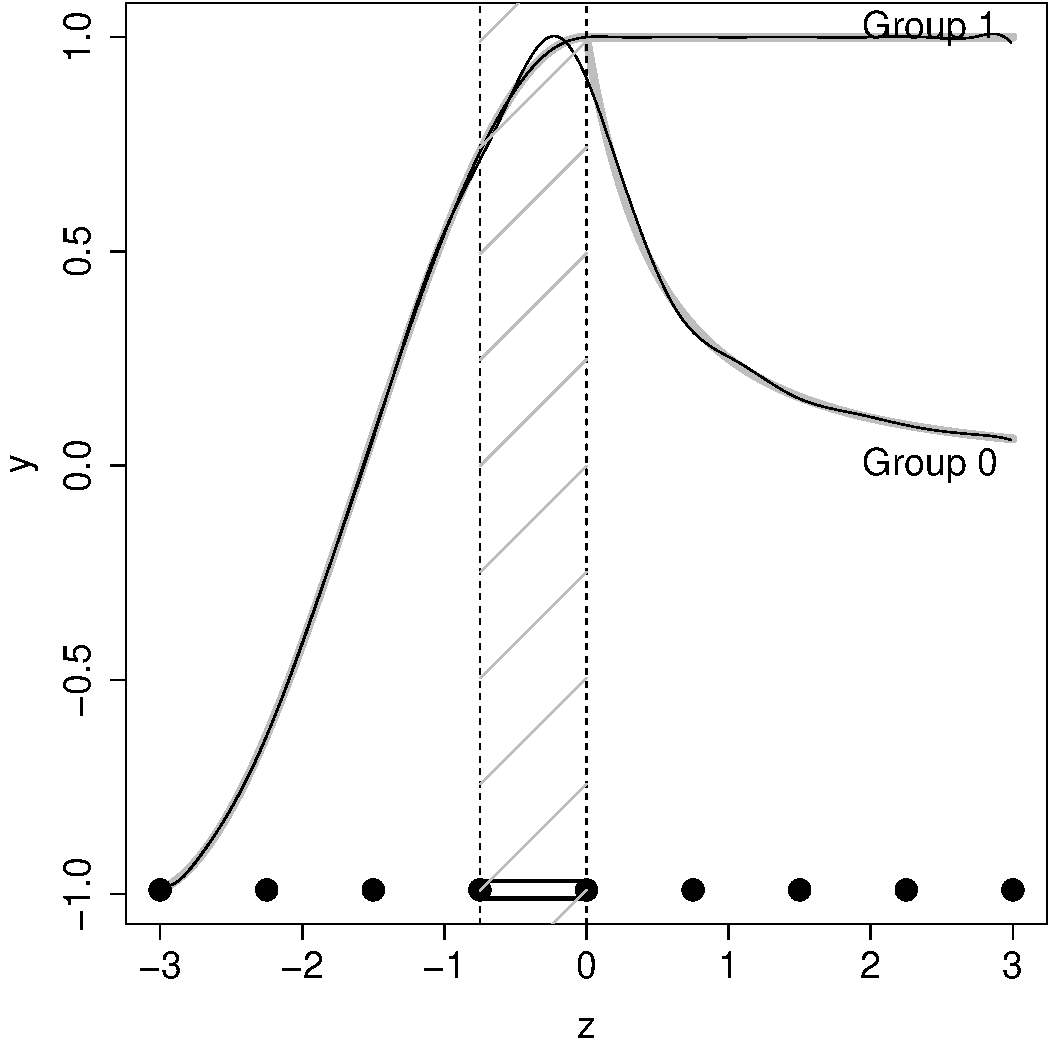
\includegraphics[width=0.48\textwidth, height=0.42\textwidth]{../../figs/bspline_fit_cubic.pdf} &
%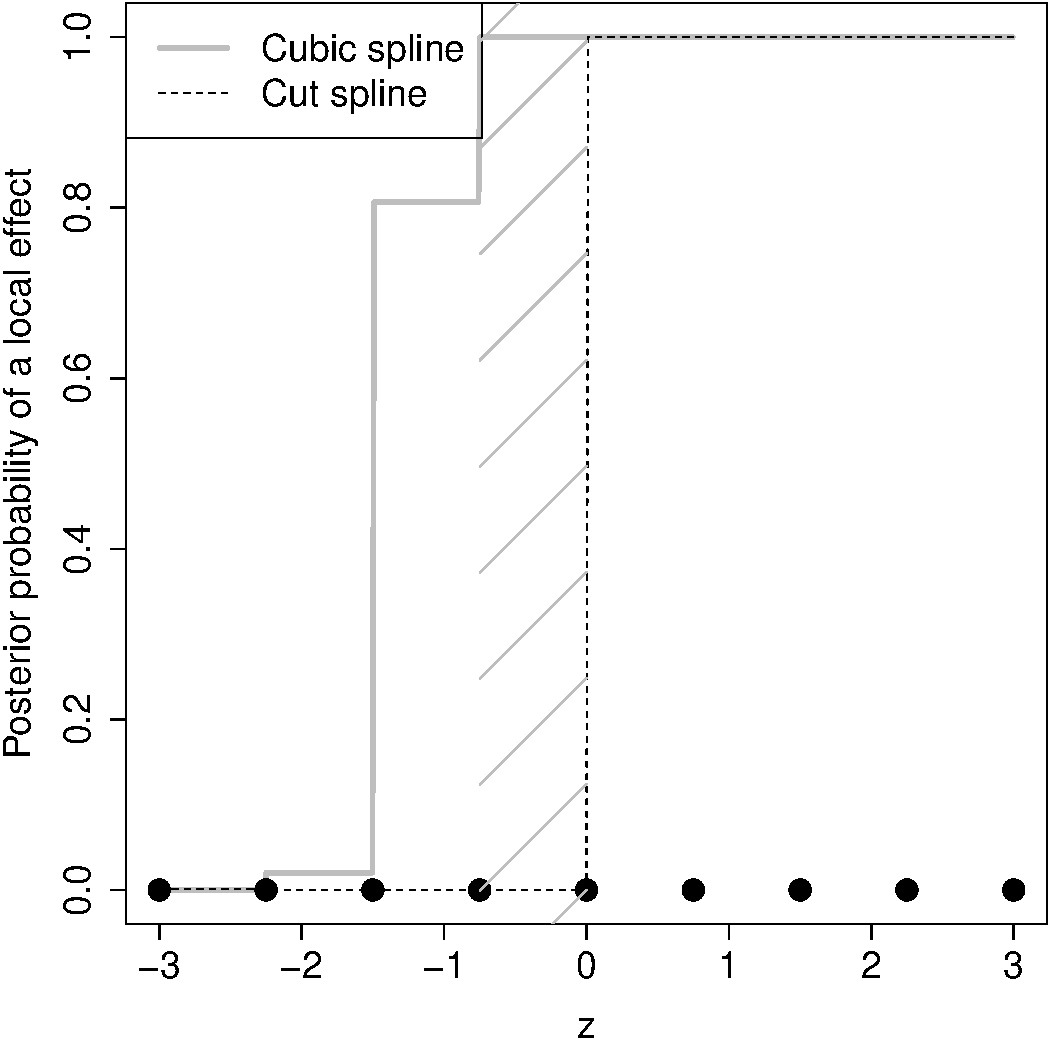
\includegraphics[width=0.48\textwidth, height=0.42\textwidth]{../../figs/bspline_cubic_pp.pdf} \\
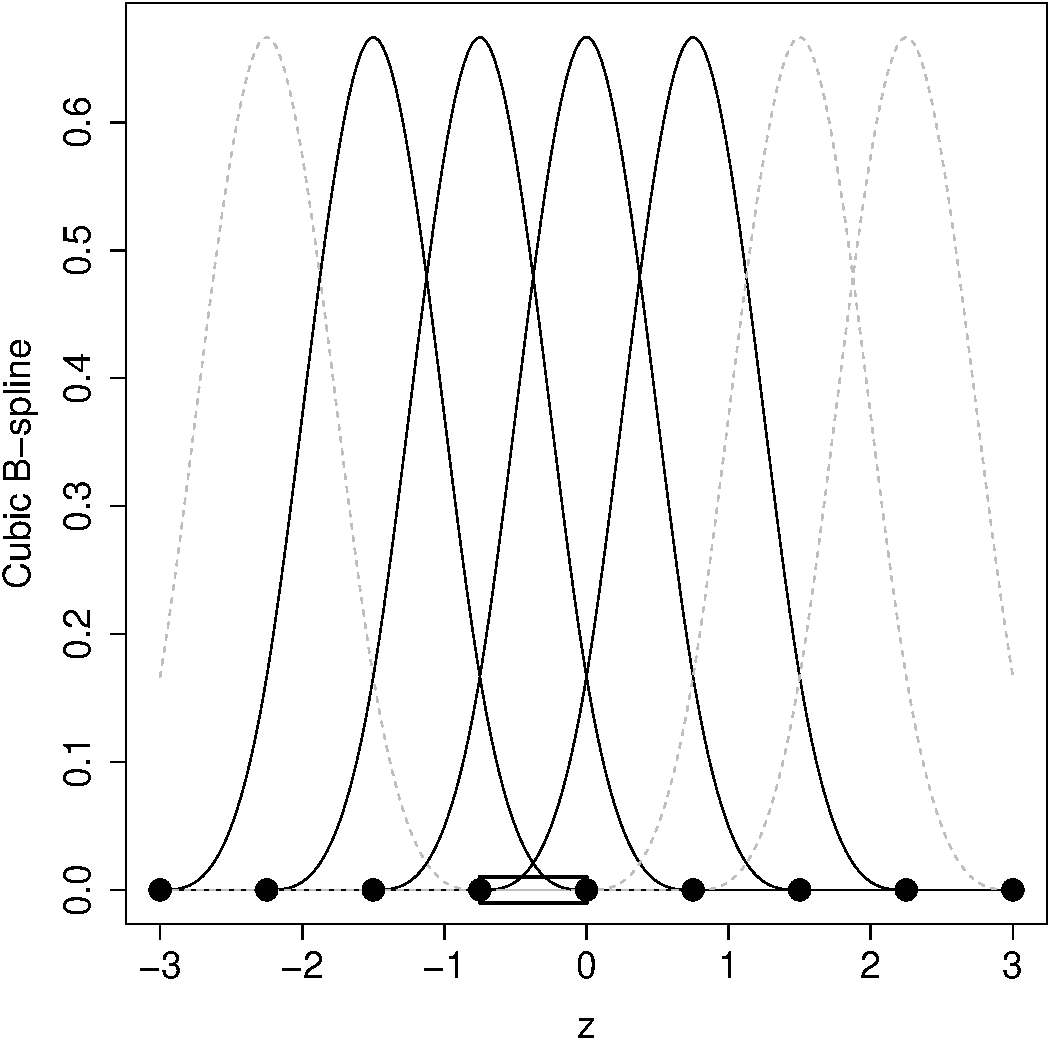
\includegraphics[width=0.48\textwidth, height=0.42\textwidth]{figs/bspline_cubic.pdf} &
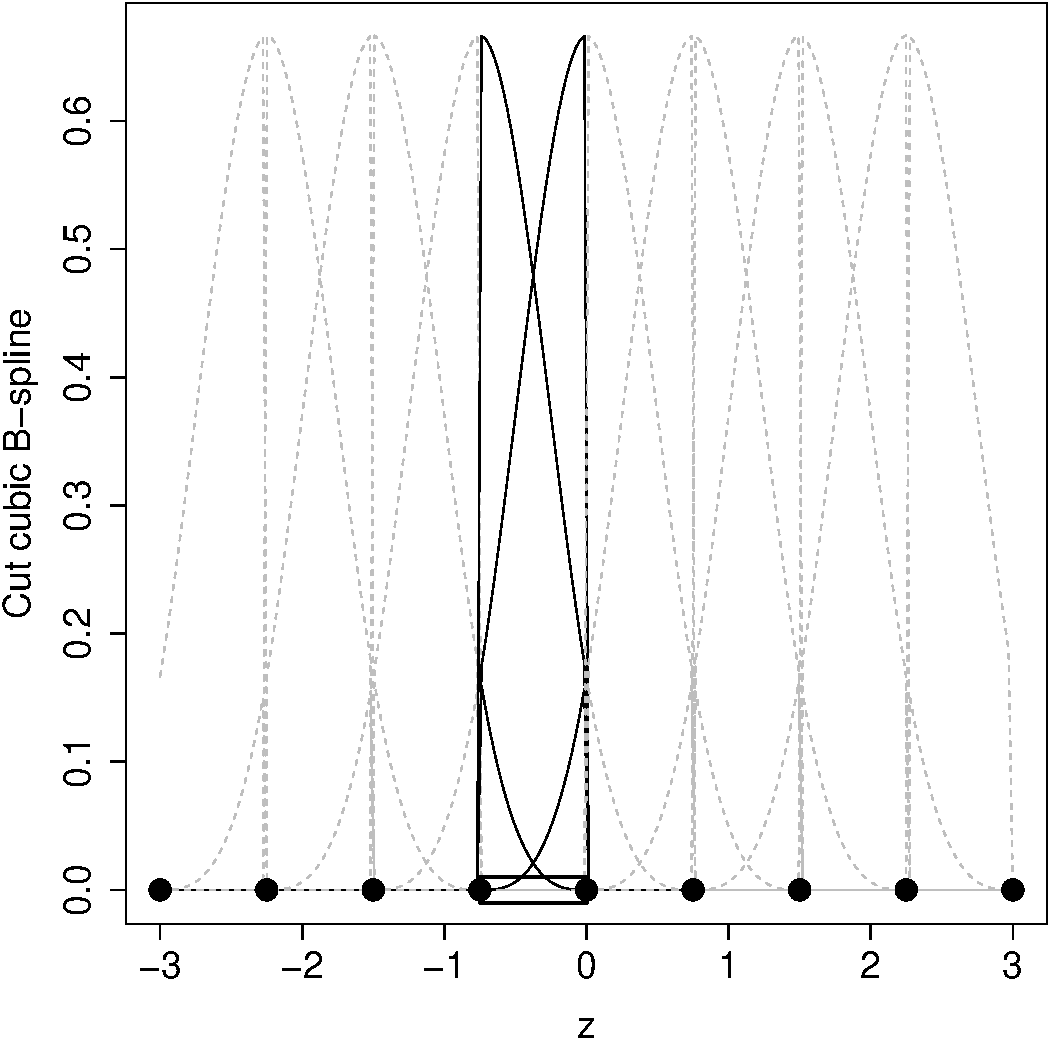
\includegraphics[width=0.48\textwidth, height=0.42\textwidth]{figs/cutspline_cubic.pdf} \\
\end{tabular}
\end{center}
\caption{Cubic B-splines (left) and cut cubic B-splines (right) for the simulated illustration in Figure \ref{fig:splinefit}.
%Top: true group means and their cubic B-spline projections (left), and posterior probability of local group differences for cubic and cut cubic B-splines based on $n=100$ (right).
%Bottom: basis functions for cubic (left) and the proposed cut cubic (right) splines, with corresponding knots and basis (right).
%{\color{red} M: the figure with the posterior probabilities of local group differences is not super clear}  
}
\label{fig:splinefit_suppl}
\end{figure}


\subsection{Extension of the example in Figure \ref{fig:splinefit}}

\begin{figure}
\begin{center}
\begin{tabular}{cc}
\multicolumn{2}{c}{12 knots for baseline, 8 knots for local tests} \\
$n=1000$ & $n=2000$ \\
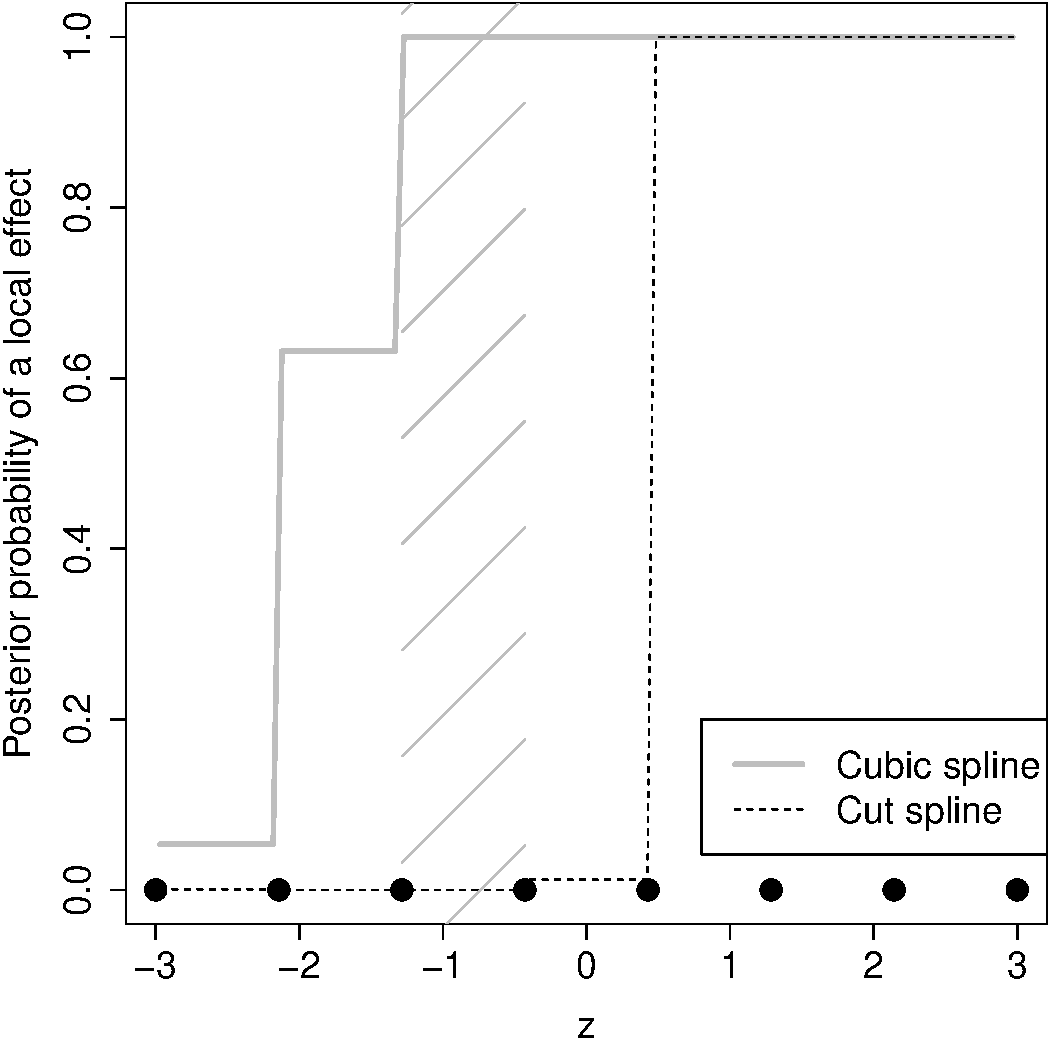
\includegraphics[width=0.48\textwidth, height=0.38\textwidth]{figs/bspline_cubic_pp_8knots.pdf} &
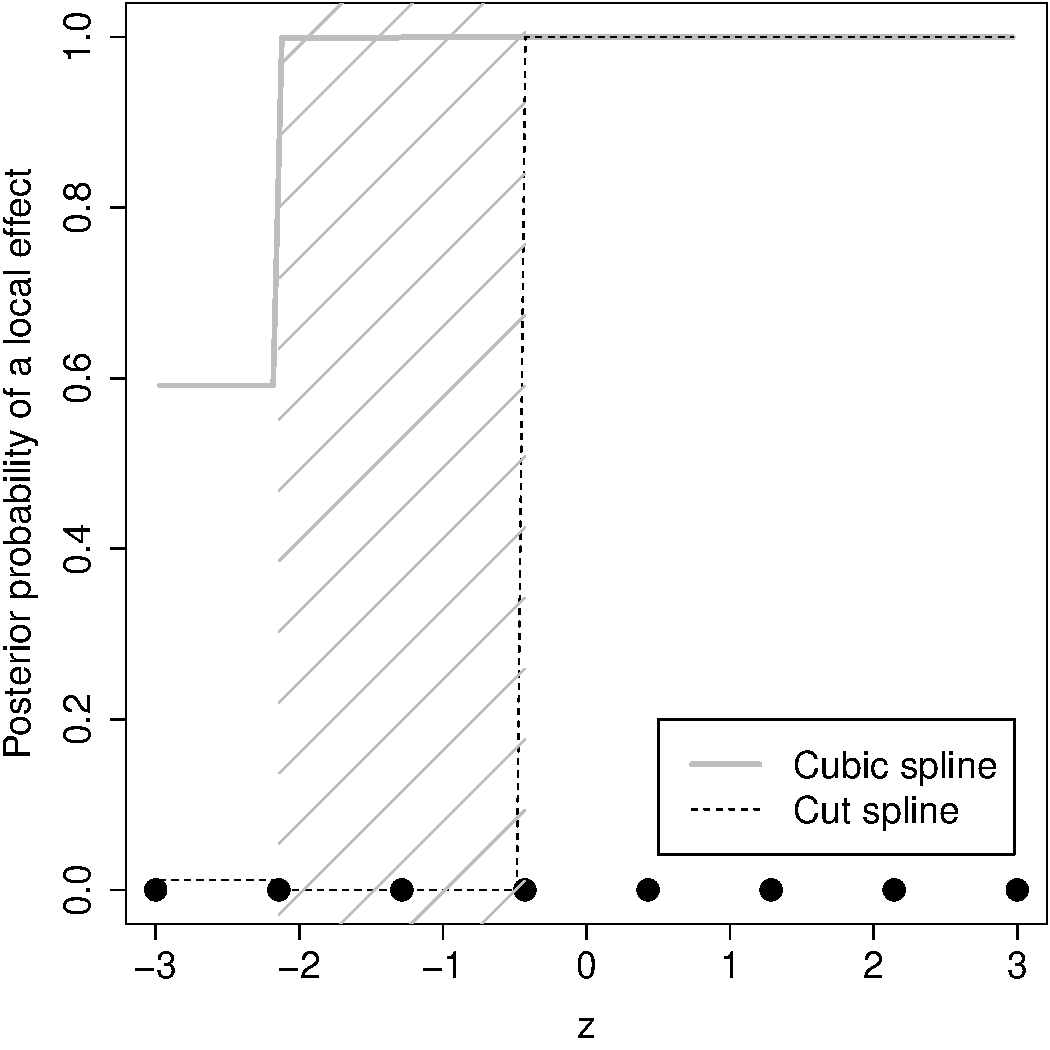
\includegraphics[width=0.48\textwidth, height=0.38\textwidth]{figs/bspline_cubic_pp_8knots_n2000.pdf} \\
\multicolumn{2}{c}{20 knots for baseline, 15 knots for local tests} \\
$n=1000$ & $n=2000$ \\
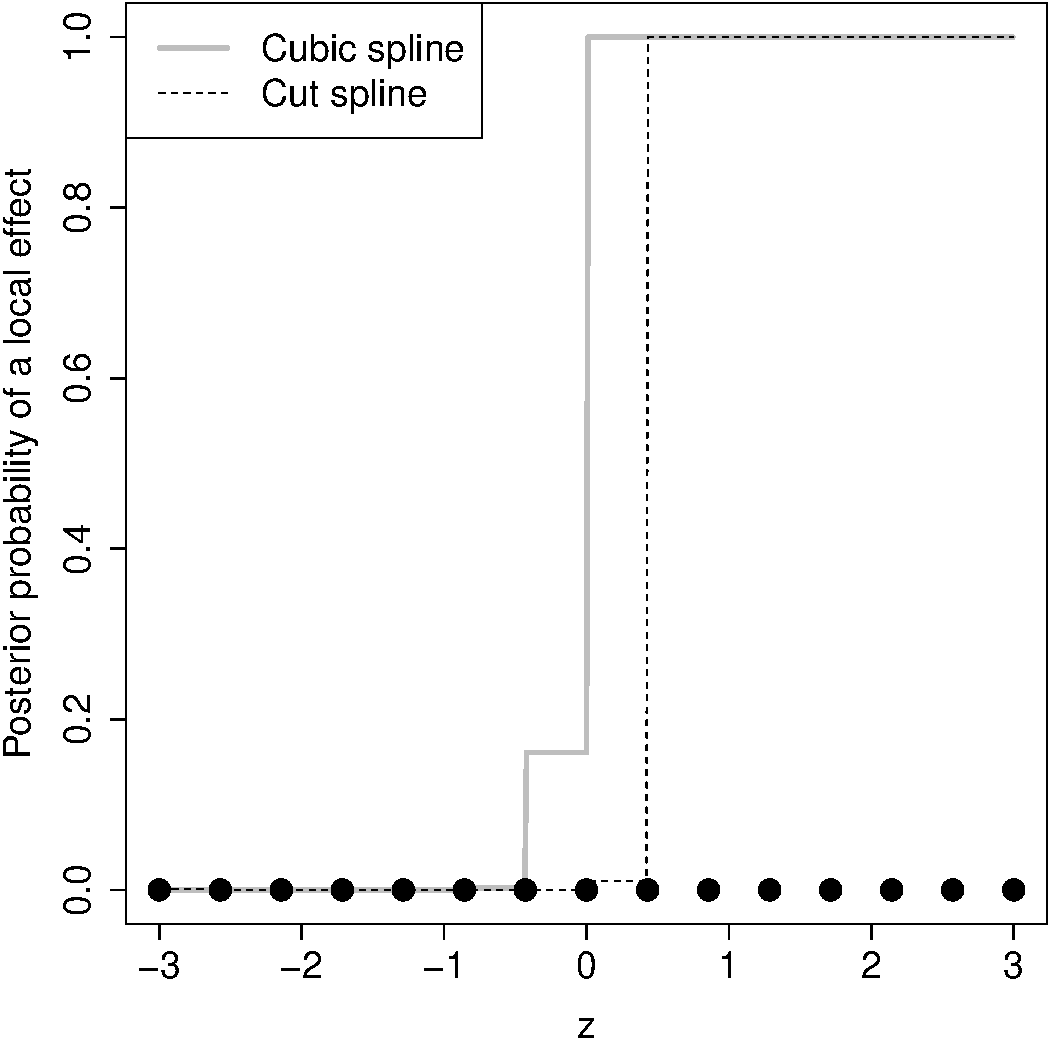
\includegraphics[width=0.48\textwidth, height=0.38\textwidth]{figs/bspline_cubic_pp_15knots.pdf} &
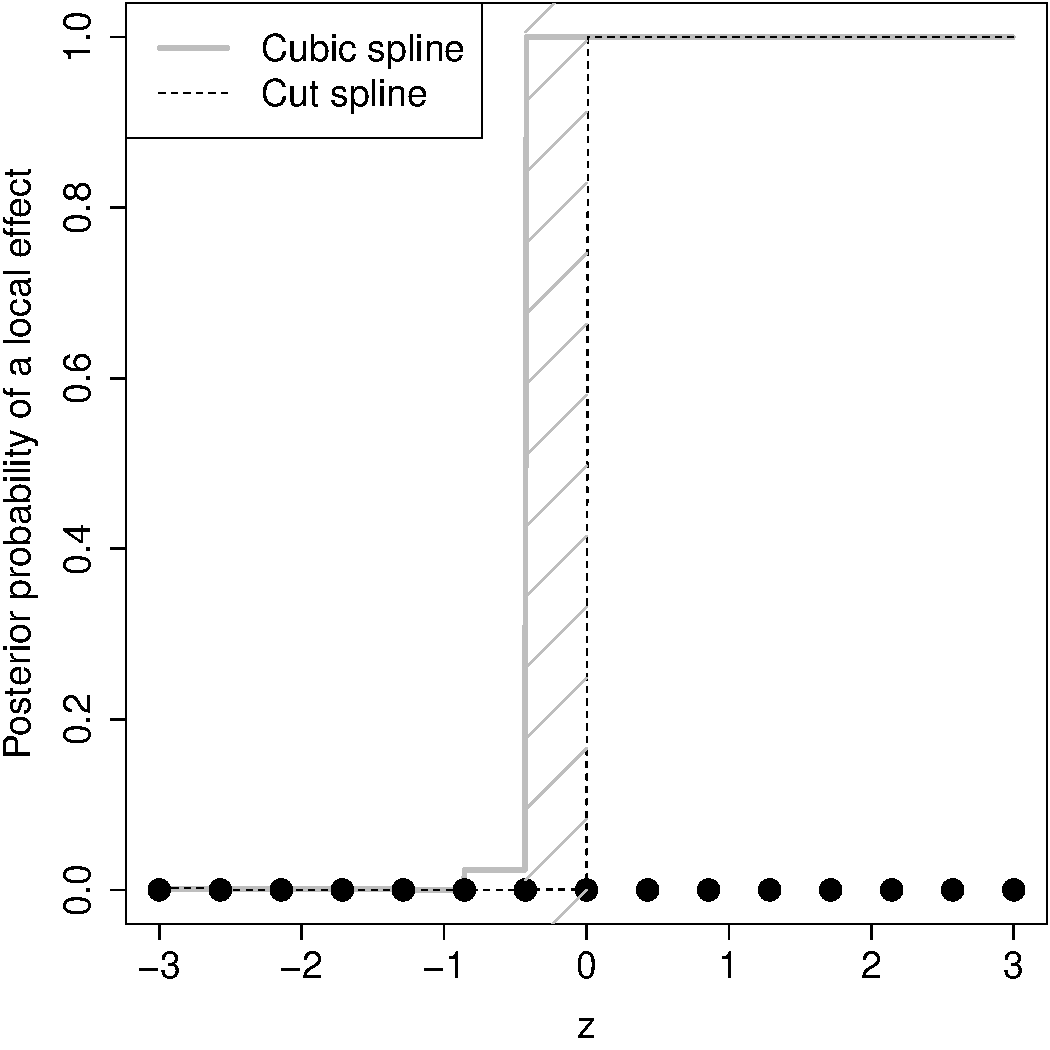
\includegraphics[width=0.48\textwidth, height=0.38\textwidth]{figs/bspline_cubic_pp_15knots_n2000.pdf} \\
\multicolumn{2}{c}{30 knots for baseline, 30 knots for local tests} \\
$n=1000$ & $n=2000$ \\
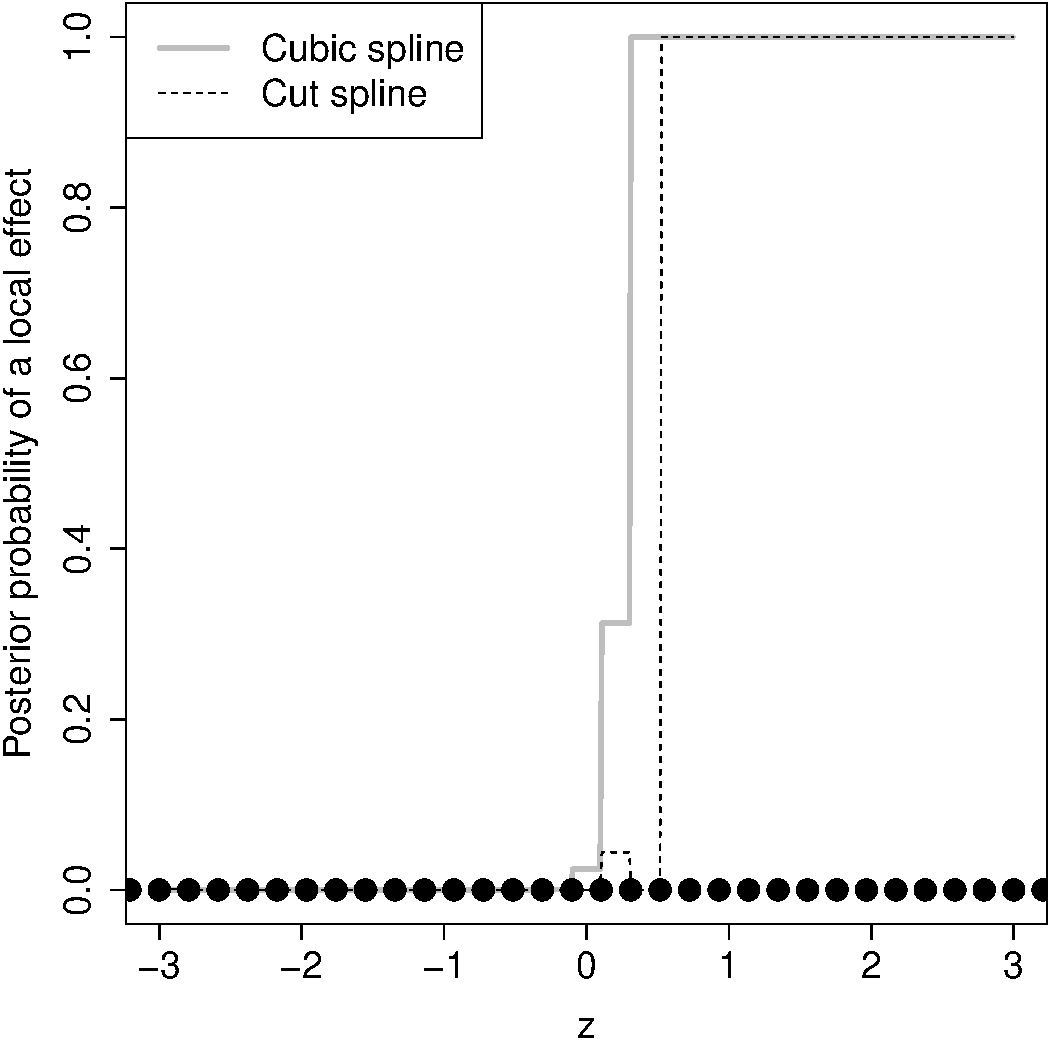
\includegraphics[width=0.48\textwidth, height=0.38\textwidth]{figs/bspline_cubic_pp_30knots.pdf} &
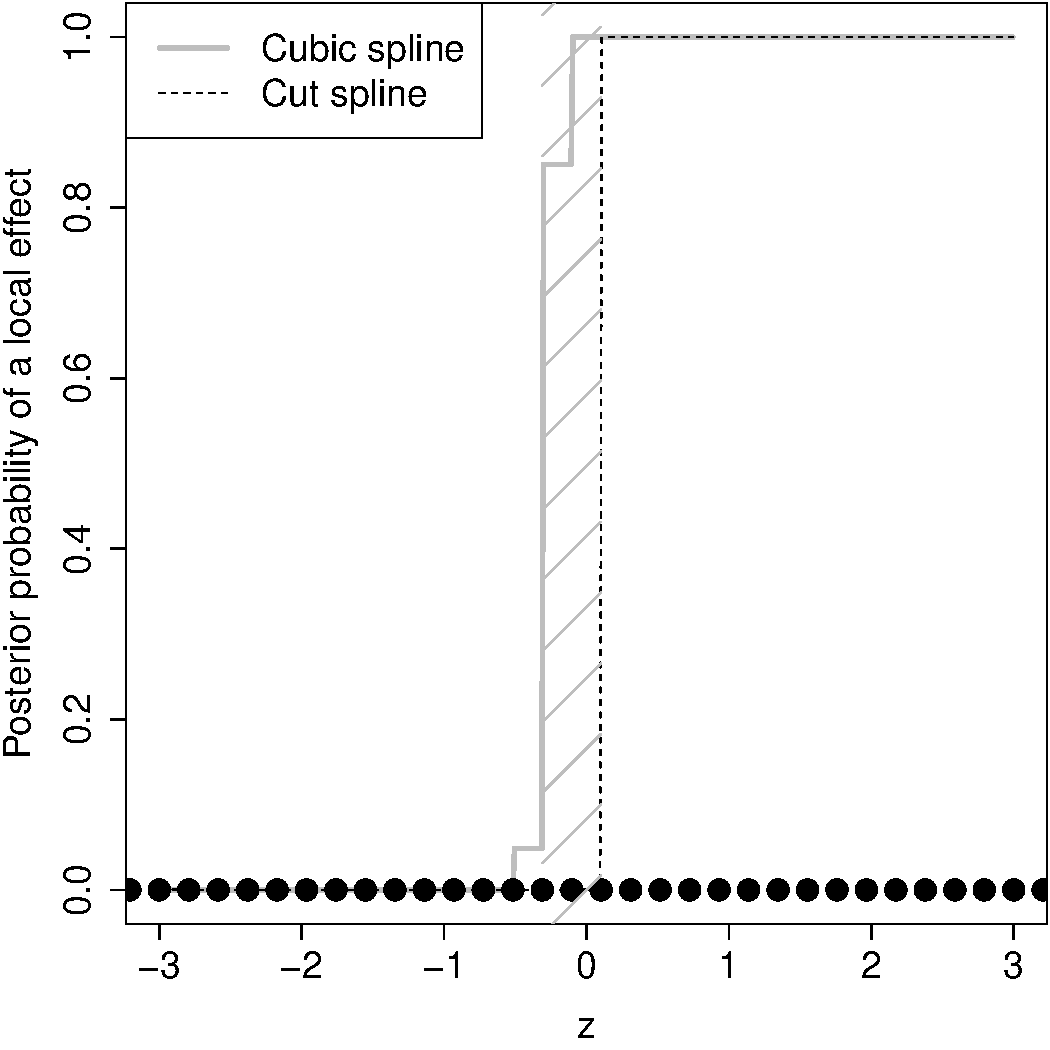
\includegraphics[width=0.48\textwidth, height=0.38\textwidth]{figs/bspline_cubic_pp_30knots_n2000.pdf} \\
\end{tabular}
\end{center}
\caption{Simulated illustration. Posterior probability of local group differences for cubic / cut cubic B-splines varying the knots and $n$. Shaded regions suffer from false positives}
\label{fig:splinefit_varyingknots}
\end{figure}


We extend the top panels in Figure \ref{fig:splinefit}, where one considers different number of knots and sample sizes.
Figure \ref{fig:splinefit_varyingknots} shows posterior probabilities for the presence of local group differences for the same examples as in Figure \ref{fig:splinefit}, but here we vary the number of knots and sample sizes.
The shaded areas indicate regions where there is false positive inflation, i.e. the posterior probability of a local covariate effect in that region is large, but there's truly no effect.
Overall the same phenomenon persists, for larger $n$ the standard B-splines leads to falsely rejecting the null in a neighborhood of $z<0$, whereas the cut B-splines avoid the false positive issue. 
The bottom left panel illustrates how, if the number of knots is too large, the power to detect local differences decreases, in this case for $z \in [0,0.5]$.




\subsection{Simulation with independent errors}
\label{ssec:simulation_iid}

We outline supplementary results for the simulation study presented in Section \ref{sec:simulation_iid} of the main manuscript.
%Table \ref{tab:simiid} shows type I error and power (across 100 simulations) for the various considered methods.
Figure \ref{fig:simiid} shows the posterior probability (average across 100 simulations) for the presence of a covariate effect as a function of $z$.
Covariate 1 is truly active for $z>0$ and inactive for $z \leq 0$, covariates 2-10 are truly inactive at any $z \in [-3,3]$.


Table \ref{tab:simiid_extra} provide further results regarding our simulation with independent errors, related to using alternative methods to those described in the main paper.
It shows the average proportion of rejected local null hypotheses, separately for covariate 1 (which is truly active for $z>0$) and the other covariates.
Specifically, it considers a Benjamini-Hochberg P-value adjustment from a least-squares fit, a fused LASSO fit based on our degree 0 cut orthogonal basis, standard (uncut) cubic splines (which, as opposed to our cut orthogonal splines, runs into false positive issues) and a generalized additive model in mgcv with twice the default knots (24 knots).
%For our methodology, we show the results from using either a Gaussian shrinkage prior on the coefficients (diagonal covariance) or an ICAR+ prior. Local null hypotheses are rejected when $P(\beta_j(z) \neq 0 \mid y) > 0.95$.
%We also considered VC-BART, generalized additive models from R package mgcv (with the default 12 knots and also with 24 knots), applying the fused LASSO to our cut orthogonal basis, and applying Benjamini-Hochberg P-value adjustment.

%The results for the Gaussian shrinkage and ICAR+ priors were very similar. Both controlled the type I error below the 0.01 level, and exhibited a high power to detect truly non-zero local effects ($\beta_1(z) \neq 0$, for $z>0$).
%VC-BART and the additive model showed a competitive performance, albeit the type I error was above 0.05 in several instances.
Benjamini-Hochberg adjusted P-values were too conservative, exhibiting very low power for $n=100$, whereas the fused LASSO was overly liberal, with type I errors that were above 0.1 even when $n=1000$.
The uncut cubic splines and GAM resulted in an inflated type I error for covariate 1, for $z \in (0,1]$.


Table \ref{tab:simiid_mse} displays the root mean squared error for the various considered methods.


\begin{table}
\begin{center}
\begin{tabular}{ccccccccc} %\hline
\multicolumn{9}{c}{$n=100$} \\ %\hline
& \multicolumn{4}{c}{Covariate 1} & \multicolumn{4}{c}{Covariates 2-10} \\ %\hline
 Region          & BH  &  Fused       & Cubic       & GAM          & BH    &  Fused        & Cubic & GAM \\ 
                 &     &  LASSO       & uncut       & 24 knots   &       &  LASSO        & uncut & 24 knots \\ 
$z \in $ (-3,-2] & 0   &  0.69$^{**}$ &     0        &  0.04        & 0     &  0.35 $^{**}$ & 0     &  0.04 \\ 
$z \in $ (-2,-1] & 0   &  0.89$^{**}$ &     0        &  0.03        & 0     &  0.52 $^{**}$ & 0     &  0.04 \\ 
$z \in $  (-1,0] & 0   &  0.82$^{**}$ &     1$^{**}$ &  0.28$^{**}$  & 0     &  0.56$^{**}$  &  0     &  0.05 \\ 
$z \in $   (0,1] & 0.01&  0.91$^{**}$ &     1        &  0.79        & 0.004 &  0.50 $^{**}$ & 0     &   0.05\\ 
$z \in $   (1,2] & 0   &  0.89$^{**}$ &     1        &  0.99        & 0     &  0.21 $^{**}$ & 0     &   0.05\\ 
$z \in $   (2,3] & 0   &  0.95$^{**}$ &     1        &  0.94        & 0     &  0.52 $^{**}$ & 0     &  0.04 \\ 
%\hline
\multicolumn{9}{c}{$n=1000$} \\ %\hline
& \multicolumn{4}{c}{Covariate 1} & \multicolumn{4}{c}{Covariates 2-10} \\ %\hline
 Region         & BH   & Fused        & Cubic  & GAM         & BH    &  Fused & Cubic    & GAM  \\ 
                &     &  LASSO        & uncut  & 24 knots  &       &  LASSO & uncut    & 24 knots \\ 
$z \in $(-3,-2] & 0    &  0.22$^{**}$ & 0       &  0.0008     & 0.004 &  0.07 & 0          & 0.006  \\ 
$z \in $(-2,-1] & 0    &  0.13$^{**}$ & 0.01    &  0.0002     & 0.004 &  0    & 0          & 0.006  \\ 
$z \in $ (-1,0] & 0    &  0.12$^{**}$ & 1$^{**}$ &  0.08$^{**}$& 0    &   0.06 &  0          & 0.01  \\ 
$z \in $  (0,1] & 1    &  1          & 1       &  0.95       & 0.006 &  0    & 0          & 0.01 \\ 
$z \in $  (1,2] & 0.515&  1          & 1       &  1          & 0.001 &  0.05 & 0          & 0.01   \\ 
$z \in $  (2,3] & 1    &  1          & 1       &  1          & 0.002 &  0    & 0          & 0.01  \\ 
%\hline
\end{tabular}
\end{center}
\caption{Independent errors simulation. Proportion of rejected null hypothesis for several methods.
For covariate 1 and $z>0$,  this proportion is the statistical power; otherwise, it is the type I error. ** indicates a type I error $> 0.05$.
The methods are applying Benjamini-Hochberg P-value adjustment
and fused LASSO to our degree 0 cut splines,
using uncut cubic splines in our Bayesian framework, and a GAM with 24 knots.
For fused LASSO the tuning parameters are set to minimize the extended Bayesian information criterion, further only estimates above 0.1 in absolute value are reported as significant}
\label{tab:simiid_extra}
\end{table}


\begin{figure}
\begin{center}
\begin{tabular}{cc}
Average $P(\beta_j(z) \neq 0 \mid y)$ & Proportion of rejected null hypotheses \\
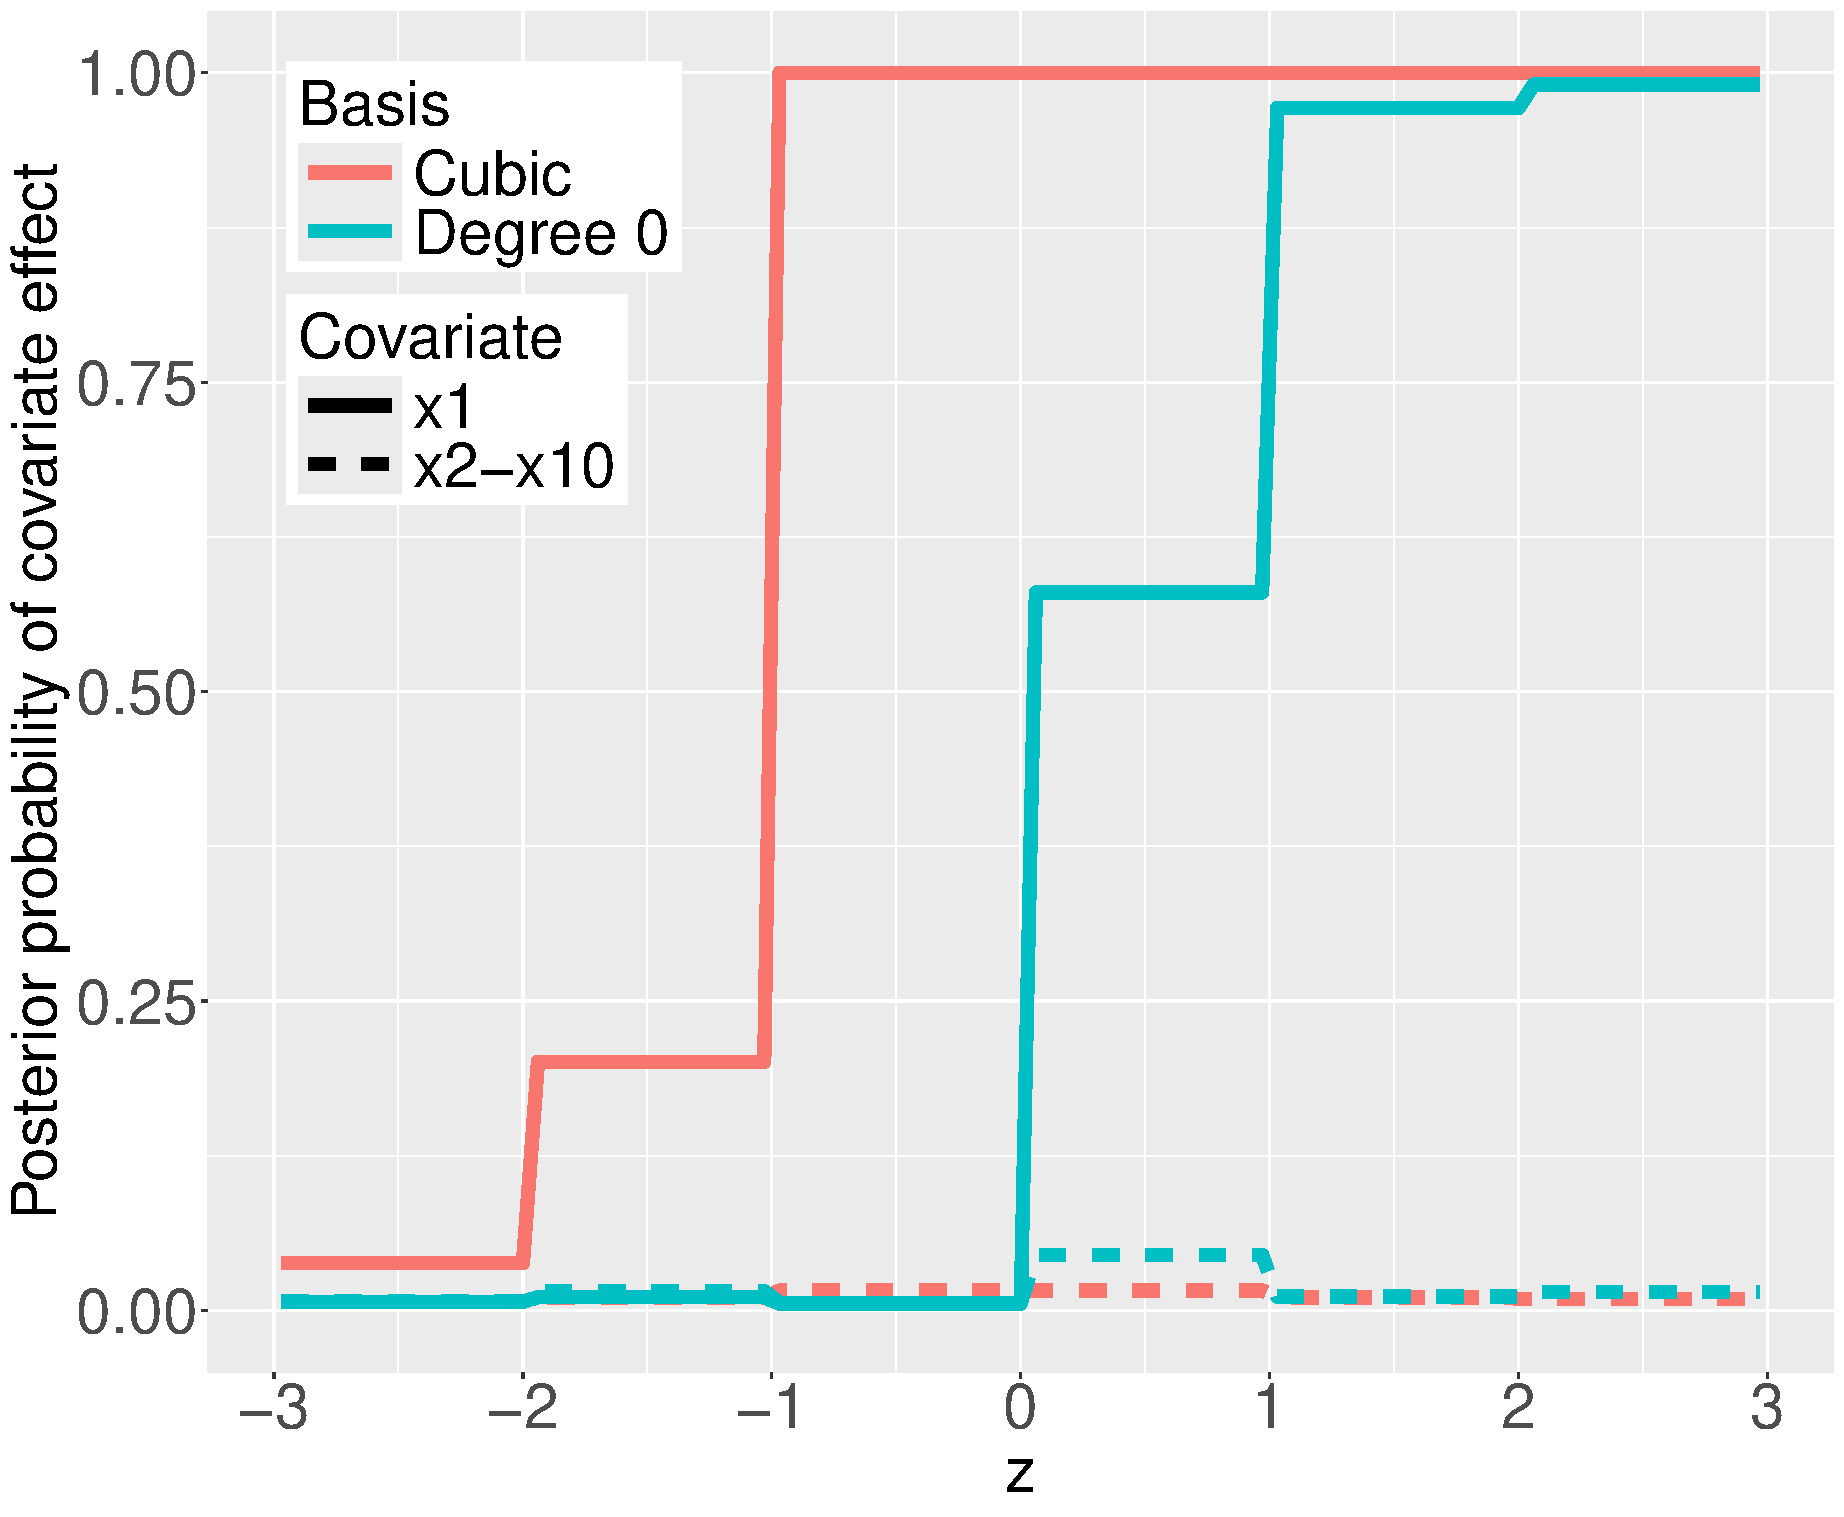
\includegraphics[width=0.5\textwidth]{figs/simiid_pp_n100.pdf} &
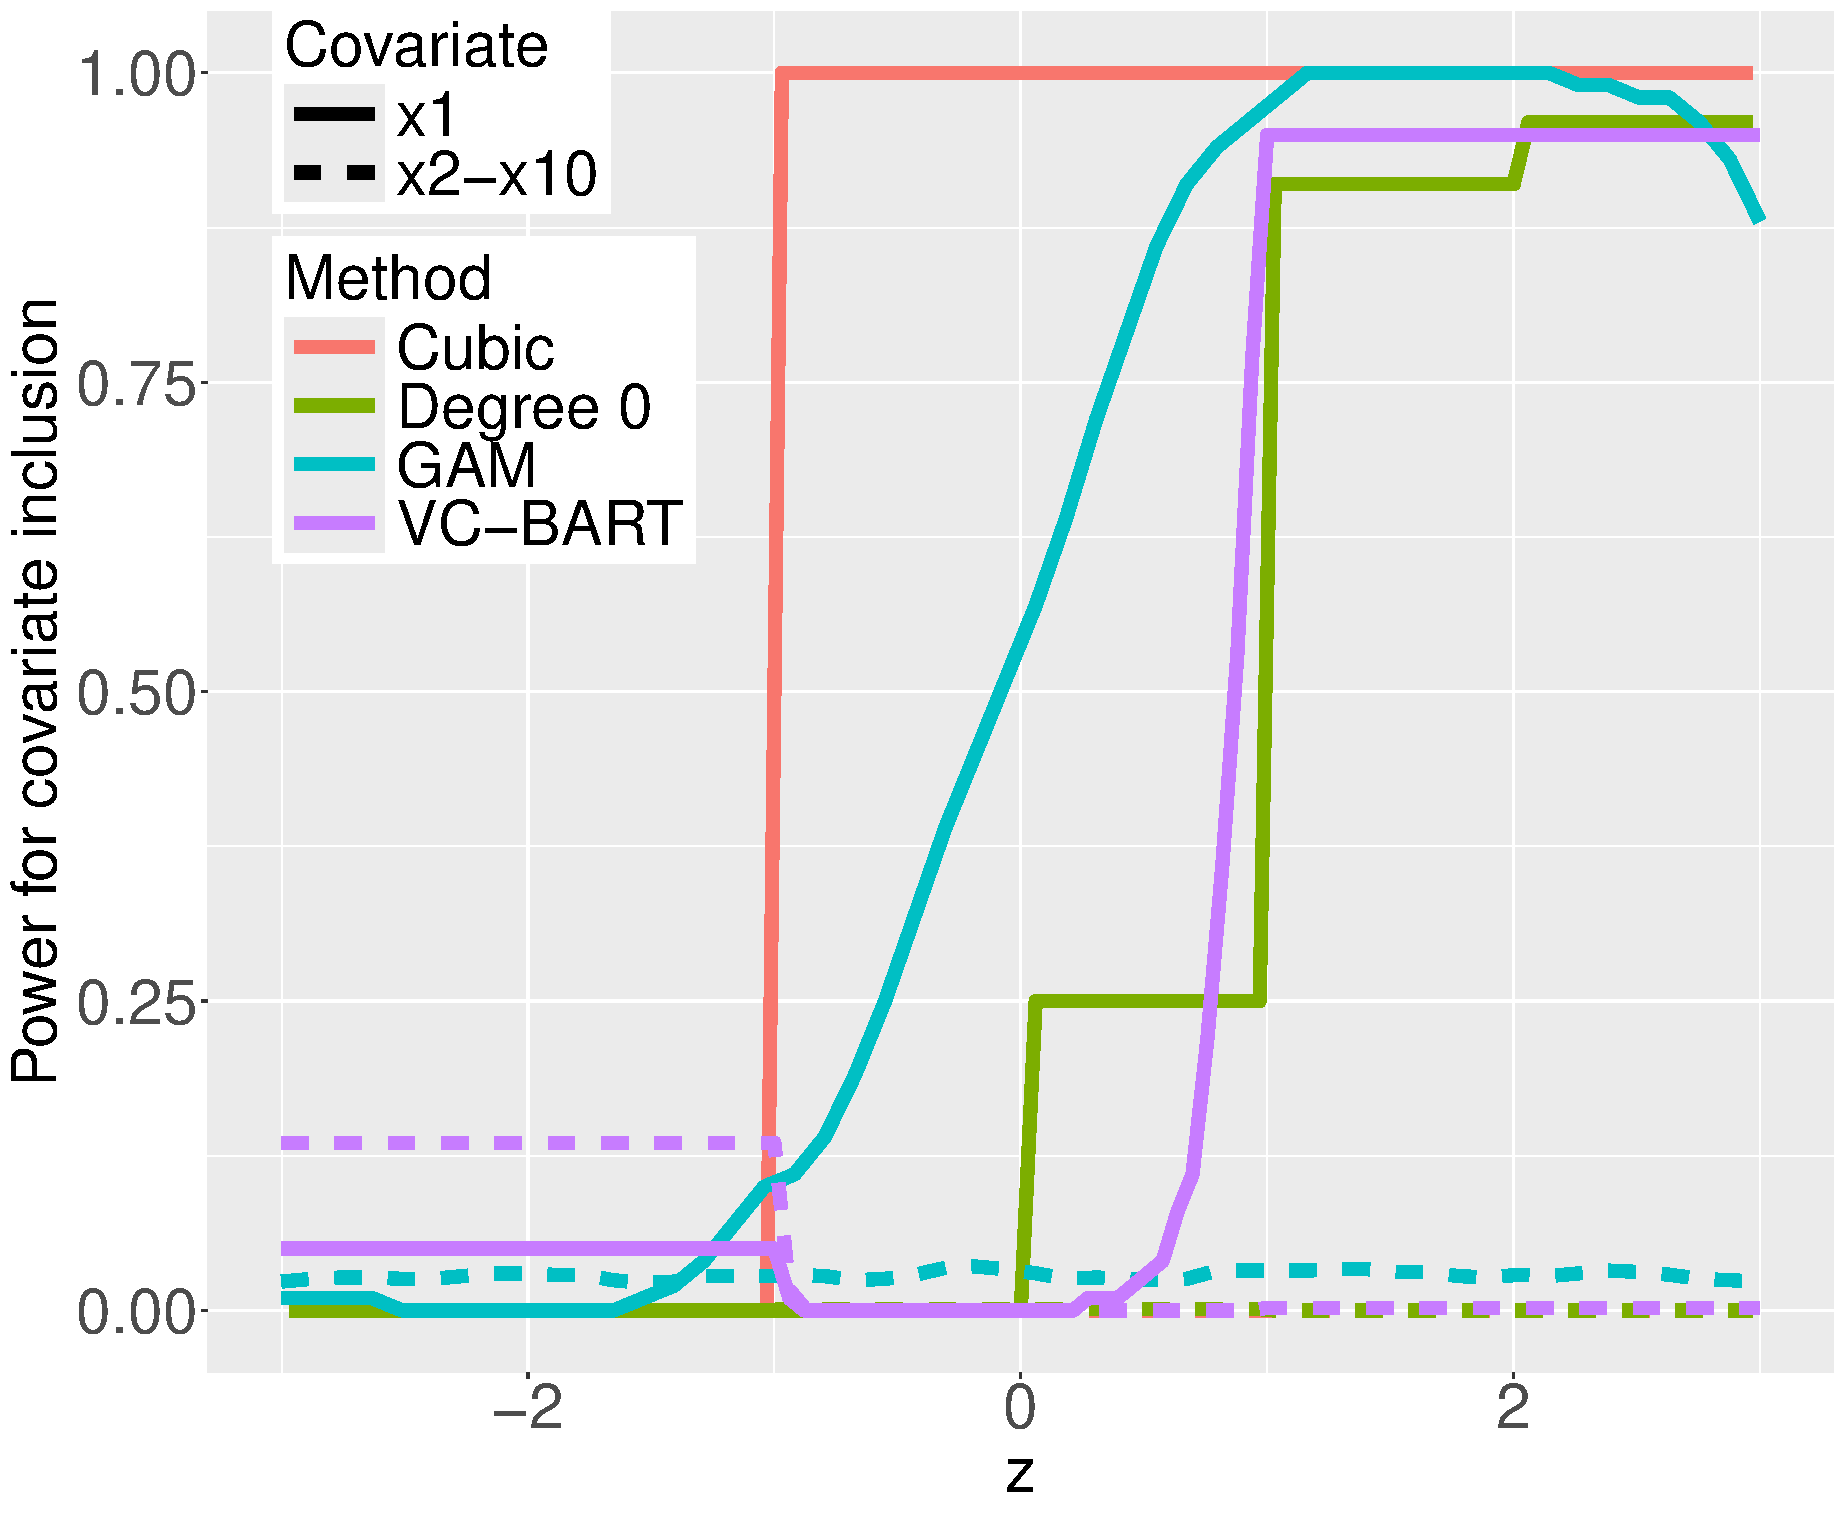
\includegraphics[width=0.5\textwidth]{figs/simiid_pow_n100.pdf} \\
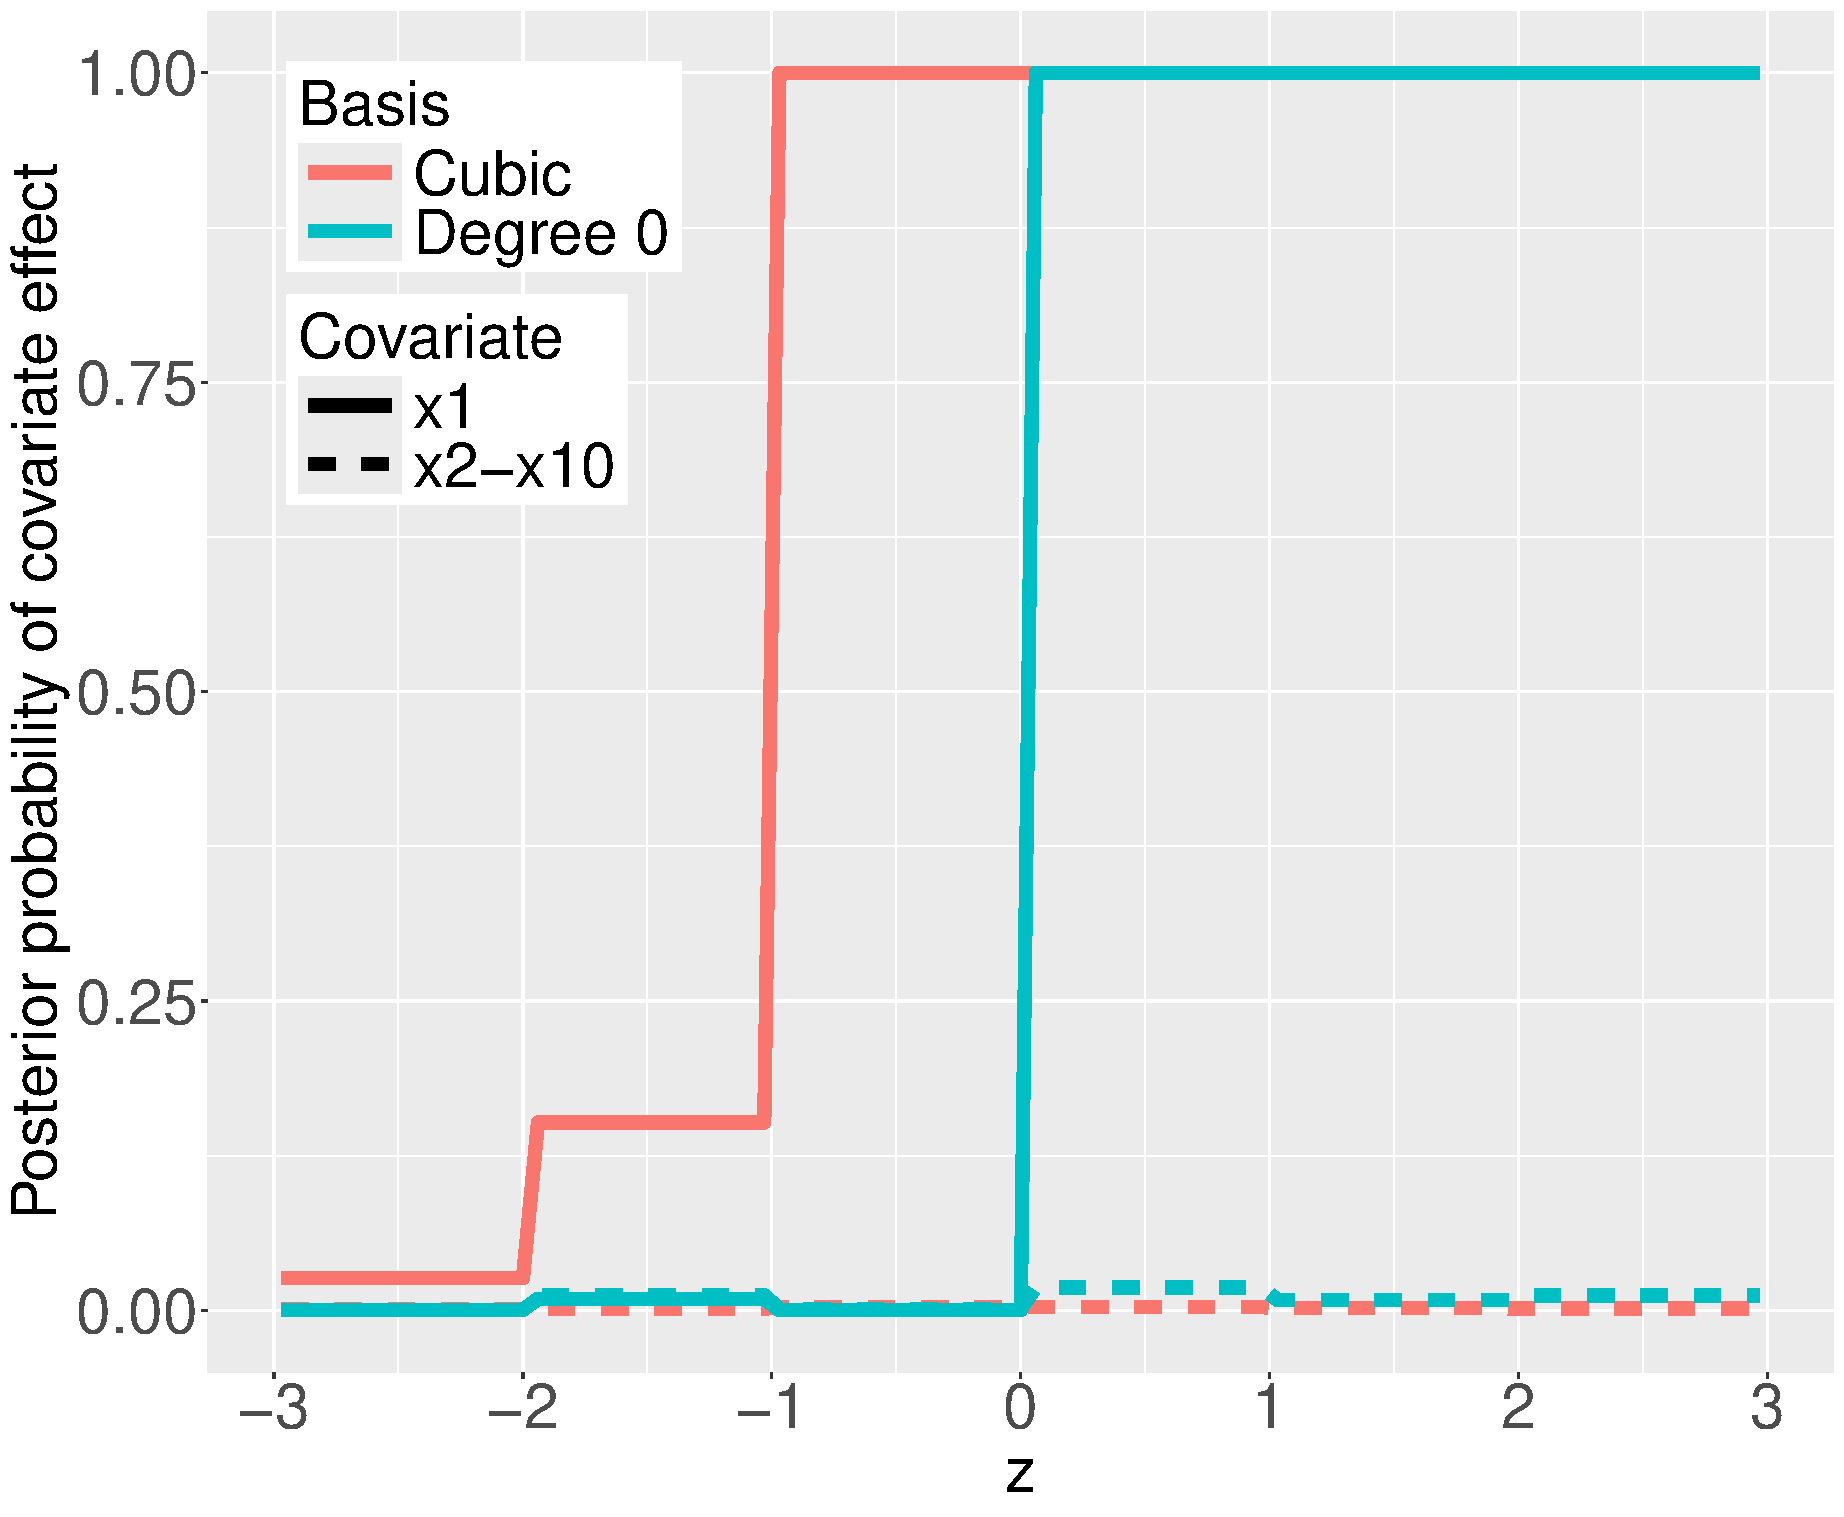
\includegraphics[width=0.5\textwidth]{figs/simiid_pp_n1000.pdf} &
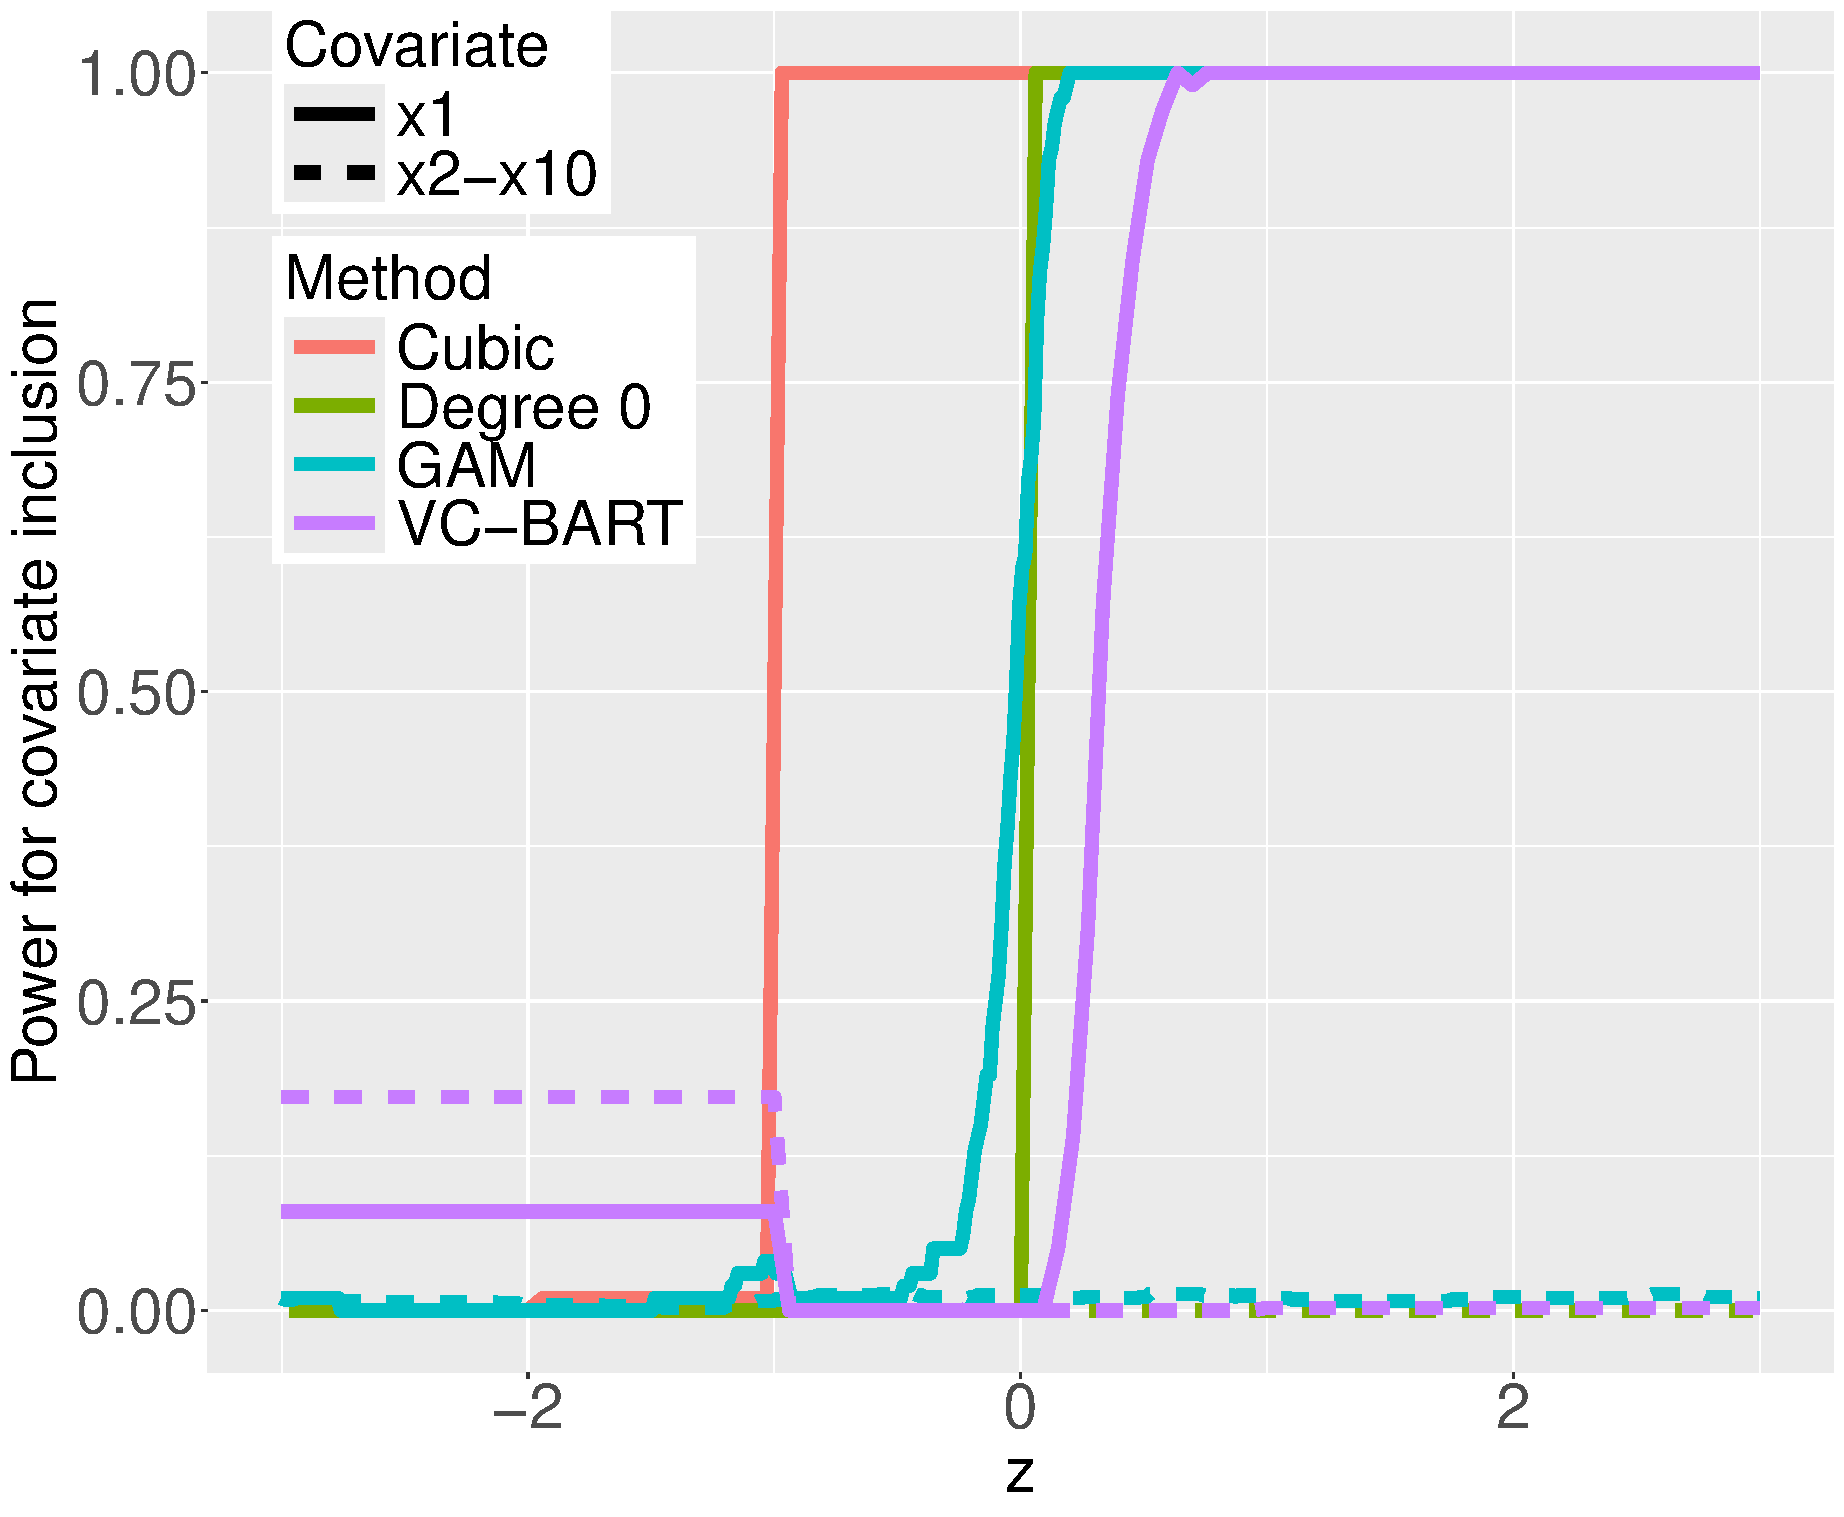
\includegraphics[width=0.5\textwidth]{figs/simiid_pow_n1000.pdf}
\end{tabular}
\end{center}
\caption{Independent errors simulation. Posterior probability of local null test and proportion of rejected null hypotheses. Top: $n=100$. Bottom: $n=1,000$}
\label{fig:simiid}
\end{figure}


\begin{table}
\begin{center}
\begin{tabular}{lcccccc}  %\hline
         & Gaussian &  ICAR+ & Cubic    & VC-BART & GAM        & GAM \\ 
         & prior    &  prior & B-splines&         & 12 knots & 24 knots\\   %\hline
n=100    & 0.173    &  0.166 & 0.168    & 0.297   & 0.159      & 0.173  \\ 
n=1000   & 0.063    &  0.063 & 0.078    & 0.285   & 0.055      & 0.058 \\ 
   %\hline
\end{tabular}
\end{center}
\caption{Independent errors simulation. Root Mean Squared Error $E_F\left[ \hat{E}(y_i) - E_F(y_i) \right]^2$ for 0-degree cut splines, cubic B-splines, VC-BART  and GAM (R package mgcv) with $k=12$ and $k=24$ knots }
\label{tab:simiid_mse}
\end{table}


\begin{table}
\begin{center}
\begin{tabular}{ccc} %\hline
                                                 & $n=100$  & $n=1,000$ \\ %\hline
%David's desktop. NEW mombf version
Gaussian shrinkage prior. Cut degree 0 (1 core)  &   8.5 sec &  5.5 sec  \\ 
Gaussian shrinkage prior. Cut degree 0 (3 cores) &   5.0 sec &  4.0 sec  \\ 
ICAR+ prior. Cut degree 0 (1 core)               &   53.3 sec &  20.3 sec  \\ 
ICAR+ prior. Cut degree 0 (3 cores)              &   31.4 sec &  12.3 sec  \\ 
%David's laptop. NEW mombf version
%Normal shrinkage. Cut degree 0 (1 core)  &  14.9 sec& 9.6 sec \\ 
%Normal shrinkage. Cut degree 0 (3 cores) &   8.8 sec& 7.1 sec \\ 
%ICAR+ prior. Cut degree 0 (1 core)               &   95.1 sec &  36.3 sec  \\ 
%ICAR+ prior. Cut degree 0 (3 cores)              &   56.0 sec &  21.9 sec  \\ 
VCBART          &  69.2 sec  & 7.05 min \\
GAM ($k=12$)             &  1.4 sec  & 4.2 sec\\
GAM ($k=24$)             &  1.3 sec  & 4.2 sec\\
%David's desktop. PREVIOUS mombf version (no fast Cholesky updates)
%Cut degree 0 (1 core)  &  33.6 sec & 27.6sec \\ 
%Cut degree 0 (3 cores) &  22.0 sec& 21.8 sec \\ 
%David's laptop. PREVIOUS mombf version
%Cut degree 0 (1 core)  &  58.2sec & 59.1sec \\ 
%Cut degree 0 (3 cores) &  39.1 sec& 40.8sec \\ 
%VCBART          &  2.2min  & 12.6min \\ 
%\hline
\end{tabular}
\end{center}
\caption{Independent errors simulation. Run times for one simulation on an Ubuntu Linux desktop, 13th Gen Intel core i7 processor, 32Gb RAM}
\label{tab:cputime_simiid}
\end{table}




\subsection{Simulation with independent errors, misaligned knots}
\label{ssec:simulation_iid_misalign}

We extend the simulation results in Section \ref{ssec:simulation_iid} by considering a variation where all the knots in our methodology are misaligned with respect to the true changepoint where $\beta_1(z)$ transitions from zero to non-zero.
Specifically, all settings are equal to those of Section \ref{ssec:simulation_iid}, except that now we set a data-generating $\beta_1(z) = 0$ for $z \leq 0.15$ and $\beta_1(z) \neq 0$ for $z > 0.15$. Recall that $\beta_1(z)$ is the coefficient associated to a binary covariate, hence it defines two group means.
The top panel in Figure \ref{fig:simiid_unaligned} shows this data-generating means for both groups, along with the knots used in our multi-resolution analysis (using our default of 3 resolutions, 
The middle and bottom panels show the average posterior probability $P(\beta_j(z) \neq 0 \mid y)$ and the proportion of rejected local null hypotheses (using a cutoff of $P(\beta_j(z) \neq 0 \mid y) > 0.95$) as a function of $z$.

The results are very similar to those in Section \ref{ssec:simulation_iid}, with some nuisances.
First, note that our specified knots define regions that start at $z=0$ and include the true changepoint $z=0.15$, i.e. regions where $\beta_j(z) \neq 0$ for some $z$ in the region.
Therefore, our approach finds evidence for the existence differences are found within such a region.
That is, our posterior probabilities should be interpreted as there being evidence for differences somewhere in the region.

A second observation is that the average posterior probability and power for $z \in [0,1]$ are slightly lower than in Section \ref{ssec:simulation_iid}, where the knots for two resolutions were aligned with the true changepoint. Intuitively, since truly $\beta_j(z)=0$ for some $z$'s in the region, the statistical power decreases relative to a perfectly aligned region where $\beta_j(z) \neq 0$ for all $z$ in that region.


\begin{figure}
\begin{center}
\begin{tabular}{c}
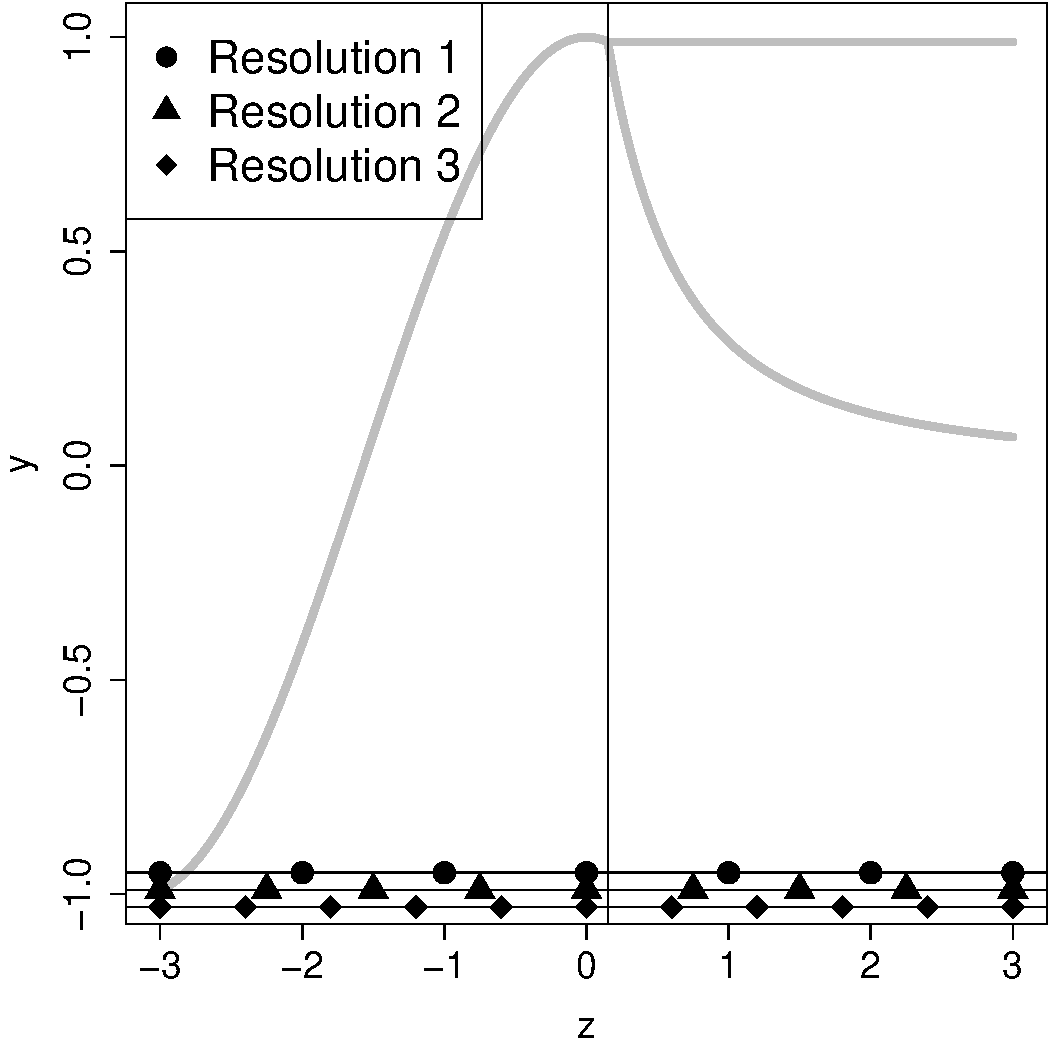
\includegraphics[width=0.5\textwidth,height=0.4\textwidth]{figs/simiid_unaligned.pdf} \\
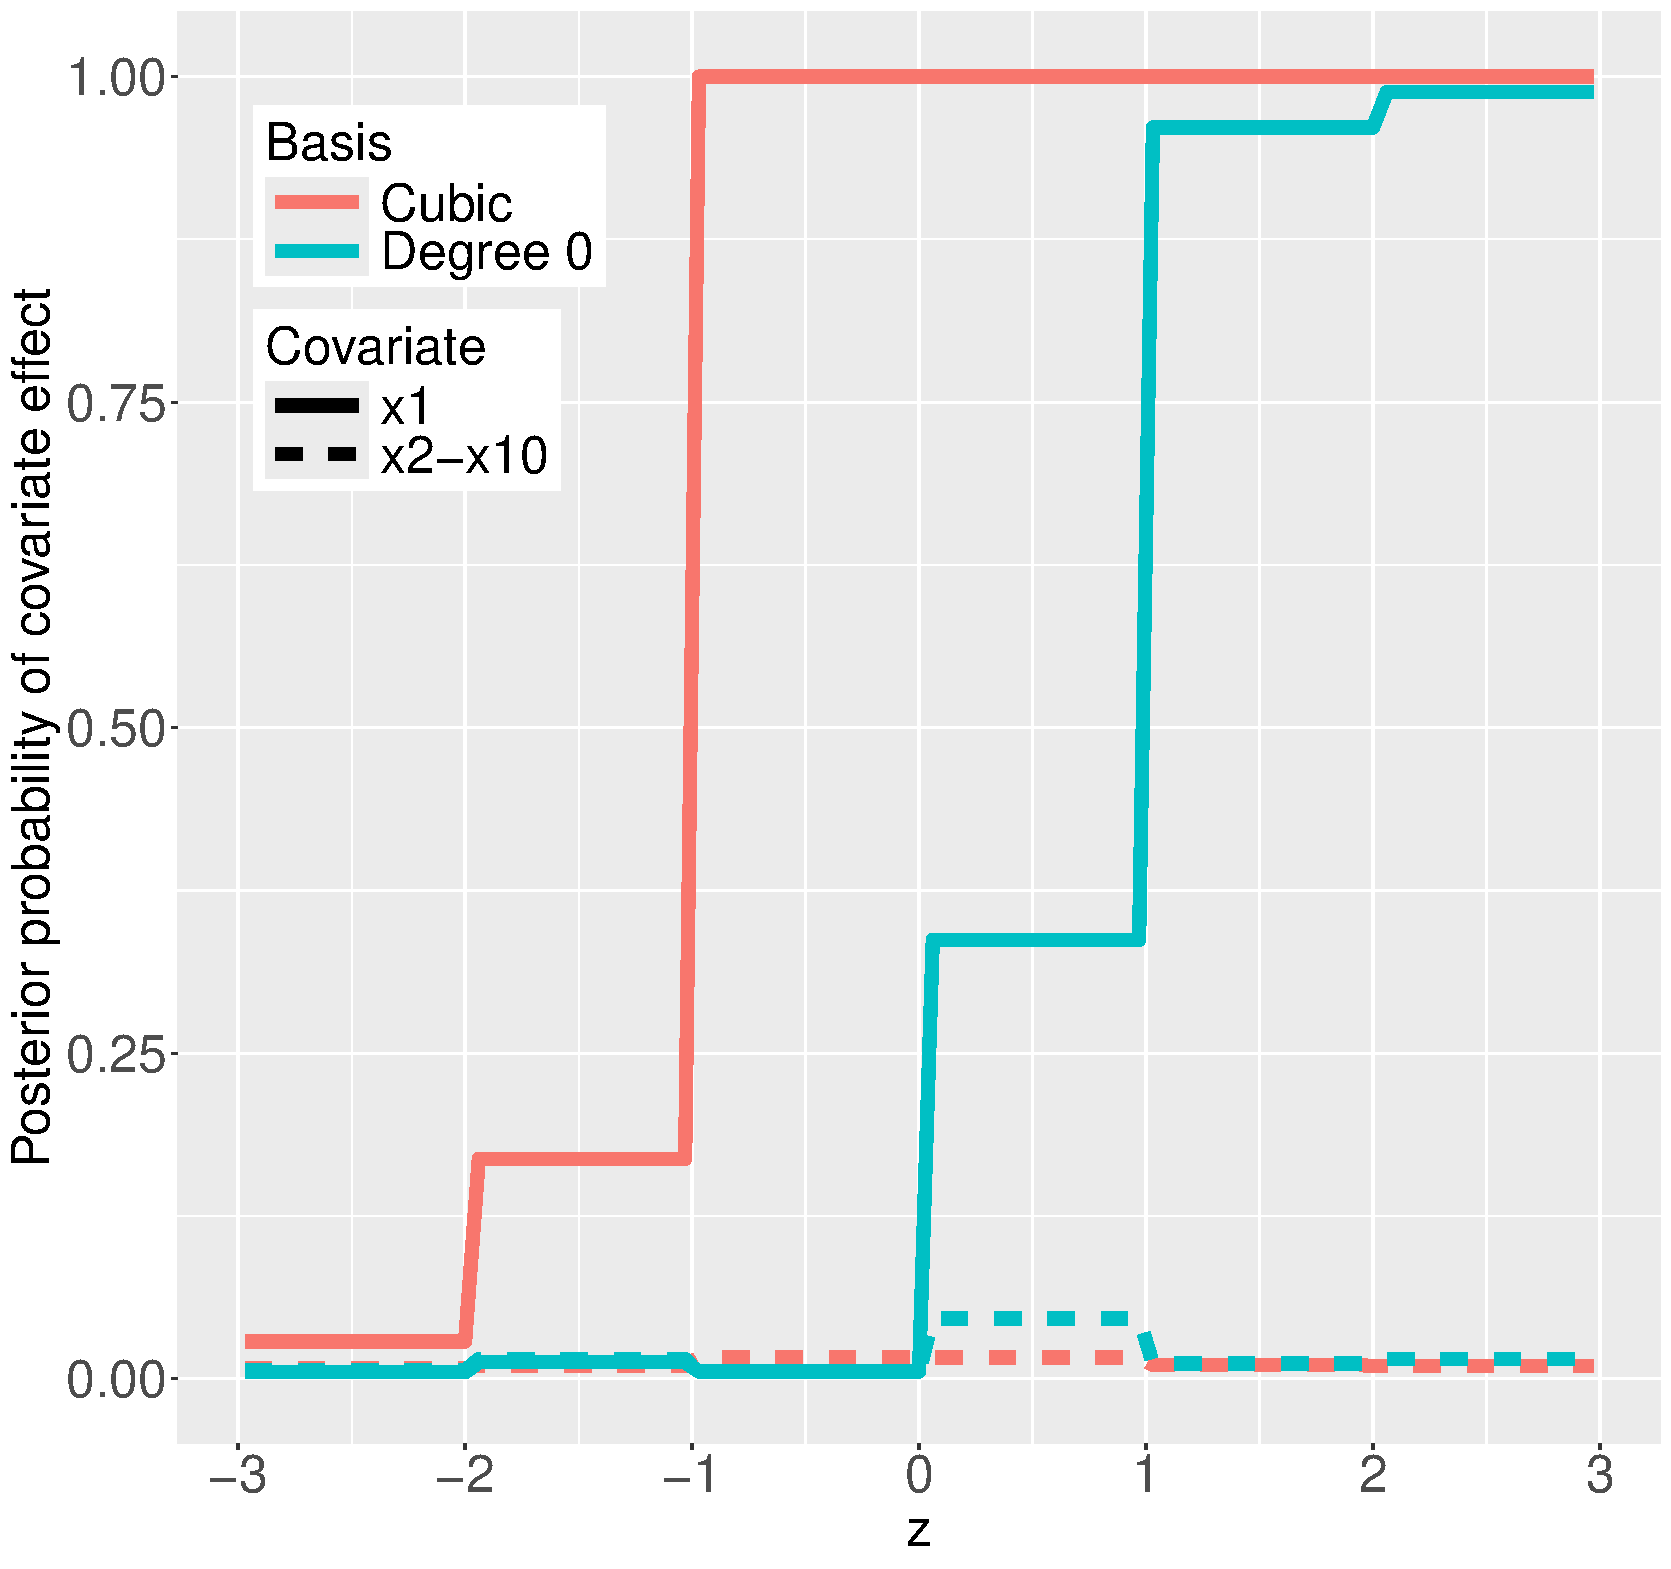
\includegraphics[width=0.5\textwidth,height=0.4\textwidth]{figs/simiid_unaligned_pp_n100.pdf} \\
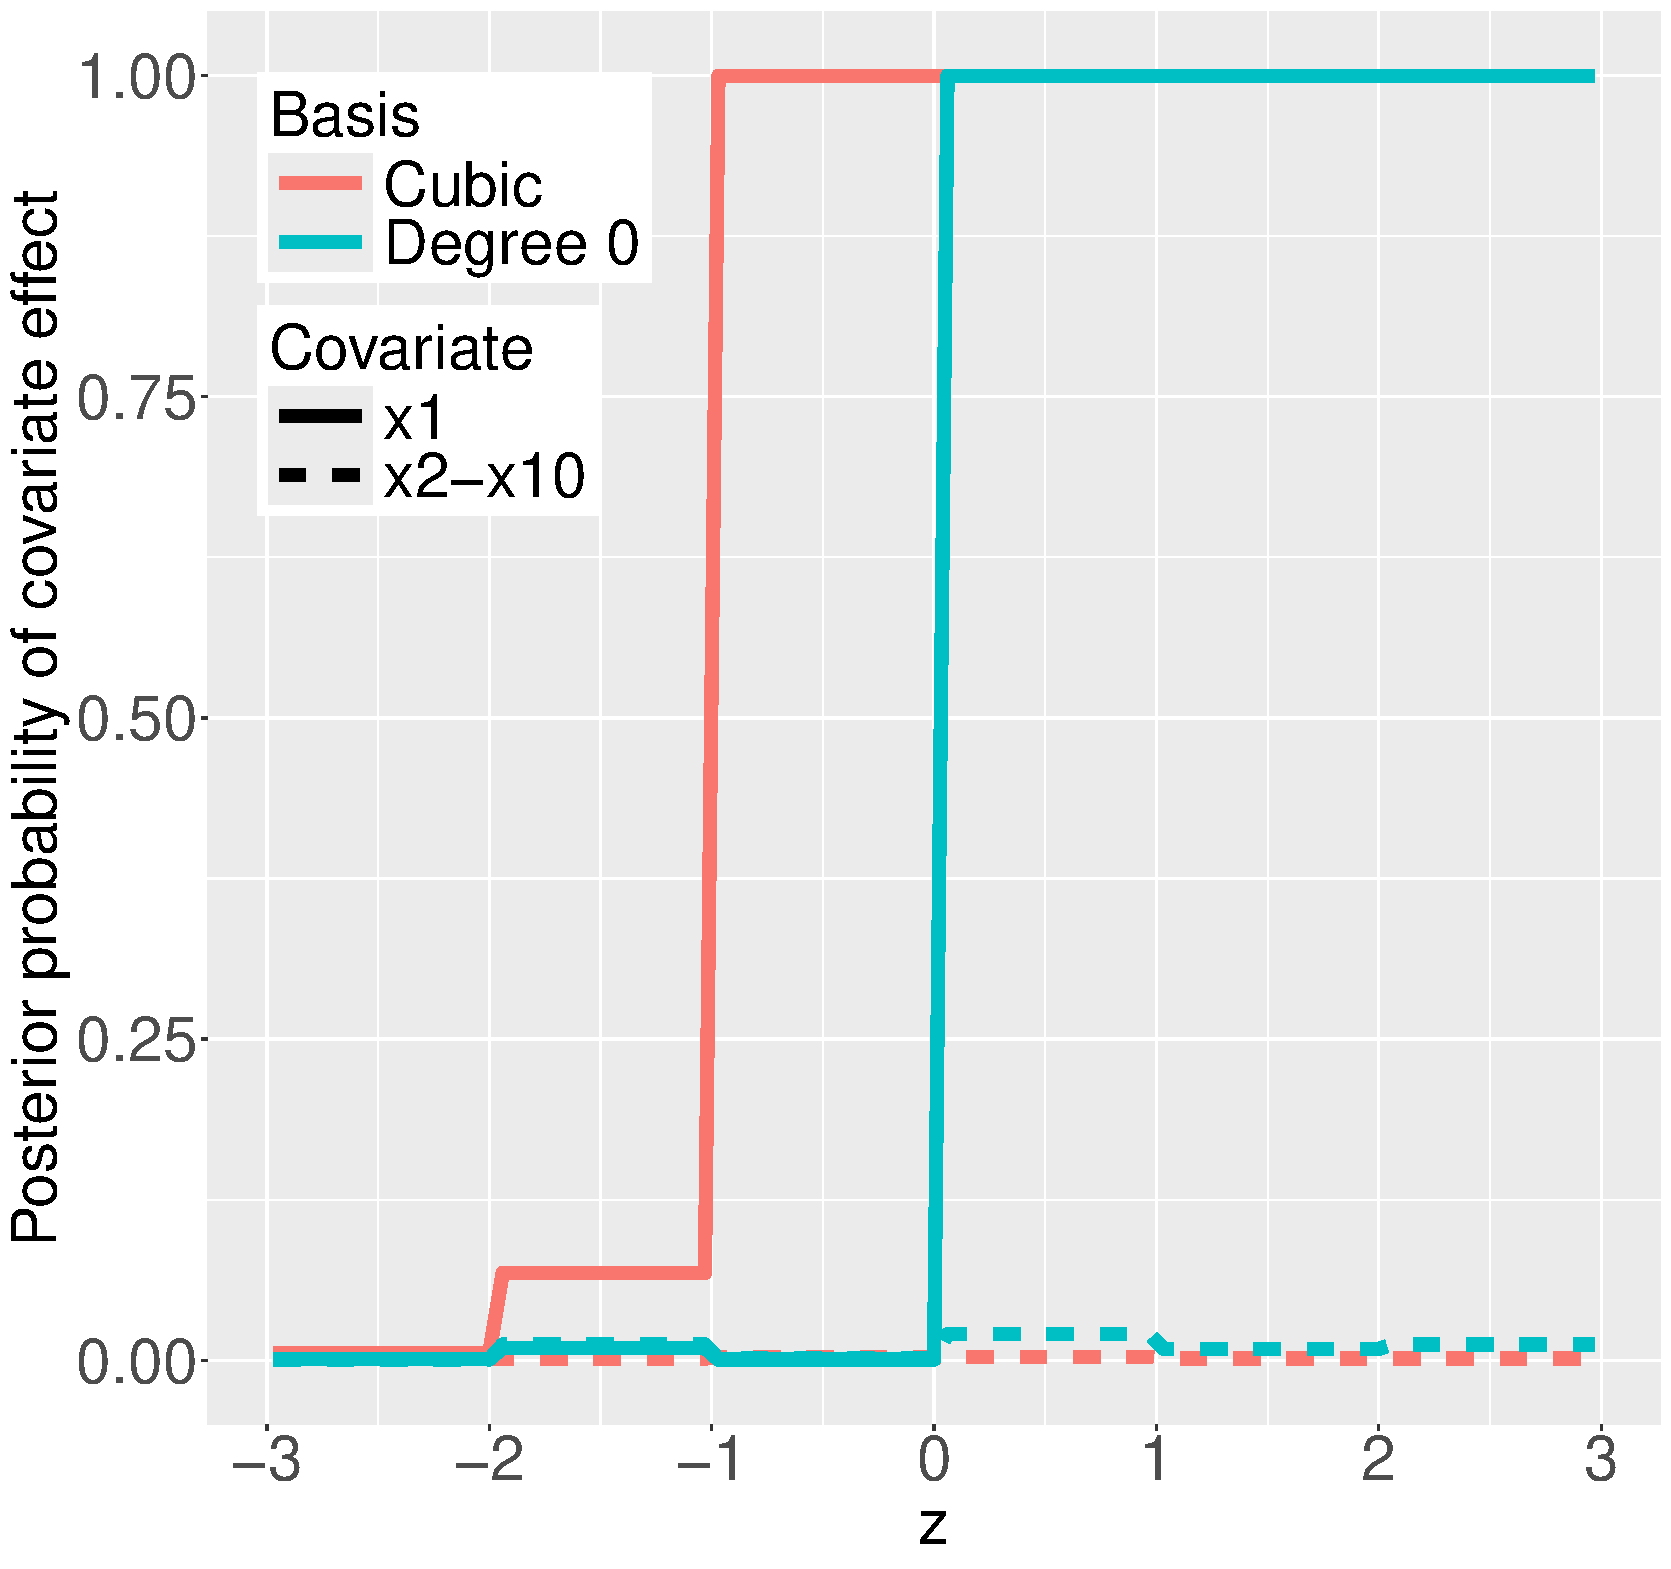
\includegraphics[width=0.5\textwidth,height=0.4\textwidth]{figs/simiid_unaligned_pp_n1000.pdf} \\
\end{tabular}
\end{center}
\caption{ Independent errors simulation with unaligned knots. 
Data-generating truth (top), and average
posterior probability for a local effect for $n=100$ (middle) and $n=1,000$ (bottom) }
\label{fig:simiid_unaligned}
\end{figure}




\subsection{Simulation with independent errors, non equi-spaced knots}
\label{ssec:simulation_iid_nonequispaced}


We illustrate our methodology in a setting where some of the resolutions place non equi-spaced knots for $\beta_1(z)$, the effect of a binary covariate.
The data-generating truth and the knots for the four considered resolution levels are depicted in Figure \ref{fig:simiid_nonequispaced}, top left panel.
The simulation settings are as in Section \ref{ssec:simulation_iid_misalign}, except that here we consider a single covariate for simplicity, and an increased range of sample sizes $n = \{100,1000,5000\}$.
In particular, note that the knots are misaligned with the true change point at $z=0.15$.
Resolutions 1 and 3 are equi-spaced and set a total of 7 and 11 knots, respectively.
Resolutions 2 and 4 place the same knots as resolution 1 and 3 (respectively) for $z<0$, and twice as many knots for $z>0$.

The right panel in Figure \ref{fig:simiid_nonequispaced} shows the average posterior probability for a local covariate effect for each sample size.
The results are analogous to those in Figure \ref{fig:simiid_unaligned} where only equi-spaced knots were considered.

The bottom panel in Figure \ref{fig:simiid_nonequispaced} show the average posterior probability assigned to the 4 resolutions.
As expected, for the smaller sample size $n=100$ the more parsimonious resolution 1 is favored. For $n=1000$, resolutions 2 and 3 receive more posterior probability. Intuitively, this occurs because the larger numbers of knots in these resolutions allow approximating $\beta_1(z)$ better, and the sample size is large enough to estimate the corresponding parameters accurately enough.
Similarly, for $n=5000$ it is resolutions 2 and 4 which receive the most posterior probability. This is appealing, since these resolutions place more knots at $z>0$ where the data-generating $\beta_1(z)$ varies, and less knots for $z<0$ where $\beta_1(z)=0$ is constant.


\begin{figure}
\begin{center}
\begin{tabular}{cccc}
\multicolumn{2}{c}{Data-generating truth}      & \multicolumn{2}{c}{$P(\beta_1(z) \neq 0 \mid y)$} \\
\multicolumn{2}{c}{and knots for 4 resolutions}& \multicolumn{2}{c}{}\\
\multicolumn{2}{c}{\includegraphics[width=0.5\textwidth]{figs/simiid_unaligned_nonequispaced.pdf}} &
\multicolumn{2}{c}{\includegraphics[width=0.5\textwidth]{figs/simiid_unaligned_nonequispaced_pp.pdf}} \\
& & & \\ %\hline
                             &  $n=100$ &  $n=1000$ &  $n=5000$ \\ %\hline
   Resolution 1  &  0.86    &  0.21     &  0.00     \\ 
   Resolution 2  &  0.01    &  0.30     &  0.55     \\ 
   Resolution 3  &  0.13    &  0.49     &  0.03     \\ 
   Resolution 4  &  0.00    &  0.00     &  0.42     \\  %\hline
\end{tabular}
\end{center}
\caption{ Independent errors simulation with non-equispaced knots.
Top left: data-generating truth and four resolutions. Resolutions 1 and 3 have the same number of knots for $z<0$ and $z>0$.
Resolutions 2 and 4 have twice as many knots for $z>0$.
Top right: average $P(\beta_1(z) \neq 0 \mid y)$ for $n=100$, $n=1,000$ and $n=5,000$.
Bottom: average posterior probability assigned to each resolution
 }
\label{fig:simiid_nonequispaced}
\end{figure}


%\begin{figure}
%\begin{center}
%\begin{tabular}{cc}
%Data-generating truth &  $P(\beta_1(z) \neq 0 \mid y)$ \\
%and knots for 4 resolutions & \\
%\includegraphics[width=0.5\textwidth]{../../figs/simiid_unaligned_nonequispaced.pdf} &
%\includegraphics[width=0.5\textwidth]{../../figs/simiid_unaligned_nonequispaced_pp.pdf} \\
%\end{tabular}
%\end{center}
%\caption{ Independent errors simulation with non-equispaced knots.
%Left: data-generating truth and four resolutions. Resolutions 1 and 3 have the same number of knots for $z<0$ and $z>0$.
%Resolutions 2 and 4 have twice as many knots for $z>0$.
%Right: average $P(\beta_1(z) \neq 0 \mid y)$ for $n=100$, $n=1,000$ and $n=5,000$ }
%\label{fig:simiid_nonequispaced}
%\end{figure}


%\begin{table}
%\begin{center}
%\begin{tabular}{lccc} %\hline
%                                              & n=100 & n=1000 & n=5000 \\ %\hline
%   7 knots, equi-spaced                       & 0.86 & 0.21 & 0.00 \\ 
%  11 knots (3 regions for z$<$0, 7 for z$>$0) & 0.01 & 0.30 & 0.55 \\ 
%  11 knots, equi-spaced                       & 0.13 & 0.49 & 0.03 \\ 
%  17 knots (5 regions for z$<$0, 11 for z$>$0) & 0.00 & 0.00 & 0.42 \\ 
%   %\hline
%\end{tabular}
%\end{center}
%\caption{Average posterior probability assigned to the 4 resolutions in Figure \ref{fig:simiid_nonequispaced}.}
%\label{tab:pp_localknots}
%\end{table}




\subsection{Simulation with independent errors, bivariate $z$}
\label{ssec:simulation_iid_bivar}


\begin{figure}
\begin{center}
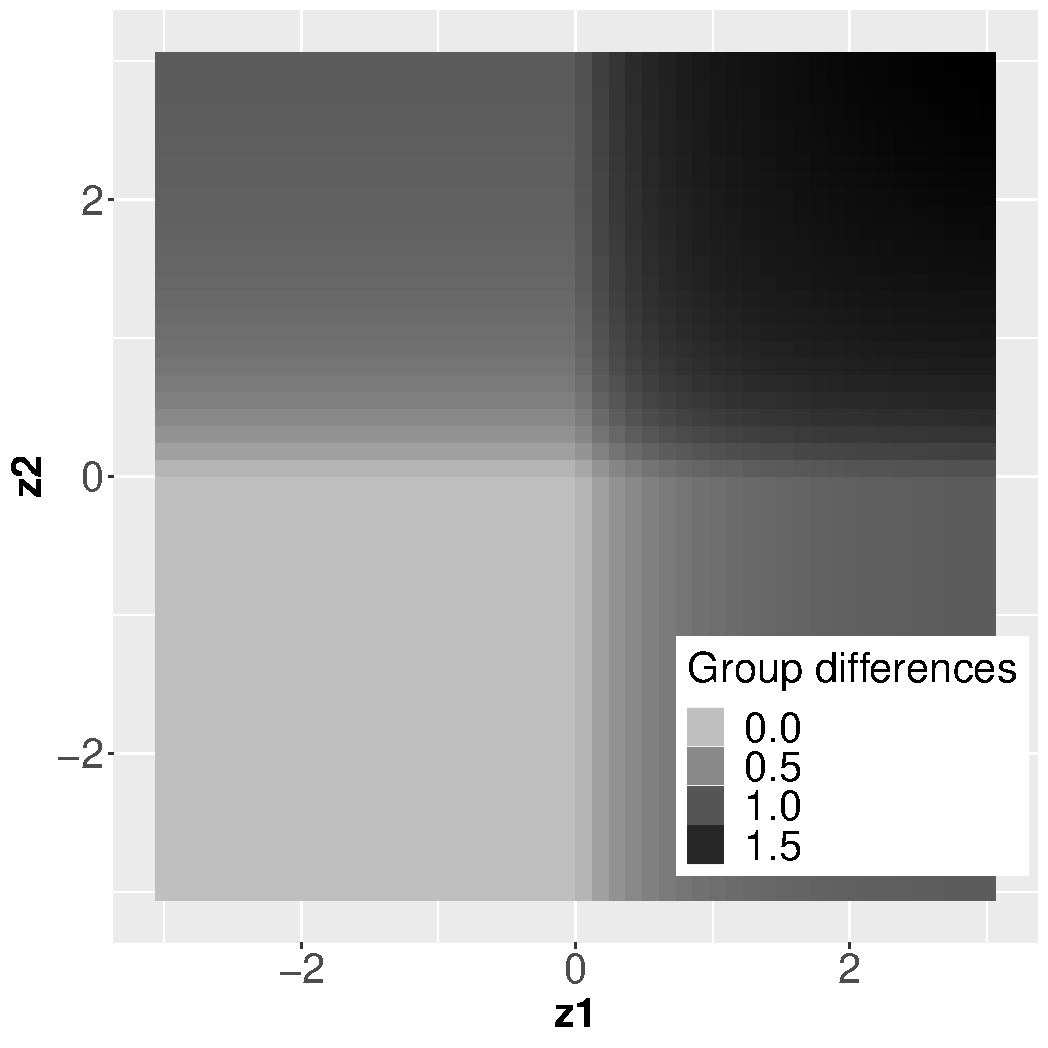
\includegraphics[width=0.6\textwidth]{figs/bspline_fit_cubic_bivar.pdf}
\end{center}
\caption{True group mean differences $E_F(y_i \mid x_{i1}=1, z_i) - E_F(y_i \mid x_{i1}=0, z_i)$ in bivariate $z$ simulation}
\label{fig:bspline_fit_cubic_bivar}
\end{figure}

\begin{figure}
\begin{center}
Covariate 1 \\
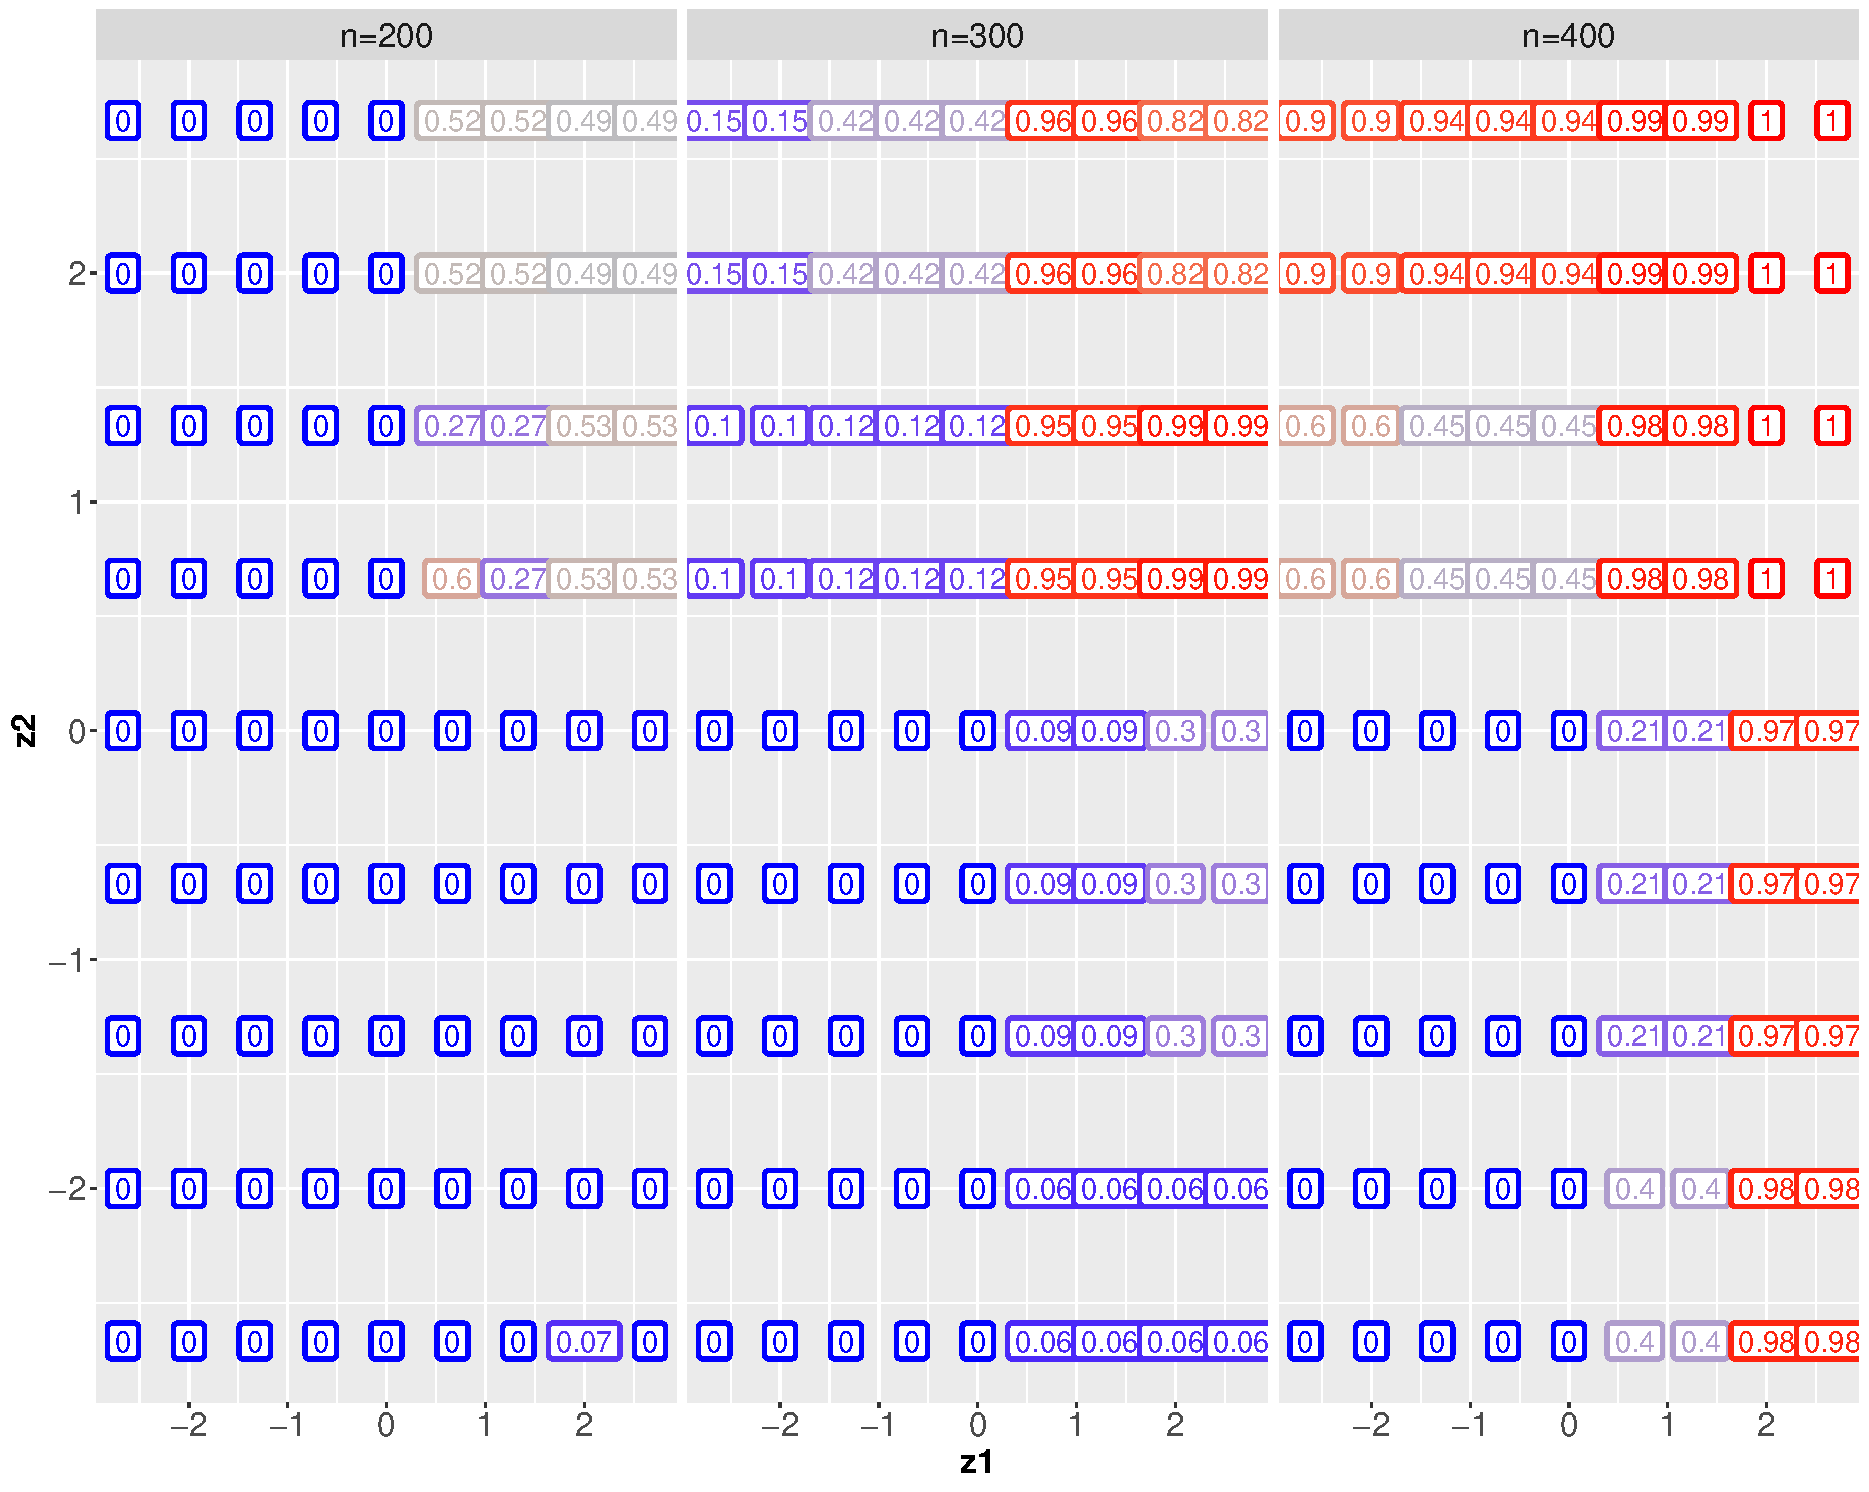
\includegraphics[width=1\textwidth, height=0.65\textwidth]{figs/simiid_pp_bivar_x1.pdf} \\
Covariates 2-10 \\
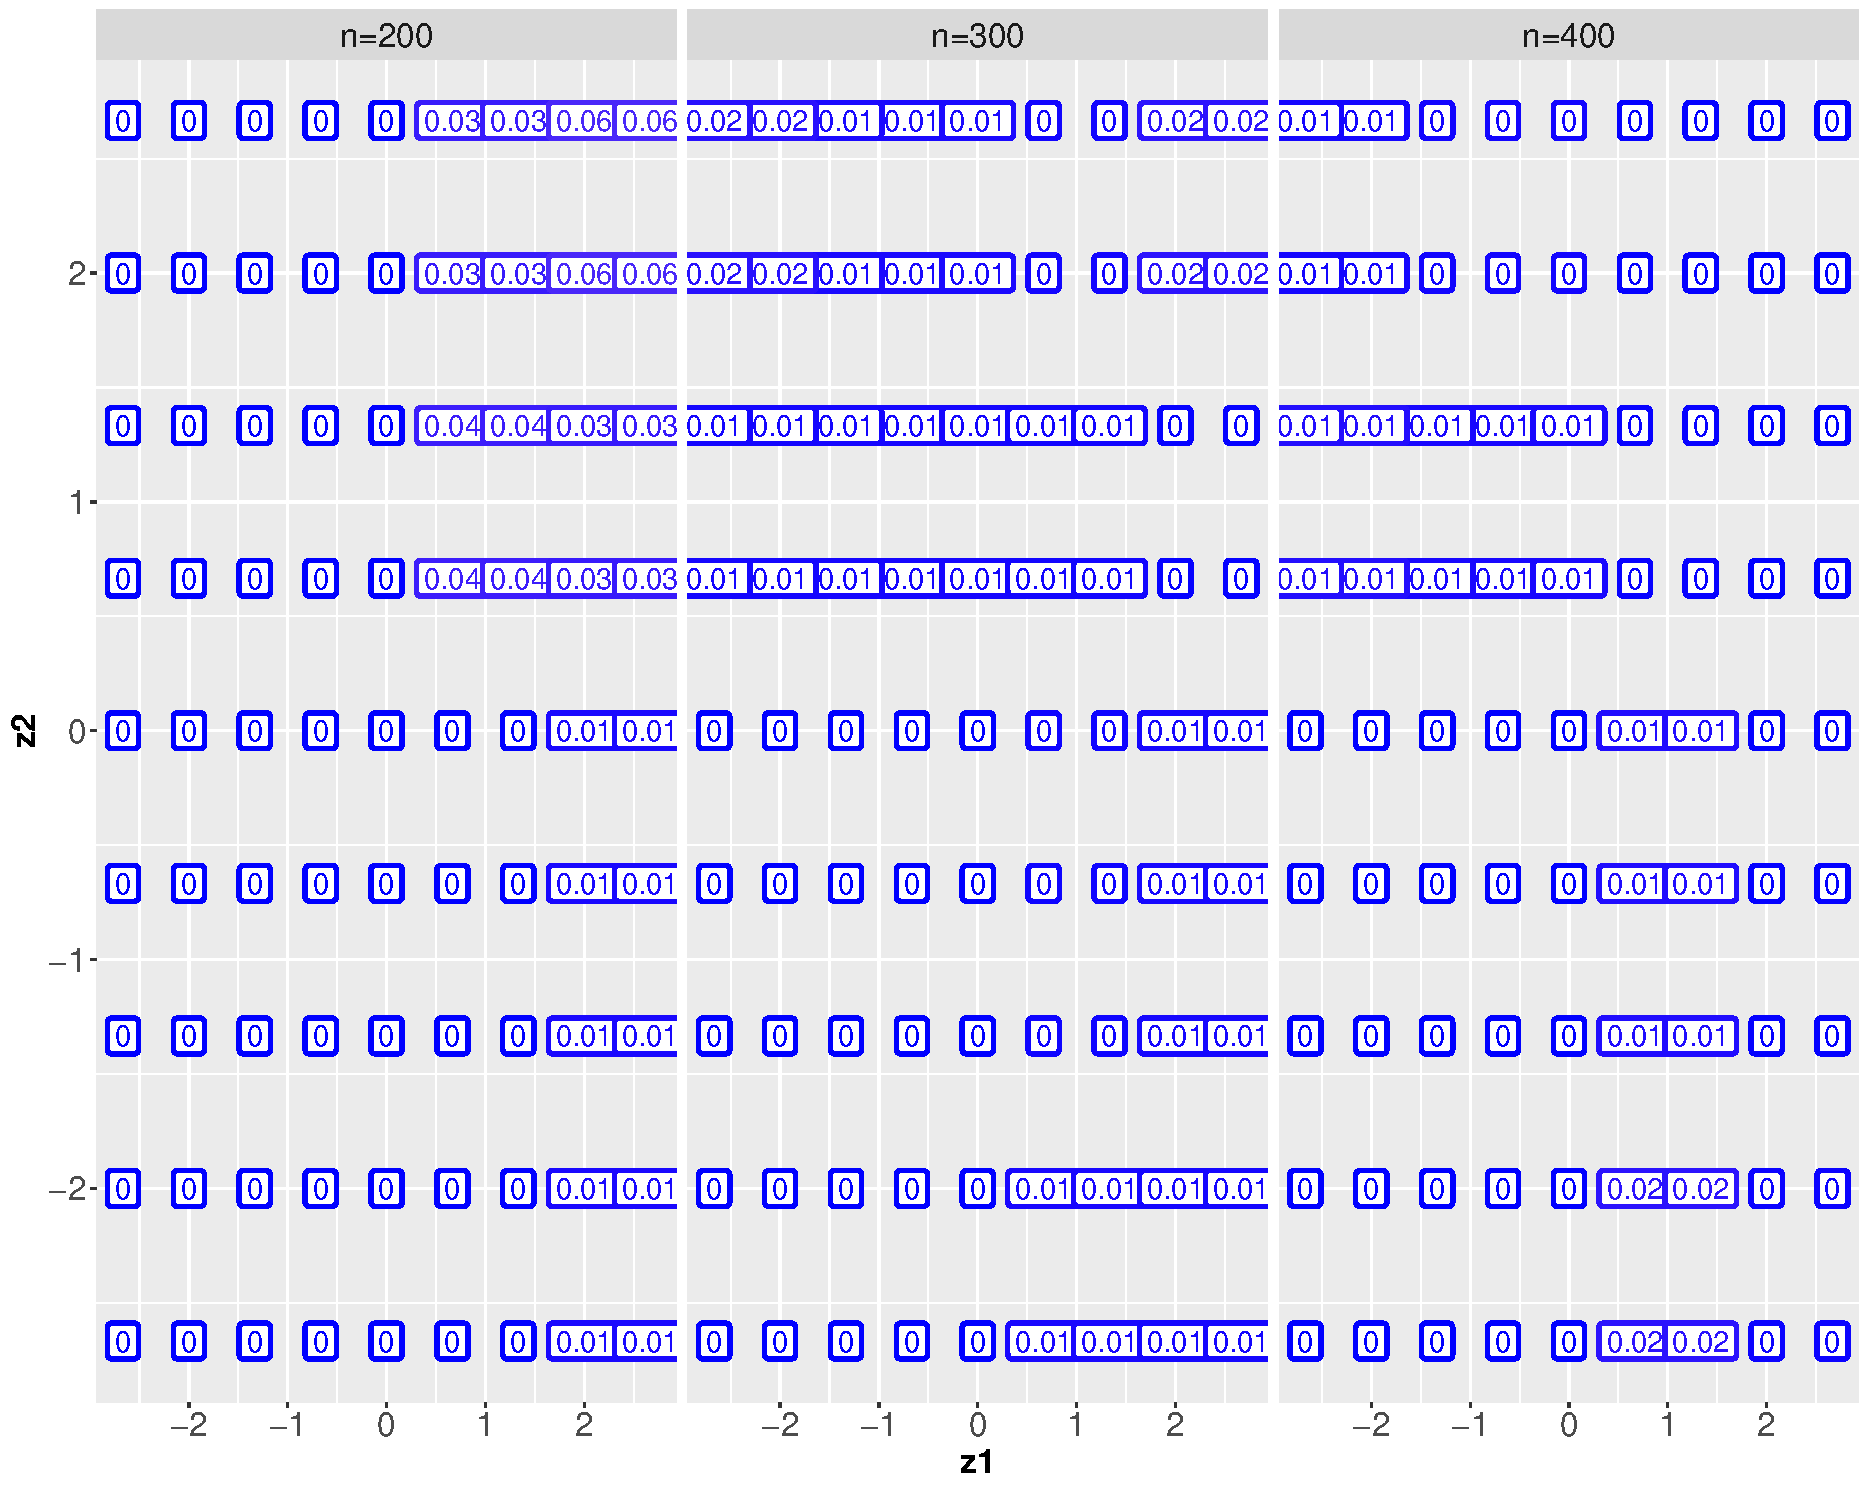
\includegraphics[width=1\textwidth, height=0.65\textwidth]{figs/simiid_pp_bivar_xother.pdf}
\end{center}
\caption{Simulation example with bivariate $z$ for $p=10$, $n=200, 300, 400$.
Posterior probabilities for a local effect of covariate 1 (truly active if $z_1>0$ or $z_2>0$) and inactive covariates 2-10}
\label{fig:simiid_bivar}
\end{figure}


Figure \ref{fig:simiid_bivar} shows a simulation study with bivariate $z$ that extends that presented in Section \ref{sec:simulation_iid}. The results are averaged across 50 independent simulations.
 We used a multi-resolution analysis that placed 5, 10 and 15 knots in each of the two dimensions. The average run time was 20 seconds using 1 core and 10 seconds using 3 cores on an Ubuntu Linux desktop, 13th Gen Intel core i7 processor, with 32Gb RAM. 
As in Section \ref{sec:simulation_iid} we consider $p=10$ covariates where $x_{i1}$ is binary and the remaining covariates $x_{i2},\ldots,x_{ip}$ are Gaussian, correlated with $x_{i1}$, and truly have no effect on the outcome. 
The true mean is set such that covariate $x_{i1}$ has an effect whenever $z_{i1}>0$ or $z_{i2}>0$.
Specifically, the true mean for group $x_{i1}=1$ is
\begin{align}
E_F(y_i \mid x_{i1}=0, z_i)= 
\sum_{j=1}^2 \mbox{I}(z_{ij} \leq 0) \cos(z_{ij}) + \mbox{I}(z_{ij} \leq 0)
\nonumber
\end{align}
In contrast, for group $x_{i1}=0$ it is
\begin{align}
E_F(y_i \mid x_{i1}=0, z_i)= 
\sum_{j=1}^2 \mbox{I}(z_{ij} \leq 0) \cos(z_{ij}) + \mbox{I}(z_{ij} \leq 0) \frac{1}{(z_{ij}^2+1)^2}.
\nonumber
\end{align}
That is, the setting is akin to that in the top panels of Figure \ref{fig:splinefit}, with bivariate $z$. 
Figure \ref{fig:bspline_fit_cubic_bivar} shows the group differences $E_F(y_i \mid x_{i1}=1, z_i) - E_F(y_i \mid x_{i1}=0, z_i)$.
We consider sample sizes $n \in \{200, 300, 400\}$, which suffice to illustrate the transition from a low- to a high-power setting.

The top panel in Figure \ref{fig:simiid_bivar} show that for $n=200$ the average marginal posterior probabilities for $x_{i1}$ are nearly zero, except for the region $(z_{i1}>0, z_{i2}>0)$, where the group differences are larger.
For $n=300$ and $n=400$ said posterior probabilities grow closer to 1 whenever there are truly group differences, but remain close to 0 for $(z_{i1}<0, z_{i2}<0)$ where there are no group differences.
The bottom panel shows how for covariates 2-10 the marginal probabilities remain close to zero for all $(z_{i1},z_{i2})$, indicating that the type I error probability is satisfactorily controlled.



\subsection{Functional data simulation}
\label{ssec:simulation_fda}

\begin{table}
\begin{center}
\begin{tabular}{ccccc} %\hline
\multicolumn{5}{c}{$M=50$ individuals}        \\ %\hline
& \multicolumn{2}{c}{Cut degree 0} & \multicolumn{2}{c}{VC-BART} \\
 Region         & Covariate 1 & Covariates 2-10 &  Covariate 1  &  Covariates 2-10  \\
$z \in $(-3,-2] & 0.06         & 0.080          &  0.60         &  0.58 \\ 
$z \in $(-2,-1] & 0.06         & 0.078          &  0.61         &  0.57 \\ 
$z \in $(-1,0]  & 0.056        & 0.072          &  0.61         &  0.58 \\ 
$z \in $(0,1]   & 0.73         & 0.084          &  0.82         &  0.56 \\ 
$z \in $(1,2]   & 0.873        & 0.070          &  0.97         &  0.56 \\ 
$z \in $(2,3]   & 1            & 0.057          &  0.98         &  0.54 \\ 
%\hline
\multicolumn{5}{c}{$M=100$ individuals} \\ %\hline
& \multicolumn{2}{c}{Cut degree 0} & \multicolumn{2}{c}{VC-BART} \\
 Region          & Covariate 1   & Covariates 2-10 &  Covariate 1 &  Covariates 2-10 \\
$z \in $ (-3,-2] & 0.05          & 0.036           &  0.64        &   0.58           \\
$z \in $ (-2,-1] & 0.045         & 0.038           &  0.72        &   0.52           \\ 
$z \in $ (-1,0]  & 0.0376        & 0.039           &  0.59        &   0.48           \\ 
$z \in $ (0,1]   & 0.99          & 0.036           &  0.89        &   0.52           \\ 
$z \in $ (1,2]   & 0.995         & 0.031           &  1           &   0.54           \\ 
$z \in $ (2,3]   & 1             & 0.027           &  1           &   0.51           \\ 
%\hline
\end{tabular}
\end{center}
\caption{Functional data simulation. Proportion of rejected null hypothesis for our 0-degree cut orthogonal basis,  and VC-BART.  For covariate 1 and $z>0$ this is the statistical power, otherwise it is the type I error}
\label{tab:simfda_10covar}
\end{table}


\begin{figure}
\begin{center}
\begin{tabular}{cc}
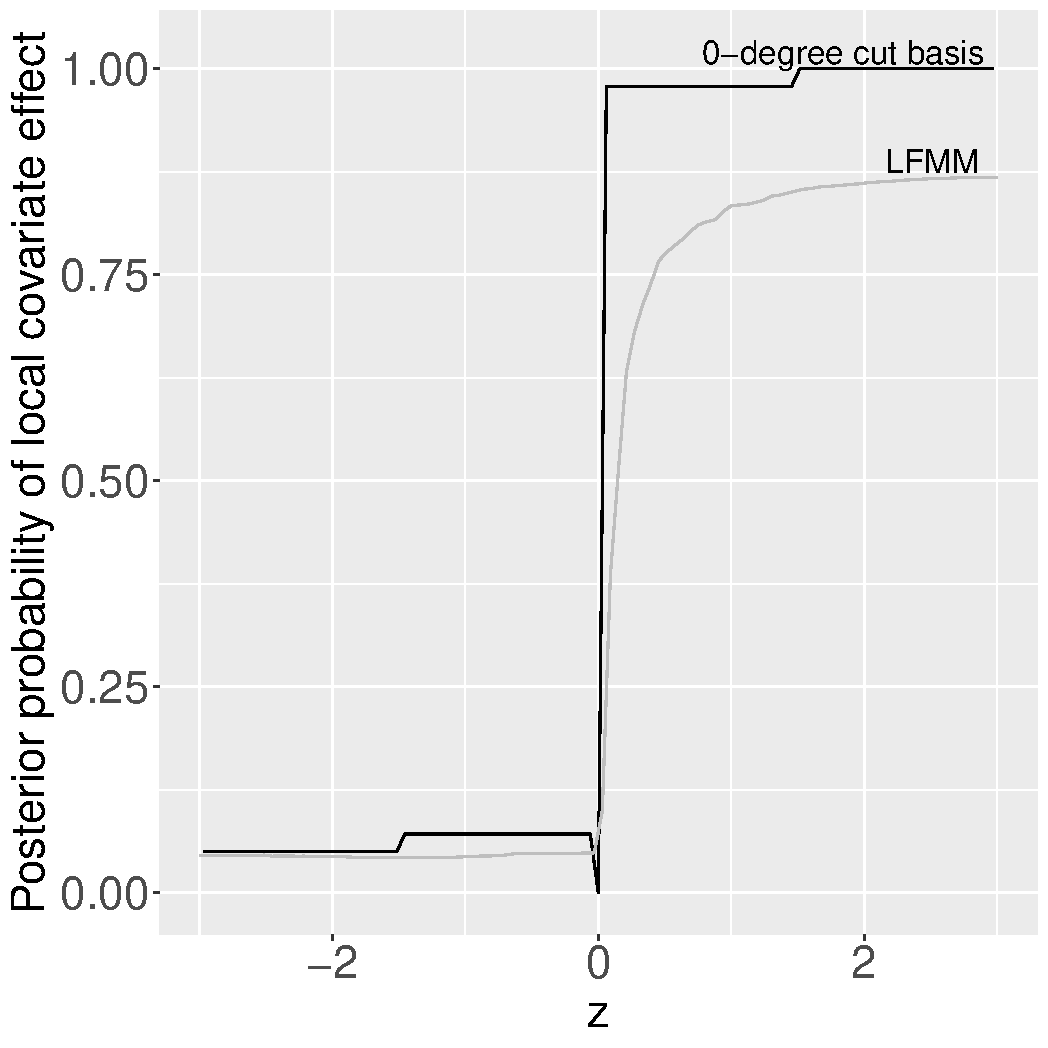
\includegraphics[width=0.48\textwidth]{figs/simfda_pp_single_nindiv50.pdf} &
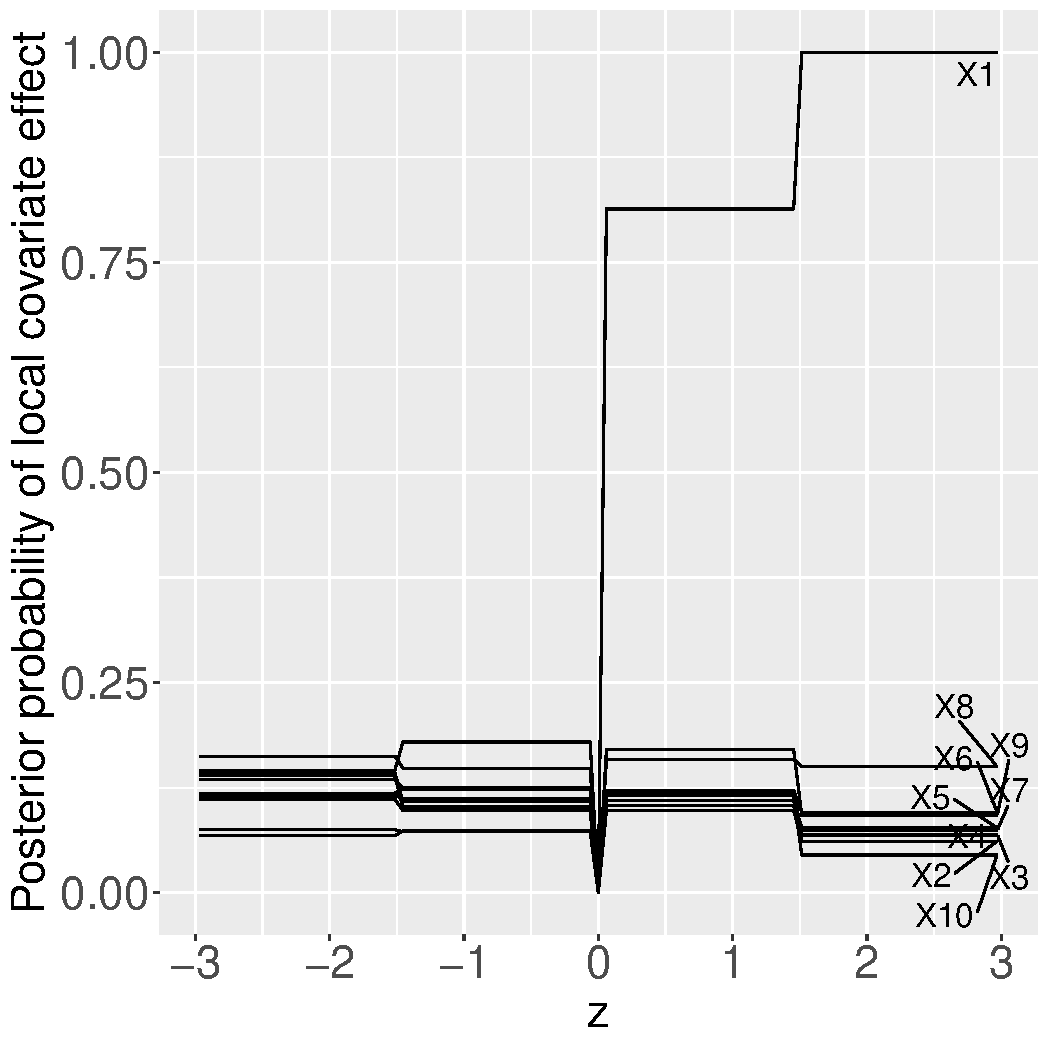
\includegraphics[width=0.48\textwidth]{figs/simfda_pp_nindiv50.pdf}
\end{tabular}
\end{center}
\caption{Functional data simulation. Posterior probability of a local covariate effect when using a single covariate (left) and 10 covariates (right)}
\label{fig:pp_simfda}
\end{figure}


Figure \ref{fig:pp_simfda} displays a comparison of the two Bayesian methods, our framework and tensor model (referred to by the acronym LFMM by its authors) proposed by \cite{paulon:2023}, in terms of the posterior probability assigned to the existence of a local covariate effect as a function of $z$ (averaged across 100 simulations).
The left panel is based on fitting the model where one only consider the truly active covariate 1, whereas the right panel also includes truly spurious covariates 2-10. Recall that covariate 1 truly has an effect only for $z>0$.


\subsection{Salary data}


\begin{figure}
\begin{center}
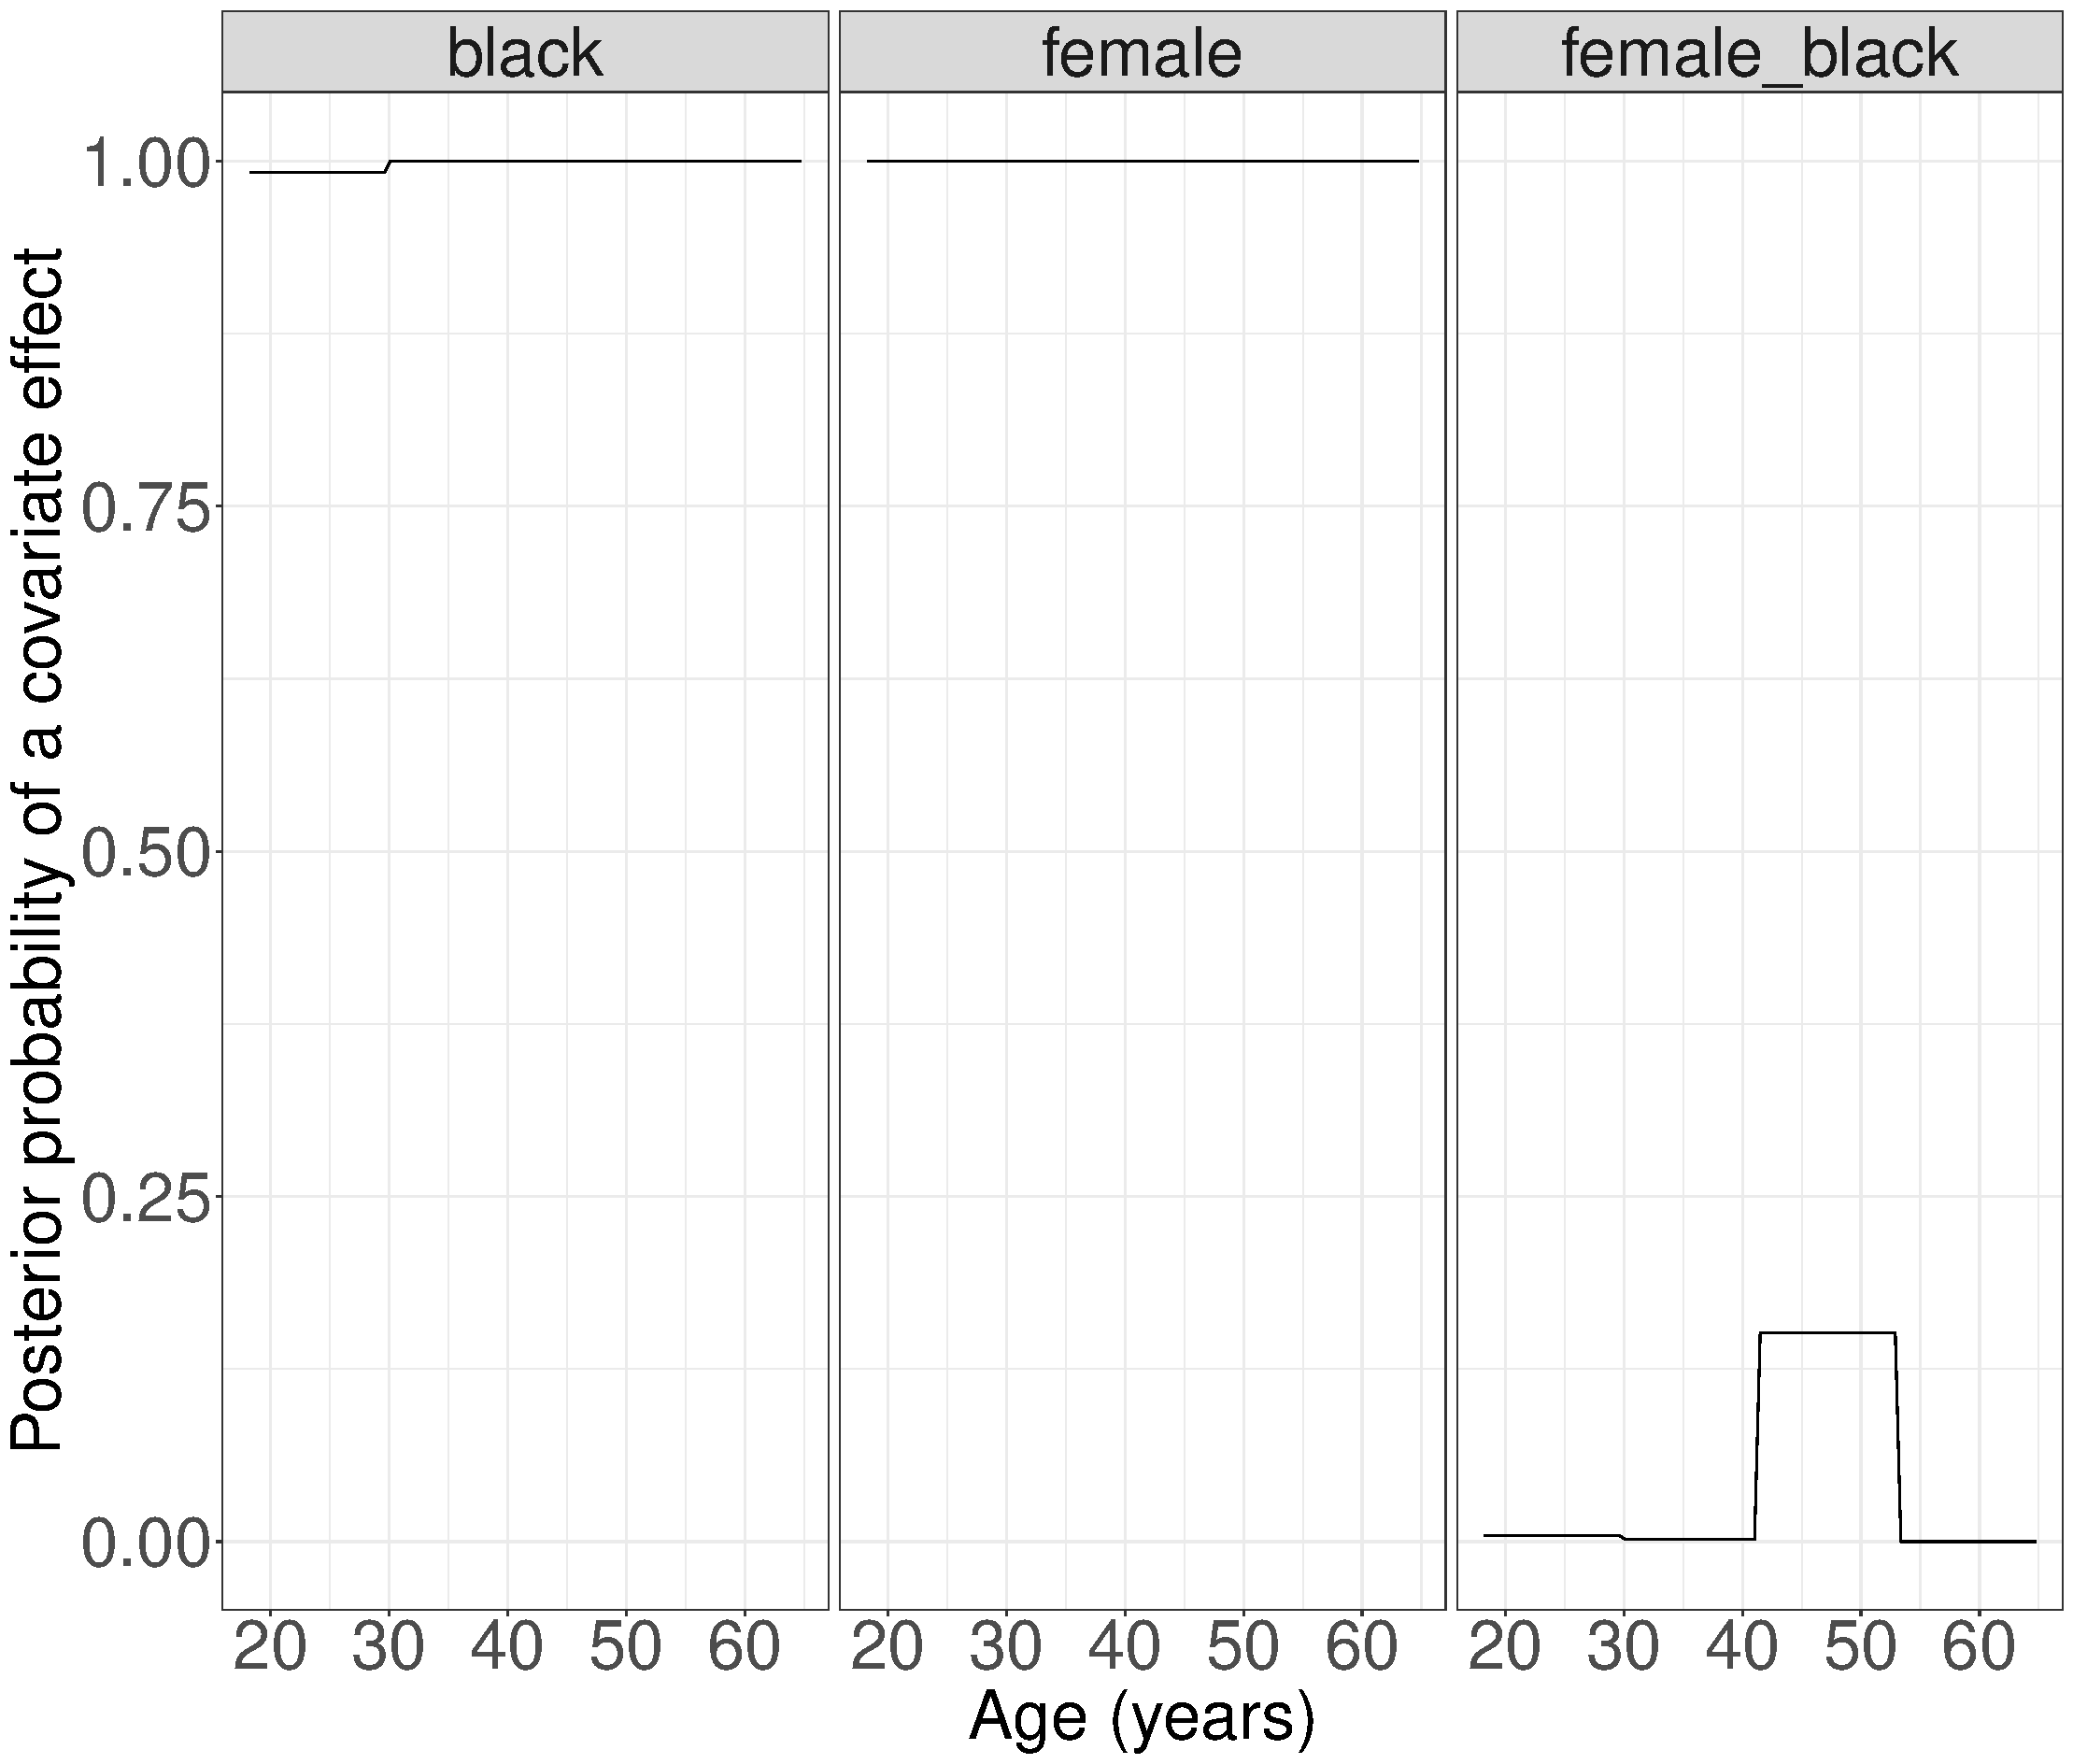
\includegraphics[width=0.7\textwidth]{figs/salary_pp_localtests_femaleblack.pdf}
\end{center}
\caption{Salary Data. Posterior probability of a salary gap associated with black race, sex and a black:sex interaction versus age, adjusted by occupation and worker class, and also including local effects for college, government, Hispanic race, and self-employment}
\label{fig:salary_female_race}
\end{figure}

\begin{figure}
\begin{center}
\begin{tabular}{cc}
\multicolumn{2}{c}{20 knots for baseline, 20 knots for local tests} \\
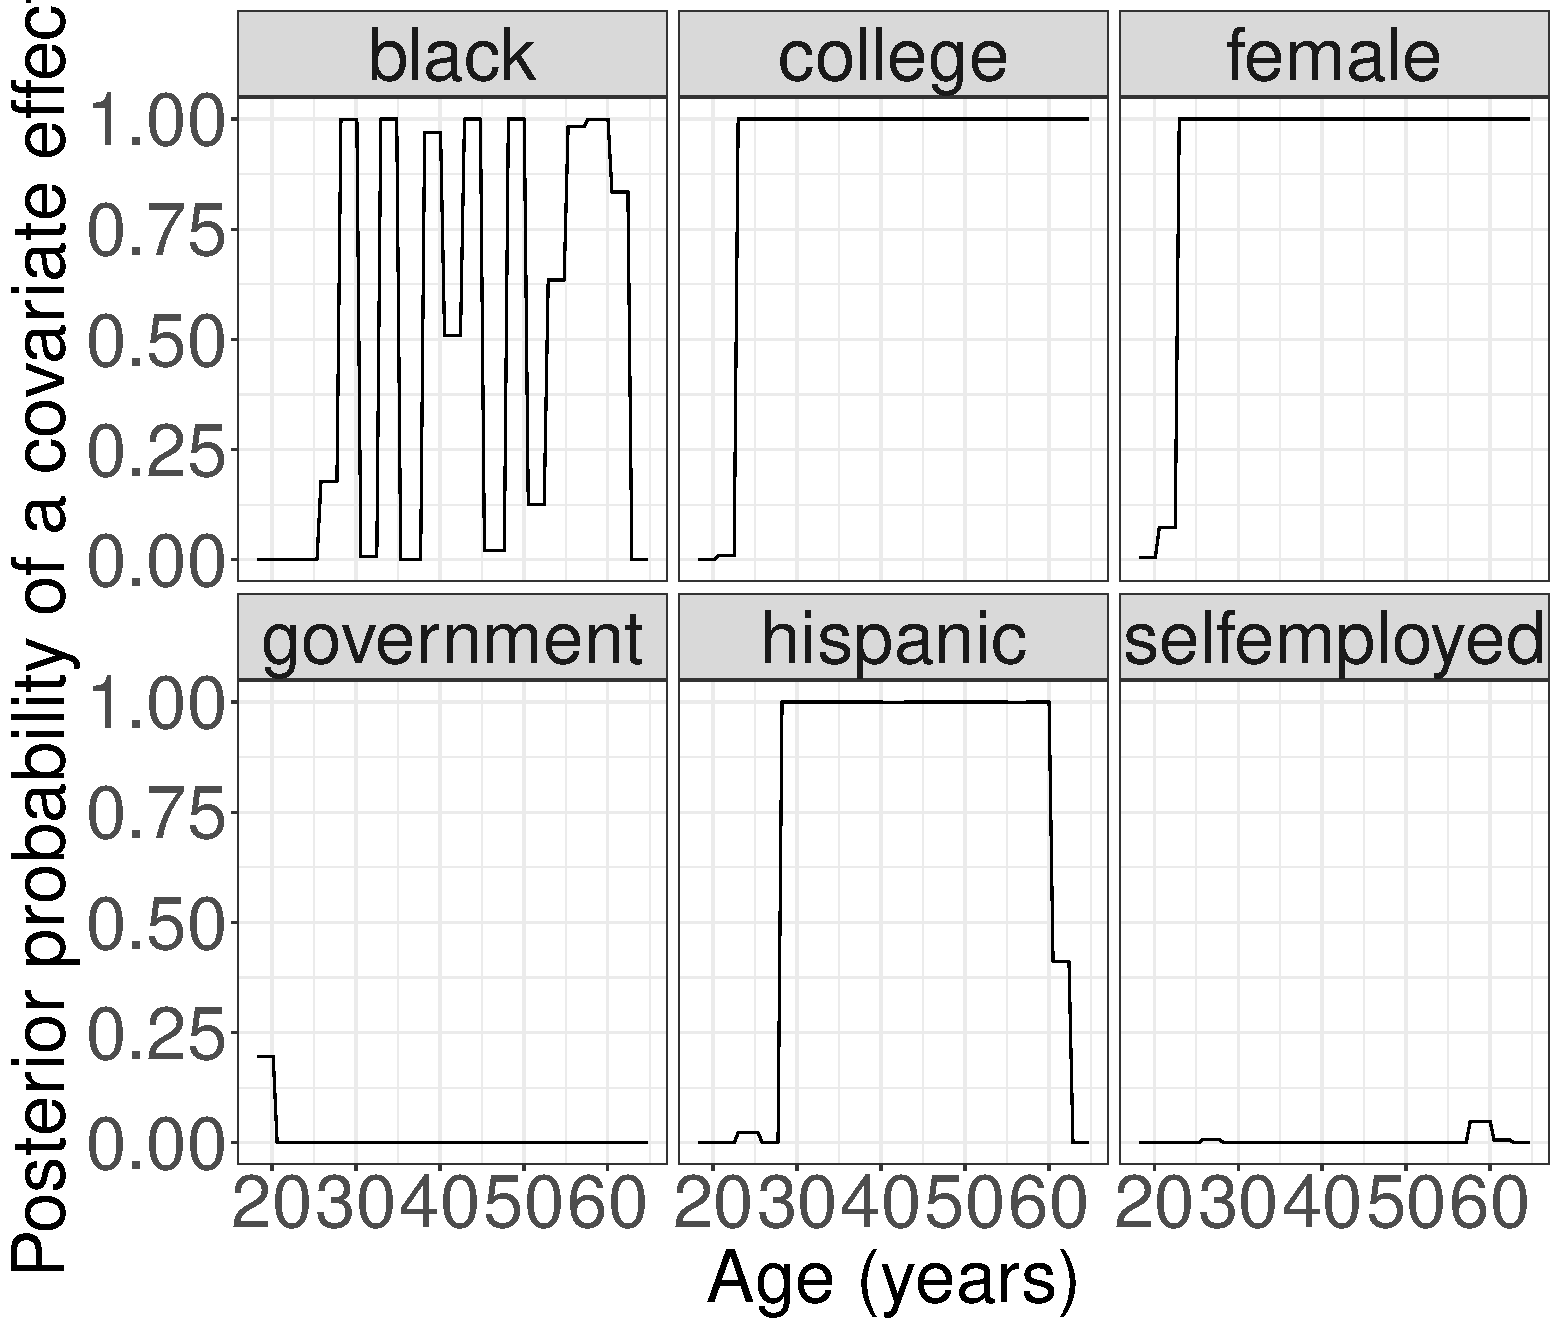
\includegraphics[width=0.5\textwidth]{figs/salary_pp_localtests_20knots.pdf} &
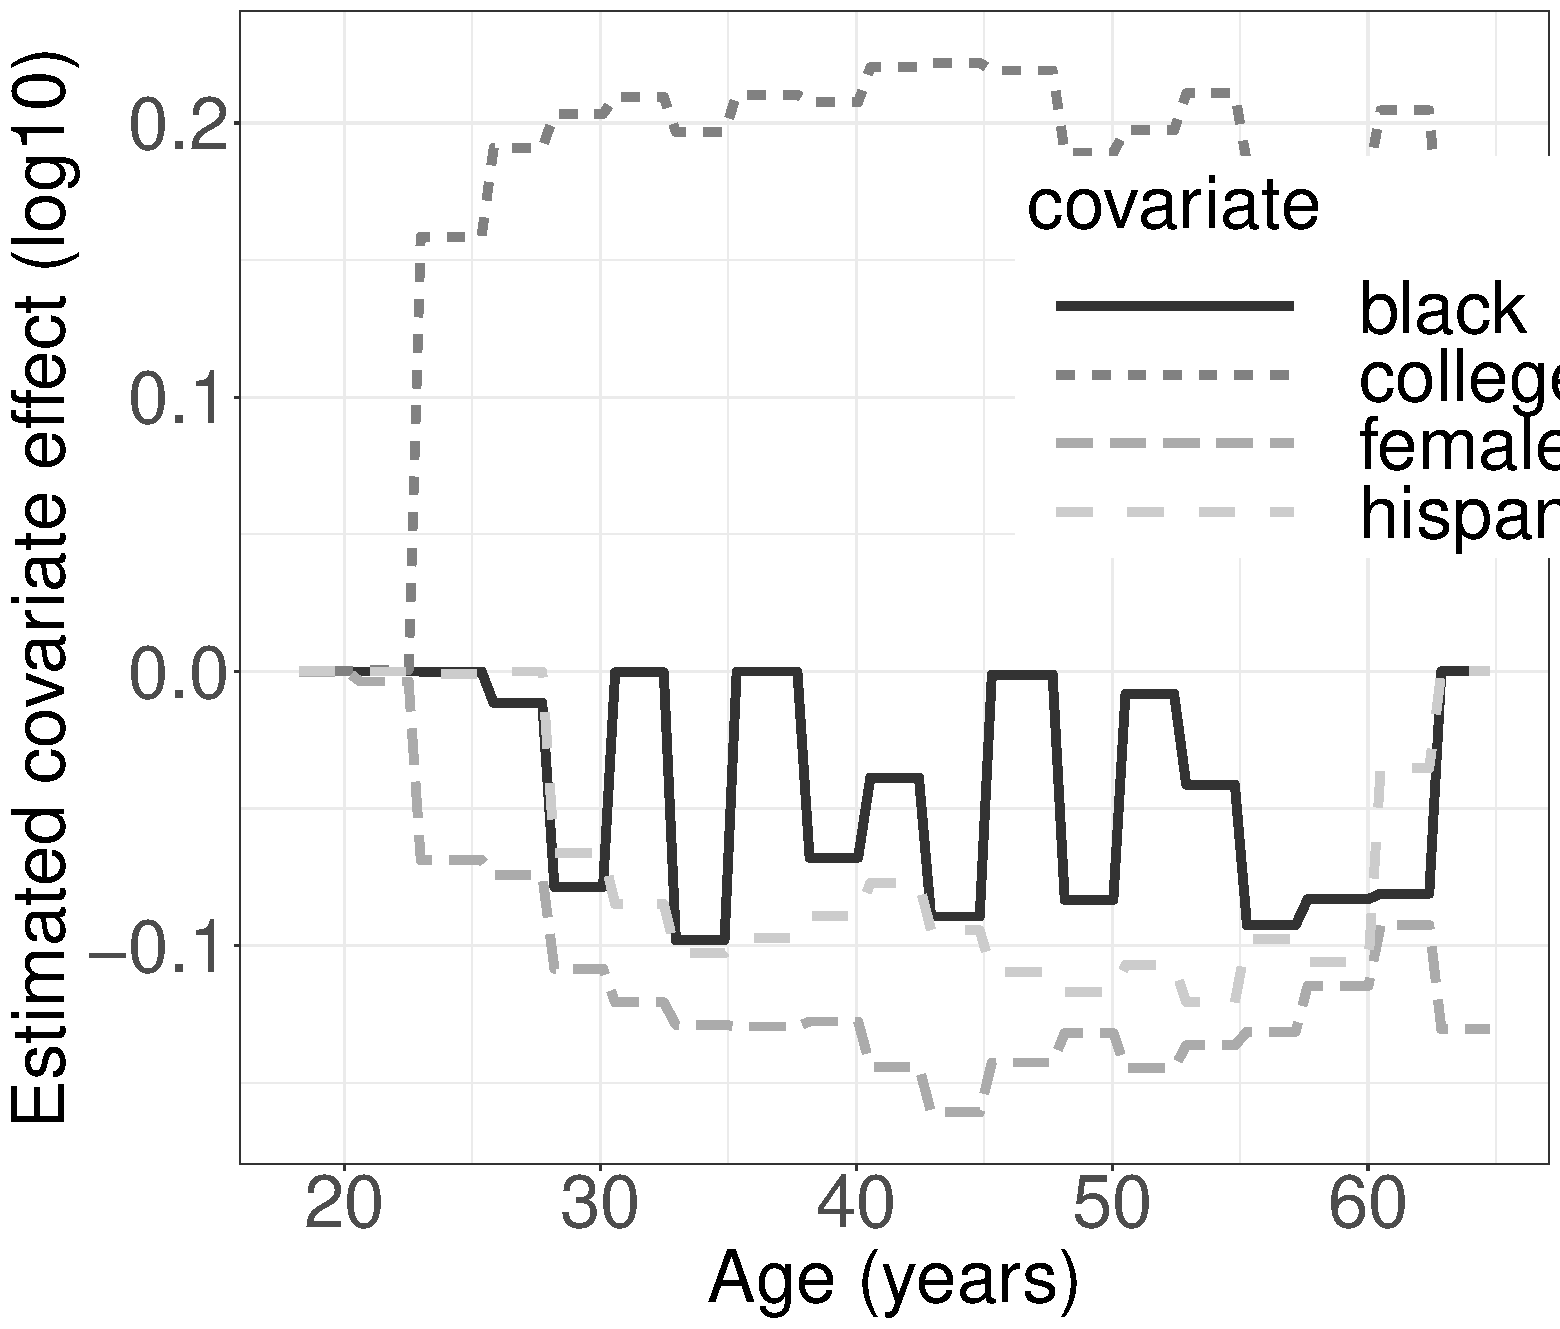
\includegraphics[width=0.5\textwidth]{figs/salary_estimated_effects_20knots.pdf} \\
%
\multicolumn{2}{c}{30 knots for baseline, 30 knots for local tests} \\
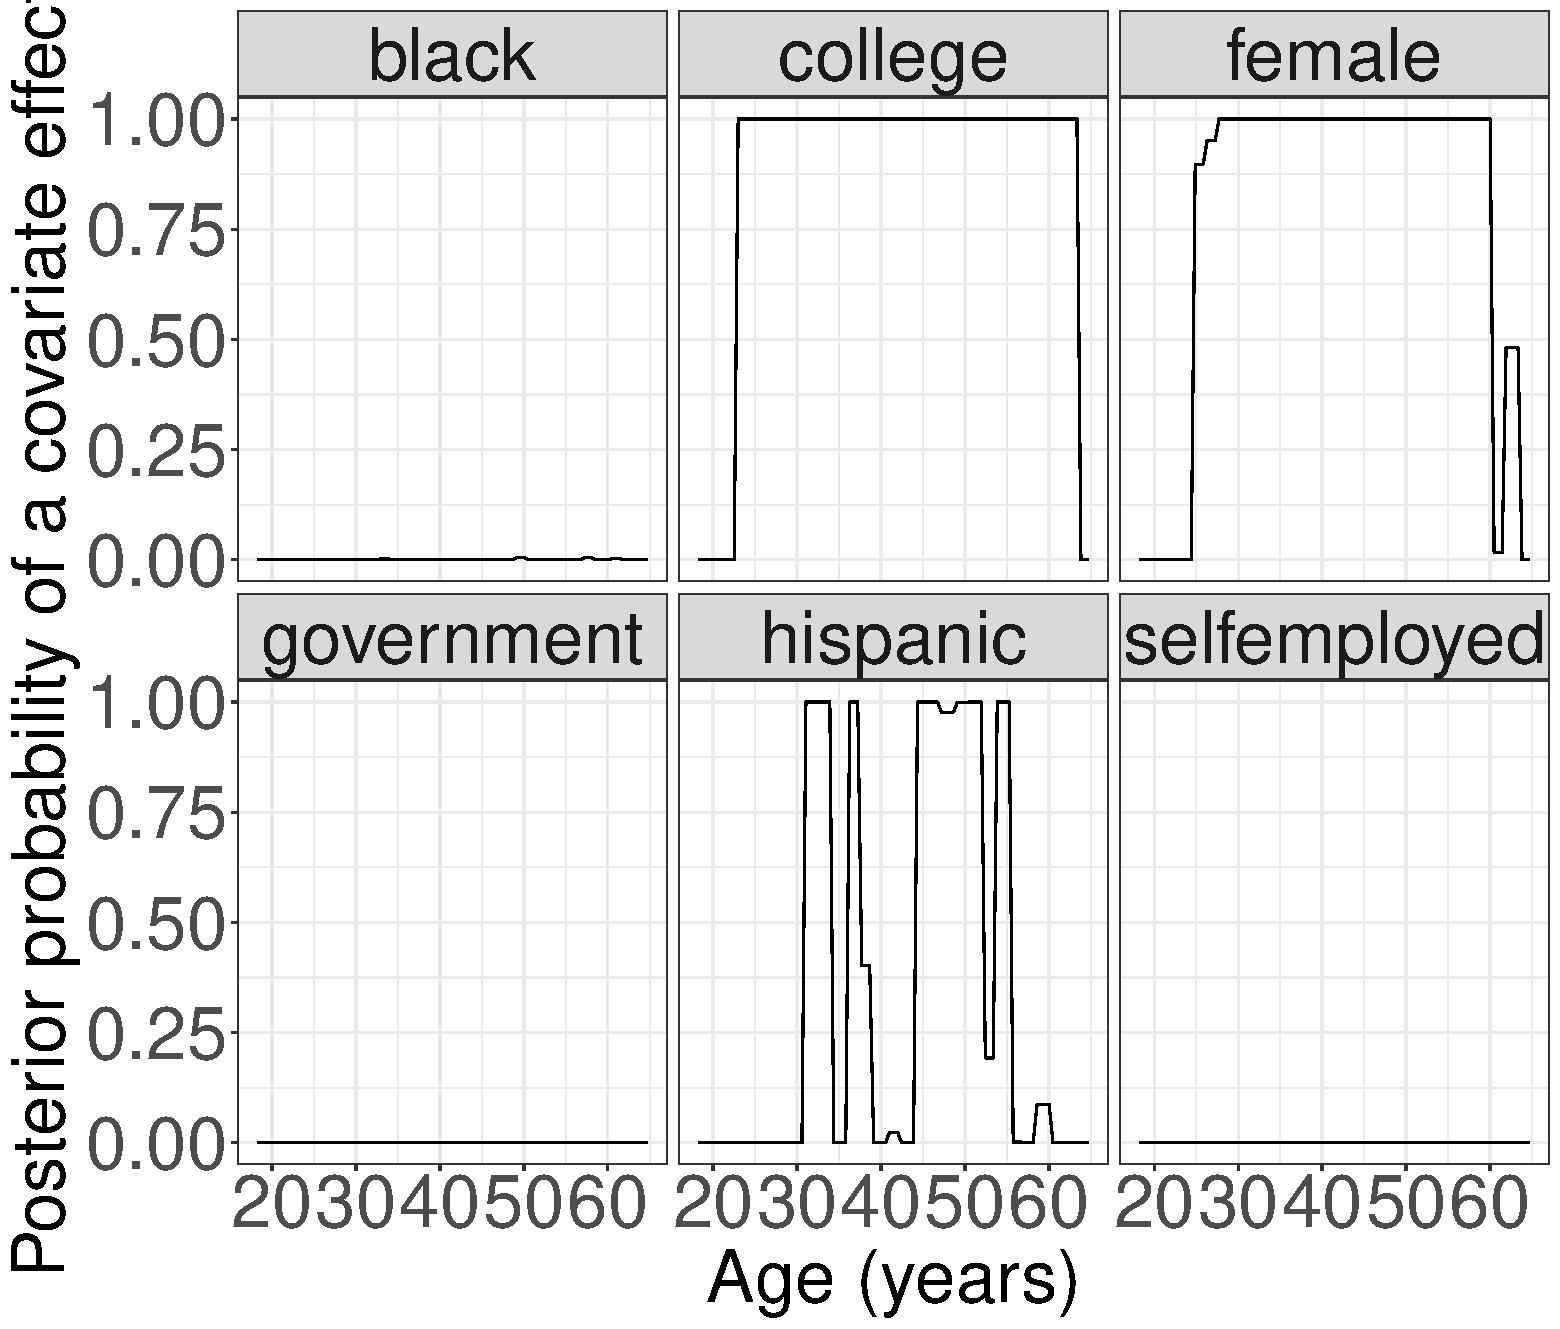
\includegraphics[width=0.5\textwidth]{figs/salary_pp_localtests_30knots.pdf} &
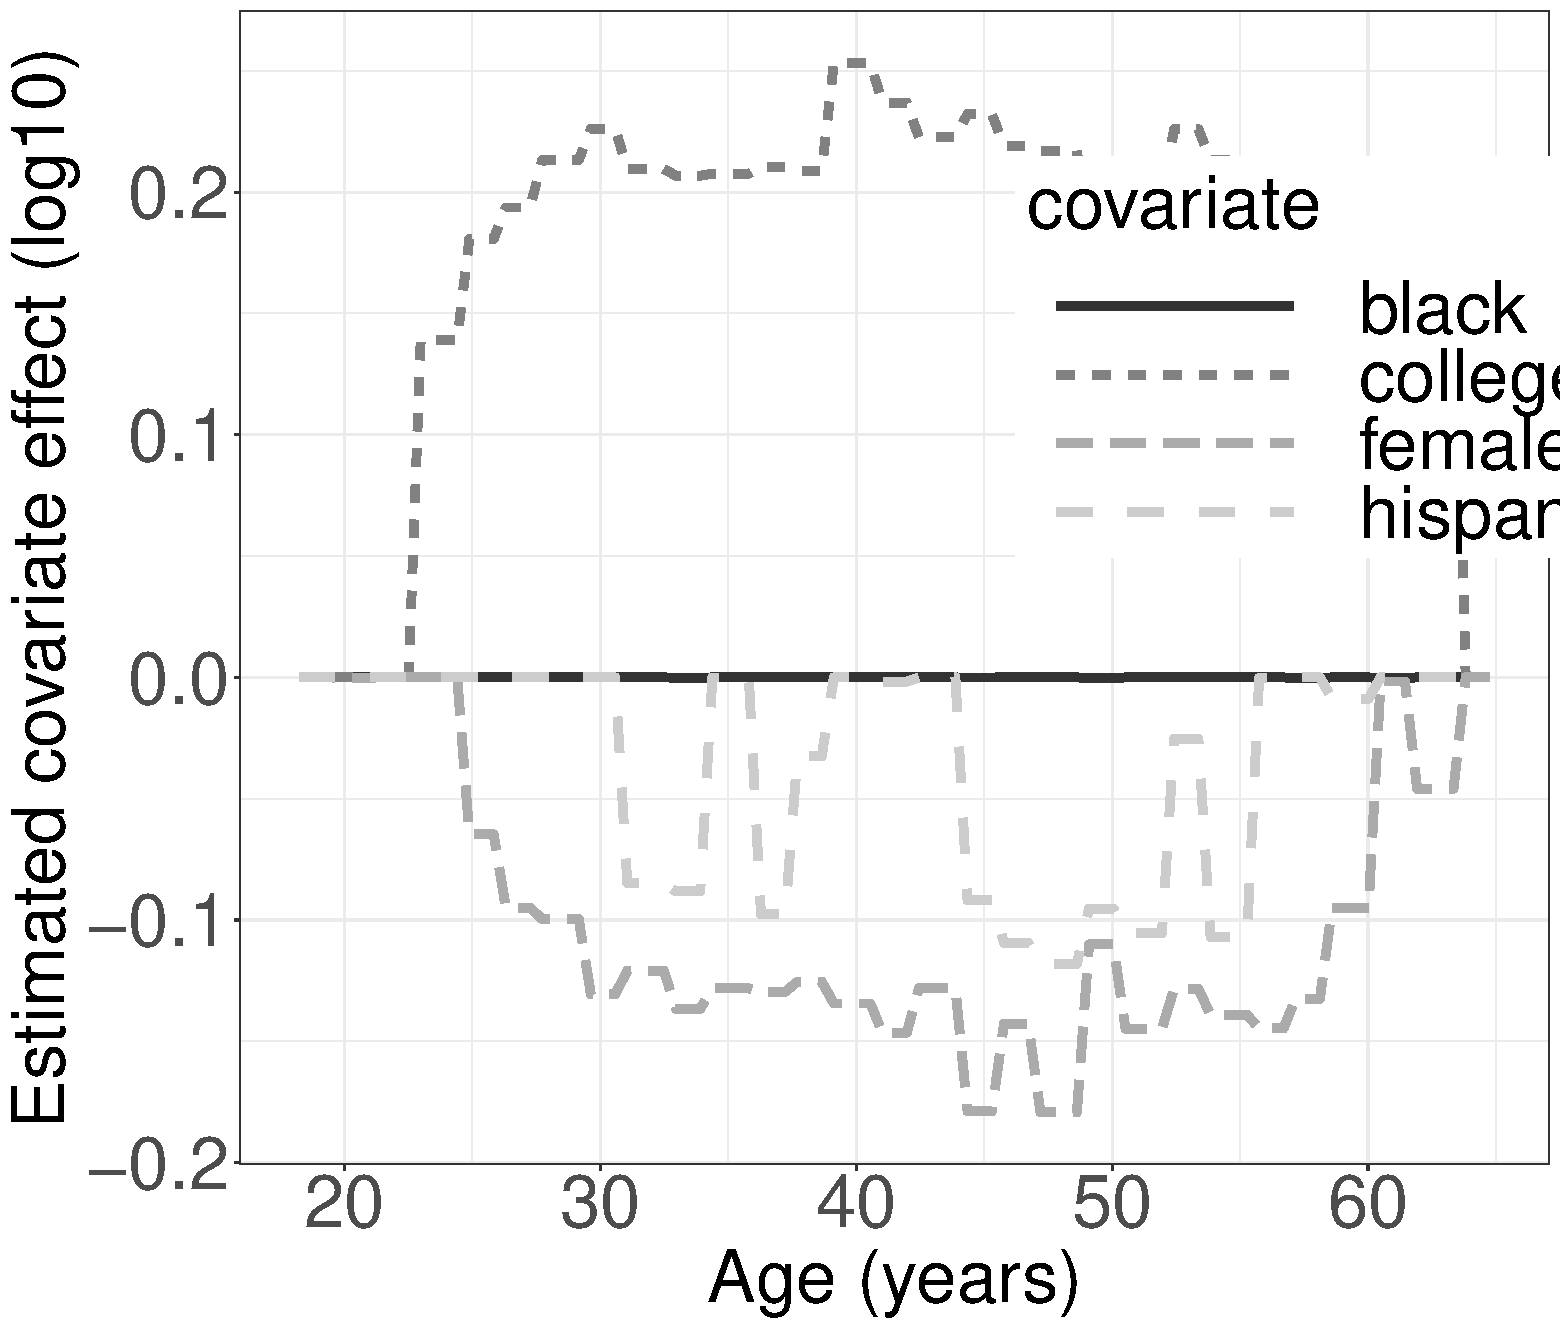
\includegraphics[width=0.5\textwidth]{figs/salary_estimated_effects_30knots.pdf}
\end{tabular}
\end{center}
\caption{Salary data results with fixed 20 (top) and 30 (bottom) fixed knots. 
Left: posterior probability of a salary gap associated with race, gender and college education versus age, adjusted by occupation and worker class. Right: corresponding estimated effect (log-10 scale)}
\label{fig:salary_suppl}
\end{figure}


The black race and female sex were found to be strongly associated to salary gap in our main analysis. To further explore this important source of potential salary discrimination, we repeated the analysis, now adding an interaction between black race and sex.
Figure \ref{fig:salary_female_race} shows that we obtained a small probability for the existence of said interaction, at all ages.


We also did additional analyses to assess the sensitivity of the results if one were to fix the number of knots, instead of using a multi-resolution analysis where one averages over resolutions.
Figure \ref{fig:salary_suppl} shows results for the salary data when fixing the number of knots to 20 (top panels) and 30 (bottom panels). The results suggest that, similar to what was observed in Figure \ref{fig:splinefit_suppl}, statistical power decreases when one adds more knots. This is apparent for covariates black and hispanic, which had the smaller estimated effects in our original analysis in Figure \ref{fig:salary} (where Bayesian model averaging was used to average over the uncertainty in the number of knots).
The results also suggest that there is no false positive inflation, covariates government and self-employed continue to show no local covariate effects at any age. Finally, covariates college and female are similar to our original analysis, in that they continue to be found to have a local effect on salary at almost all ages.



\subsection{Application to multi-electrode electrocorticography data}


\begin{figure}
	\begin{center}
		\begin{tabular}{cc}
		 	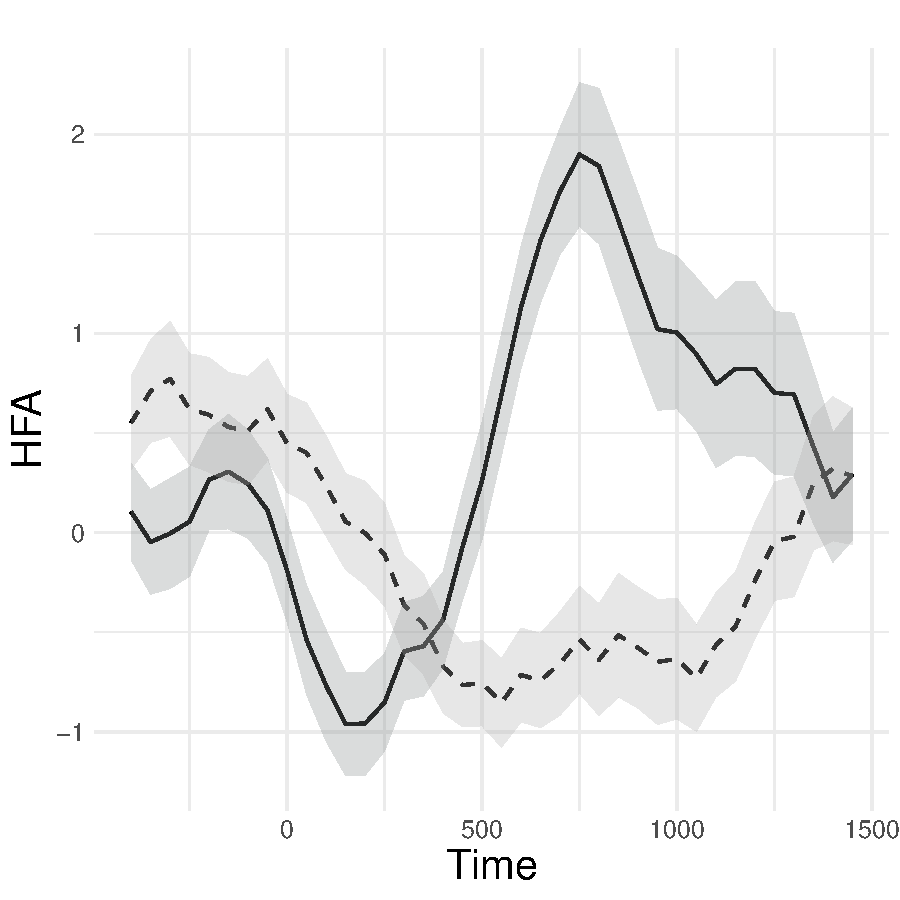
\includegraphics[width=0.45\textwidth]{figs/Ecog_trials1.pdf} &
			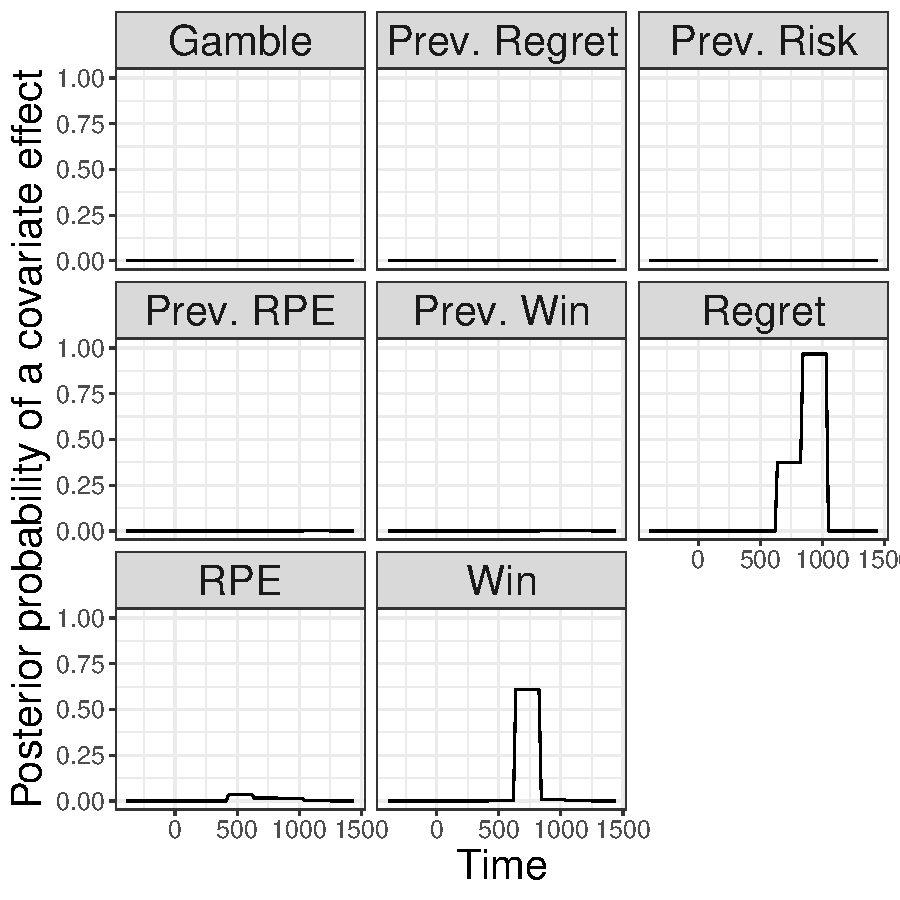
\includegraphics[width=0.5\textwidth]{figs/Ecog_pp_localtests_mr.pdf} 
		\end{tabular}
	\end{center}
	\caption{ECoG data. Left: mean high-frequency activity signal averaged across trials where the gamble was won (solid line) or lost  (dashed line), and point-wise 80\% confidence intervals. 
	Right: posterior probability of local covariate effects on brain activity}
	\label{fig:ECoG}
\end{figure}


\begin{figure}[htbp]
\begin{center}
\begin{tabular}{cc}
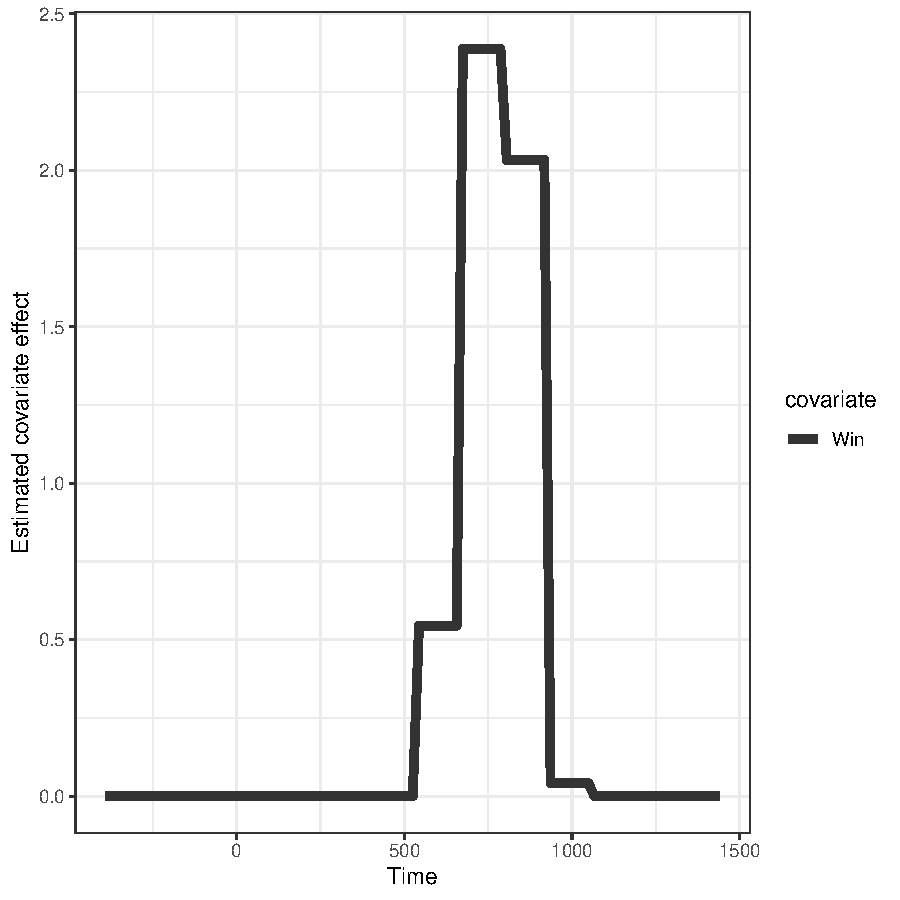
\includegraphics[width=0.45\textwidth]{figs/Ecog_estimate_fitwin.pdf} &
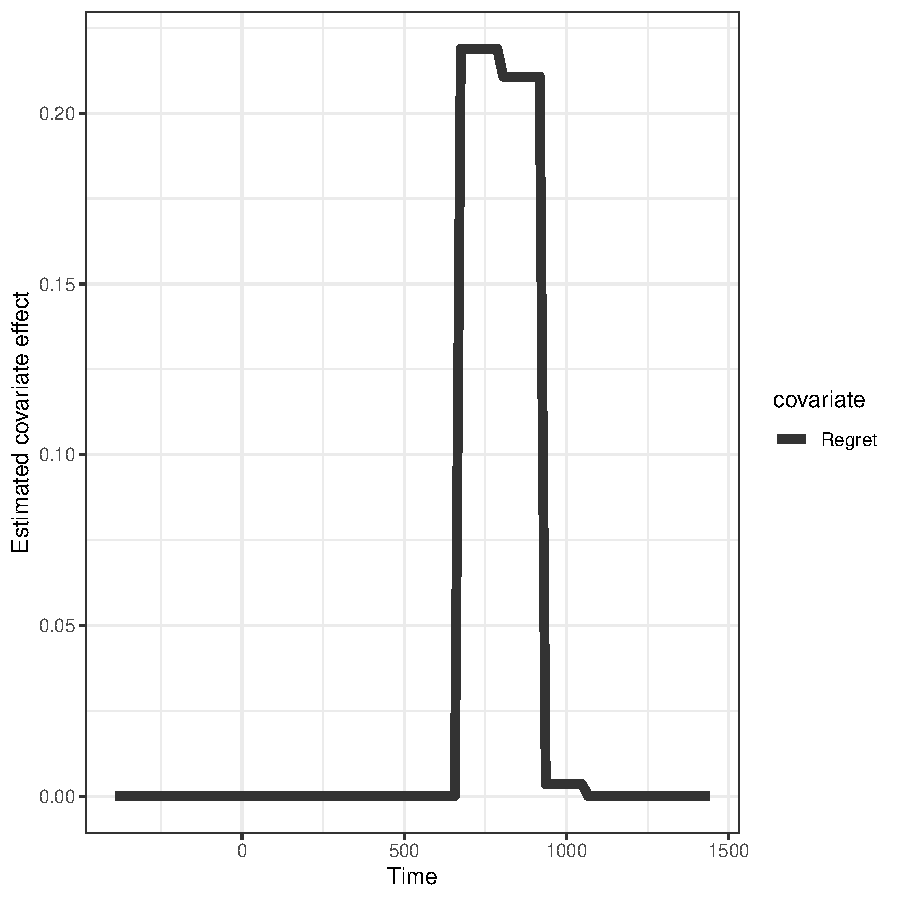
\includegraphics[width=0.45\textwidth]{figs/Ecog_estimate_fitregret.pdf} \\
Estimated effect of a Win/Loss over time &
Estimated effect of Regret over time \\
%
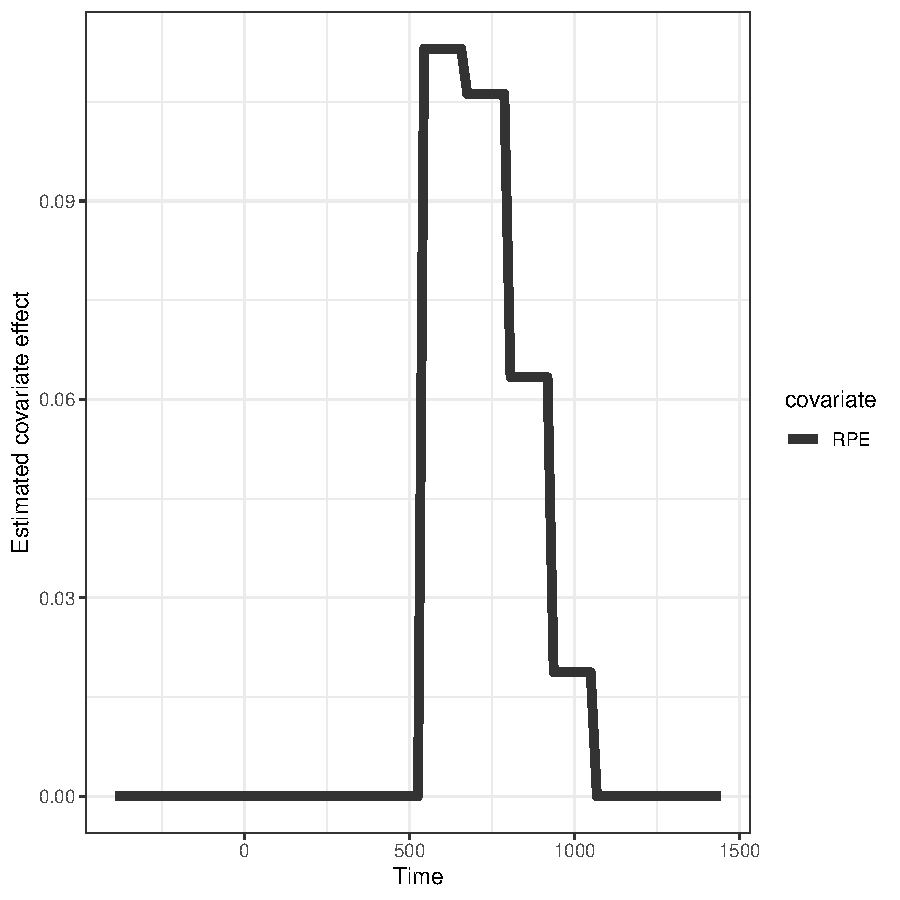
\includegraphics[width=0.45\textwidth]{figs/Ecog_estimate_fitrpe.pdf} &
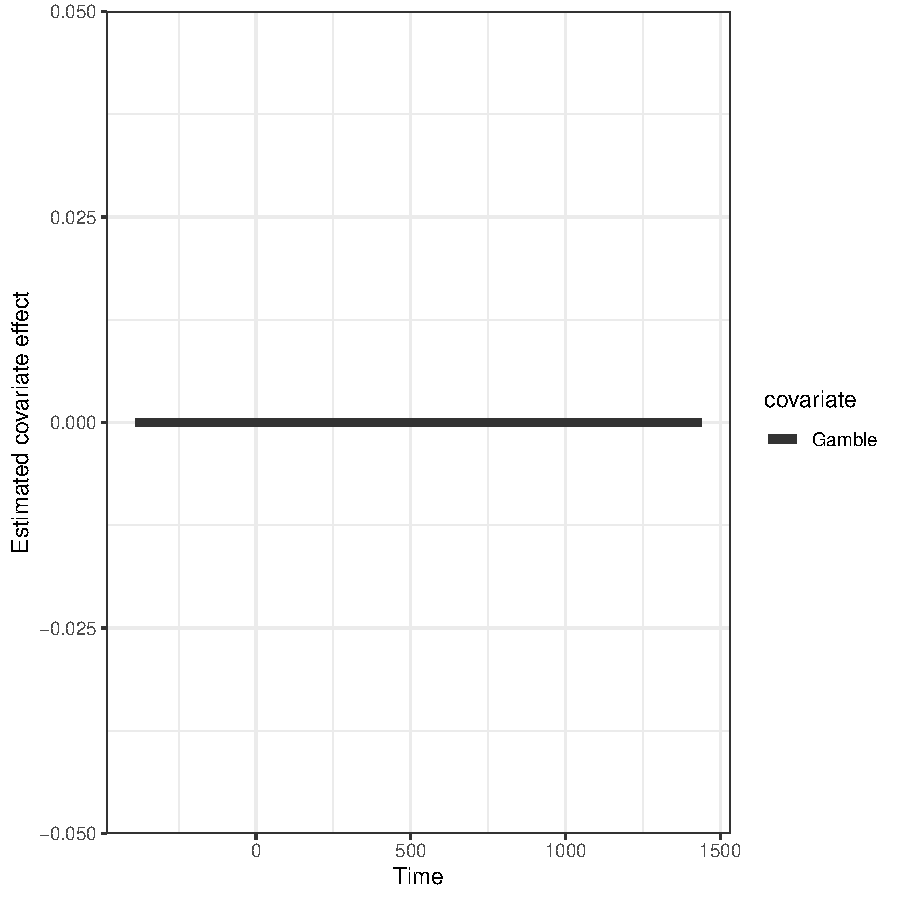
\includegraphics[width=0.45\textwidth]{figs/Ecog_estimate_fitgamble.pdf} \\
Estimated effect of the reward prediction error (RPE) over time &
Estimated effect of Gamble over time \\
\end{tabular}
\end{center}
\caption{Estimated time-varying effects of the three outcome-related covariates (Win, Regret, RPE) and the choice-related covariate Gamble in single-variate analyses for the application of Section \ref{ssec:saez_data}. Only Win and Regret show high posterior probabilities of having an effect on brain activity in the time intervals}
\label{fig:EcoG_effect_singles}
\end{figure}

\begin{figure}
	\begin{center}
		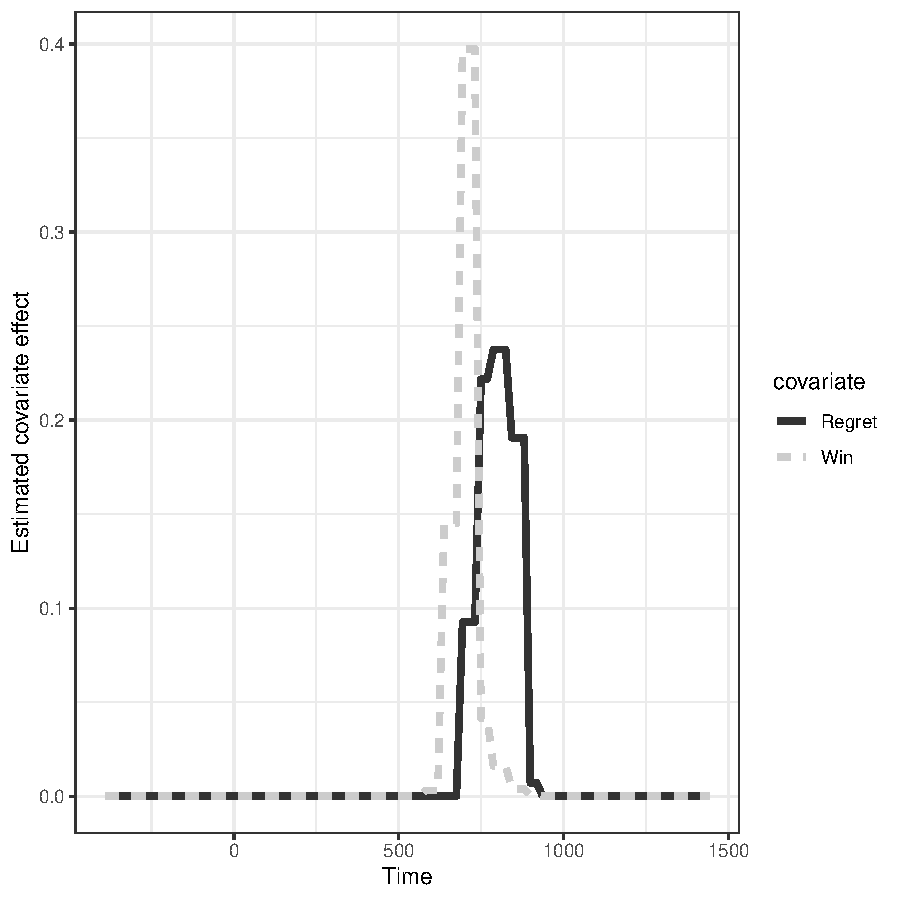
\includegraphics[width=0.7\textwidth]{figs//Ecog_estimate_fitmulti_mr.pdf}
	\end{center}
	\caption{Estimated time-varying effects of two outcome-related covariates (Win, Regret) in the multi-variable  analysis for the application of Section \ref{ssec:saez_data}.  The only relevant variable is Regret, with highest marginal probability of an effect $0.99$}
	\label{fig:EcoG_effect_multi}
\end{figure}





























% =============================================================================
\chapter{Supplementary Material for Chapter~3}
\label{chap:appendix3}
% =============================================================================

% [TODO: Derivation of the ELBO, additional simulation results, and
%  implementation details for the torch codebase.]

\section{ELBO Derivation}
\label{sec:app-ch3-elbo}

% [TODO: Full derivation of the evidence lower bound for the
%  variational objective in Section~\\ref{sec:ch2-inference}.]

\section{Additional Simulation Results}
\label{sec:app-ch3-sims}

% [TODO: Extended results across all simulation settings for Chapter 2.]

\addtocontents{toc}{\protect\setcounter{tocdepth}{2}}

%%% Local Variables: ***
%%% mode: latex ***
%%% TeX-master: "thesis.tex" ***
%%% End: ***

\end{appendices}

\end{document}